\documentclass[12pt]{book}
\usepackage[utf8]{inputenc}
\usepackage[english, spanish]{babel}
\renewcommand\spanishtablename{Tabla}
\usepackage{booktabs}
\usepackage{todonotes}
\usepackage{tikz}
\usepackage{paralist}
\usepackage{subfigure}
\usepackage{graphicx}
\usepackage{amsmath} \usepackage{amssymb}
\usepackage{xcolor}
\usepackage{caption}
\usepackage{siunitx}
%\usepackage{endfloat}
%\captionsetup{font=scriptsize}
%\captionsetup[subfigure]{font=scriptsize}
%\DeclareCaptionFormat{figformat}{#1#2#3\hrulefill}
%\captionsetup[figure]{format=figformat}
%\captionsetup[subfigure]{format=default}

\newcommand{\mysquare}[2]{\tikz{\filldraw[draw=#1,fill=#2] (0,0)
rectangle (0.2cm,0.2cm);}}

\newcommand{\mycircle}[2]{\tikz{\filldraw[draw=#1,fill=#2] (0,0) circle [radius=0.1cm];}}

\newcommand{\mytriangle}[2]{\tikz{\filldraw[draw=#1,fill=#2] (0,0) --
(0.2cm,0) -- (0.1cm,0.2cm) -- (0, 0);}}

\newcommand{\mydiamond}[2]{\tikz{\filldraw[draw=#1,fill=#2] (0.1cm,0cm) --
(0.2cm,0.1cm) -- (0.1cm,0.2cm) -- (0cm,0.1cm) -- (0.1cm,0cm);}}

\definecolor{color1}{RGB}{102,194,165}
\definecolor{color2}{RGB}{252,141,98}
\definecolor{color3}{RGB}{141,160,203}
\definecolor{color4}{RGB}{231,138,195}

\newcommand{\sweeping}{\emph{sweeping}}
\newcommand{\eddies}{\emph{eddies}}
\let\oldhat\hat
\renewcommand{\vec}[1]{\mathbf{#1}}
\renewcommand{\hat}[1]{\oldhat{\mathbf{#1}}}

%\usepackage{geometry}
\usepackage{hyperref}
\usepackage{cleveref}
%\usepackage{kpfonts}
%\usepackage{subcaption}
\linespread{1.3}
\usepackage{natbib}
\bibliographystyle{dinat}
%%%%%%%%%%%%%%%%%%%%%%%%%%%%%%%%%%%%%%%%%
% The Legrand Orange Book
% Structural Definitions File
% Version 2.0 (9/2/15)
%
% Original author:
% Mathias Legrand (legrand.mathias@gmail.com) with modifications by:
% Vel (vel@latextemplates.com)
% 
% This file has been downloaded from:
% http://www.LaTeXTemplates.com
%
% License:
% CC BY-NC-SA 3.0 (http://creativecommons.org/licenses/by-nc-sa/3.0/)
%
%%%%%%%%%%%%%%%%%%%%%%%%%%%%%%%%%%%%%%%%%

%----------------------------------------------------------------------------------------
%	VARIOUS REQUIRED PACKAGES AND CONFIGURATIONS
%----------------------------------------------------------------------------------------

\usepackage[top=3cm,bottom=3cm,left=3cm,right=3cm,headsep=10pt,a4paper]{geometry} % Page margins

\usepackage{graphicx} % Required for including pictures
\graphicspath{{Pictures/}} % Specifies the directory where pictures are stored

\usepackage{lipsum} % Inserts dummy text

\usepackage{tikz} % Required for drawing custom shapes

\usepackage[english]{babel} % English language/hyphenation

\usepackage{enumitem} % Customize lists
\setlist{nolistsep} % Reduce spacing between bullet points and numbered lists

\usepackage{booktabs} % Required for nicer horizontal rules in tables

\usepackage{xcolor} % Required for specifying colors by name
\definecolor{ocre}{RGB}{0,61,87} % Define the orange color used for highlighting throughout the book

%----------------------------------------------------------------------------------------
%	FONTS
%----------------------------------------------------------------------------------------

\usepackage{avant} % Use the Avantgarde font for headings
\usepackage{times} % Use the Times font for headings
\usepackage{mathptmx} % Use the Adobe Times Roman as the default text font together with math symbols from the Sym­bol, Chancery and Com­puter Modern fonts

\usepackage{microtype} % Slightly tweak font spacing for aesthetics
\usepackage[utf8]{inputenc} % Required for including letters with accents
\usepackage[T1]{fontenc} % Use 8-bit encoding that has 256 glyphs

%----------------------------------------------------------------------------------------
%	BIBLIOGRAPHY AND INDEX
%----------------------------------------------------------------------------------------

%\usepackage[style=numeric,citestyle=numeric,sorting=nyt,sortcites=true,autopunct=true,babel=hyphen,hyperref=true,abbreviate=false,backref=true,backend=biber]{biblatex}
%\addbibresource{bibliography.bib} % BibTeX bibliography file
%\defbibheading{bibempty}{}

\usepackage{calc} % For simpler calculation - used for spacing the index letter headings correctly
\usepackage{makeidx} % Required to make an index
\makeindex % Tells LaTeX to create the files required for indexing

%----------------------------------------------------------------------------------------
%	MAIN TABLE OF CONTENTS
%----------------------------------------------------------------------------------------

\usepackage{titletoc} % Required for manipulating the table of contents

\contentsmargin{0cm} % Removes the default margin

% Part text styling
\titlecontents{part}[0cm]
{\addvspace{20pt}\centering\large\bfseries}
{}
{}
{}

% Chapter text styling
\titlecontents{chapter}[1.25cm] % Indentation
{\addvspace{12pt}\large\sffamily\bfseries} % Spacing and font options for chapters
{\color{ocre!60}\contentslabel[\Large\thecontentslabel]{1.25cm}\color{ocre}} % Chapter number
{\color{ocre}}  
{\color{ocre!60}\normalsize\;\titlerule*[.5pc]{.}\;\thecontentspage} % Page number

% Section text styling
\titlecontents{section}[1.25cm] % Indentation
{\addvspace{3pt}\sffamily\bfseries} % Spacing and font options for sections
{\contentslabel[\thecontentslabel]{1.25cm}} % Section number
{}
{\hfill\color{black}\thecontentspage} % Page number
[]

% Subsection text styling
\titlecontents{subsection}[1.25cm] % Indentation
{\addvspace{1pt}\sffamily\small} % Spacing and font options for subsections
{\contentslabel[\thecontentslabel]{1.25cm}} % Subsection number
{}
{\ \titlerule*[.5pc]{.}\;\thecontentspage} % Page number
[]

% List of figures
\titlecontents{figure}[0em]
{\addvspace{-5pt}\sffamily}
{\thecontentslabel\hspace*{1em}}
{}
{\ \titlerule*[.5pc]{.}\;\thecontentspage}
[]

% List of tables
\titlecontents{table}[0em]
{\addvspace{-5pt}\sffamily}
{\thecontentslabel\hspace*{1em}}
{}
{\ \titlerule*[.5pc]{.}\;\thecontentspage}
[]

%----------------------------------------------------------------------------------------
%	MINI TABLE OF CONTENTS IN PART HEADS
%----------------------------------------------------------------------------------------

% Chapter text styling
\titlecontents{lchapter}[0em] % Indenting
{\addvspace{15pt}\large\sffamily\bfseries} % Spacing and font options for chapters
{\color{ocre}\contentslabel[\Large\thecontentslabel]{1.25cm}\color{ocre}} % Chapter number
{}  
{\color{ocre}\normalsize\sffamily\bfseries\;\titlerule*[.5pc]{.}\;\thecontentspage} % Page number

% Section text styling
\titlecontents{lsection}[0em] % Indenting
{\sffamily\small} % Spacing and font options for sections
{\contentslabel[\thecontentslabel]{1.25cm}} % Section number
{}
{}

% Subsection text styling
\titlecontents{lsubsection}[.5em] % Indentation
{\normalfont\footnotesize\sffamily} % Font settings
{}
{}
{}

%----------------------------------------------------------------------------------------
%	PAGE HEADERS
%----------------------------------------------------------------------------------------

\usepackage{fancyhdr} % Required for header and footer configuration

\pagestyle{fancy}
\renewcommand{\chaptermark}[1]{\markboth{\sffamily\normalsize\bfseries\chaptername\ \thechapter.\ #1}{}} % Chapter text font settings
\renewcommand{\sectionmark}[1]{\markright{\sffamily\normalsize\thesection\hspace{5pt}#1}{}} % Section text font settings
\fancyhf{} \fancyhead[LE,RO]{\sffamily\normalsize\thepage} % Font setting for the page number in the header
\fancyhead[LO]{\rightmark} % Print the nearest section name on the left side of odd pages
\fancyhead[RE]{\leftmark} % Print the current chapter name on the right side of even pages
\renewcommand{\headrulewidth}{0.5pt} % Width of the rule under the header
\addtolength{\headheight}{2.5pt} % Increase the spacing around the header slightly
\renewcommand{\footrulewidth}{0pt} % Removes the rule in the footer
\fancypagestyle{plain}{\fancyhead{}\renewcommand{\headrulewidth}{0pt}} % Style for when a plain pagestyle is specified

% Removes the header from odd empty pages at the end of chapters
\makeatletter
\renewcommand{\cleardoublepage}{
\clearpage\ifodd\c@page\else
\hbox{}
\vspace*{\fill}
\thispagestyle{empty}
\newpage
\fi}

%----------------------------------------------------------------------------------------
%	THEOREM STYLES
%----------------------------------------------------------------------------------------

\usepackage{amsmath,amsfonts,amssymb,amsthm} % For math equations, theorems, symbols, etc

\newcommand{\intoo}[2]{\mathopen{]}#1\,;#2\mathclose{[}}
\newcommand{\ud}{\mathop{\mathrm{{}d}}\mathopen{}}
\newcommand{\intff}[2]{\mathopen{[}#1\,;#2\mathclose{]}}
\newtheorem{notation}{Notation}[chapter]

% Boxed/framed environments
\newtheoremstyle{ocrenumbox}% % Theorem style name
{0pt}% Space above
{0pt}% Space below
{\normalfont}% % Body font
{}% Indent amount
{\small\bf\sffamily\color{ocre}}% % Theorem head font
{\;}% Punctuation after theorem head
{0.25em}% Space after theorem head
{\small\sffamily\color{ocre}\thmname{#1}\nobreakspace\thmnumber{\@ifnotempty{#1}{}\@upn{#2}}% Theorem text (e.g. Theorem 2.1)
\thmnote{\nobreakspace\the\thm@notefont\sffamily\bfseries\color{black}---\nobreakspace#3.}} % Optional theorem note
\renewcommand{\qedsymbol}{$\blacksquare$}% Optional qed square

\newtheoremstyle{blacknumex}% Theorem style name
{5pt}% Space above
{5pt}% Space below
{\normalfont}% Body font
{} % Indent amount
{\small\bf\sffamily}% Theorem head font
{\;}% Punctuation after theorem head
{0.25em}% Space after theorem head
{\small\sffamily{\tiny\ensuremath{\blacksquare}}\nobreakspace\thmname{#1}\nobreakspace\thmnumber{\@ifnotempty{#1}{}\@upn{#2}}% Theorem text (e.g. Theorem 2.1)
\thmnote{\nobreakspace\the\thm@notefont\sffamily\bfseries---\nobreakspace#3.}}% Optional theorem note

\newtheoremstyle{blacknumbox} % Theorem style name
{0pt}% Space above
{0pt}% Space below
{\normalfont}% Body font
{}% Indent amount
{\small\bf\sffamily}% Theorem head font
{\;}% Punctuation after theorem head
{0.25em}% Space after theorem head
{\small\sffamily\thmname{#1}\nobreakspace\thmnumber{\@ifnotempty{#1}{}\@upn{#2}}% Theorem text (e.g. Theorem 2.1)
\thmnote{\nobreakspace\the\thm@notefont\sffamily\bfseries---\nobreakspace#3.}}% Optional theorem note

% Non-boxed/non-framed environments
\newtheoremstyle{ocrenum}% % Theorem style name
{5pt}% Space above
{5pt}% Space below
{\normalfont}% % Body font
{}% Indent amount
{\small\bf\sffamily\color{ocre}}% % Theorem head font
{\;}% Punctuation after theorem head
{0.25em}% Space after theorem head
{\small\sffamily\color{ocre}\thmname{#1}\nobreakspace\thmnumber{\@ifnotempty{#1}{}\@upn{#2}}% Theorem text (e.g. Theorem 2.1)
\thmnote{\nobreakspace\the\thm@notefont\sffamily\bfseries\color{black}---\nobreakspace#3.}} % Optional theorem note
\renewcommand{\qedsymbol}{$\blacksquare$}% Optional qed square
\makeatother

% Defines the theorem text style for each type of theorem to one of the three styles above
\newcounter{dummy} 
\numberwithin{dummy}{section}
\theoremstyle{ocrenumbox}
\newtheorem{theoremeT}[dummy]{Theorem}
\newtheorem{problem}{Problem}[chapter]
\newtheorem{exerciseT}{Exercise}[chapter]
\theoremstyle{blacknumex}
\newtheorem{exampleT}{Example}[chapter]
\theoremstyle{blacknumbox}
\newtheorem{vocabulary}{Vocabulary}[chapter]
\newtheorem{definitionT}{Definition}[section]
\newtheorem{corollaryT}[dummy]{Corollary}
\theoremstyle{ocrenum}
\newtheorem{proposition}[dummy]{Proposition}

%----------------------------------------------------------------------------------------
%	DEFINITION OF COLORED BOXES
%----------------------------------------------------------------------------------------

\RequirePackage[framemethod=default]{mdframed} % Required for creating the theorem, definition, exercise and corollary boxes

% Theorem box
\newmdenv[skipabove=7pt,
skipbelow=7pt,
backgroundcolor=black!5,
linecolor=ocre,
innerleftmargin=5pt,
innerrightmargin=5pt,
innertopmargin=5pt,
leftmargin=0cm,
rightmargin=0cm,
innerbottommargin=5pt]{tBox}

% Exercise box	  
\newmdenv[skipabove=7pt,
skipbelow=7pt,
rightline=false,
leftline=true,
topline=false,
bottomline=false,
backgroundcolor=ocre!10,
linecolor=ocre,
innerleftmargin=5pt,
innerrightmargin=5pt,
innertopmargin=5pt,
innerbottommargin=5pt,
leftmargin=0cm,
rightmargin=0cm,
linewidth=4pt]{eBox}	

% Definition box
\newmdenv[skipabove=7pt,
skipbelow=7pt,
rightline=false,
leftline=true,
topline=false,
bottomline=false,
linecolor=ocre,
innerleftmargin=5pt,
innerrightmargin=5pt,
innertopmargin=0pt,
leftmargin=0cm,
rightmargin=0cm,
linewidth=4pt,
innerbottommargin=0pt]{dBox}	

% Corollary box
\newmdenv[skipabove=7pt,
skipbelow=7pt,
rightline=false,
leftline=true,
topline=false,
bottomline=false,
linecolor=gray,
backgroundcolor=black!5,
innerleftmargin=5pt,
innerrightmargin=5pt,
innertopmargin=5pt,
leftmargin=0cm,
rightmargin=0cm,
linewidth=4pt,
innerbottommargin=5pt]{cBox}

% Creates an environment for each type of theorem and assigns it a theorem text style from the "Theorem Styles" section above and a colored box from above
\newenvironment{theorem}{\begin{tBox}\begin{theoremeT}}{\end{theoremeT}\end{tBox}}
\newenvironment{exercise}{\begin{eBox}\begin{exerciseT}}{\hfill{\color{ocre}\tiny\ensuremath{\blacksquare}}\end{exerciseT}\end{eBox}}				  
\newenvironment{definition}{\begin{dBox}\begin{definitionT}}{\end{definitionT}\end{dBox}}	
\newenvironment{example}{\begin{exampleT}}{\hfill{\tiny\ensuremath{\blacksquare}}\end{exampleT}}		
\newenvironment{corollary}{\begin{cBox}\begin{corollaryT}}{\end{corollaryT}\end{cBox}}	

%----------------------------------------------------------------------------------------
%	REMARK ENVIRONMENT
%----------------------------------------------------------------------------------------

\newenvironment{remark}{\par\vspace{10pt}\small % Vertical white space above the remark and smaller font size
\begin{list}{}{
\leftmargin=35pt % Indentation on the left
\rightmargin=25pt}\item\ignorespaces % Indentation on the right
\makebox[-2.5pt]{\begin{tikzpicture}[overlay]
\node[draw=ocre!60,line width=1pt,circle,fill=ocre!25,font=\sffamily\bfseries,inner sep=2pt,outer sep=0pt] at (-15pt,0pt){\textcolor{ocre}{R}};\end{tikzpicture}} % Orange R in a circle
\advance\baselineskip -1pt}{\end{list}\vskip5pt} % Tighter line spacing and white space after remark

%----------------------------------------------------------------------------------------
%	SECTION NUMBERING IN THE MARGIN
%----------------------------------------------------------------------------------------

\makeatletter
\renewcommand{\@seccntformat}[1]{\llap{\textcolor{ocre}{\csname the#1\endcsname}\hspace{1em}}}                    
\renewcommand{\section}{\@startsection{section}{1}{\z@}
{-4ex \@plus -1ex \@minus -.4ex}
{1ex \@plus.2ex }
{\normalfont\large\sffamily\bfseries}}
\renewcommand{\subsection}{\@startsection {subsection}{2}{\z@}
{-3ex \@plus -0.1ex \@minus -.4ex}
{0.5ex \@plus.2ex }
{\normalfont\sffamily\bfseries}}
\renewcommand{\subsubsection}{\@startsection {subsubsection}{3}{\z@}
{-2ex \@plus -0.1ex \@minus -.2ex}
{.2ex \@plus.2ex }
{\normalfont\small\sffamily\bfseries}}                        
\renewcommand\paragraph{\@startsection{paragraph}{4}{\z@}
{-2ex \@plus-.2ex \@minus .2ex}
{.1ex}
{\normalfont\small\sffamily\bfseries}}

%----------------------------------------------------------------------------------------
%	PART HEADINGS
%----------------------------------------------------------------------------------------

% numbered part in the table of contents
\newcommand{\@mypartnumtocformat}[2]{%
\setlength\fboxsep{0pt}%
\noindent\colorbox{ocre!20}{\strut\parbox[c][.7cm]{\ecart}{\color{ocre!70}\Large\sffamily\bfseries\centering#1}}\hskip\esp\colorbox{ocre!40}{\strut\parbox[c][.7cm]{\linewidth-\ecart-\esp}{\Large\sffamily\centering#2}}}%
%%%%%%%%%%%%%%%%%%%%%%%%%%%%%%%%%%
% unnumbered part in the table of contents
\newcommand{\@myparttocformat}[1]{%
\setlength\fboxsep{0pt}%
\noindent\colorbox{ocre!40}{\strut\parbox[c][.7cm]{\linewidth}{\Large\sffamily\centering#1}}}%
%%%%%%%%%%%%%%%%%%%%%%%%%%%%%%%%%%
\newlength\esp
\setlength\esp{4pt}
\newlength\ecart
\setlength\ecart{1.2cm-\esp}
\newcommand{\thepartimage}{}%
\newcommand{\partimage}[1]{\renewcommand{\thepartimage}{#1}}%
\def\@part[#1]#2{%
\ifnum \c@secnumdepth >-2\relax%
\refstepcounter{part}%
\addcontentsline{toc}{part}{\texorpdfstring{\protect\@mypartnumtocformat{\thepart}{#1}}{\partname~\thepart\ ---\ #1}}
\else%
\addcontentsline{toc}{part}{\texorpdfstring{\protect\@myparttocformat{#1}}{#1}}%
\fi%
\startcontents%
\markboth{}{}%
{\thispagestyle{empty}%
\begin{tikzpicture}[remember picture,overlay]%
\node at (current page.north west){\begin{tikzpicture}[remember picture,overlay]%	
\fill[ocre!20](0cm,0cm) rectangle (\paperwidth,-\paperheight);
\node[anchor=north] at (4cm,-3.25cm){\color{ocre!40}\fontsize{220}{100}\sffamily\bfseries\thepart}; 
\node[anchor=south east] at (\paperwidth-1cm,-\paperheight+1cm){\parbox[t][][t]{8.5cm}{
\printcontents{l}{0}{\setcounter{tocdepth}{1}}%
}};
\node[anchor=north east] at (\paperwidth-1.5cm,-3.25cm){\parbox[t][][t]{15cm}{\strut\raggedleft\color{white}\fontsize{30}{30}\sffamily\bfseries#2}};
\end{tikzpicture}};
\end{tikzpicture}}%
\@endpart}
\def\@spart#1{%
\startcontents%
\phantomsection
{\thispagestyle{empty}%
\begin{tikzpicture}[remember picture,overlay]%
\node at (current page.north west){\begin{tikzpicture}[remember picture,overlay]%	
\fill[ocre!20](0cm,0cm) rectangle (\paperwidth,-\paperheight);
\node[anchor=north east] at (\paperwidth-1.5cm,-3.25cm){\parbox[t][][t]{15cm}{\strut\raggedleft\color{white}\fontsize{30}{30}\sffamily\bfseries#1}};
\end{tikzpicture}};
\end{tikzpicture}}
\addcontentsline{toc}{part}{\texorpdfstring{%
\setlength\fboxsep{0pt}%
\noindent\protect\colorbox{ocre!40}{\strut\protect\parbox[c][.7cm]{\linewidth}{\Large\sffamily\protect\centering #1\quad\mbox{}}}}{#1}}%
\@endpart}
\def\@endpart{\vfil\newpage
\if@twoside
\if@openright
\null
\thispagestyle{empty}%
\newpage
\fi
\fi
\if@tempswa
\twocolumn
\fi}

%----------------------------------------------------------------------------------------
%	CHAPTER HEADINGS
%----------------------------------------------------------------------------------------

% A switch to conditionally include a picture, implemented by  Christian Hupfer
\newif\ifusechapterimage
\usechapterimagetrue
\newcommand{\thechapterimage}{}%
\newcommand{\chapterimage}[1]{\ifusechapterimage\renewcommand{\thechapterimage}{#1}\fi}%
\newcommand{\autodot}{.}
%% \def\@makechapterhead#1{%
%% {\parindent \z@ \raggedright \normalfont
%% \ifnum \c@secnumdepth >\m@ne
%% \if@mainmatter
%% \begin{tikzpicture}[remember picture,overlay]
%% \node at (current page.north west)
%% {\begin{tikzpicture}[remember picture,overlay]
%% \node[anchor=north west,inner sep=0pt] at (0,0) {\ifusechapterimage\includegraphics[width=\paperwidth]{\thechapterimage}\fi};
%% \draw[anchor=west] (\Gm@lmargin,-9cm) node [line width=2pt,rounded corners=15pt,draw=ocre,fill=white,fill opacity=0.5,inner sep=15pt]{\strut\makebox[22cm]{}};
%% \draw[anchor=west] (\Gm@lmargin+.3cm,-9cm) node {\huge\sffamily\bfseries\color{black}\thechapter\autodot~#1\strut};
%% \end{tikzpicture}};
%% \end{tikzpicture}
%% \else
%% \begin{tikzpicture}[remember picture,overlay]
%% \node at (current page.north west)
%% {\begin{tikzpicture}[remember picture,overlay]
%% \node[anchor=north west,inner sep=0pt] at (0,0) {\ifusechapterimage\includegraphics[width=\paperwidth]{\thechapterimage}\fi};
%% \draw[anchor=west] (\Gm@lmargin,-9cm) node [line width=2pt,rounded corners=15pt,draw=ocre,fill=white,fill opacity=0.5,inner sep=15pt]{\strut\makebox[22cm]{}};
%% \draw[anchor=west] (\Gm@lmargin+.3cm,-9cm) node {\huge\sffamily\bfseries\color{black}#1\strut};
%% \end{tikzpicture}};
%% \end{tikzpicture}
%% \fi\fi\par\vspace*{270\p@}}}
\newlength\chaptertitleheight
\newsavebox\chaptertitlebox
\def\@makechapterhead#1{%
{\parindent \z@ \raggedright \normalfont
\ifnum \c@secnumdepth >\m@ne
\setbox\chaptertitlebox=\hbox{%
\parbox{15cm}{\huge\sffamily\bfseries\color{black}\thechapter\autodot~#1\strut}}
\setlength\chaptertitleheight{\dimexpr\ht\chaptertitlebox+\dp\chaptertitlebox}
\if@mainmatter
\begin{tikzpicture}[remember picture,overlay]
\node at (current page.north west)
{\begin{tikzpicture}[remember picture,overlay]
\node[anchor=north west,inner sep=0pt] at (0,0) {\ifusechapterimage\includegraphics[width=\paperwidth]{\thechapterimage}\fi};
\draw[anchor=west] (\Gm@lmargin,-9cm) node [line width=2pt,rounded corners=15pt,draw=ocre,fill=white,fill opacity=0.5,inner sep=15pt,minimum height=1.2\chaptertitleheight]{\strut\makebox[22cm]{}};
\draw[anchor=west] (\Gm@lmargin+.3cm,-9cm) node [text width=15cm] {\huge\sffamily\bfseries\color{black}\thechapter\autodot~#1\strut};
\end{tikzpicture}};
\end{tikzpicture}
\else
\begin{tikzpicture}[remember picture,overlay]
\node at (current page.north west)
{\begin{tikzpicture}[remember picture,overlay]
\node[anchor=north west,inner sep=0pt] at (0,0) {\ifusechapterimage\includegraphics[width=\paperwidth]{\thechapterimage}\fi};
\draw[anchor=west] (\Gm@lmargin,-9cm) node [line width=2pt,rounded corners=15pt,draw=ocre,fill=white,fill opacity=0.5,inner sep=15pt,minimum height=1.2\chaptertitleheight]{\strut\makebox[22cm]{}};
\draw[anchor=west] (\Gm@lmargin+.3cm,-9cm) node [text width=15cm] {\huge\sffamily\bfseries\color{black}#1\strut};
\end{tikzpicture}};
\end{tikzpicture}
\fi\fi\par\vspace*{270\p@}}}

%-------------------------------------------

\def\@makeschapterhead#1{%
\begin{tikzpicture}[remember picture,overlay]
\node at (current page.north west)
{\begin{tikzpicture}[remember picture,overlay]
\node[anchor=north west,inner sep=0pt] at (0,0) {\ifusechapterimage\includegraphics[width=\paperwidth]{\thechapterimage}\fi};
\draw[anchor=west] (\Gm@lmargin,-9cm) node [line width=2pt,rounded corners=15pt,draw=ocre,fill=white,fill opacity=0.5,inner sep=15pt]{\strut\makebox[22cm]{}};
\draw[anchor=west] (\Gm@lmargin+.3cm,-9cm) node {\huge\sffamily\bfseries\color{black}#1\strut};
\end{tikzpicture}};
\end{tikzpicture}
\par\vspace*{270\p@}}
\makeatother

%----------------------------------------------------------------------------------------
%	HYPERLINKS IN THE DOCUMENTS
%----------------------------------------------------------------------------------------

\usepackage{hyperref}
\hypersetup{hidelinks,backref=true,pagebackref=true,hyperindex=true,colorlinks=false,breaklinks=true,urlcolor= ocre,bookmarks=true,bookmarksopen=false,pdftitle={Title},pdfauthor={Author}}
\usepackage{bookmark}
\bookmarksetup{
open,
numbered,
addtohook={%
\ifnum\bookmarkget{level}=0 % chapter
\bookmarksetup{bold}%
\fi
\ifnum\bookmarkget{level}=-1 % part
\bookmarksetup{color=ocre,bold}%
\fi
}
}

\graphicspath{{./figs/}}

\begin{document}

\frontmatter
%%%%%%%%%%%%%%%%%%%%%%%%%%%%%%%%%%%%%%%%%%%%%%%%%%%%
%% Caratula
%%%%%%%%%%%%%%%%%%%%%%%%%%%%%%%%%%%%%%%%%%%%%%%%%%%%
\thispagestyle{empty}
\begin{center}
\large{

\includegraphics[width=0.25\textwidth]{logo.png}\vspace{1cm}\\
\textbf{UNIVERSIDAD DE BUENOS AIRES}\\
Facultad de Ciencias Exactas y Naturales\\
Departamento de Física\vspace{1.5cm}\\
\textbf{\LARGE TÍTULO}
\vspace{0.5cm}\\
Tesis presentada para optar al título de \\
Doctor de la Universidad de Buenos Aires en el área Ciencias Físicas\\
por \textbf{Rodrigo Lugones} \vspace{1.5cm}\\
Director de Tesis: Pablo Ariel Dmitruk\\
Consejero de Estudios: Pablo Daniel Mininni\\
Lugar de Trabajo: Instituto de Física de Buenos Aires (IFIBA)
\vspace{1.5cm}\\
\today
}
\end{center}

\newpage

\section*{Resumen: castellano}
La turbulencia es un fenómeno ubicuo, observable en escenarios desde
un flujo neutro en la Tierra, hasta en fluidos cargados en el
espacio. A su vez, el plasma representa más del 99\% de la materia
visible. Pese a ser tan común, la turbulencia en plasma es sumamente
compleja y complicada de estudiar, ya que a las dificultados propias
de un flujo neutro (interacción no lineal en la ecuación de
Navier-Stokes, preponderantemente), se agregan las interacciones con
campos electromagnéticos, autogenerados y externos, por el
acoplamiento entre las ecuaciones de Maxwell y de Navier-Stokes.

Entre todos los modelos existentes, la turbulencia
magnetohidrodinámica (MHD), que trata al plasma como un único fluido,
se emplea como modelo para un amplio rango de aplicaciones
astrofísicas y de física espacial. Esto se debe a que, a pesar de su
(relativa) simpleza, captura adecuadamente tanto el comportamiento
macroscópico como la cascada energética desde las grandes escalas
hasta las escalas de disipación.

En esta tesis estudiamos, mediante simulaciones numéricas directas 3D,
algunos de los aspectos fundamentales de la turbulencia MHD, tales
como la transferencia espectral de energía o la multiplicidad de
escalas temporales presentes, tanto en el caso isotrópico como en
casos anisótropos. Analizamos el comportamiento espacio-temporal de
los campos magnético y de velocidades estudiando el espectro de
energías y los tiempos de descorrelación, para los casos de campo
magnético medio nulo, pequeño, mediano y grande. Esto nos permite
distinguir el efecto físico dominante en una amplia variedad de
situaciones.

También analizamos los espectros espacio-temporales de los campos de
Els\"asser, variando independientemente el campo magnético medio
(nulo, pequeño, intermedio y grande) y la helicidad cruzada (nula,
pequeña y grande). Además de permitirnos distinguir el efecto
dominante, observamos contrapropagación de fluctuaciones Alfvénicas
debido a reflexiones producidas por inhomogeneidades en el campo
magnético total.

\emph{\textbf{Palabras Clave}}: 
\newpage
\section*{Abstract: inglés}
Turbulence is an ubiquitous phenomenon in the universe, observed in
scenarios such as neutral flows on Earth, and also in situations like
charged fluids in space. At the same time, plasma represents more than
99\% of visible matter. Despite being so common, plasma turbulence is
extremely complex and complicated to study, since to the difficulties
of a neutral flow (non-linear interaction in the Navier-Stokes
equation, predominantly), the interactions with electromagnetic fields
self-generated and external are added, by coupling between Maxwell and
Navier-Stokes equations.

Among all existing models, magnetohydrodynamic (MHD) turbulence, which
treats plasma as a single fluid, is used in a wide range
of astrophysical and space physics applications. The main reason to
this is that, despite its (relative) simplicity, this model adequately
captures both the macroscopic behavior and the energy cascade from the
large scales to the dissipation scales.

In this thesis we study, using direct 3D numerical simulations, some
of the fundamental aspects of MHD turbulence, such as the spectral
transfer of energy and the multiplicity of temporal scales present,
both in isotropic and anisotropic cases. We analyze the
spatio-temporal behavior of the magnetic fields and velocities by
studying the energy spectrum and the decorrelation times, for cases
with null, small, medium and large mean magnetic field. This allows us
to distinguish the dominant physical effect in a wide variety of
situations.

We also analyze the spatio-temporal spectra of the Els\"sser fields,
independently varying the mean magnetic field (null, small,
intermedite and large) and the cross helicity (null, small and
high). In addition to allowing us to distinguish the dominant effect,
we observe counterpropagation of Alf\'enic fluctuations due to
reflections produced by inhomogeneities in the total magnetic field.


\emph{\textbf{Keywords}}: 

\newpage

\section*{Agradecimientos}
Es mucha la gente que me ha acompañado a lo largo de todos estos
años. A riesgo de olvidarme algún nombre, quisiera hacer explícitos
algunos agradecimientos a todas esas personas sin quienes hoy no
estaría donde estoy. Quienes no estén nombrados, tendrán el derecho de
reclamármelo. No obstante, sepan que estoy muy agradecido de todes
aquelles que me han acompañado a lo largo de toda esta etapa.

En primer lugar, quiero agradecerle a Pablo D. No sólo por la
paciencia (que la ha tenido, y mucho), sino también por la
presencia. Ha sido un gran director y una gran persona, entendiendo
mis vueltas y mis vaivenes. También a Pablo M., que me ha dado charlas
y consejos sumamente formativos, tanto académicos como de la vida.

Quiero agradecerle a mis padres, Mariela y Alberto. Mi mamá
lamentablemente no va a poder presenciar este final de etapa, ni las
que están por venir. Sé que le habría encantado verme defender esta
tesis, pero también sé que le habría alcanzado simplemente con verme
feliz. Sin duda alguna, mucho de lo que soy se lo debo a ella y al
derroche inagotable de cariño y amor que me ha dado a lo largo de toda
su vida. Y también quiero agradecerle a mi papá, que por suerte sí
está. Con un amor más rudo, haciendo todo (literalmente todo) para que
pueda tener un gran futuro y una gran vida.

A Anita, mi compañera del alma, una pareja con todo su significado,
que me ha sostenido cada vez que lo he necesitado, que es una de las
causas de mi felicidad diaria, y que ha sido uno de los grandes
motores de cambios en mi vida.

A mis amigos más íntimos. Pablo, un hermano que conozco hace ya !`19!
años y con quien me he embarcado en una infinidad de proyectos, todos
exitosos (de una manera u otra).  A Quimey, una de las personas más
graciosas que existen (una vez que entra en confianza).  A Leandro,
que está presente cada vez que lo necesito, en las buenas y en las
malas.  A Sebastián, con quien vivo charlando de proyectos presentes y
futuros.  A Francisco (alias Pipo), con quien me junto mucho menos de
lo que querría, pero que en cada encuentro parece que el tiempo no
hubiese pasado.  A Hernán y a Turiax, con quienes la distancia nos ha
distanciado un poco, pero a quienes quiero muchísimo y siempre es una
alegría enorme verlos.

A Ignacio y Germán, mis hermanos de sangre, que me han apoyado y
ayudado mucho en estos últimos muy difíciles meses. Y a Sofi, Delfi y
Benja, mis sobrines que adoro aunque les vea poquito.

Al grupo del WTPC: Pablo (otra vez), Cecilia y Graciela. Ceci, una de
las personas más dulces que conozco; y Gra, una mujer que admiro
profundamente.

A Ninja, principalmente a Pablo (una vez más) y a Hernán, pero sin
olvidarme de Nico, Mariel, Juanpa, Paula, Fer. Sin elles, este
hermoso proyecto (ya real) que es Ninja no podría existir.

A mis suegros, Fito y Cristina, y también a Tere, Ñata, Norma y Jorge,
quienes desde un primer momento me recibieron en su familia como si
fuera uno más.

A Jesi y a Sarita, que han sido unas grandes vecinas y amigas.

A Marie y a Mati, gestores de la OMF, con quienes hemos compartido
mucho stress de organización de último momento y muchas cervezas
posteriores a cada olimpiada exitosa.

A Nadia y a Pedro, dos amigos que espero que trasciendan mi paso por
la facu.

A Pablo Piteo (no el mismo Pablo que antes), siempre presente.

A mis compañeros de fútbol en los distintos equipos en los que he
estado (interfacultades, Que Entre Toda, Africanos y La Milagrosa),
que me dan la oportunidad de disfrutar de este hermoso deporte. En
especial al Negro, que ha conseguido que sea capaz de dar un pase al
pie.

A Mariano, por todas sus ayudas con los infinitos papeles.

A Yuditsabet y al Chino, que han sido magníficos compañeres de
oficina.

Por último, pero no por eso menos importante, a todo el grupo de FLiP,
principalmente a Carlitos, a Mauro y a Nico.

A todes ustedes, les dedico esta tesis.



\chapterimage{chapter_head_1.pdf}
\tableofcontents
\mainmatter
\chapter[Introducción]{Introducción}
\label{ch:introduccion}
\input{chapters/introduccion.tex}


\chapter[Fundamentos de turbulencia, MHD y tiempos característicos]{Fundamentos de turbulencia,  MHD y tiempos característicos}
\label{ch:fundamentos}
\section{Introducción}

El mayor porcentaje de la materia visible en el espacio y en sistemas
astrofísicos se encuentra en estado de plasma, un gas o fluido
eléctricamente conductor que evoluciona en respuesta a fuerzas tanto
mecánicas como electromagnéticas. Estos plasmas suelen tener
movimientos complejos, involucrando estructuras en un amplio rango de
escalas, en estado turbulento.

La turbulencia hidrodinámica, largamente estudiada pero todavía no
completamente entendida al nivel de procesos físicos fundamentales
(``\textit{the most important unsolved problem of classical physics}'', de
acuerdo a R. Feynman), sería claramente el primer paso para estudiar
esos sistemas; pero el papel fundamental que juegan los campos
magnéticos en el plasma astrofísico, nos dirige rápidamente hacia la
relacionada, pero más compleja, turbulencia magnetohidrodinámica (MHD).

La turbulencia MHD difiere de su par hidrodinámico, en primer lugar,
en el hecho de que los campos magnéticos de gran escala juegan un rol
significativo, aun influenciando los procesos turbulentos en escalas
más pequeñas. Entre otros procesos, esto da lugar a la presencia de
más escalas temporales influenciando la dinámica de la turbulencia
MHD. Por esta razón, la ``cascada'' MHD, que transfiere energía entre
estructuras distintas escalas espaciales mediante el acoplamiento
dinámico del término no lineal, es un proceso mucho más complejo que
en el caso de la cascada hidrodinámica.

El objetivo de la presente monografía, así como del coloquio en el que
está basada, es el de discutir las distintas formas que puede adoptar
la cascada energética MHD, debido a los campos magnéticos de gran
escala y a la multiplicidad de escalas temporales que entran en
consideración en el problema.

La monografía se divide en varias secciones. En la sección
\ref{sec:turbulenciaHD} repasaremos algunos conceptos básicos de
turbulencia hidrodinámica, introduciendo las ideas de
\textit{straining} (estiramiento) y \textit{sweeping} (barrido) en
este contexto. En la sección \ref{sec:turbulenciaMHD} examinaremos el
caso de la turbulencia magnetohidrodinámica, centrándose en la
identificación de las escalas temporales relevantes, cómo son
influenciadas por la anisotropía asociada con los campos magnéticos de
gran escala, y cómo se alcanza un equilibrio entre distorsiones no
lineales y dinámicas similares al \textit{sweeping} (barrido),
asociadas con la propagación de ondas. En la sección
\ref{sec:conclusiones}, finalmente, expondremos las conclusiones.

%- Apéndice 1: Diferentes regímenes de turbulenciua MHD y la forma de su espectro energético.\\
%- Apéndice 2: Tiempos de correlación de la turbulencia MHD.\\


\section{Conceptos fundamentales de turbulencia hidrodi\-námica}\label{sec:turbulenciaHD}
Un flujo turbulento satisface la ecuación de Navier-Stokes\cite{batchelor_theory_1953},
\begin{equation}\label{eq:N-S}
  \frac{\partial \vec{u}}{\partial t} + \vec{u}\cdot\nabla\vec{u} =
  -\frac{1}{\rho}\nabla p + \nu\nabla^2 \vec{u},
\end{equation}
donde $\vec{u}$ es el campo de velocidades (que fluctúa en tiempo $t$
y espacio $\vec{x}$), $\nabla$ es el gradiente respecto de $\vec{x}$,
$\rho$ es la densidad, $p$ es la presión y $\nu$ es la viscocidad
cinemática. Consideraremos un fluido incompresible con densidad
constante, de modo que la ecuación de continuidad queda reducida a la
condición de divergencia nula $\nabla\cdot\vec{u} = 0$, por lo que la
presión se puede obtener mediante la condición que emerge de tomar la
divergencia de la \cref{eq:N-S}.

El número de Reynolds macroscópico está definido como $R = uL/\nu$,
donde $u$ es la velocidad típica del fluido (la raíz cuadrática media,
$rms$, del campo de velocidades) y $L$, una escala grande típica del
problema. Este número es una medida de la importancia que
tiene el término convectivo no lineal $\vec{u}\cdot\nabla\vec{u}$
respecto del término disipativo $\nu\nabla^2 \vec{u}$ en la
\cref{eq:N-S}.

En ausencia de viscosidad, el flujo conserva la energía cinética
global (aquí, $u^2 = \langle \left|\vec{u}\right|^2\rangle$ es el
doble de la energía por unidad de masa, donde $\langle ... \rangle$
denota promedio volumétrico). Sin embargo, aun con un valor bajo de
viscosidad la energía decae, y las propiedades de decaimiento
turbulento son particularmente distintivas.


\subsection{Decaimiento global de energía}

El decaimiento global de la turbulencia incompresible, homogénea e
isotrópica fue estudiado por Taylor (en 1935
\cite{taylor_statistical_1935} y 1938 \cite{taylor_spectrum_1938}) y
por von Karman y Howarth en 1938 \cite{von_karman_statistical_1938},
antes del trabajo revolucionario de Kolmogorov en el rango inercial de
pequeñas escalas en 1941
\cite{kolmogorov_local_1941,kolmogorov_decay_1941}. La energía varía
en respuesta a los efectos viscosos de acuerdo a $du^2/dt = -\nu
\langle\left|\nabla\times\vec{u}\right|^2\rangle$. Basándose en
resultados empíricos, Taylor encontró que el decaimiento de la energía
se comporta de acuerdo a $du^2/dt \propto u^3$, y von Karman y Howarth
\cite{von_karman_statistical_1938} proveyeron posteriormente la
primera justificación teórica de la ley de decaimiento $du^2/dt =
-\alpha u^3/\lambda$, que ha gozado de mucho soporte empírico en
hidrodinámica.

Un elemento crucial es $\lambda$, la \textit{escala de similaridad} o
\textit{energy-containing scale}, que se comporta como $d\lambda/dt =
\beta u$. La escala de similaridad se suele asociar con la escala más
grande, o con la longitud de correlación de la turbulencia en trabajos
observacionales \cite{batchelor_theory_1953}.  Por su parte, las
constantes $\alpha$ y $\beta$ son ambas del orden de la unidad, y se
pueden adoptar valores específicos basándose en suposiciones físicas,
como la permanencia de los \textit{eddies} (remolinos) de gran escala
\cite{kolmogorov_energy-scattering_1941}, el número de Reynolds
turbulento \cite{von_karman_concept_1949}, etc
\cite{orszag_analytical_1970,matthaeus_anisotropic_1996}. Esta
fenomenología de los \textit{energy-containing eddies}
da una aproximación razonable a la imagen de decaimiento global de la
energía, y clarifica cómo el reservorio de energía de grandes escalas
($\sim \lambda \sim L$) controla el proceso. Usualmente, se define el
tiempo de rotación de los remolinos (\textit{eddy turnover time}) o la
escala no lineal temporal como $\tau_{eddy} = \lambda/u$
\cite{rose_fully_1978}, de manera que el decaimiento de la energía
ocurra a razón de $du^2/dt = -u^2/\tau_{eddy}$. La escala temporal del
\textit{eddy turnover} es la escala fundamental de tiempo en
turbulencia, y su rol en el decaimiento global en hidrodinámica
predice el rol de las escalas de tiempo no lineales en las cascadas de
energía tanto para hidrodinámica como para MHD.

\subsection{Localidad de la transferencia de energía y espectro de\\ Kolmogorov}

Para un fluido turbulento con alto número de Reynolds, la suposición
respecto de la tríada de interacción y el proceso de transferencia de
energía conducen hacia la famosa ley de escalas $-5/3$ de Kolmogorov
\cite{batchelor_theory_1953, kolmogorov_local_1941}. Brevemente,
Kolmogorov asumió que tanto la transferencia de energía como la
interacción entre escalas son locales. Para comprender esto, primero
hay que definir más o menos formalmente la energía contenida en una
escala $\ell$. Por ejemplo, la energía por unidad de masa en la escala
$\ell$ puede expresarse como
$u_\ell^2 \sim \langle |\vec{u}(\vec{x}) -
\vec{u}(\vec{x}+\vec{\ell})|^2\rangle$. Alternativamente, en el
espacio de momentos $k$, se puede computar la función de correlación
$R_{ij}(\vec{r}) = \langle\vec{u}_i(\vec{x}) -
\vec{u}_j(\vec{x}+\vec{r})\rangle$, y a partir de ahí, el tensor
espectral $S_{ij}(\vec{k})$ tomando la transformada de Fourier de
$R_{ij}$. Sumando sobre todas las direcciones de $\vec{k}$ se obtiene
el espectro omnidireccional para turbulencia isotrópica,
$E(k) = 4\pi k^2 S_{ii}(k)$. Finalmente, la energía por unidad de masa
asociada a la escala $\ell \sim 1/k$ es $u_k^2 \sim \sqrt{kE(k)}$
\cite{batchelor_theory_1953}.

Retomando, el proceso de transferencia de energía puede ser pensado de
la siguiente manera: una fuerza es aplicada a un fluido a una escala
grande $L$, inyectándole energía. El movimiento del fluido a escala
$L$ se vuelve inestable y pierde su energía en favor de sus escalas
vecinas más pequeñas, sin disiparse directamente en forma de calor
(transferencia local de energía). Este proceso se repite hasta llegar
a la escala de disipación $l_d$ (la escala de Kolmogorov), donde la
energía transferida se dispersa en forma de calor por acción
viscosa. La tasa de ingreso de energía a las escalas grande y la tasa
a la que la energía se disipa (denotada $\epsilon$) en la escala de
Kolmogorov son, en promedio, iguales entre sí, y en consecuencia,
iguales a la tasa de transferencia de energía a lo largo de las
escalas intermedias del espectro. El rango de escalas intermedias es
comúnmente denominado \textit{rango inercial}. La anisotropía e
inhomogeneidad en las grandes escalas se cree que disminuyen con el
decrecimiento de las escalas, de manera que las escalas mucho más
pequeñas que $L$ se convierten en estadísticamente isótropas y
homogéneas.

%%% Mininni
La localidad de las interacciones entre escalas indicaría que las
propiedades estadísticas de escalas suficientemente pequeñas son
independientes de la forma en que se generan las turbulencias y, por
lo tanto, tendrían un carácter universal. Experimentos recientes
mostraron desviaciones de este comportamiento incluso para flujos
hidrodinámicos simples (por ejemplo, una recuperación de la isotropía
más lenta de lo esperado o la presencia de correlaciones a largo plazo
en las escalas pequeñas \cite{carlier_experimental_2001,
  poulain_dynamics_2006, shen_anisotropy_2000,
  wiltse_manipulation_1993, wiltse_direct_1998}). Simulaciones
numéricas también dieron evidencia de la presencia de interacciones no
locales con el flujo de gran escala, desempeñando un papel en la
cascada de energía \cite{alexakis_imprint_2005,
  domaradzki_analysis_1988, zhou_interacting_1993}. En simulaciones
numéricas con números de Reynolds tan altos como
$R_\lambda \approx 800$, se observó que el $20\%$ del flujo de energía
en las escalas pequeñas resultó de interacciones con el flujo a gran
escala \cite{mininni_large_2006}. Sin embargo, simulaciones más
recientes, con números de Reynolds hasta $R_\lambda \approx 1300$
utilizando resoluciones espaciales de $2048^3$ puntos de grilla,
mostraron que a medida que aumenta el número de Reynolds, el
porcentaje de interacción no local disminuye como una ley de potencia
del número de Reynolds, lo que sugiere que el flujo en la turbulencia
hidrodinámica puede ser predominantemente local para números muy
grandes de Reynolds \cite{mininni_nonlocal_2008}. Resultados teóricos
más recientes lo reafirman \cite{aluie_scale_2010,
  eyink_localness_2009}, en primer lugar mostrando que el flujo de
energía en la turbulencia hidrodinámica es local en el límite de
número de Reynolds infinito, y en segundo lugar obteniendo límites en
la escala de la contribución no local al flujo con el número de
Reynolds, que están de acuerdo con los resultados numéricos.
%%% END Mininni

De esta forma, a pesar de que los \textit{energy-containing eddies} ejercen un
control dominante sobre la tasa de transferencia energética en el
decaimiento turbulento, este control es indirecto, y las excitaciones
en el rango de \textit{energy-containing eddies} no afectan
directamente a la transferencia de energía dentro del rango
inercial. En consecuencia, la tasa promedio de disipación de energía
se identifica con la tasa de transferencia de energía espectral y con
la tasa $\epsilon$ con la que se introduce energía al sistema. Para
poder inferir la forma del espectro en el rango inercial, es necesario
estimar la magnitud de las correlaciones de la función de
transferencia (la denominada ``triple correlación'', que involucra
productos triples de las componentes de la velocidad), que son
responsables de inducir transferencia de energía. La escala temporal
del decaimiento de las correlaciones de las funciones de
transferencia, $\tau_T(k)$, puede depender de cualquier parámetro
turbulento relevante, así como también del número de onda $k$. En
términos teóricos, se podría argumentar que el flujo $\Pi(k)$ de
transferencia de energía es explícitamente proporcional a $\tau_T(k)$
y depende del número de onda y de la potencia del espectro energético
omnidireccional $E(k)$ \cite{batchelor_theory_1953,
  monin_statistical_2013}. En el rango inercial, como la energía es
conservada por las interacciones no lineales y se ha asumido una
cascada local, el flujo de energía $\Pi$ se vuelve independiente del
número de onda $k$ \cite{zhou_degrees_1993,
  zhou_interacting_1993}. Por argumentos dimensionales, se obtiene
\begin{equation}\label{eq:transferRate}
  \epsilon = \overline{C} \tau_T(k) k^4 E^2(k),
\end{equation}
donde $\overline{C}$ es una constante del orden de la unidad.

El espectro de Kolmogorov puede recuperarse para turbulencia
estadísticamente estacionaria, homogénea e isotrópica. Para este caso,
el tiempo dinámico no lineal es
\begin{equation}\label{eq:tauNL}
  \tau_{nl}(k) = \ell/u_k = [k^3 E(k)]^{-1/2},
\end{equation}
donde $\ell\propto 1/k$ es una escala longitudinal en el rango
inercial y $u_k = [k E(k)]^{1/2}$ es la velocidad característica de
los \textit{eddies} con número de onda $k$. Como ésta es la única
escala temporal disponible, es razonable que $\tau_T(k) =
\tau_{nl}(k)$. En consecuencia, a partir de las
\cref{eq:transferRate,eq:tauNL}, se encuentra que
\begin{equation}\label{eq:Ek}
  E(k) = C_K \epsilon^{2/3} k^{-5/3},
\end{equation}
que resulta ser el espectro de Kolmogorov. Notar que $\tau_{nl}(k)
\sim \epsilon^{-1/3} k^{-2/3}$. Aquí, $C_K$ es la constante de
Kolmogorov \cite{sreenivasan_universality_1995,
  yeung_universality_1997}.

\subsection{\textit{Straining} y \textit{sweeping}}

El espectro de Kolmogorov clásico se basa en la representación de la
cascada en la cual la energía se transfiere entre escalas en forma
similar a una serie de saltos de agua, en las que cada nivel (escala)
se llena hasta derramarse en el siguiente nivel, más bajo (escala más
pequeña) \cite{tennekes_first_1972}. Esta cascada ocurre
principalmente como consecuencia de interacciónes de \textit{eddies}
de casi el mismo tamaño (es decir, locales en el espacio de
Fourier). Estas interacciones consisten en movimientos de
\textit{straining} en los cuales un vórtice se ``estira'', produciendo
un gradiente de velocidades que distorsiona otros vórtices.


\begin{figure}[h]
  \centering
  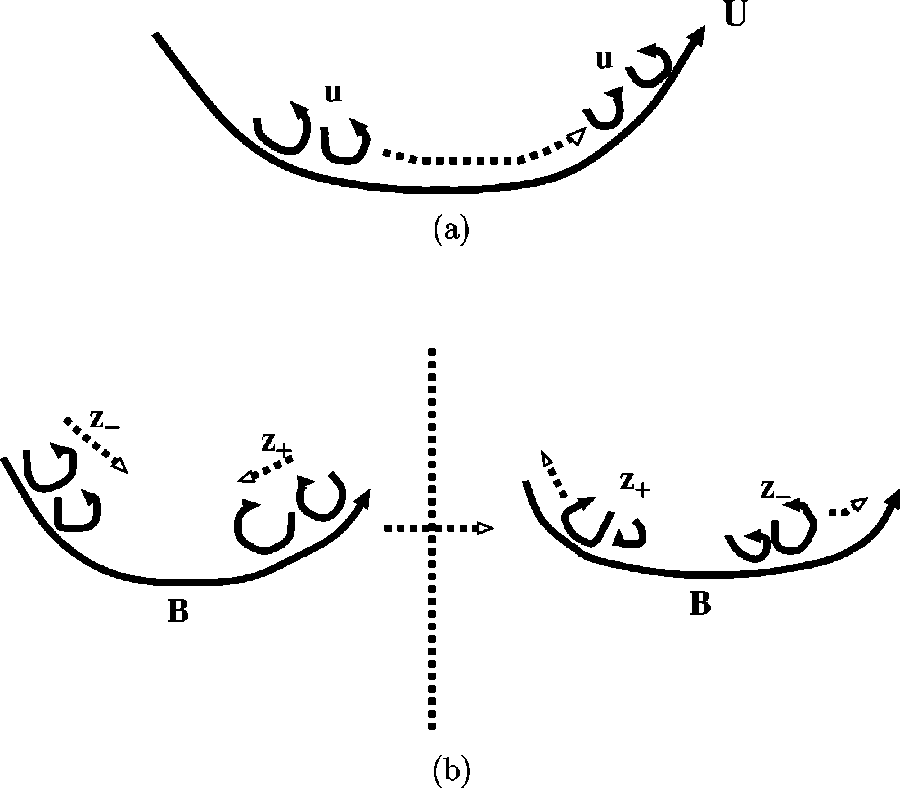
\includegraphics[width=0.7\columnwidth]{Fundamentos/fig1.png}
  \caption{Comparación entre hidrodinámica y magnetohidrodinámica: (a)
    En hidrodinámica, un flujo medio de gran escala barre
    (\emph{sweeps}) \emph{eddies} de escalas más pequeñas, sin
    afectar la transferencia de energía entre escalas
    longitudinales. (b) En magnetohidrodinámica, un campo magnético
    $\vec{B}$ de gran escala barre fluctuaciones $\vec{z}^-$ y
    $\vec{z}^+$ que se propagan en sentidos opuestos, lo cual afecta
    la transferencia de energía (ilustrado como distorsiones luego de
    que los dos tipos de fluctuaciones se hayan atravesado).}
  \label{fig:HDvsMHD}
\end{figure}



Por su parte, el flujo de gran escala arrastra los vórtices de menor
escala, pero sin inducir una distorsión apreciable en sus estructuras
dinámicas internas. La interacción directa entre las grande escalas y
las pequeñas consiste, entonces, en el movimiento de \textit{sweeping}
(o \textit{barrido}), que no involucra transferencia energética
significativa en el espacio de Fourier, ni cambia la forma del
espectro energético hidrodinámico. Esto se encuentra diagramado en la
figura \ref{fig:HDvsMHD}(a).

En cambio, las correlaciones temporales, o equivalentemente la forma
del espectro de frecuencias (obtenida a partir de la serie temporal de
la velocidad en un punto fijo), puede encontrarse fuertemente
influenciada por el efecto del \textit{sweeping}, dado que cualquier
fluctuación en una pequeña escala (que viene dada por movimientos de
\textit{straining}), será advectada y pasará a través del punto de
prueba, introduciendo así fuertes fluctuaciones en la serie temporal.

La aproximación de Taylor de turbulencia \textit{congelada}
(\textit{frozen turbulence}, \cite{taylor_spectrum_1938}) asume que el
flujo de gran escala, con velocidad $\vec{U}$, barre la turbulencia
del punto de observación. Esta aproximación, con una velocidad
constante y grande $U$ ($\gg u$, la velocidad de las fluctuaciones),
es utilizada en los estudios en túneles de viento y en los estudios de
la turbulencia en viento solar de una única nave espacial
\cite{jokipii_turbulence_1973}, con el objeto de poder convertir las
correlaciones temporales en espaciales. En líneas generales, la idea
es que el flujo de gran escala $U$ barre las fluctuaciones locales a
través del punto de observación más rápidamente de lo que las no
linealidades locales pueden producir distorsiones. Entonces, el
espectro de frecuencias tiene la misma forma que el de números de
onda, $E(\omega) \sim \epsilon^{2/3} U^{2/3} \omega ^{-5/3}$. El
\textit{sweeping} por flujos aleatorios (con un valor grande pero
aleatorio de $\vec{U}$) da un resultado similar
\cite{tennekes_eulerian_1975, chen_sweeping_1989}. En constraste,
cuando el barrido es despreciable comparado con los movimientos de
\textit{straining}, el espectro puede ser predicho por análisis
dimensional, requiriendo que la densidad espectral en frecuencias
dependa exclusivamente de la velocidad de la cascada de energía y de
la frecuencia \cite{tennekes_eulerian_1975, nelkin_time_1990}. Esto
implica que $E(\omega) \sim \epsilon \omega^{-2}$. De esta forma, la
presencia o ausencia de un flujo $U$ en las grandes escalas resulta
relevante para el espectro de frecuencias, si se asume la hipótesis de
\textit{sweeping}.

Por otra parte, resulta bastante claro que el \textit{sweeping} no
entra directamente en consideración en la forma que adopta el espectro
energético hidrodinámico en la \cref{eq:Ek}
\cite{chapman_computational_1979}. Sin embargo, hay una relación
claramente establecida entre el \textit{sweeping} y los momentos de
orden más alto (por ejemplo, función de esctructura y espectro de
energía cinética) \cite{nelkin_time_1990}. En particular, la
influencia que el \textit{sweeping} aleatorio ejerce en el espectro de
frecuencias puede traducirse directamente en una influencia similar en
el espectro de densidad de energía cinética (momento de cuarto orden)
\cite{chen_sweeping_1989}. Este resultado se condice con resultados
experimentales \cite{van_atta_higher-order_1975,
  zhou_non-gaussian_1993}, que muestran que los espectros de momentos
de orden más alto en el rango inercial tienen los mismos exponentes en
la ley de potencias que el espectro energético, en lugar de los
valores que tendrían suponiendo sólo argumentos de \textit{straining}
puro. Estos experimentos demuestran la importancia del efecto de
barrido, la multiplicidad de escalas temporales y el rol de la no
localidad.

\subsection{Escalas temporales, cascada y clausura}

¿Cómo pueden agregarse los efectos de las escalas temporales
adicionales en una teoría simple de espectros turbulentos? Una
posibilidad es mirar con más detenimiento los conceptos físicos de la
\cref{eq:transferRate}. Supongamos que escribimos la tasa de
transferencia o el flujo de energía en la forma (mucho más sugestiva)
\begin{equation}\label{eq:TR_sw}
  \epsilon = \Pi(k) = \frac{u_k^2}{\tau_{sp}}.
\end{equation}
Aquí, $u_k^2$ es el doble de la energía por unidad de masa asociada a
la velocidad a escalas cercanas a $1/k$. Por compatibilidad con las
\cref{eq:transferRate,eq:tauNL}, podemos identificar el tiempo de
transferencia de energía como $\tau_{sp} = \tau_{nl}^2/\tau_T(k)$. En
consecuencia, desarrollando diferentes aproximaciones para el tiempo
$\tau_T$ de la triple correlación, es posible obtener una variedad de
modelos para los espectros de turbulencia.

El significado más profundo de este procedimiento simbólico puede ser
visto examinando cómo relaciones similares a las dadas por las
\cref{eq:transferRate,eq:TR_sw} emergen en un tratamiento
matemáticamente más formal, y cuánto más precisas se vuelven las
definiciones de las escalas temporales que entran en las teorías al
asociarlas con términos que aparecen fenomenológicamente.

Una forma particularmente reveladora de la ecuación de evolución para
el espectro energético emerge de la clausura conocida como
aproximación Markoviana cuasinormal de remolinos amortiguados
(\textit{eddy-damped, quasinormal Markovian}, o \textit{EDQNM} por sus
siglas). Como una breve introducción \cite{orszag_analytical_1970,
  monin_statistical_2013, mccomb_physics_1990,
  lesieur_turbulence_2008}, analicemos la parte más estructural de
este enfoque.  Consideremos la ecuación de Navier-Stokes en el espacio
de momentos, $\partial_t \hat{u}(\vec{k}) = \hat{u}\hat{u} - \nu k^2
\hat{u}(\vec{k})$ \cite{lesieur_turbulence_2008}, donde $\hat{u}$
refiere a la representación de Fourier del campo de velocidades y se
presuponon los índices cartesianos y la sumatoria sobre índices. La
ecuación para el espectro modal $E(k)/4\pi k^2 \sim \langle
\hat{u}\hat{u} \rangle$ tiene la forma
\begin{equation}\label{eq:2ndorder}
  \left(\frac{\partial}{\partial t} + \nu k^2 \right) \langle \hat{u} \hat{u} \rangle = \langle \hat{u} \hat{u} \hat{u} \rangle.
\end{equation}
Esto involucra momentos de tercer orden (correlaciones triples)
$\hat{u}\hat{u}\hat{u}$, que obedecen una ecuación de la forma
\begin{equation}\label{eq:3rdorder}
  \left(\frac{\partial}{\partial t} + \nu \left(k^2+p^2+q^2\right) \right) \langle \hat{u}(\vec{k}) \hat{u}(\vec{p}) \hat{u}(\vec{q}) \rangle = \langle \hat{u} \hat{u} \hat{u} \hat{u} \rangle,
\end{equation}
donde $\vec{k}$, $\vec{p}$ y $\vec{q}$ denotan vectores de onda. El
``problema de clausura'' se refiere a la ocurrencia de correlaciones
de cuarto orden en las ecuaciones para la correlación de tercer orden,
correlaciones de quinto orden en las ecuaciones para cuarto orden, y
así sucesivamente, no siendo posible clausurar el problema a ningún
orden. Los métodos de clausura adoptan aproximaciones para momentos de
orden más alto en términos de momentos de órdenes más bajos. La
aproximación cuasinormal (QNA, \cite{millionshchikov_1941}) representa
el momento de cuarto orden de la \cref{eq:3rdorder} como una suma
sobre productos de momentos de segundo orden. Esto permite encontrar
una solución para los momentos de tercer orden, que se pueden
sustituir entonces en la \cref{eq:2ndorder}, dando lugar a un sistema
de ecuaciones cerrado para los momentos de segundo orden, y en
consecuencia para el espectro de energía. Orszag
\cite{orszag_analytical_1970} y otros introdujeron refinamientos
adicionales y aproximaciones que dan lugar a la aproximación
\textit{EDQNM}. Este es en muchos aspectos un modelo aceptable para
turbulencia, y conduce a una ecuación para el espectro, que puede ser
escrita como
\begin{equation}\label{eq:spectrumeq}
  \left( \frac{\partial}{\partial t} + \nu k^2 \right) E(k, t) = \int\int_\Delta dp dq \Theta_{kpq} E(q,t) \times \left[ A(k, p, q) E(q, t) - B(k, p, q) E(k, t)\right].
\end{equation}

Aquí, las integrales son sobre todos los vectores de onda con la
restricción $\vec{q} = \vec{k} - \vec{p}$, y $A$ y $B$ son
coeficientes de acoplamiento con unidades de número de onda.  El
tiempo $\Theta_{kpq}$ aparece como un tiempo característico de
relajación debido a las transferencias no lineales y a la viscosidad
de $\langle \hat{u}(\vec{k}) \hat{u}(\vec{p}) \hat{u}(\vec{q})
\rangle$.  El flujo de energía en el rango inercial puede ser
calculado a partir de la integral $\Pi(k) = -\frac{\partial}{\partial
  t} \int_0^k E(k, t) dk$, utilizando la expresión \textit{EDQNM} en
el miembro derecho de la \cref{eq:spectrumeq}. Finalmente, estimando
que las contribuciones dominantes provienen de $p \approx q \approx
k$, se llega a $\epsilon = \Pi(k) = \tau_T(k) k^4 E^2(k)$, previamente
obtenido por análisis dimensional en el rango inercial. Cabe notar que
el ``tiempo de decaimiento triple'' $\tau_T(k)$, que anteriormente
asumimos que aparecía por argumentos heurísticos, es ahora
identificable con \textit{eddy-damping time} $\Theta_{kkk}$ (o
``tiempo de amortiguación de los remolinos'') que emerge como el
tiempo clave en la evaluación del flujo de energía
\textit{EDQNM}. Este resultado nos da confianza, porque ahora el
resultado dimensional adquiere un contexto dentro de la teoría
analítica. Sin embargo, es muy importante tener en cuenta que el rol
físico que cumple la tasa de amortiguamiento de los \textit{eddies} en
la correlación triple es el de restaurar, de una forma aproximada, el
efecto de descorrelación de los cumulantes de tercer orden, que
habíamos despreciado en la QNA. En efecto, la elección del
\textit{eddy-damping rate} conlleva que la aproximación \textit{EDQNM}
tenga una ley espectral particular. De esta forma, a pesar de la
elegancia algebraica, la clausura \textit{EDQNM} requiere que
entendamos correctamente la física que determina el tiempo de
descorrelación. Aún así, la identificación $\tau_T(k) = \Theta_{kkk}$
nos da confianza respecto de cómo tales escalas de tiempo actúan en
teorías más formales, mientras que nos da una cadena de razonamiento
que conecta el análisis dimensional con la estructura matemática de la
turbulencia. Este es un marco útil cuando extendemos el uso de las
cascadas fenomenológicas para incluir otras escalas de tiempo (y sus
efectos) en MHD.

Otra teoría de clausura, la Aproximación de Interacción Directa de
Kraichnan (\textit{DIA}, por sus siglas en inglés, 1957), quizás el
arquetipo de teorías de clausura estadísticas de turbulencia, procede
a través de una expansión de perturbaciones en las que el orden más
bajo de la velocidad obedece exactamente la estadística gaussiana. La
\textit{DIA} busca una solución al problema de clausura en turbulencia
expandiendo en un parámetro $\delta$, permitiendo que los términos no
lineales en la ecuación de evolución sean del orden de $\delta$, que
eventualmente se igualará a la unidad. Para facilitar la solución, se
define un propagador (una función de Green) $\tilde{G}(\vec{k}, t,
t')$, el cual representa la respuesta del sistema a una función
gaussiana de forzado del sistema correlacionada con $\delta$. Un punto
clave es obtener las ecuaciones acopladas de renormalización para el
propagador promediado $G = \langle\tilde{G}\rangle$ y para la función
espectral retrasada $Q(\vec{k}, t, t')$, que determina cuán
rápidamente las correlaciones decaen en el tiempo. Cabe mencionar que
la correlación de dos puntos espacio-temporales puede definirse como
$R_{ij}(\vec{r}, \tau) = \langle u_i(\vec{x}, t) u_j(\vec{x}+\vec{r},
t+\tau)\rangle$, mientras que el tensor espectral retrasado en el
tiempo $S_{ij}(\vec{k},\tau)$ la la transformada de Fourier espacial,
con la componente temporal (el retraso temporal) ahora denotando la
descorrelación temporal de ambos elementos del espectro. La función
espectral $Q$ de DIA es, esencialmente, la traza de $S$.

Mientras los detalles no son importantes para el presente trabajo (ver
\cite{leslie_developments_1973, mccomb_physics_1990}), la solución
simultánea para $Q$ y $G$ establece la naturaleza de dos tiempos de
descorrelación en cada número de onda. Acordemente, en el formalismo
del propagador, la dependencia temporal de las correlaciones de tercer
orden se encuentra establecida en términos de las correlaciones de
segundo orden.

En general, los modelos de \textit{EDQNM} y \textit{DIA} son bastante
distintos, pero McComb \cite{mccomb_physics_1990} argumenta que hay
una interestante modificación \textit{ad hoc} a \textit{DIA} que
muestra una conexión estructural entre ambos modelos. Supongamos que
en lugar de resolver las ecuaciones isotrópicas de \textit{DIA} para
$Q$ y $G$ de la forma usual, empezamos con \textit{DIA} y hacemos la
simple aproximación, para $t>t'$, $Q(\vec{k}, t, t') = S(\vec{k}, t')
e^{-\gamma(k) (t-t')}$ y $G(\vec{k}, t, t') = e^{-\gamma(k)(t-t')}$,
donde la tasa de descorrelación es tomada para ser el recíproco del
tiempo no lineal, $\gamma(k) = 1/\tau_{nl}(k) \sim \epsilon^{1/3}
k^{2/3}$. En este caso, esta ecuación ``pseudo - \textit{DIA}'' para
la evolución espectral se vuelve idéntica a la ecuación espectral de
\textit{EDQNM}, la \cref{eq:spectrumeq}. Esta identificación no debe
ser tomada muy seriamente, ya que \textit{DIA} prescribe el tiempo de
descorrelación a su manera. Sin embargo, en la medida en que el límite
de McComb es realizable, la aproximación \textit{EDQNM}, el
\textit{DIA} modificado y el enfoque fenomenológico concuerdan: la ley
espectral de potencias viene determinada por la elección de la escala
temporal $\Theta_{kpq}$. Entonces, resulta razonable buscar un
tratamiento fenomenológico del espectro MHD para entender la variedad
de conclusiones que pueden ser aplicables al espacio y a plasmas
astrofísicos.




\section{Turbulencia magnetohidrodinámica}\label{sec:turbulenciaMHD}

\subsection{Ecuaciones MHD y conceptos físicos básicos}

Habiendo hecho un análisis básico de cómo las diferentes escalas
temporales aparecen en el caso de turbulencia hidrodinámica, veamos
ahora el caso magnetohidrodinámico, en el cual, si bien es más
complejo, es posible aplicar algunas de las ideas para entender qué
espectro son esperables.

Un plasma, descripto como un fluido eléctricamente conductor,
evoluciona en respuesta a fuerzas tanto mecánicas como
electromagnéticas. Por simplicidad, nos focalizaremos en el modelo
incompresible con densidad constante, que provee un contexto adecuado
para muchos de los problemas de turbulencia MHD
\cite{biskamp_magnetohydrodynamic_2003}. El modelo MHD incompresible,
en términos de la velocidad $\vec{u}$ del fluido y del campo magnético
$\vec{B}$, consta de una ecuación de momentos
\begin{equation}\label{eq:NS-MHDu}
  \frac{\partial \vec{u}}{\partial t} + \vec{u} \cdot \nabla\vec{u} = -\frac{1}{\rho} \nabla p + \frac{1}{4\pi\rho} \left(\nabla\times\vec{B}\right)\times\vec{B} + \nu \nabla^2 u,
\end{equation}
y de una ecuación de inducción magnética
\begin{equation}\label{eq:NS-MHDB}
  \frac{\partial \vec{B}}{\partial t} = \nabla \times \left(\vec{u}\times\vec{B}\right) + \mu \nabla^2 \vec{B}.
\end{equation}
La densidad del plasma $\rho$, la viscosidad cinemática $\nu$ y la
difusividad magnética $\mu$ se consideran uniformemente constantes. La
velocidad y el campo magnético son solenoidales,
$\nabla\cdot\vec{u} = \nabla\cdot\vec{B} = 0$, y la presión $p$ está
determinada por la divergencia de la \cref{eq:NS-MHDu}. El número de
Reynolds $R = uL/\nu$ (donde $u$ es una velocidad típica y $L$ es una
escala espacial típica) y el número de Reynolds magnético
$R_m = uL/\mu$ miden el peso relativo entre los términos no lineales y
los términos lineales disipativos en las ecuaciones dinámicas. Se
tiene MHD altamente turbulento cuando los valores de $R$ y $R_m$
suficientemente altos.

Antes de continuar, recordemos que el modelo MHD es frecuentemente
aplicado al espacio y a plasmas astrofísicos. No obstante, en ninguno
de estos casos suele ser clara la derivación del modelo. Para plasmas
poco colisionales, la estructura básica de MHD emerge por las
conservaciones de la masa, el momento y la energía, junto con las
leyes de Maxwell-Ampère y Faraday, e ignorando las corrientes de
desplazamiento y adoptando una forma adecuada de la ley de Ohm. Aún
así, para la mayoría de las aplicaciones no hay un camino claro para
cerrar el sistema con un único campo de presiones isótropo, ni hay
cálculos convicentes para la viscosidad, la resistividad, y otros
coeficientes de transporte como la conductividad térmica.

Un camino posible para trabajos numéricos es adoptar coeficientes
disipativos escalares, eligiendo los valores de acuerdo a las
limitaciones numéricas de resolución espacial, más que en el realismo
físico. Para MHD turbulento esto puede estar justificado asumiendo que
la cascada no lineal se da principalmente desde las escalas grandes a
las pequeñas, y el papel específico de la disipación mecánica es el de
absorber cualquier energía que llegue a escalas pequeñas vía
transferencia espectral. Esto es parcialmente satisfactorio, y sería
deseable un mayor comprendimiento teórico de la naturaleza de la
disipación en las aplicaciones de MHD poco colisional, aunque puede no
ser simple ni tener una forma universal. Por el lado positivo, cuando
se tienen observaciones experimentales disponibles, como es en el caso
del viento solar, se puede ver que el rango inercial es amplio, por lo
que el rango \textit{energy-containing} se encuentra bien separados en
escala del rango disipativo, donde el espectro se vuelve más empinado
\cite{leamon_observational_1998}. Con esta base, es posible inferir un
Reynolds efectivo para el viento solar, y por analogía para cualquier
plasma turbulento cuyo rango inercial sea conocido. Por ejemplo,
ignorando las diferencias entre la disipación viscosa y resistiva, uno
podría emplear una estimación hidrodinámica para el número de onda
disipativo, $k_d = \left(\epsilon/\nu^3\right)^{1/4}$. Usando la
estimación de Taylor-von Karman de la tasa de decaimiento $\epsilon =
u^3/\lambda$, puede escribirse $k_d \lambda = R^{3/4}$, o $R =
\left(k_d \lambda\right)^{4/3}$, donde $R$ es el número de
Reynolds. La cantidad $k_d \lambda$ es aproximadamente el ancho de
banda del rango inercial. De esta forma, para un rango inercial de
tres a cuatro décadas (por ejemplo, el viento solar), uno tiene $R
\approx 10^5$. Para la corona solar, se estima un rango inercial de
cinco a seis décadas, por lo que $R \approx 10^8$. En general, cuando
hay un rango inercial de varias décadas, uno puede inferir que el
Reynolds efectivo para las grandes escalas es un número grande, aún
cuando no se tenga una formulación teórica del mecanismo de
disipación.

El campo magnético puede contener una parte uniforme $\vec{B}_0$
(campo magnético DC) o que varía muy suavemente (identificable con el
campo magnético medio local), más fluctuaciones de pequeña escala
$\vec{b}$, es decir, $\vec{B} = \vec{B}_0 + \vec{b}$. El campo
magnético de gran escala permite y respalda la propagación de ondas
hidromagnéticas (ondas de Alfv\'en). Estas ondas son fluctuaciones
transversales al campo magnético medio, propagándose en la dirección
de campo magnético medio a la velocidad de Alfv\'en
$V_A = B_0/\sqrt{4\pi\rho}$.

Aún el caso más simple de MHD, asumiendo incompresibilidad, isotropía,
estacionariedad y homogeneidad, es más complejo que el caso
hidrodinámico. Hay dos campos distintos con los que hay que lidiar, el
magnético y el de velocidades, y se agrega complejidad debido al
efecto de la propagación de ondas de Alfv\'en. De esta forma, hay al
menos dos clases de escalas temporales involucradas, el tiempo no
lineal y el tiempo de Alfv\'en (el tiempo para que una fluctuación se
propague dada una escala espacial). Es más, el campo magnético de gran
escala introduce una dirección preferencial, y los efectos
anisotrópicos que esto genera se hacen presentes en las fluctuaciones.

Aquí hemos arribado a una gran diferencia entre turbulencias
hidrodinámica y magnetohidrodinámica. A diferencia del caso
hidrodinámico, el efecto no local de las escalas grandes sobre las
pequeñas, el \textit{sweeping}, tiene un papel importante en
turbulencia MHD. De hecho, comenzando por Iroshnikov (1964,
\cite{iroshnikov_turbulence_1964}) y Kraichnan (1965,
\cite{kraichnan_inertial-range_1965}), hay argumentos para plantear
que el \textit{sweeping} juega un papel importante aún en el caso de
ausencia de campo magnético DC. Si hay un campo magnético fuerte de
gran escala, las fluctuaciones de pequeña escala sufren un efecto
similar al \textit{sweeping} debido a la propagación de ondas de
Alfv\'en. Para discutir esto, es más fácil escribir las ecuaciones MHD
en una forma más simétrica, utilizando los denominados campos de
Els\"asser \cite{elsasser_hydromagnetism_1956}, $\vec{z}^\pm = \vec{u}
\pm \vec{b}/\sqrt{4\pi\rho}$,
\begin{equation}\label{eq:MHDElsasser}
  \frac{\partial \vec{z}^\pm}{\partial t} \mp \vec{V_A} \cdot \nabla\vec{z}^\pm = -\vec{z}^\mp \cdot \nabla\vec{z}^\pm - \frac{1}{\rho} \nabla P + \mu \nabla^2 \vec{z}^\pm,
\end{equation}
donde hemos explícitamente separado el término que involucra el campo
magnético de gran escala (escrito en términos de la velocidad de
Alfv\'en $\vec{V_A}$). Por simplicidad, hemos asumido $\nu = \mu$. La
presión total $P = p + B^2/8\pi$ actúa de manera de hacer cumplir la
condición $\nabla\cdot\vec{z}^\pm = 0$.

Eligiendo o bien $\vec{z}^+ = 0$ o bien $\vec{z}^- = 0$, obtenemos las
soluciones exactas de las ecuaciones MHD ideales (sin disipación). El
campo no nulo normalmente se dice que corresponde a paquetes de onda
que se propagan a lo largo de la dirección de campo medio. Esta
descripción puede ser confusa, pues los ``paquetes'' pueden no estar
localizados ni propagándose. Las fluctuaciones no propagantes con
vectores de onda perpendiculares a la dirección del campo magnético
medio tienen velocidad de fase nula. En cualquier caso, ambos tipos de
fluctuaciones $\vec{z}^\pm$ son necesarias para que los términos no
lineales sean no nulos y haya turbulencia. Este hecho fue apuntado por
Kraichnan \cite{kraichnan_inertial-range_1965}, y discutido en el
contexto de aplicaciones en física espacial
\cite{dobrowolny_fully_1980} y en los modelos de calentamiento de la
corona solar \cite{dmitruk_conditions_2001}.

Kraichnan \cite{kraichnan_inertial-range_1965} señaló que el campo
magnético medio barre las estructuras a pequeña escala con las que
interactúa, y durante ese momento se produce una transferencia no
lineal de energía entre distintas escalas longitudinales (en la
representación de Kraichnan, los paquetes de onda sufren breves
``colisiones'' durante las cuales ocurre transferencia de
energía). Esto se ilustra en la figura \ref{fig:HDvsMHD}(b). De esta
manera, las escalas pequeñas interactúan no sólo a través de los
\textit{eddies}, sino también a través de los paquetes Alfv\'en, que
reducen el flujo de energía a escalas pequeñas al aumentar su tiempo
de transferencia \cite{chen_inhibition_1997}. Esto introduce en la
práctica una interacción no local a medida que las ondas se propagan a
lo largo del campo a gran escala \cite{gomez_validity_1999}.



Para flujos turbulentos MHD con un número de Reynolds alto, en
entornos astrofísicos y espaciales, existe una separación de escala
entre distintos procesos físicos a grandes y pequeñas
escalas. Específicamente, se divide la dinámica en una parte de
pequeña escala, que contiene acoplamientos de escalas
``pequeña-pequeña'' y ``pequeña-grande'', y en otra parte, de gran
escala \cite{zhou_transport_1990}. Cuando los campos de pequeña escala
ocupan un amplio ancho del espectro, se tiende a tratar el
acoplamiento de escalas ``pequeña-pequeña'' como turbulento,
involucrando acoplamientos que son principalmente locales en el
espacio de escalas.

El estudio de turbulencia MHD en los contextos espaciales y
astrofísicos a menudo se vuelven manejables cuando se introduce alguna
forma de separación de escala. En la aproximación más simple, una
pequeña parte de un sistema MHD no homogéneo podría tratarse como
``localmente homogéneo''. La turbulencia en el viento solar es un
ejemplo posible, en el que adicionalmente hay muchas mediciones que
hacen posible la corroboración teórica a partir de observaciones
\cite{tu_mhd_1995, goldstein_magnetohydrodynamic_1995}. Los primeros
estudios observacionales \cite{coleman_turbulence_1968} encontraron
que las fluctuaciones temporales de la velocidad del plasma, desde el
punto de referencia de una nave espacial, admiten una ley de potencias
para el espectro de escalas, un reminiscente de la descripción de
Kolmogorov de la turbulencia de un fluido. Las observaciones también
revelaron una correlación distintiva entre la velocidad y el campo
magnético, que sugiere la presencia de ondas de Alfv\'en
\textit{outward-traveling} de gran amplitud
\cite{coleman_turbulence_1968, belcher_large-amplitude_1971,
jokipii_turbulence_1973}.

El viento solar, como la mayoría de los sistemas astrofísicos reales
en los que se encuentra turbulencia, es compresible e inhomogéneo a
grandes escalas. Las inhomogeneidades de gran escala, como cizallas de
velocidad o gradientes de temperatura y densidad, pueden suministrar
energía a la turbulencia de pequeña escala. En el viento solar, las
fluctuaciones observadas se dan en todas las escalas, con escalas de
correlación ($\lambda \sim 0.02$AU en la órbita terrestre) mucho más
pequeñas que la escala del sistema ($1$AU o más). El rango inercial de
la turbulencia MHD se extiende desde $\lambda$ hasta escalas 1000
veces más chicas, cercanas a la giroescala térmica de los
iones. Entonces, la actividad turbulenta de interés está bien
separada, en escalas de longitud, de las inhomogeneidades de gran
escala del viento solar. Es más, las propiedades de gran escala, tales
como el flujo medio y el campo magnético medio, son relativamente
coherentes y reproducibles. Entonces, el viento solar suele ser
descripto en términos del flujo canónico promedio y de propiedades del
campo magnético, tales como viento tranquilo de baja velocidad a bajas
latitudes; viento caliente, menos denso y más rápido a altas
latitudes; una espiral de Arquímedes, y otras idealizaciones con
carácterísticas de gran escala. Aún cuando están presentes estructuras
dinámicas de gran escala, estas características pueden verse con
cierto grado de reproducibilidad.

En contraste, las fluctuaciones del campo observables en las pequeñas
escalas del viento solar, suelen verse como aleatorias y localmente
homogéneas. Estas fluctuaciones fueron tratadas originalmente
utilizando MHD linealizado débilmente inhomogéneo (teoría WKB)
\cite{parker_dynamical_1965, hollweg_alfven_1973,
  hollweg_transverse_1974, hollweg_transition_1986,
  jacques_momentum_1977, matthaeus_transport_1994}, que describe la
propagación de fluctuaciones Alfv\'enicas de onda corta en un flujo
inhomogéneo. La presente perspectiva es que el medio es localmente
incompresible \cite{matthaeus_evidence_1990} y es descripto
aceptablemente como turbulencia MHD.

La dicotomía entre la representación de ``turbulencia'' no lineal y la
representación de ``ondas'' lineales se empapa de 40 años de estudio
del viento solar y espeja el tema básico del presente trabajo: las
características observables de la turbulencia MHD emergen de un
balance entre la propagación de ondas y el \textit{sweeping}, por un
lado, y las distorsiones o \textit{strainings}, por otro.


\subsection{Fenomenología del decaimiento MHD}
Mientras en turbulencia hidrodinámica lidiamos con una única densidad
de energía $u^2$ y un único tensor de correlación de dos puntos
asociado, la presencia de dos campos dinámicos en MHD introduce cuatro
tipos de correlaciones o energías (por unidad de masa): la energía
cinética $E_u = \langle \left| \vec{u}\right|^2\rangle/2$, la energía
magnética $E_b = \langle \left| \vec{b}\right|^2\rangle/2$, la
helicidad cruzada $H_c = \langle \vec{u} \cdot \vec{b} \rangle =
\langle \left| \vec{z}^+\right|^2 - \left| \vec{z}^-\right|^2
\rangle/4$ y la diferencia de energías $D = \langle \left|
\vec{u}\right|^2 - \left| \vec{b} \right|^2 \rangle/2 = \langle
\vec{z}^+ \cdot \vec{z}^- \rangle/2$. (Se utilizan unidades de
velocidad de Alfvén, en la que el campo magnético $\vec{b} \rightarrow
\vec{b}/\sqrt{4\pi\rho}$ tiene dimensiones de velocidad.) Notar que la
helicidad cruzada es la diferencia de las energías de Els\"asser
$Z_\pm^2 = \langle \left| \vec{z}^\pm \right|^2 \rangle/4$. La
situación más simétrica se da cuando se tiene equipartición, $D = 0$ y
$H_c = 0$. Para este caso, ni los campos magnético y de velocidades,
ni las variables de Els\"asser, se encuentran correlacionadas entre
sí. En este tipo de MHD, $Z_-^2 = Z_+^2 = Z^2$, y una simple extensión
de la fenomenología del decaimiento hidrodinámico funciona bien para
MHD con un número de Reynolds moderado
\cite{hossain_phenomenology_1995}. En particular, $dZ^2/dt = -\alpha
Z^3/\lambda$ y $d\lambda/dt = \beta Z$, donde $\alpha$ y $\beta$ son
constantes de orden uno y $\lambda$, una similaridad o
\textit{energy-containing scale}. La elección de las constantes puede
tener una interpretación física como en el caso hidrodinámico
\cite{matthaeus_anisotropic_1996}. Este enfoque de tipo hidrodinámico
para el decaimiento MHD se ha utilizado en el modelado del transporte
de la turbulencia en el viento solar; dicho modelo proporciona una
explicación razonablemente precisa del perfil radial de la turbulencia
del viento solar, desde la órbita terrestre ($1$AU) hasta más de
$60$AU \cite{smith_heating_2001}.

Más generalmente, no se puede asumir helicidad cruzada nula, y la
fenomenología del decaimiento debe tener en consideración la asimetría
entre $Z_+^2$ y $Z_-^2$. Esto introduce escalas de tiempo
adicionales. Las bases de esto se encuentran, por ejemplo, en las
discusiones fenomenológicas de Iroshnikov
\cite{iroshnikov_turbulence_1964}, Kraichnan
\cite{kraichnan_inertial-range_1965} y Dobrowolny
\cite{dobrowolny_fully_1980}, y en el tratamiento detallado de
clausuras MHD por Pouquet \cite{pouquet_strong_1976} y Grappin
\cite{grappin_dependence_1983}. La aproximación fenomenológica
propuesta por Hossain \cite{hossain_phenomenology_1995} plantea que
\begin{equation}
  \frac{dZ_\pm^2}{dt} = -\alpha_\pm \frac{Z_\pm^2}{\tau_{sp}^\pm}
\end{equation}
en términos de las constantes $\alpha_+$ y $\alpha_-$, de forma
similar a lo ya expuesto para hidrodinámica. La estimación más simple
\cite{pouquet_strong_1976, grappin_dependence_1983} es que el tiempo
de transferencia espectral se identifique con el tiempo de
\textit{eddy turnover} (tiempo no lineal), es decir, $\tau_{sp}^\pm =
\tau_{nl}^\pm$; mientras que este último, teniendo en cuenta la
naturaleza de las interacciones entre $\vec{z}^+$ y $\vec{z}^-$, puede
ser estimado como $\tau_{nl}^\pm = \lambda_\pm / Z_\mp$ para escalas
de similaridad $\lambda_\pm$. Para esta elección, la ecuación de
decaimiento de la energía se puede escribir como
\begin{equation}\label{eq:elsasserdecay}
  \frac{dZ_\pm^2}{dt} = -\alpha_\pm \frac{Z_\pm^2 Z_\mp}{\lambda_\pm}
\end{equation}

Para cerrar el sistema de ecuaciones del decaimiento, se debería
elegir (y verificar si es posible) una ecuación de evolución para las
escalas de similaridad $\lambda_\pm$. Una posibilidad es
$d\lambda_\pm/dt = \beta_\pm (Z_+Z_-)^{1/2}$
\cite{hossain_phenomenology_1995}, pero se mantiene cierta dificultad
en verificar el comportamiento de las escalas de similaridad, puesto
que deben resolverse (en, por ejemplo, las simulaciones), tanto las
escalas más pequeñas (de manera de resolver adecuadamente la cascada
directa de energía) como las escalas más grandes.

Otra dificultad con el decaimiento MHD fenomenológico es el grado de
certeza y generalidad con el que se hace la identificación
$\tau_{sp}^\pm \rightarrow \tau_{nl}^\pm$, utilizada en la
\cref{eq:elsasserdecay}. Efectivamente, cabe preguntarse si hay alguna
otra escala temporal que entre en juego en el decaimiento global, por
ejemplo, algún otro tipo de escala tipo \textit{sweeping} que pueda
descorrelacionar las interacciones de las grandes escalas no lineales,
modificando así la tasa global de decaimiento de energía. Dichas
cuestiones serán discutidas a continuación, en el contexto del rango
inercial de la turbulencia MHD, para los casos tanto isotrópico como
anisotrópico de MHD, éste último con la presencia de un campo
magnético de gran escala.

Sin embargo, para el rango de escalas de \textit{energy-containing},
ese problema continúa ambiguo. Para turbulencia homogénea periódica,
Hossain y otros \cite{Hossain_solar_1996} plantearon que el desarrollo
de una anisotropía relativa a un campo magnético de gran escala actúa
saturando y minimizando el efecto de descorrelación en el rango de
escalas energéticas. Sin embargo, esto presupone que el tiempo de
Alfv\'en de gran escala $\tau_A = \lambda/V_A$ es no demasiado
pequeño. Esto puede depender de las condiciones iniciales, tanto como
de las condiciones de contorno. Un tema particularmente sensible en
las aplicaciones \cite{dmitruk_conditions_2001} es si las condiciones
de contorno permiten la persistencia de estructuras no propagantes,
tales como turbulencia 2D, que no son afectadas por el tiempo de
barrido debido a ondas de Alfv\'en, $\tau_A$. Además, las
interacciones entre condiciones de contorno, efectos de propagación de
ondas, e interacciones no lineales, pueden tener un impacto en el
nivel de turbulencia (medido como tasa transferencial de energía)
mantenido por el sistema (\cite{dmitruk_lowfrequency_2003} para
aplicación en modelo de calentamiento coronal). Por ahora, sin
embargo, notamos que la multiplicidad de escalas temporales en MHD
puede afectar también la dinámica del rango de energías. En esos
casos, los detalles del problema específico pueden influir en el
tiempo de decaimiento energético. Para ciertos problemas estándar,
tales como MHD periódica u homogénea con condiciones
\textit{band-limited} iniciales (excitación de modos en ciertas
escalas limitadas), hay evidencia numérica que apoya la afirmación de
que el tiempo de decaimiento global está asociado mayoritariamente con
efectos no lineales, y que los efectos de los tiempos de sweeping y de
Alfv\'en no son significativos. Claramente, esta conclusión
necesitaría ponerse a prueba en otros problemas. Por ejemplo, el caso
de fluctuaciones de Els\"asser espacialmente localizadas, bajo la
influencia de un campo magnético DC \cite{parker_cosmical_2019} podría
presentar un contraste interesante al caso de turbulencia
homogénea. Con este trasfondo, veamos ahora el rol de escalas
temporales en las varias posibles cascadas MHD en el rango inercial.


\subsection{MHD isótropo}
\subsubsection{Cuando el \textit{straining} local es dominante: escaleo de
  Kolmogorov}

Montgomery y Fyfe \cite{fyfe_high-beta_1976} han sugerido que el
razonamiento original de Kolmogorov y el espectro $k^{-5/3}$ asociado
son aplicables a MHD. La suposición implicita es que el tiempo no
lineal de distorsión de \textit{eddies} es más rápido que el asociado
a propagación de ondas. Esto implica que la escala de tiempo relevante
es $\tau_{nl}$ y que el \textit{straining} domina sobre el
\textit{sweeping} aleatorio y la propagación de ondas. Este enfoque
parece razonable cuando la helicidad cruzada es pequeña, los campos
magnético y de velocidades se encuentran cercanos a equipartición, y
el campo magnético de grandes escalas no es demasiado grande.

\begin{figure}[h]
  \centering
  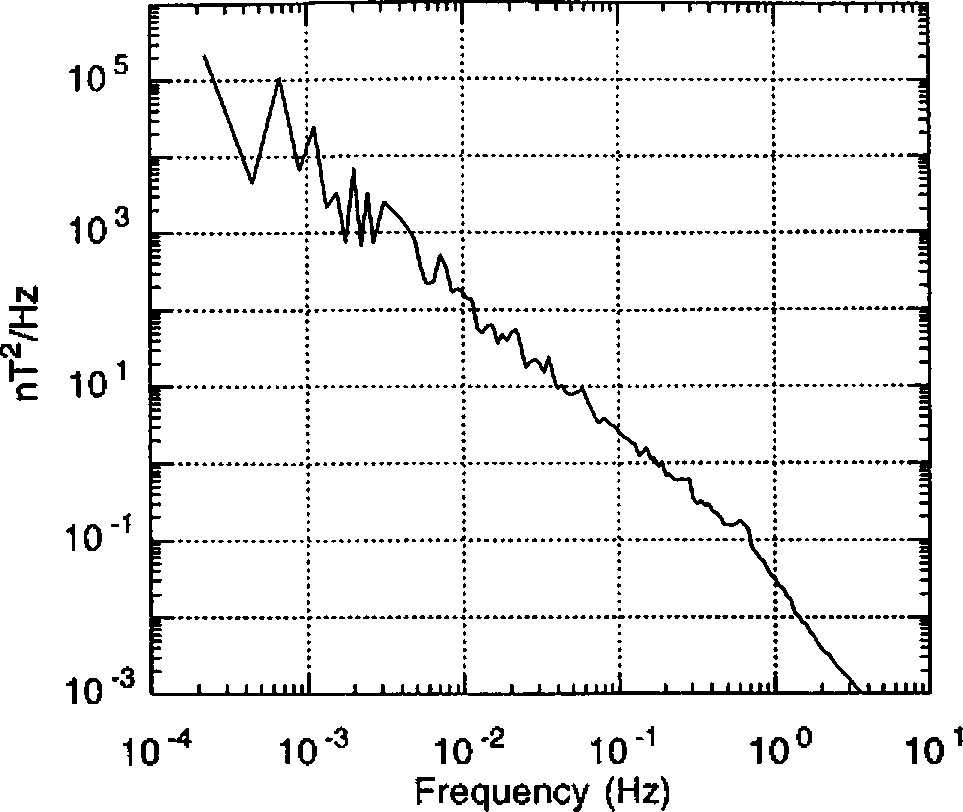
\includegraphics[width=0.7\columnwidth]{Fundamentos/fig2.png}
  \caption{Traza de la matriz espectral de potencias del campo
    magnético, medido por el magnetómetro Mariner 10 en 1974. Los
    resultados muestran que el espectro del viendo solar escala con la
    pendiente $-5/3$ de Kolmogorov. Adaptado de
    \cite{goldstein_magnetohydrodynamic_1995}.}
  \label{fig:experimentalcascade}
\end{figure}

Una de las fuentes más importantes de apoyo para el escaleo $k^{-5/3}$
en MHD proviene de las observaciones \textit{in situ} del viento solar
hechas por naves espaciales, en las que ese escaleo suele ser
estadísticamente distinguible de otras leyes de potencia
propuestas. Un ejemplo se observa en la figura
\ref{fig:experimentalcascade}. Típicamente, el espectro energético
magnético $E_b(k)$ muestra una ley de potencias similar a $k^{-5/3}$ a
lo largo de tres décadas en número de onda. Matthaeus y Goldstein
\cite{matthaeus_measurement_1982} reportaron dicha ley de potencias
entre $10^{-11}/cm^{-1}$ y $3\times 10^{-9}/cm^{-1}$, con un índice
espectral de $-1.73\pm0.08$. La descomposición espectral de la energía
total, $E(k) = E_b(k) + E_u(k)$, también muestra típicamente una ley
de potencias, y hay casi equipartición entre la energía cinética y
magnética en el rango inercial. Para el total de la energía, Matthaeus
y Goldstein \cite{matthaeus_measurement_1982} (1982) reportaron una
dependencia de la forma $E(k)\sim k^{-1.69\pm0.08}$ en todo el rango,
salvo en los números de onda más bajos. La expectación de
equipartición en las escalas del rango inercial es conocida con
\textit{efecto de Alfv\'en} \cite{kraichnan_inertial-range_1965}. La
ocurrencia frecuente de fluctuaciones Alfv\'enicas en la heliosfera
interna es indicativo no sólo de una cuasi equipartición energética,
sino también de la presencia de helicidad cruzada (figura
\ref{fig:equiparticion}) \cite{coleman_turbulence_1968,
  dobrowolny_fully_1980, grappin_alfvenic_1982,
  grappin_dependence_1983, pouquet_growth_1986}. Generalizando, el
viento solar evoluciona en la heliosfera externa hacia estados menos
Alfv\'enicos, pero permanece casi equiparticionado entre las energías
cinética y magnética \cite{roberts_origin_1987,
  roberts_amplitudes_1990}, y generalmente $1<E_u(k)/E_b(k)<2$.

\begin{figure}[h]
  \centering
  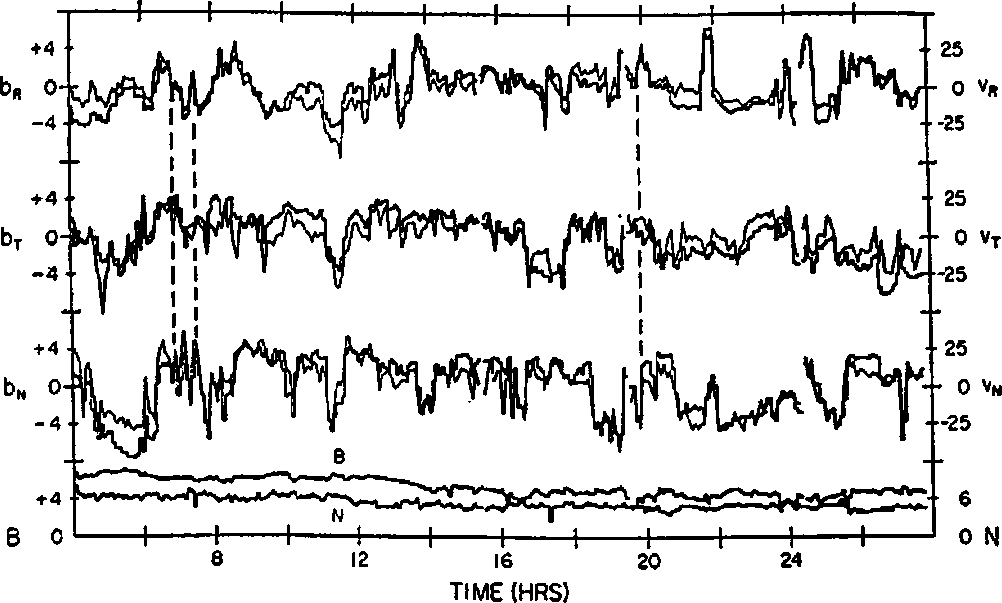
\includegraphics[width=0.7\columnwidth]{Fundamentos/fig3.png}
  \caption{Veintiocho horas de datos de plasma y de campo magnético,
    demostrando la presencia de ondas de Alfv\'en casi puras. Las seis
    curvas superiores corresponden a las componentes de las
    velocidades y del campo magnético, promediadas sobre el periodo de
    muestreo de la sonda. Los ejes verticales a la derecha
    corresponden a las componentes de la velocidad en km/seg ($R$ =
    radial, $T$ = tangencial, $N$ = normal, relativas al plano
    eclíptico); los ejes verticales a la izquierda corresponden a las
    componentes del campo magnético en nT. Las dos curvas inferiores
    corresponden a la fuerza del campo magnético y a la densidad
    numérica de protones (en cm$^{-3}$). Image extraída de
    \cite{belcher_large-amplitude_1971}.}
  \label{fig:equiparticion}
\end{figure}

Las simulaciones también tratan la cuestión del índice espectral en
MHD. Los espectros de energías obtenido por viejas simulaciones
computacionales de turbulencia MHD resultaron poco concluyentes. Por
ejemplo, simulaciones con resolución numérica de $180^3$ puntos de
grilla \cite{politano_current_1995} no pudieron generar un rango
inercial extendido. Simulaciones más recientes y con mayor resolución
\cite{biskamp_scaling_2000} proveyeron resultados que apoyan la ley de
Kolmogorov de los $-5/3$ (figura \ref{fig:normalizedspectrum}). El
espectro mostrado ha sido multiplicado por $k^{5/3}$, resultando así
en una región plana que indica un claramente discernible, aunque
pequeño, rango inercial $\tilde{E}(\tilde{k})\tilde{k}^{5/3} =
\tilde{k}^{5/3}E_K/\left(\epsilon\eta^5\right)^{1/5} = \tilde{C}_K
F(\tilde{k})$, donde $\tilde{C}_K$ es una constante y
$\tilde{k}=kl_d$, con $l_d=\left(\mu^3/\epsilon\right)^{1/4}$ la
escala de disipación de Kolmogorov (asumiendo $\mu=\nu$).

\begin{figure}[h]
  \centering
  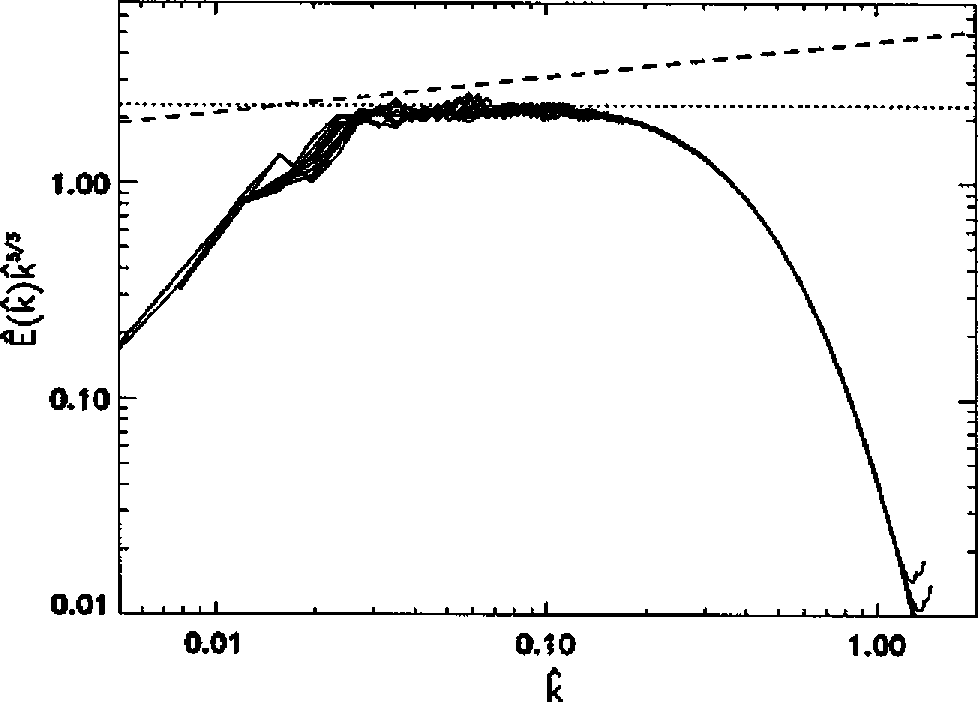
\includegraphics[width=0.7\columnwidth]{Fundamentos/fig4.png}
  \caption{Imagen del espectro normalizado, integrado en angularmente,
    en turbulencia MHD versus $\hat{k} = k\ell_d$ (donde $\ell_d$ es
    la escala de disipación de Kolmogorov). Todas las curvas dse
    encuentran multiplicadas por $k^{5/3}$. El escaleo de Kolmogorov
    se encuentra fuertemente sugerido por esta simulación numérica
    directa (curva sólida), con helicidad magnética nula. La línea
    discontinua indica el espectro $k^{-3/2}$ de Iroshnikov-Kraichnan
    (ver sección \ref{sec:escaleoI-K}), mientras que la línea punteada
    muestra el espectro de Kolmogorov, con $C_K = 2.3$. Imagen
    extraída de \cite{biskamp_scaling_2000}.}
  \label{fig:normalizedspectrum}
\end{figure}

Las hojas de corriente de pequeña escala son la característica
disipativa dominante en escalas pequeñas para turbulencia MHD, tanto
en tres dimensiones \cite{biskamp_scaling_2000} como en dos
\cite{matthaeus_turbulent_1986}. El rol crucial de la formación de
hojas de corriente y de reconexión debida a la turbulencia puede verse
\cite{dmitruk_coronal_2002} en modelos reducidos \textit{wave-driven}
de MHD que conceptualmente está entre el caso puramente 2D y el
puramente 3D. En 3D, las hojas de corriente están mucho más
distorsionadas, y encontrar los sitios de reconexión es más difícil
que en el caso 2D \cite{politano_current_1995}. La formación de hojas
de corriente asociadas con reconexión de estructuras magnéticas
cercanas es un aspecto fundamental de la turbulencia MHD, que está
relacionado con movimientos del tipo \textit{strain}.

La dinámica de las ondas de Alfvén, paralela al campo medio, no
controla la turbulencia, que en su lugar es gobernada por el
movimiento tipo \textit{eddies} perpendiculares al campo. Biskamp y
M\"uller argumentan que en tres dimensiones el movimiento arremolinado
puede dominar fácilmente la dinámica por sobre las ondas de Alfv\'en;
en consecuencia, el \textit{sweeping} aleatorio es más débil que el
\textit{straining} en turbulencia MHD 3D en ausencia de un campo
magnético DC. Esto a su vez indica que la transferencia de energía
local y las interacciones locales son dominantes.


\subsubsection{Cuando el \textit{sweeping} aleatorio es dominante:\\
  escaleo de Iroshnikov-Kraichnan}\label{sec:escaleoI-K} La forma más
simple de incorporar efectos de \textit{sweeping} es asumir isotropía
estadística, pero con la escala de tiempos de descorrelación
controlada por el periodo de una onda de Alfv\'en característica.  De
esta forma, Iroshnikov \cite{iroshnikov_turbulence_1964} y Kraichnan
\cite{kraichnan_inertial-range_1965} retuvieron las suposiciones
básicas de Kolmogorov de isotropía y localidad en el número de onda de
las interacciones no lineales. Las fluctuaciones de pequeña escala son
vistas como paquetes de onda de Alfv\'en viajando junto al campo
magnético y sufriendo breves ``colisiones'' con los paquetes de onda
propagándose en sentido opuesto. Específicamente, Iroshnikov y
Kraichnan sugirieron que las correlaciones triples de velocidades en
turbulencia MHD decaen en un tiempo del orden del periodo de una onda
de Alfv\'en. Entonces, $\tau_T = \tau_A$, $\tau_A = (V_A k)^{-1}$, y
$\epsilon = \tilde{C}^2 \tau_T(k) k^4 E^2(k)$. Como resultado, se
obtiene el conocido espectro $k^{-3/2}$ de Iroshnikov-Kraichnan.

Grappin \cite{grappin_alfvenic_1982} examinó las propiedades de la
cascada de Iroshnikov-Kraichnan utilizando la aproximación 3D de
\textit{EDQNM}. Encontró, luego de varios \textit{eddy turnover
  times}, un estado cuasiestacionario que exhibe un rango inercial que
escala como $-3/2$, con correlación nula entre el campo magnético y el
de velocidades. Simulaciones numéricas directas de 2D ofrecen soporte
a dicho escaleo \cite{biskamp_dynamics_1989, biskamp_geometric_1993,
  galtier_parametric_1999}. Biskamp y M\"uller
\cite{biskamp_scaling_2000} señalaron que en 2D, los movimientos
arremolinados son débiles, tal como manifiesta el espectro energético
empinado en tubulencia hidrodinámica 2D. Por lo tanto, el
\textit{straining} aparece debilitado, y el \textit{sweeping} inducido
por ondas de Alfv\'en domina los efectos de descorrelación.




\subsubsection{Fenomenología extendida}

Matthaeus y Zhou \cite{matthaeus_extended_1989, zhou_models_1990}
desarrollaron un marco en el cual ambas escalas temporales,
$\tau_{nl}$ y $\tau_A$, coexisten, de una forma análoga a la
composición del tiempo de correlación triple en la clausura
\textit{EDQNM} \cite{pouquet_strong_1976}. El punto es que el tiempo
de vida de las correlaciones de las transferencias $\tau_T(k)$ se
calcula más precisamente teniendo en cuenta las influencias de ambos
agentes externos y de las interacciones no lineales
turbulentas. Componiendo las tasas asociadas, obtenemos
\begin{equation}
  \frac{1}{\tau_T(\vec{k})} = \frac{1}{\tau_{nl}(\vec{k})} +
  \frac{1}{\tau_A(\vec{k})}.
\end{equation}
Notar que en general, pero dentro de la aproximación de transferencias
locales no lineales, el tiempo no lineal puede ser una función del
vector de onda $\vec{k}$. Esto se reduce a los casos límite esperados
cuando la fuerza del campo magnético efectivo tiende o bien a cero o
bien a infinito, por lo que $\tau_T$ se acerca a $\tau_{nl}$ o a
$\tau_A$, respectivamente. Acordemente, para el caso clásico de
turbulencia isotrópica, los espectros de energía, $E(k)\sim k^{-m}$,
tal como se muestra en la figura \ref{fig:Omnidirectional_vs_k}, tienen un exponente
de escaleo $3/2 \leq m \leq 5/3$, y se reduce a o bien la forma de
Iroshnikov-Kraichnan o bien la forma de Kolmogorov en el límite
apropiado.

\begin{figure}[h]
  \centering
  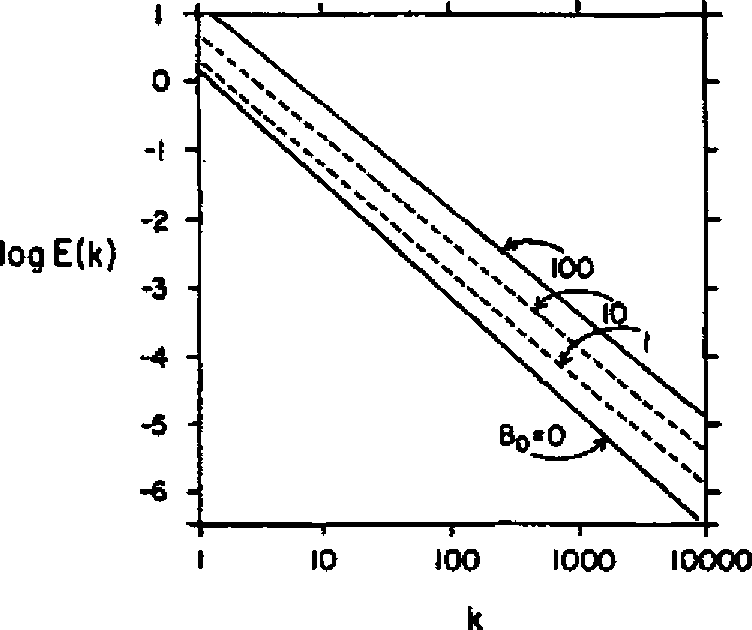
\includegraphics[width=0.7\columnwidth]{Fundamentos/fig7.png}
  \caption{Espectro energético onmidireccional versus número de onda,
    computado a partir de un espectro de energía generalizado
    \cite{matthaeus_extended_1989}. Se muestran cuatro valores de
    intensidad del campo magnético: $B_0 = 0$, $1$, $10$ y $100$. La
    pendiente se aplana y el nivel espectral se incrementea medida que
    la fuerza del campo aumenta, indicando una transición suave del
    escaleo $-5/3$ de Kolmogorov ($B_0 = 0$) a un escale a $B_0 = 100$
    que se acerca al $-3/2$ de Iroshnikov-Kraichnan. Extraída de
    \cite{matthaeus_extended_1989}.}
  \label{fig:Omnidirectional_vs_k}
\end{figure}



\subsection{MHD anisotrópico}
Kraichnan era conciente de que la presencia de un campo magnético de
gran escala que respalde la propagación de ondas de Alfv\'en puede
inducir una anisotropía  \cite{galtier_weak_2000}. En el caso de
Iroshnikov-Kraichnan, el \textit{sweeping} de Alfv\'en disminuye las
interacciones no lineales entre las fluctuaciones de Els\"asser
$z^\pm$, que aparecen simétricamente en la \cref{eq:MHDElsasser}. Un
campo magnético de gran escala suprime el crecimiento de gradientes
paralelos al campo magnético, pero como los gradientes perpendiculares
no se ven afectados, los efectos no lineales (\textit{strain})
continúan bombeando energía hacia las escalas más pequeñas, sólo que
anisotrópicamente. Bajo ciertas circunstancias, esto lleva a estados
cuasi-bidimensionales.

Cuando la turbulencia es suficientemente bidimensional, la escala
temporal de \textit{sweeping} debido a propagaciones paralelas al
campo $B_0$ deja de ser pequeña en comparación con los tiempos de
interacción de \textit{strainings} intrínsecos de las fluctuaciones, y
la dinámica de $z^+$ y $z^-$ se vuelve similar a la turbulencia MHD
bidimensional, por lo que resulta casi independiente de $B_0$
\cite{chen_inhibition_1997, hossain_phenomenology_1995}. Esto explica
por qué las conclusiones principales de las simulaciones MHD 3D con un
campo magnético externo impuesto \cite{oughton_influence_1994}, son
consistentes con los estudios bidimensionales
\cite{shebalin_anisotropy_1983}.

Entonces, es esperable que la estructura del espectro sea altamente
anisotrópica en la presencia de un campo DC, como fue originalmente
sugerido basándose en mediciones experimentales en el Culham Zeta
Device \cite{robinson_structure_1971}. El caso MHD bidimensional, el
cual no se ve afectado por la presencia de un campo DC perpendicular
fuerte, fue intensamente estudiado en la década del 70, y se sugirió
\cite{fyfe_high-beta_1976, fyfe_dissipative_1977} que el análisis de
Kolmogorov y su consiguiente escaleo de $-5/3$ sería aplicable al
rango inercial 2D asociado con una cascada de energía directa hacia
las escalas pequeñas. Este resultado estimuló el debate teórico, que
continuó durante más de 20 años.

A diferencia de caso 2D considerado por Fyfe
\cite{fyfe_dissipative_1977}, en el cual el campo DC define un plano
perpendicular, Shebalin \cite{shebalin_anisotropy_1983} estudió MHD 2D
en un plano que contiene al campo DC. Esto define una dirección
preferencial adicional, y la anisotropía puede desarrollarse en el
plano 2D. Las simulaciones 2D incompresibles de Shebalin
\cite{shebalin_anisotropy_1983} revelaron el desarrollo de una
anisotropía fuerte y distintiva: la energía se acumula
preferencialmente en los vectores de onda $\vec{k}$ perpendiculares a
$\vec{B}_0$. Oughton \cite{oughton_influence_1994} confirmó los
resultados de Shebalin en tres dimensiones encontrando que, con un
campo magnético DC, la transferencia de energía a modos
perpendiculares aumenta, comparativamente a los paralelos. Oughton
encontró que la anisotropía tiende a incrementarse con (i) la fuerza
del $B_0$ (con saturación a partir de $B_0 \geq 3b$); (ii) número de
onda $k$; (iii) número de Reynolds mecánico y magnético; (iv) tiempo
(con saturación dependiendo el número de Reynolds), y (v)
decrecimiento de la correlación cruzada.

La manifestación de anisotropía espectral en el espacio real es la
aparición de gradientes perpendiculares a la dirección media del campo
magnético, más intensos que los gradientes a lo largo del campo. Como
resultado, las longitudes de correlación son más largas a lo largo del
campo, y es esperable que las estructuras aparezcan elongadas en la
dirección de campo medio. Esta característica se encuentra ilustrada
en los resultados de las simulaciones numéricas de la figura
\ref{fig:currentdensity}.

\begin{figure}[h!]
  \centering
  \includegraphics[width=0.7\columnwidth]{Fundamentos/fig8.png}
  \caption{Mapas de color de la densidad de corriente $j_z$ en
    secciones transversales $x-y$ y $x-z$ de una simulación de
    turbulencia MHD 3D, con un campo magnético DC $B_0 \hat{z}$:
    arriba, $B_0 = 0$; al medio, $B_0/\delta B = 1$; abajo,
    $B_0/\delta B = 8$. Imagen extraída de
    \cite{zhou_colloquium_2004}}
  \label{fig:currentdensity}
\end{figure}


La anisotropía también es encontrada en la turbulencia del viento
solar. La evidencia para la anisotropía espectral del viento solar es,
hoy en día, indirecta; pero no obstante ha ganado un peso considerable
por las indicaciones consistentes de anisotropía provenientes de
diferentes tipos de estudios \cite{matthaeus_unquiet_1995}. Las
observaciones directas sugieren que las fluctuaciones del viento solar
son anisótropas \cite{carbone_model_1995} y que contienen una mezcla
de excitaciones en vectores de onda casi perpendiculares
\cite{bieber_dominant_1996}. Adicionalmente, el rango inercial del
viento solar admite una distintiva varianza anisotrópica, con una
varianza paralela inhibida. En las simulaciones, la aparición de esta
característica requiere baja compresibilidad
\cite{matthaeus_anisotropic_1996}.

Para ofrecer una interpretación simple y físicamente atractiva del
desarrollo de la anisotropía en la dirección perpendicular al campo
magnético DC aplicado, Shebalin \cite{shebalin_anisotropy_1983} apela
a un argumento de interacción resonante de tres ondas. Esta
interpretación se basa en una teoría de turbulencia débil
\cite{zakharov_kolmogorov_1992}, que sólo computa correciones de
primer orden a las soluciones de la ecuación lineal de MHD. En este
marco, los términos no lineales de las ecuaciones MHD cancelan
exactamente las soluciones de ondas, por lo que ondas propagándose en
la misma dirección no generan modos adicionales. Dos modos de Fourier
excitados pueden intercambiar energía eficientemente con un tercer
modo sólo si la tríada obedece la condición estándar de resonancia
\cite{montgomery_anisotropic_1995}: $\vec{k_1} + \vec{k_2} =
\vec{k_3}$, y $\omega(\vec{k_1}) - \omega(\vec{k_2}) = \pm
\omega(\vec{k_3})$. Aquí, $\vec{k_1}$ y $\vec{k_2}$ son vectores de
onda asociados a dos modos excitados de Fourier que están excitando
mediante resonancia un tercer vector de onda $\vec{k_3}$. En el límite
lineal, se asume que los tres modos tienen asociada una dependencia
temporal del tipo $\exp(-i\omega t)$, y satisfacen la relación
$\omega(\vec{k}) = \vec{k}\cdot\vec{V}_A$, donde $\vec{V}_A =
\vec{B}_0/(4\pi\rho)^{1/2}$ es el vector de velocidad de Alfv\'en
asociado al campo magnético medio. Las ondas interactuantes deben
propagarse en direcciones opuestas, que dan cuenta por el signo de
diferencia en el lado izquierdo de la condición para las
frecuencias. Las tríadas de ondas que satisfagan $\vec{k_1}\cdot
\vec{V}_A - \vec{k_2}\cdot \vec{V}_A = \pm \vec{k_3}\cdot \vec{V}_A$
tendrán acoplamiento no nulo sólo si $\vec{k_1}\cdot \vec{V}_A = 0$ ó
$\vec{k_2}\cdot \vec{V}_A = 0$. En consecuencia, $\vec{k_1}$ ó
$\vec{k_2}$ tendrán componente nula a lo largo de $\vec{B}_0$.

Las consecuencias físicas de los acoplamientos de tres ondas puede
resumirse de la siguiente manera: al orden principal, no hay
transferencia para un campo magnético DC impuesto; la transferencia en
la dirección perpendicular no es impedida por el acoplamiento de ondas
de Alfv\'en que suprime la transferencia paralela; consecuentemente,
la transferencia MHD perpendicular se realiza de manera muy similar al
caso MHD 2D \cite{fyfe_dissipative_1977}. De esta manera, es esperable
un espectro $k_\perp^{-5/3}$ para los vectores de onda
perpendicular. En la dirección paralela, se produce una transferencia
débil, pero por cada paso en $k_\parallel$, mucha energía es desviada
a $k_\perp$ más grandes. En consecuencia, es esperable que el espectro
paralelo sea una exponencial $\sim \exp(-k_\parallel)$. La primera
sugerencia de esto la planteó Montgomery
\cite{montgomery_density_1987}.

Aunque la justificación física para la ocurrencia de la anisotropía
espectral haya sido dada en el espacio de números de onda, es
esperable que este fenómero tenga una manifestación en el espacio real
con algún grado de localidad. Un campo magnético de escala
suficientemente grande debería inducir efectos locales que sean
indistinguibles de un campo DC estrictamente uniforme. En
consecuencia, sería esperable poder entender la ocurrencia de
anisotropías enteramente en el contexto de un sistema teniendo
corrientes eléctricas localizadas y campos magnéticos con escala
estrictamente finita. Hay mucho estudios numéricos
\cite{cho_anisotropy_2000, milano_local_2001} que se encargan de este
problema, y concluyen que la anisotropía descripta posee efectivamente
un análogo puramente local. El punto básico vuelve a las mediciones en
el Culham Zeta Device de Robinson y Rusbridge
\cite{robinson_structure_1971}, que encontraron que la correlación de
las fluctuaciones magnéticas caen mucho más rápidamente en las
direcciones perpendiculares a un campo aplicado de gran escala, que
respecto de la dirección paralela. Aplicaciones de estas ideas a datos
simulados indican que la anisotropía efectivamente ocurre en forma
local. Las correlaciones caen más rápidamente en las direcciones
transversales al campo magnético medio calculado localmente. La
anisotropía resulta ser más grande a escalas pequeñas
\cite{cho_anisotropy_2000} y mayor donde la fuerza del campo medio
local es mayor.



%%% Mininni
\subsection{Localidad de las interacciones a partir de las transferencias \emph{shell-to-shell}}
En los últimos años, el aumento de la potencia de las computadoras ha
permitido la exploración numérica de turbulencia MHD en diferentes
regímenes. Además, los estudios de transferencia energética
\textit{shell-to-shell} \cite{alexakis_shell_2005, dar_energy_2001,
  debliquy_energy_2005} han permitido el cálculo explícito de las
interacciones de escala en la turbulencia de MHD utilizando el
resultado derivado de las simulaciones y sin la necesidad de calcular
las interacciones triádicas más complejas.

En líneas generales, las transferencias \textit{shell-to-shell}
$T_{uw}(Q, K)$ permiten analizar la transferencia energética
entre dos campos $\vec{v}$ y $\vec{w}$ (que pueden ser $\vec{u}$,
$\vec{b}$, $\vec{z^+}$ o $\vec{z^-}$), entre dos cascarones $Q$ y $K$
\cite{mininni_scale_2011}.

Los resultados obtenidos indican, en todos los casos, que las
transferencias $T_{uu}$ y $T_{bb}$ tienen un comportamiento local: la
energía es transferida a escalas vecinas más pequeñas, de una forma
similar a la turbulencia hidrodinámica \cite{alexakis_imprint_2005,
  mininni_large_2006}. En cambio, $T_{ub}$ y $T_{bu}$, que expresan el
intercambio de energía entre los campos magnético y de velocidades,
han tenido comportamientos variados, dependiendo del problema
estudiado.

En el caso de turbulencia homogénea e isotrópica, con forzado sólo
mecánico, Alexakis, Mininni y Pouquet \cite{alexakis_imprint_2005}
encontraron una pequeña pero no despreciable transferencia no
local. Los resultados pueden observarse en la
\cref{fig:transferfunctions}. En dicha figura se puede observar las
funciones de transferencia típicas del caso. Se puede ver que tanto
$T_{uu}$ como $T_{bb}$ son locales, con un pico negativo para $K<Q$ y
uno positivo para $K>Q$, que indica que la energía es removida de las
escalas con números de onda vecinos más chicos y transferida hacia los
estados con números de onda vecinos más grandes. También se puede
observar que para $T_{ub}$ (transferencia de energía mecánica a
magnética) el comportamiento es distinto. En este caso, el flujo a
gran escala inyecta energía (a través del \textit{straining})
directamente en el campo magnético a todas las escalas. Esto se
manifiesta como un pico en la escala de fuerza mecánica para todos los
valores de $Q$, y como una meseta positiva que se extiende hasta
$K\approx Q$.  En otras palabras, en una capa $K$ dada, el campo
magnético recibe energía del campo de velocidad en todas las capas con
$Q<K$, y da energía al campo de velocidad en las capas con $Q>K$. Este
resultado se puede interpretar como sustento del campo magnético
contra la disipación Ohmica por acción de un dínamo: para mantener el
campo magnético cuando sólo se excita el campo de velocidad, es
necesario un flujo no nulo de energía desde el campo de velocidad
hacia el campo magnético, en todo momento. No obstante, cabe señalar
que a pesar de la importancia que cumple este efecto, en el estado
estacionario esta transferencia no local es pequeña en comparación con
las transferencias locales, representando alrededor de un $10\%$ ó
$20\%$ en las resoluciones estudiadas \cite{mininni_large_2006}. Al
considerar las variables de Els\"asser, se observó que las funciones
de transferencia se volvían más locales aún.
\begin{figure}[h!]
  \centering
  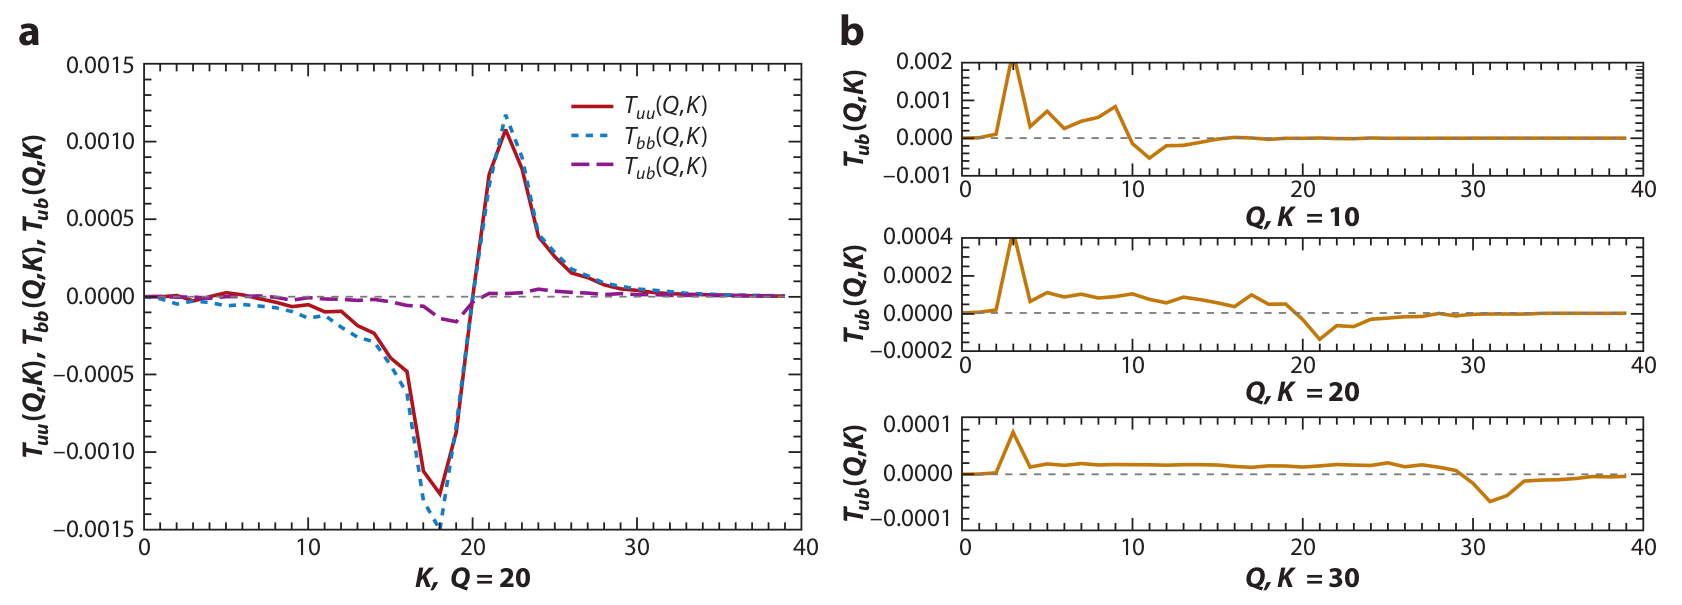
\includegraphics[width=0.99\columnwidth]{Fundamentos/figtransferfunctions.png}
  \caption{(a) Funciones de transferencia para turbulencia MHD forzada
    mecánicamente, para el cascarón $Q = 20$. Las funciones $T_{uu}$ y
    $T_{bb}$ son locales, con un pico negativo para $K<Q$ y uno
    positivo para $K>Q$, que indica que la energía es removida de los
    números de onda vecinos más chicos y transferida hacia los números
    de onda vecinos más grandes. La transferencia energética desde el
    campo magnético al cinético en mucho más pequeña en amplitud, y
    también resulta local. (b) Función de transferencia $T_{ub}$
    (mecánica a magnética), para distintos valores de $K$. Esta
    función es no local, con un pico alto en la escala del forzado y
    con un \emph{plateau} constante y positivo que se extiende hasta
    $K\approx Q$. Figura adaptada de \cite{alexakis_imprint_2005}.}
  \label{fig:transferfunctions}
\end{figure}


Otro caso estudiado corresponde al decaimiento turbulento libre, donde
los efectos no locales son despreciables
\cite{debliquy_energy_2005}. Es este caso, tanto $T_{uu}$ y $T_{bb}$,
como $T_{ub}$ y $T_{bu}$, resultan locales y de transferencia de
grandes escalas a pequeñas. Se obtuvieron resultados similares en
observaciones del viento solar \cite{bruno_solar_2005}. Las
diferencias entre los casos de decaimiento forzado y libre pueden
entenderse al notar que, en los recorridos forzados mecánicamente, el
campo de velocidad debe suministrar energía continuamente al campo
magnético para sostenerlo contra la disipación Ohmica. Este no es
necesariamente el caso de las corridas en decaimiento libre, en las
que ambos campos se disipan en el tiempo.

Por último, el caso anisotrópico resulta más complejo. Por lo pronto,
no resulta tan evidente cómo tomar las distintas capas. Una
posibilidad es introducir funcioner de transferencia
\textit{shell-to-shell} tomando como capas secciones cilíndricas
(asociados con el número de onda $k_\perp$ perpendicular al campo
magnético medio) y secciones planas (asociadas a los
$k_\parallel$). Las funciones de transferencia para las energías de
Els\"asser fueron locales en las dos direcciones, independientemente
de la amplitud del campo magnético externo. Sin embargo, las
interacciones entre las ondas de Alfv\'en contrapropagantes resultaron
ser no locales. Para campos magnéticos fuertes, la mayor parte del
flujo de energía en la dirección perpendicular fue resultado de
interacciones con modos con $k_\parallel = 0$
(\cref{fig:mininnianisotropo}). Sin embargo, en la dirección
paralela, los modos $k_\parallel = 0$ no pueden transferir energía, y
se observó que la mayoría de las interacciones tienen lugar con modos
cercanos a $k \approx 0$. Los resultados están en acuerdo cualitativo
con las predicciones de la teoría de la turbulencia débil
\cite{galtier_weak_2000} y con algunos modelos fenomenológicos no
locales \cite{alexakis_nonlocal_2007}.
\begin{figure}[h!]
  \centering
  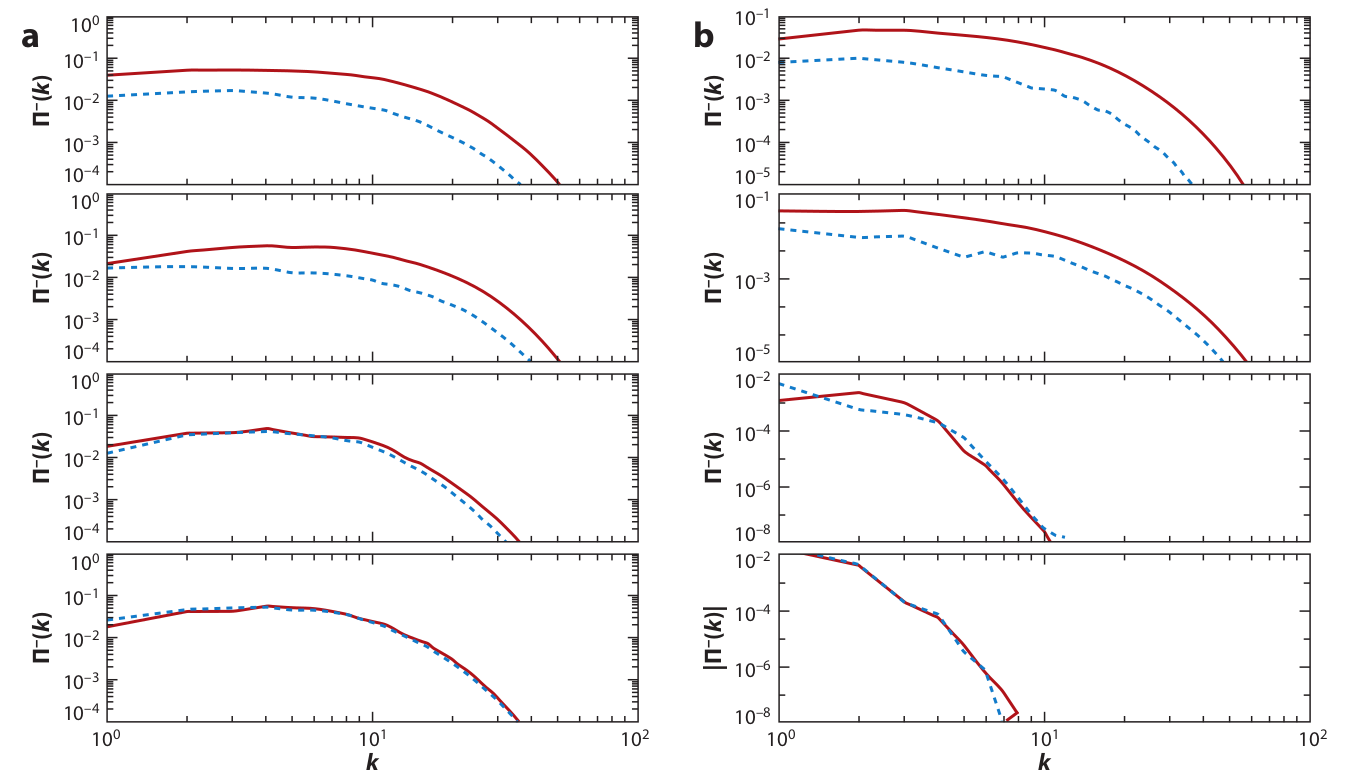
\includegraphics[width=0.99\columnwidth]{Fundamentos/figmininnianisotropo.png}
  \caption{(a) Flujo de energía total (líneas rojas continuas) a
    través de cilindros y flujo parcial asociado con interacciones con
    modos con $k_\parallel = 0$ (líneas azules discontinuas), con
    cuatro valores diferentes del campo magnético externo $B_0$, desde
    $0$ hasta $15$ (desde arriba hacia abajo). (b) Igual que en el
    panel \emph{a}, pero con el flujo total y el flujo parcial
    asociados con interacciones con modos con $k_\parallel = 1$ a
    través de planos. Figura adaptada de
    \cite{alexakis_anisotropic_2007}.}
  \label{fig:mininnianisotropo}
\end{figure}

Las consideraciones anteriores llevaron a varios autores a considerar
si algunos de los supuestos habituales en la turbulencia hidrodinámica
se mantenían efectivamente en el caso de MHD. A partir de análisis de
la transferencia de capa a capa, el escenario más realista para la
energía está representado en la \cref{fig:transferfunctionsMHD}: las
interacciones entre los mismos campos son en su mayoría locales, y las
interacciones entre la velocidad y el campo magnético pueden tener
diferentes grados de no localidad dependiendo de si la turbulencia es
forzada o decae libremente, dependiendo de cómo se mantengan la
velocidad y los campos magnéticos contra la disipación en el caso
forzado, y dependiendo de la presencia de un campo magnético
externo. Actualmente no está claro si el grado variable de no
localidad con la configuración convergerá en una solución universal
para números de Reynolds muy grandes.
\begin{figure}[h!]
  \centering
  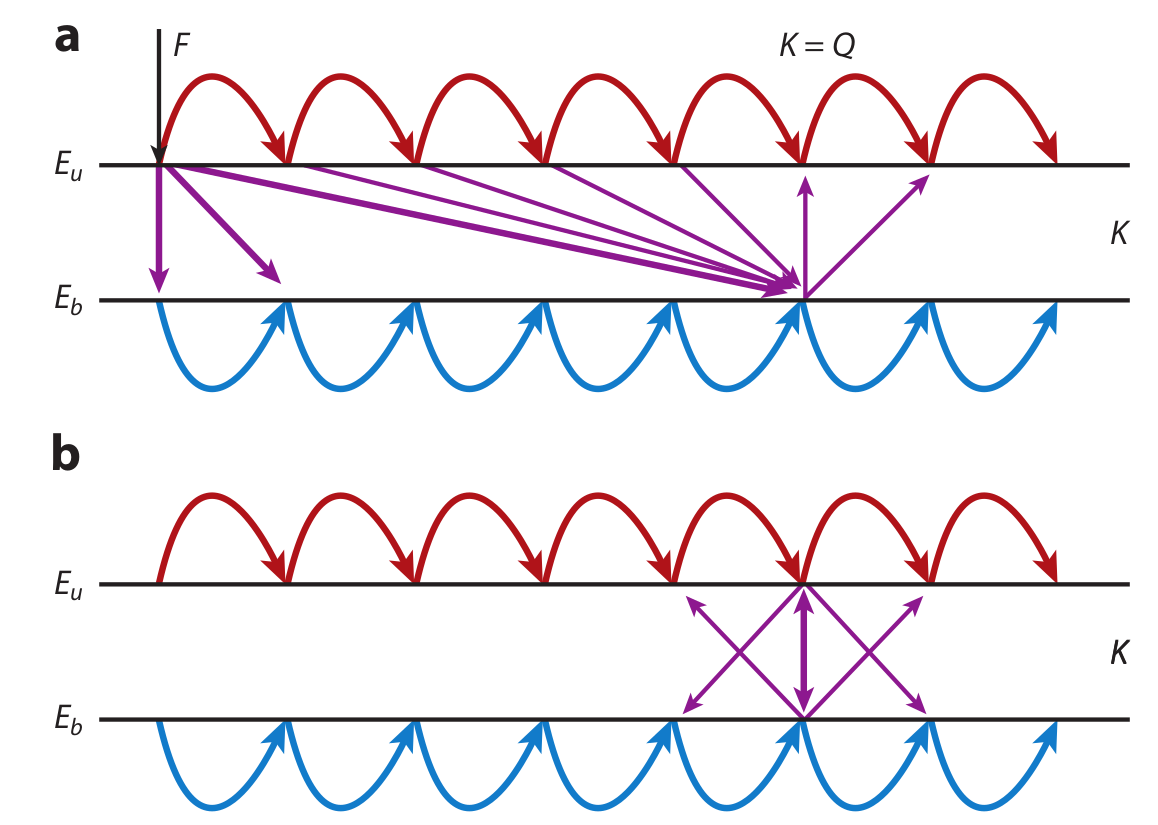
\includegraphics[width=0.7\columnwidth]{Fundamentos/figtransferfunctionsMHD.png}
  \caption{Diagrama de las diversas transferencias de energía
    \emph{shell-to-shell} identificadas en simulaciones de turbulencia
    MHD isotrópica y homogénea. Las transferencias de $T_{uu}$ se
    muestran en rojo, las transferencias de $T_{bb}$ en azul y las de
    $T_{ub}$ y $T_{bu}$ en violeta. El grosor de las flechas indica
    aproximadamente la fuerza de las transferencias. (a) Simulaciones
    forzadas mecánicamente. En la capa $K$, el campo magnético recibe
    energía del campo de velocidad en todas las escalas más grandes y
    le da energía al campo de velocidad en escalas ligeramente más
    pequeñas. (b) Turbulencia en decaimiento libre. $T_{ub}$ y
    $T_{bu}$ transfieren energía sólo localmente. En ambos casos, las
    transferencias $T_{uu}$ y $T_{bb}$ son locales y dan la mayor
    contribución al flujo.}
  \label{fig:transferfunctionsMHD}
\end{figure}

En cualquier caso, existe un consenso cada vez mayor de que la
turbulencia de MHD es menos local que la turbulencia hidrodinámica,
aunque no es claro en qué medida. Por el momento, no está claro si
estos efectos desaparecerán para un mayor número de Reynolds; tampoco
está claro, en caso de permanecer, qué impacto tendrán en la dinámica
del flujo y en qué condiciones. Sin embargo, los diferentes grados de
no localidad observados en las resoluciones actuales, y la existencia
de procesos no locales en MHD (como, por ejemplo, el dínamo a pequeña
escala), requieren una discusión sobre la validez de la hipótesis de
localidad de interacciones, y si existe un solo tipo de turbulencia
MHD o muchos. Estos son puntos a tener en cuenta al realizar un
análisis fenomenológico o teórico.


%%% END Mininni


\section{Discusión y conclusiones}\label{sec:conclusiones}

Con la base de las propiedades física discutidas, es posible
desarrollar una metodología para estimar los espectros de energía y
las funciones de correlación en varios regímenes de turbulencia
MHD. La idea es la siguiente: se estima una escala de tiempo del
espectro de transferencia, incorporando efectos debidos tanto a los
movimientos no lineales de \textit{straining} como a la influencia
tipo \textit{sweeping} de la propagación de ondas. La influencia
relativa de estos efectos será relacionada con grado y tipo de
anisotropía esperada; por ejemplo, si la anisotropía se debe a un
campo magnético DC externo fuerte o si se debe a campo magnético
local. Acordemente, la transferencia espectral es o bien isotrópa,
cuando se toman en consideración grandes muestras de plasma, o bien es
anisótropa, cuando hay un campo magnético fuerte en las escalas
grandes. Con esta base, podemos examinar la tasa estacionaria de
transferencia de energía fenomenológicamente, haciendo uso de la
afirmación
\begin{equation}
  \epsilon = \Pi(k) = \tau_T(k) \frac{kE(k)}{\tau_{nl}^2},
\end{equation}
que es no es más que la \cref{eq:TR_sw}. En esta ecuación se
relacionan varios elementos físicos de la MHD:
\begin{itemize}
\item La transferencia de energía debe ser proporcional al tiempo de
  vida de la correlación triple, como en la \cref{eq:transferRate}.
\item La fuerza de las interacciones no lineales es medida por el
  \textit{eddy turnover} o la escala temporal no lineal, como en
  la \cref{eq:tauNL}.
\item Finalmente, el flujo espectral de energía debe ser definido de
  una forma (\cref{eq:TR_sw}) que sea compatible con los ítems
  anteriores. Esta es más que una relación formal, y de hecho puede
  ser utilizada para hacer estimaciones de la forma del espectro en
  una variedad de casos físicos interesantes.
\end{itemize}

Este procedimiento nos permite fácilmente entender la física de las
teorías de Kolmogorov y de Iroshnikov-Kraichnan, así como sus
diferencias. Además, no se requieren teorías de clausura complejas o
esquemas de perturbaciones. Si, en adición, queremos desarrollar
aproximaciones para las funciones de correlación tiempo-dependientes,
como las funciones de correlación Eulerianas (un punto espacial, dos
temporales), o las descorrelaciones de dos tiempos que aparecen en las
teorías de clausura, deberíamos proceder de una manera análoga:
adoptamos una forma funcional razonable para la funcion de correlación
temporal, dependiente de una única escala temporal, digamos,
del mismo tiempo de transferencia espectral.

En este trabajo hemos intentado dar un panorama del rol influente de
distintas escalas temporales para establecer la transferencia de
energía, las cascadas, la no localidad y la anisotropía, en
turbulencia MHD. Como en el caso hidrodinámico, la escala temporal
``nativa'' puede dividirse en movimientos de \textit{straining}
debidos a la propia distorsión de los \textit{eddies}, y a movimientos
de \textit{sweeping} que desplazan estructuras de pequeña escala bajo
la influencia de los campos de gran escala. En MHD, como en
hidrodinámica, los movimientos de \textit{straining} son
dominantemente locales en escala, en la que las distorsiones no
lineales son más efectivas para interacciones entre \textit{eddies} de
aproximadamente el mismo tamaño. En MHD, no obstante, los movimientos
tipo \textit{sweeping} son más complejos que en hidrodinámica debido
al efecto de propagación de Alfv\'en. El \textit{sweeping} Alfv\'enico
indroduce un nuevo nivel de no-localidad en MHD y una fuerte tendencia
a que la transferencia espectral ocurra anisotrópicamente respecto de
la dirección del campo magnético.

En el pasado se han hecho muchas diferencia entre los espectros de
Kolmogorov y de Iroshnikov-Kraichnan, y ambas posibilidades suelen ser
comparadas en simulaciones y en observaciones interplanetarias, con el
aparente objetivo de plantear una distinción firme entre estas
posibilidades. En esta propuesta, en la que el principal efecto que
variamos es la escala temporal para el decaimiento de las funciones de
correlación de transferencia, enfatizamos que en turbulencia MHD hay
una variación suave entre esos límites. La observación de varios
índices espectrales en varios casos es un indicativo del aumento de
los efectos de \textit{sweeping} respecto de los efectos de \textit{straining}, o de los
efectos locales respecto de los no locales, de acuerdo a cómo las
condiciones prevalecientes impacten en la relevancia de las escalas
temporales. La anisotropía es controlada por variación del tiempo de
descorrelación Alfv\'enico en comparación a la escala temporal local
no-lineal. Esto abre a un amplio rango de posibilidades para el
espectro anisotrópico y para los índices espectrales que puede
aparecer en MHD.

Como discutimos, se espera un empalme suave entre Kolmogorov e
Iroshnikov-Kraichnan en el caso de turbulencia MHD isotrópico, al
cambiar el cociente entre el tiempo de Alfv\'en y el tiempo
no-lineal. La proporción es también dependiente del número de onda, y
la descorrelación más tipo ondular suele ocurrir a escalas más
pequeñas. Con un campo magnético uniforme fuerte, el espectro
energético anisotrópico resultante puede reducierse a $k_\perp^{-5/3}$
cuando las interacciones resonantes y el \textit{strain}
cuasi-bidimensional es el efecto de descorrelación dominante, o a
$k_\perp^{-3/2}$ cuando la descorrelación Alfv\'enica cuasi-2D de gran
escala es fuerte. Cuando los efectos cuasi-2D son débiles, el espectro
puede convertirse tanto en $k_\perp^{-2}$ (turbulencia ``débil''),
cuando las interacciones locales son dominantes, o en $k_\perp^{-3}$,
cuando las interacciones no locales son dominantes. Cuando tanto las
interacciones locales como las no locales están presentes, el espectro
varía suavemente entre estos límites.

Consideraciones similares de las escalas temporales nos permiten
acercarnos a un modelado de las funciones de correlación Eulerianas
que aparecen en MHD.

Debe hacerse notar que la evidencia tanto observacional como de
simulaciones sólo ha identificado y analizado algunos de los regímenes
MHD que se han discutido, y es necesario estudiar más exhaustivamente
los regímenes de los parámetros MHD, incluyendo un amplio rango del
número de Reynolds, helicidad cruzada, anisotropía muy fuerte,
transición entre transferencia espectral local y no local, MHD que se
aleja considerablemente de equipartición entre energías cinética y
magnética, y la influencia de varios posibles efectos de disipación
cinética. La disponibilidad de varias escalas temporales hace que la
turbulencia MHD sea más compleja y multifacética que su contraparte
hidrodinámica, haciendo que probablemente permanezca como un área de
estudio activa.


\chapter[Paper1]{Paper1}
\label{ch:P1}
Recapitulando, en la aproximación lineal, las ecuaciones MHD permiten
la presencia de ondas Alfv\'en. El caso más simple corresponde a MHD
incompresible con un campo magnético de fondo uniforme $\vec{B}_0$,
para el cual la relación de dispersión lineal (en el caso ideal no
disipativo) describe ondas con frecuencia $ \omega =
\vec{k}\cdot\vec{V}_A$, para el número de onda $\vec{k}$, velocidad de
Alfv\'en $\vec{V}_A = \vec{B}_0 / \sqrt{4\pi\rho}$, y densidad
$\rho$. Además, las componentes de Fourier complejas de la velocidad
$\vec{v}(\vec{k})$ y de las fluctuaciones del campo magnético
$\vec{b}(\vec{k})$ son transversales al vector de onda, es decir,
$\vec{v}(\vec{k}) \cdot \vec{k} = \vec{b}(\vec{k}) \cdot \vec{k} =
0$. Curiosamente, estas ondas cuando se consideran de forma aislada
son soluciones no lineales exactas de las ecuaciones MHD.

Sin embargo, cuando se tienen en cuenta los términos no lineales, el
sistema también puede desarrollarse lejos de la dinámica de
equilibrio, con las ondas coexistiendo con remolinos en un flujo
turbulento completamente desarrollado [\cite{dmitruk_waves_2009}].  En
este régimen turbulento, no es necesariamente esperable una relación
directa o explícita entre la frecuencia y el número de onda, tal como
una relación de dispersión de las ondas.  Este régimen está
caracterizado por interacciones de distintos tipos, tales como
distorsiones no lineales, locales en escala, de los \textit{eddies}
[\cite{monin_statistical_2013, kolmogorov_local_1941,
    mccomb_physics_1992}], y efectos no locales
[\cite{alexakis_turbulent_2007, alexakis_anisotropic_2007,
    teaca_energy_2009, mininni_scale_2011}], donde el más extremo es
el \textit{sweeping} de las pequeñas escalas por los grandes
\textit{eddies} [\cite{kraichnan_structure_1959,
    tennekes_eulerian_1975, chen_sweeping_1989, nelkin_time_1990}].
Como ya vimos, para turbulencia MHD [\cite{pouquet_strong_1976,
    zhou_magnetohydrodynamic_2004}], adicionalmente al tiempo no
lineal global $\tau_{nl}$, hay también otras escalas temporales
asociadas a efectos no lineales dependientes de escala (local),
\textit{sweeping} y propagación de ondas.

%% {\color{purple} Al comienzo de la década de 1970, la investigación de la turbulencia
%% hidrodinámica se dirigió al estudio del tiempo de descorrelación del
%% campo de velocidades [\cite{orszag_numerical_1972,
%% orszag_analytical_1970, tennekes_eulerian_1975, heisenberg_zur_1948,
%% comte-bellot_simple_1971}]. La conclusión principal fue que el
%% \textit{sweeping} domina la descorrelación temporal en el rango
%% inercial [\cite{zhou_non-gaussian_1993,sanada_random_1992}].
%% Recientemente, se realizó un estudio similar para magnetohidrodinámica
%% [\cite{servidio_time_2011, matthaeus_eulerian_2010,
%% carbone_anisotropy_2011}]. Una diferencia con el caso hidrodinámico es
%% la presencia de otros fenómenos no locales (además del barrido), como
%% la propagación Alfv\'enica o la distorsión Alfv\'enica, a saber, el
%% ``barrido magnético''. El resultado principal de 
%% \cite{servidio_time_2011} respecto de la descorrelación temporal para
%% turbulencia isotrópica fue que, como en hidrodinámica, la
%% descorrelación temporal en MHD es gobernada por interacciones no
%% locales (en este caso, \textit{sweeping} y descorrelación de
%% Alfv\'en). Sin embargo, no pudieron distinguir entre los efectos del
%% \textit{sweeping} y de la distorsión Alfv\'enica.} MOVIDO A \cref{sec2:SpectraFreq}

En este capítulo, nuestro objetivo será profundizar el análisis
iniciado por \cite{servidio_time_2011} (ver
sección \ref{sec2:SpectraFreq}) y generalizarlo a plasmas magnetizados
a grandes escalas, donde la aproximación MHD resulta válida. Para
ello, estudiaremos los diferentes tiempos de correlación que aparecen
para las distintas escalas en el rango inercial de turbulencia MHD con
un campo guía. El objetivo principal será entender la descorrelación
temporal de las fluctuaciones, estudiando el valor relativo de los
tiempos de descorrelación para diferentes escalas. Así, seremos
capaces de relacionar las leyes de escalas de los tiempos de
descorrelación con la contribución de los diferentes efectos físicos:
distorsión no lineal, \textit{sweeping} aleatorio y propagación de
ondas de Alfv\'en. En otras palabras, estudiaremos la memoria
característica para cada escala espacial, a fin de identificar los
mecanismos de descorrelación temporal y observar si son locales o
no. Con este objetivo, consideraremos las fluctuaciones a más de una
escala espacial, para discernir entre los diferentes fenómenos
asociados con la descorrelación temporal, en particular la propagación
de ondas de Alf\'en y el \textit{sweeping} aleatorio.  Este método,
basado en el cómputo de espectros espacio-temporales y en las
funciones de correlación, fue propuesto e implementado en fluidos
rotantes por
\cite{clark_di_leoni_quantification_2014} (ver también
\cite{clark_di_leoni_spatio-temporal_2015} para una descripción
general del método). Meyrand y Galtier recientemente utilizaron el
espectro espacio-temporal para estudiar la transición de turbulencia
débil a turbulencia fuerte en MHD [\cite{meyrand_direct_2016}], y la
intermitencia en turbulencia MHD débil
[\cite{meyrand_weak_2015}]. Aquí consideramos el régimen de
turbulencia fuerte, y computamos tanto los espectros como los tiempos
de descorrelación.

La estructura del capítulo será la siguiente. En
la sección \ref{sec3:EqNumSim} introduciremos las ecuaciones y los métodos
numéricos empleados, así como también una descripción del espectro
espacio-temporal y de las funciones de correlación. Luego, en
la sección \ref{sec3:Res} presentaremos los resultados. Finalmente, la
discusión y las conclusiones serán expuestas en
la sección \ref{sec3:Conclusions}.

%%%%%%%%%%%%%%%%%%%%%%%%%%%%%%%%%%%%%%%%%
\section{Ecuaciones y simulaciones numéricas}\label{sec3:EqNumSim}

\subsection{Las ecuaciones MHD}\label{sec3:eq}

Las \cref{eq2:NS-MHDv,eq2:NS-MHDB} de MHD incompresible pueden
adimensionalizarse, obteniendo
\begin{equation}\label{eq3:MHD_v}
  \frac {\partial \vec{v}}{\partial t} +
  \vec{v }\cdot \nabla \vec{v} = -\frac{1}{\rho}\nabla p +
  \vec{j} \times \vec{B} + \frac{1}{R} \nabla^2\vec{v} + \vec{F}_v,
\end{equation}
\begin{equation}\label{eq3:MHD_b}
  \frac{\partial \vec{b}}{\partial t} = \nabla \times (\vec{v} \times \vec{B})
  + \frac{1}{R_m} \nabla^2 \vec{b} + \vec{F}_b,
\end{equation}
donde $\vec{v}$ es la velocidad del plasma; $\vec{B} = \vec{b}
+ \vec{B}_0$ el campo magnético, con una parte fluctuante $\vec{b}$ y
un campo medio DC $\vec{B_0}=B_0\hat{x}$; $\vec{j}
= \nabla \times \vec{b}$ la densidad de corriente; $p$ la presión,
$\rho$ la densidad del plasma, y $\vec{F}_v$ y $\vec{F}_b$ términos de
forzado que luego serán discutidos con más detalles. Las unidades se
basan en una velocidad característica $v_0$, que para MHD se toma como
la velocidad de Alfvén típica de las fluctuaciones del campo
magnético, $v_0 = \sqrt{\langle b^2 \rangle /(4\pi\rho)}$, con
$\langle . \rangle$ el promedio espacial. Los parámetros
adimensionales que aparecen en las ecuaciones son los números de
Reynolds cinético y magnético, es decir $R=v_0 L/\nu$ y $R_m = v_0 L
/\mu$, respectivamente, con $\nu$ la viscosidad cinemática, $\mu$ la
difusividad magnética y $L$ una escala de longitudes característica
(la caja de la simulación tiene un tamaño dado de $2\pi L$). La unidad
temporal es $t_0 = L/v_0$, que para MHD se convierte en el tiempo de
cruce Alfv\'enico (\emph{Alfv\'en crossing time}) basado en las
fluctuaciones del campo magnético.


\subsection{Espectros y funciones de correlación}\label{sec3:Wfspectrum_and_Gamma}

A partir de las ecuaciones \cref{eq3:MHD_v,eq3:MHD_b} y argumentos de
escala, es posible estimar los diferentes tiempos característicos. El
tiempo de los \textit{eddy turnover} locales puede ser definido como
$\tau_{nl} \sim \left[ k v(k) \right]^{-1}$, donde $k$ es el número de
onda y $v(k)$, la amplitud de la velocidad debido a las fluctuaciones
a escala $\sim 1/k$. Para una predicción del escaleo de velocidades
tipo Kolmogorov, $v \sim v_{rms} \left(kL\right)^{-1/3}$, las escalas
de tiempo no lineal en el rango inercial pueden ser escritas
aproximadamente como
\begin{equation}
\tau_{nl} = C_{nl} \left [
   v_{rms} L^{-1/3} \left(\sqrt{k^2_\perp +
   k^2_\parallel}\right)^{2/3}\right ]^{-1},
\label{eq3:taunl}
\end{equation}
donde $C_{nl}$ es una constante adimensional del orden de la
unidad (para una discusión más detallada,
ver \cite{zhou_magnetohydrodynamic_2004}). En lo que sigue, $v_{rms}
= \left\langle |\vec{v}|^2 \right\rangle ^{1/2}$ es una cantidad
global, típicamente dominada por las contribuciones de las grandes
escalas.

La física de la descorrelación temporal depende de otros efectos y,
por lo tanto, de otras escalas de tiempo MHD disponibles. Un ejemplo
es el tiempo característico de barrido a escala $\sim 1/k$, que puede
expresarse como
\begin{equation}
\tau_{sw} = C_{sw} \left( v_{rms}\sqrt{k^2_\perp + k^2_\parallel}
    \right)^{-1}.
\label{eq3:tausw}
\end{equation}
Este tiempo corresponde a la advección
de estructuras a pequeña escala por el flujo a gran
escala. Análogamente, se puede definir un tiempo de Alfvén
característico como
\begin{equation}
\tau_A= C_A \left( v_A k_\parallel \right)^{-1}.
\label{eq3:taua}
\end{equation}
Aquí, $C_{sw} $ y $C_A$ son otras constantes adimensionales del
orden de la unidad. Todas estas escalas de tiempo dependen del vector
de onda, y suponiendo que la escala de tiempo más corta domina la
dinámica, se pueden definir diferentes regiones en el espacio
$\vec{k}$ en el espectro de energía.

Las estadísticas de, por ejemplo, el campo magnético, puede ser
caracterizado por la función de correlación a dos puntos
espacio-temporal
\begin{equation}
R(\vec{r},\tau) = \left\langle \vec{b}( \vec{x},t) \cdot
  \vec{b}( \vec{x} + \vec{r},t+\tau) \right\rangle / \left\langle {\bf
    b}^2 \right\rangle.
\label{eq3:Rbij}
\end{equation}
Notar que esta expresión contiene tanto el espectro de energía como el
espectro de frecuencia Euleriano (teorema de Wiener-Khinchin); sin
embargo, contiene mucha más información que nos permite hacer un
análisis más sutil de las relaciones espacio-temporales.
Transformando Fourier en $r$, obtenemos una densidad espectral
retrasada temporalmente, que puede a su vez factorizarse como
$S(\vec{k},\tau) = S(\vec{k})\Gamma(\vec{k},t)$, donde $\vec{k}$ es el
vector de onda. La función $\Gamma(\vec{k},\tau)$, la función de
correlación dependiente de la escala [\cite{heisenberg_zur_1948,
comte-bellot_simple_1971, orszag_numerical_1972}], representa los
efectos dinámicos de descorrelación que describen la descorrelación de
tiempo de cada modo espacial $\vec{k}$.

Entonces, la función $\Gamma(\vec{k},\tau)$ es la función de
correlación temporal del modo de Fourier $\vec{k}$. Usando esto,
seremos capaces de identificar el tiempo de descorrelación
característico para cada modo $\vec{k}$, y en consecuencia la pérdida
de memoria de las fluctuaciones 3D cuyas longitudes características
sean de orden $k_x^{-1}$, $k_y^{-1}$ y $k_z^{-1}$. Cuando no hay campo
guía, es esperable que el flujo sea isotrópico tanto en el espacio
real como en el de Fourier, y en consecuencia es suficiente con
estudiar la función $\Gamma(k,\tau)$, que depende sólo de
$k=|\vec{k}|$. Por otra parte, en presencia de un campo guía la
turbulencia se vuelve anisotrópica; entonces, es razonable usar
$\Gamma = \Gamma(k_\perp,k_\parallel,\tau)$, con $k_\perp$ y
$k_\parallel$ los números de onda de Fourier perpendiculares y
paralelos al campo magnético medio.

La función $\Gamma(k_\perp,k_\parallel,\tau)$ puede ayudarnos a
entender la dinámica en las diferentes regiones del espacio de
Fourier. Por ejemplo, la función $\Gamma(k_\perp=0,k_\parallel,\tau)$
nos da información acerca de las fluctuaciones que varían sólo en la
dirección paralela.  De la misma manera,
$\Gamma(k_\perp,k_\parallel=0,\tau)$ nos da información acerca de las
fluctuaciones que sólo varían en la dirección perpendicular. También
es interesante la información obtenida de
$\Gamma(k_\perp=k_0,k_\parallel,\tau)$ y de
$\Gamma(k_\perp,k_\parallel=k_0,\tau)$, donde uno de los números de
onda (el paralelo o el perpendicular) se deja igual a un valor fijo
$k_0$. Por ejemplo, estudiando el tiempo de descorrelación para
$\Gamma(k_\perp=k_0,k_\parallel,\tau)$ en función de $k_\parallel$
podría ser útil para ver la pérdida de memoria a lo largo del tiempo
de las fluctuaciones cuya longitud característica perpendicular es
$\sim k_0^{-1}$ (a una longitud fija seleccionada), en función de su
escala paralela $\sim k_\parallel^{-1}$. Esto nos da información de
dos cuestiones importantes: cómo la memoria en una dirección afecta la
otra, y más importante, cómo distinguir entre \textit{sweeping}
aleatorio y propagación de Alfvén.


\subsection{Simulaciones numéricas}\label{sec3:NumSim}

Utilizamos un código pseudoespectral estándar para resolver
numéricamente las ecuaciones MHD 3D incompresibles con un campo guía
[\cite{gomez_parallel_2005, gomez_mhd_2005}]. Todos los resultados
reportados aquí corresponden a simulaciones con resoluciones de $N^3 =
512^3$ puntos de grilla. Para la integración temporal, se utilizó un
esquema de Runge-Kutta de segundo orden. Se utilizaron campos
magnéticos guía débiles, moderados y fuertes, $B_0 = 0.25$, $1$ y $8$
(en unidades del valor \textit{r.m.s} inicial de las fluctuaciones
magnéticas). También consideramos el caso $B_0 = 0$ como referencia
con estudios previos [\cite{servidio_time_2011}]. Se tomaron
condiciones de contorno periódicas en todas las direcciones de un cubo
de lado $2\pi L$ (donde $L = 1$ es la longitud de correlación inicial
de las fluctuaciones, definida como la unidad de longitud). Se
removió el \textit{aliasing} mediante el método de truncamiento de la
regla de los dos-tercios. La condición inicial en todas las simulaciones consistió en amplitudes
no nulas para los campos $\vec{v}(\vec{k})$ y $\vec{b}(\vec{k})$,
equiparticionados en todos los números de onda dentro de los
cascarones con $1.1 \leq k \leq 4$ (en unidades de $2\pi L/\lambda$,
con $\lambda$ la longitud de onda). Se eligieron fases aleatorias para
todos los modos de Fourier en ambos campos.

Para mantener al sistema
en un estado turbulento estacionario, aplicamos forzados $\vec{F}_b$ y
$\vec{F}_v$ para $\vec{b}$ y $\vec{v}$, respectivamente, en las
\cref{eq3:MHD_v,eq3:MHD_b}). Los forzados $\vec{F}_b$ y $\vec{F}_v$ se
encuentran limitados a una banda fija de modos de Fourier,
$0.9\leq k \leq 1.8$. El forzado tiene una componente aleatoria y una
coherente temporalmente, con un tiempo de correlación del forzado de
$\tau_f \approx 1$ (del orden de la unidad de tiempo $t_0$), que es
mayor que todos los tiempos característicos definidos en la sección
anterior. 

El rango temporal utilizado para analizar los resultados es de más de
$20$ unidades de tiempo para $B_0=0$ y $B_0=0.25$, más de $25$
unidades temporales para $B_0=1$, y más de $10$ unidades temporales
para $B_0=8$. Todos estos períodos de tiempo se consideraron después
de que el sistema alcanzase un estado estacionario turbulento, y
verificamos que eran suficientes para garantizar la convergencia de
los espectros y las funciones de correlación.


%%%%%%%%%%%%%%%%%%%%%%%%%%%%%%%%%%%%%%%%%%%%
\section{Resultados}\label{sec3:Res}

\subsection{Espectros de energía y escalas temporales dominantes}

El espectro axisimétrico de energía $e(|\vec{k_\perp}| =
\sqrt{k_y^2+k_z^2}, k_\parallel = k_x, t)$, definido como
\begin{equation}\label{eq3:axisymmetric}
\begin{split}  e(k_\perp, k_\parallel, t) = \sum_{\substack{k_\perp \leq |\vec{k}\times\hat{x}| < k_\perp+1 \\ k_\parallel \leq k_x < k_\parallel +1}} |\hat{v}(\vec{k},t)|^2 +|\hat{b}(\vec{k},t)|^2 = \\ = \int \left(|\hat{v}(\vec{k},t)|^2 +|\hat{b}(\vec{k},t)|^2\right) |\vec{k}| \sin \theta_k~d\phi_k,
\end{split}
\end{equation}
provee información acerca de la anisotropía de la turbulencia,
relativa al campo guía [\cite{mininni_isotropization_2012}]. En este
estudio, el campo guía es elegido a lo largo del eje $x$, por lo que
las componentes del vector de onda $k_\parallel$ y $k_\perp$, y los
ángulos polares en el espacio de Fourier $\theta_k$ y $\phi_k$, se
toman relativos a este eje. En otras palabras, en
la \cref{eq3:axisymmetric}, $\theta_k = \arctan(k_\perp/k_\parallel)$
es la co-latitud en el espacio de Fourier con respecto al eje $x$ (es
decir, en la dirección del campo guía), y $\phi_k$ es la longitud con
respecto al eje $y$. La primera expresión que involucra la sumatoria
en la \cref{eq3:axisymmetric} es la definición del espectro de energía
axisimétrico para un espacio de Fourier discreto (i.e., como se usa en
las simulaciones), mientras que la segunda expresión con la integral
corresponde al límite del continuo. En lo que sigue, trataremos ambas
expresiones como equivalentes, reemplazando las integrales por
sumatorias cuando sea requerido por el análisis numérico.

A partir del espectro axisimétrico, uno puede definir el espectro
energético perpendicular reducido y promediado temporalmente
$E(k_\perp)$ [\cite{mininni_isotropization_2012}] como
\begin{equation}\label{eq3:reducedspectrum}
  E\left(k_\perp\right) = \frac{1}{T}\int\int e(|\vec{k_\perp}|,
  k_\parallel, t) \, dk_\parallel~dt,
\end{equation}
donde hemos integrado a lo largo de los números de onda paralelos para
obtener un espectro que depende sólo de $k_\perp$. Equivalentemente, el
espectro energético isotrópico puede ser obtenido de la
\cref{eq3:axisymmetric} integrando sobre $\theta_k$ en el espacio de
Fourier. La \cref{fig3-1:E} muestra el espectro isotrópico de energía
$E(k)$ para la corrida con $B_0=0$, y el espectro energético
perpendicular reducido $E(k_\perp)$ para las corridas con campo guía
no nulo.

\begin{figure}
  \centering
  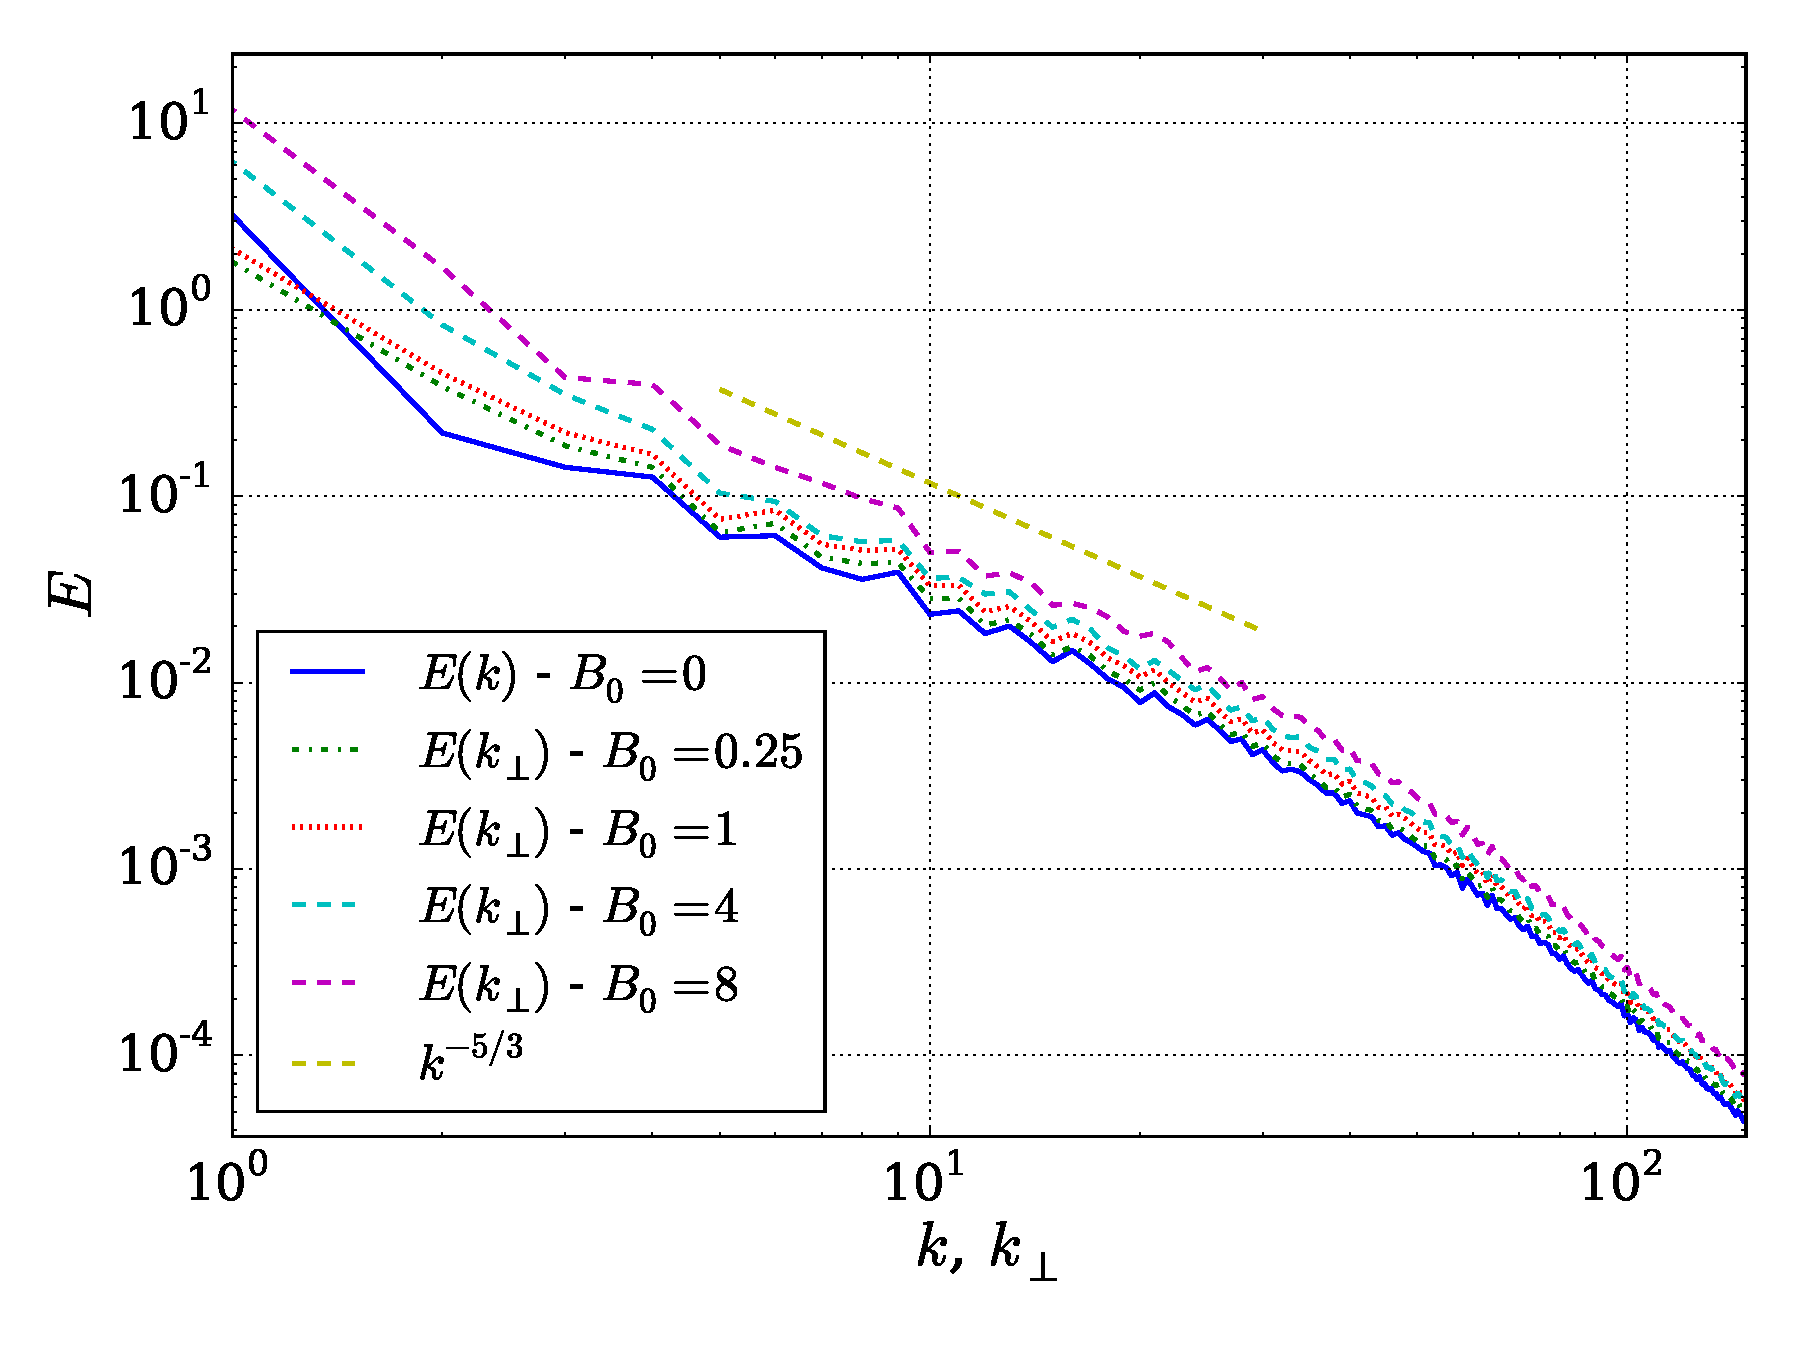
\includegraphics[width=0.8\columnwidth]{SpatioTemporalSpectra/fig1_E-eps-converted-to.pdf}
  \caption{Espectros energéticos perpendiculares reducidos $E(k_\perp)$ para las
  simulaciones con $B_0=0.25$, $1$, $4$, y $8$, y espectro energético
  isotrópico $E(k)$ para la simulación con $B_0=0$. Se muestra como
  referencia el escaleo de Kolmogorov, $\sim k_\perp^{-5/3}$.}
  \label{fig3-1:E}
\end{figure}


La \cref{fig3-2:isocontourns} muestra los contornos de
$e(k_\perp,k_\parallel)/\sin(\theta_k)$, es decir, el espectro
axisimétrico (promediado temporalmente) para las corridas con $B_0=0$,
$B_0=1$, $B_0=4$ y $B_0=8$. Para el flujo isotrópico ($B_0=0$, ver
\cref{fig3-2:isocontourns}a), los contornos de
$e(k_\perp,k_\parallel)/\sin(\theta_k)$ son círculos, tal como se
esperaba [\cite{mininni_isotropization_2012}]. A medida que la
intensidad del campo guía aumenta, la energía se comienza a concentrar
cerca del eje con$k_\parallel=0$, evidenciando la formación de
estructuras elongadas en la dirección del campo guía (o, en otras
palabras, del relativo decrecimiento de los gradientes paralelos del
campo con respecto a los gradientes perpendiculares).

Los tiempos característicos definidos en la
sección \ref{sec3:Wfspectrum_and_Gamma}, $\tau_A$, $\tau_{sw}$ y
$\tau_{nl}$, dividen el espacio de Fourier en
la \cref{fig3-2:isocontourns} en regiones dependiendo de cómo se
ordenan las escalas temporales:
\begin{equation}\label{eq3:Asw} \tau_A < \tau_{sw} \hspace{0.05cm}
\Rightarrow \hspace{0.05cm} k_\perp <
\left(\sqrt{\left(\frac{B_0}{v_{rms}}\right)^2 \cdot
\left(\frac{C_{sw}}{C_A}\right)^2 - 1} \right) k_\parallel,
\end{equation}
\begin{equation}\label{eq3:Anl} \tau_A < \tau_{nl} \hspace{0.05cm}
\Rightarrow \hspace{0.05cm} k_\perp <
\left(\sqrt{\left(\frac{B_0}{v_{rms}}\right)^3
\left(\frac{C_{nl}}{C_A}\right)^3 Lk_\parallel - 1} \right) 
k_\parallel,
\end{equation}
\begin{equation}\label{eq3:nlsw} \tau_{nl} < \tau_{sw} \hspace{0.05cm}
\Rightarrow \hspace{0.05cm} \left( k_\perp^2 + k_\parallel^2
\right)^{1/6} < \frac{C_{sw}}{C_{nl}L^{1/3}}.
\end{equation}
En la \cref{fig3-2:isocontourns} también se indican las curvas
correspondientes a los modos que satisfacen las relaciones
$\tau_A\lesssim\tau_{sw}$ y $\tau_A\lesssim\tau_{nl}$, para $B_0=1$,
$4$ y $8$ (asumiendo, para dibujar las curvas, que $C_{sw} \approx
C_{nl} \approx C_A \approx 1$; esta elección fue posteriormente
confirmada por el análisis de las funciones de correlación). Debe
mencionarse que la curva $\tau_A\approx\tau_{nl}$ también cumple un
rol muy importante en la teoría de balances críticos
[\cite{sridhar_toward_1994}].

Como puede verse de la \cref{eq3:nlsw}, la región donde
$\tau_{nl}\leq\tau_{sw}$ es un círculo pequeño alrededor del origen,
donde $k_\perp^2 + k_\parallel^2 \leq (C_{sw}/L^{1/3}C_{nl})^6 \approx
1$, y no se puede ver en la figura. Los modos fuera de la región con
$\tau_{nl}<\tau_{sw}$ deberían descorrelacionarse con el tiempo de
\textit{sweeping} o con el tiempo de Alfvén, dependiendo de cuál sea
más rápido. La \cref{eq3:Asw} nos dice que en el área a la izquierda de
la curva $\tau_A\sim\tau_{sw}$ tenemos $\tau_A<\tau_{sw}$, mientras
que la \cref{eq3:Anl} nos dice que en el área a la izquierda de la
curva $\tau_A\sim\tau_{nl}$ tenemos $\tau_A<\tau_{nl}$ (ver
\cref{fig3-2:isocontourns}b). Para el valor más grande de $B_0$
considerado (i.e., la simulación con $B_0=8$), la mayoría de los modos
tienen al periodo de Alfvén como el tiempo más rápido (i.e., la mayor
área en el gráfico se encuentre arriba y a la izquierda de la curva
$\tau_A \sim \tau_{sw}$), a pesar de que una fracción significativa de
la energía en el sistema no esté en estos modos, sino que se
concentran cerca del eje con $k_\parallel = 0$.

\begin{figure*}
  \centering
%  \subfigure[$B_0=0$]{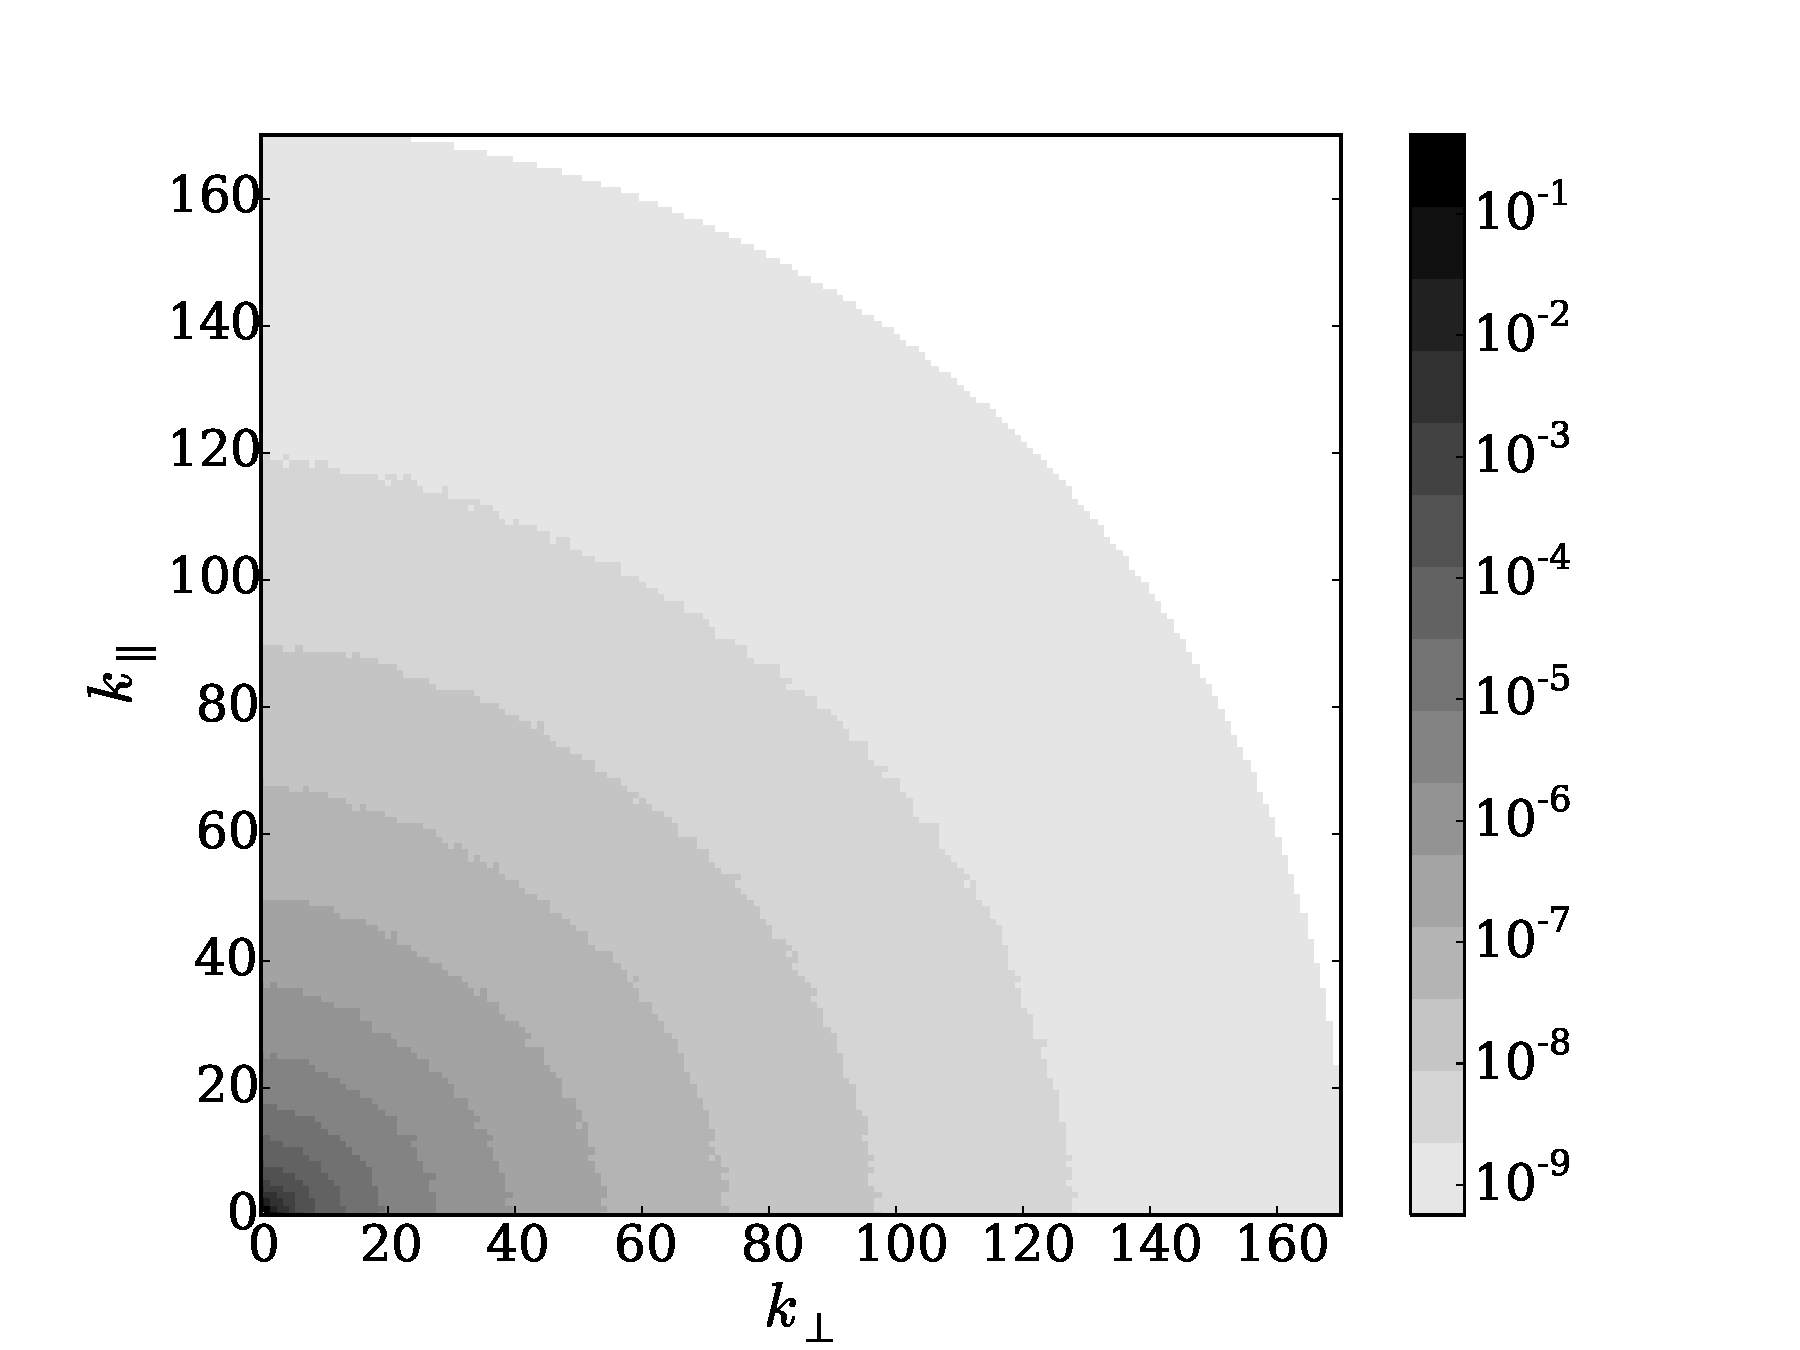
\includegraphics[width=0.45\textwidth]{SpatioTemporalSpectra/fig2_B0-eps-converted-to.pdf}}
%  \subfigure[$B_0=0.25$]{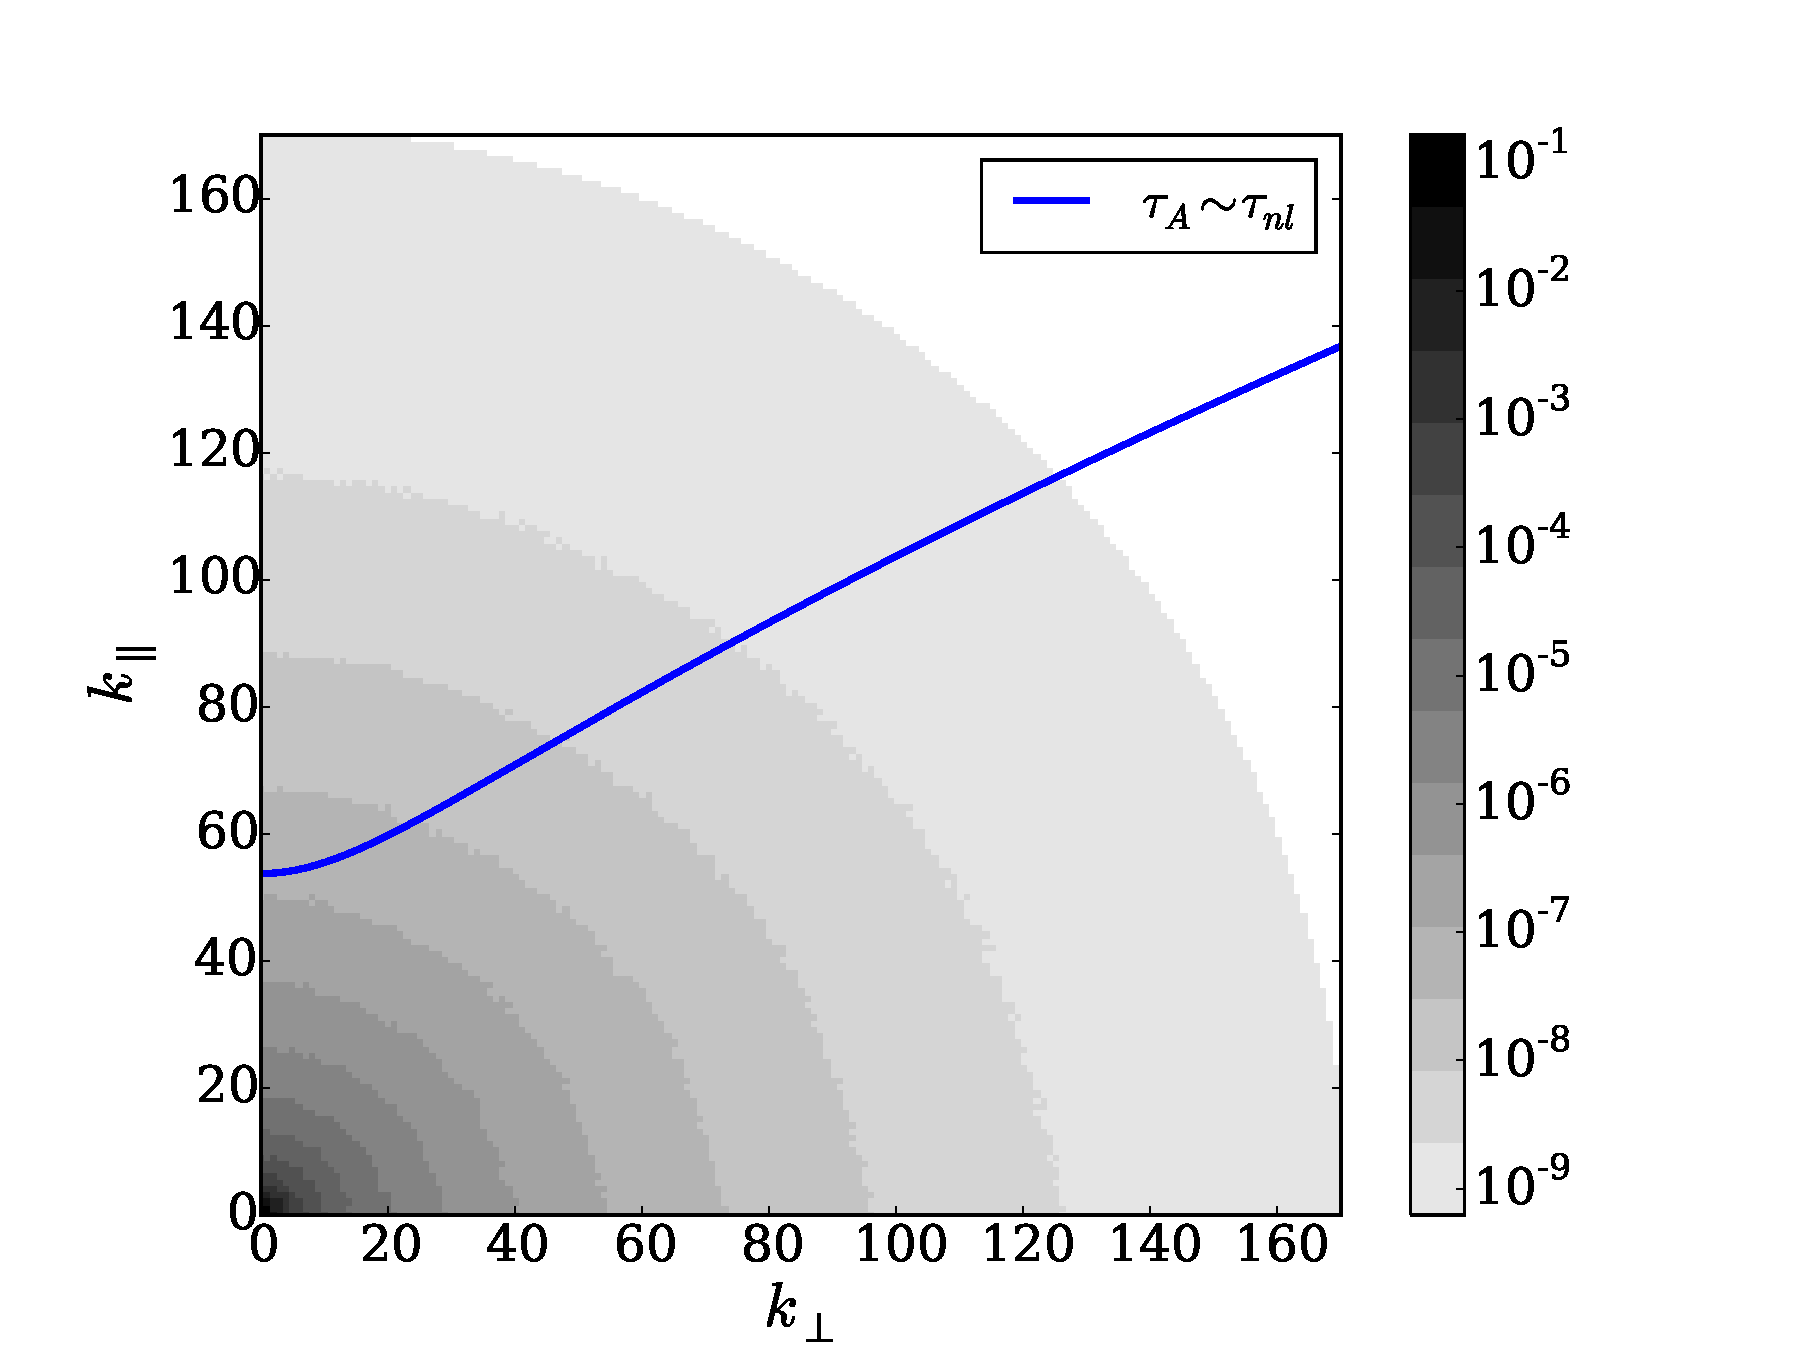
\includegraphics[width=0.45\textwidth]{SpatioTemporalSpectra/fig2_B025-eps-converted-to.pdf}}

%  \subfigure[$B_0=1$]{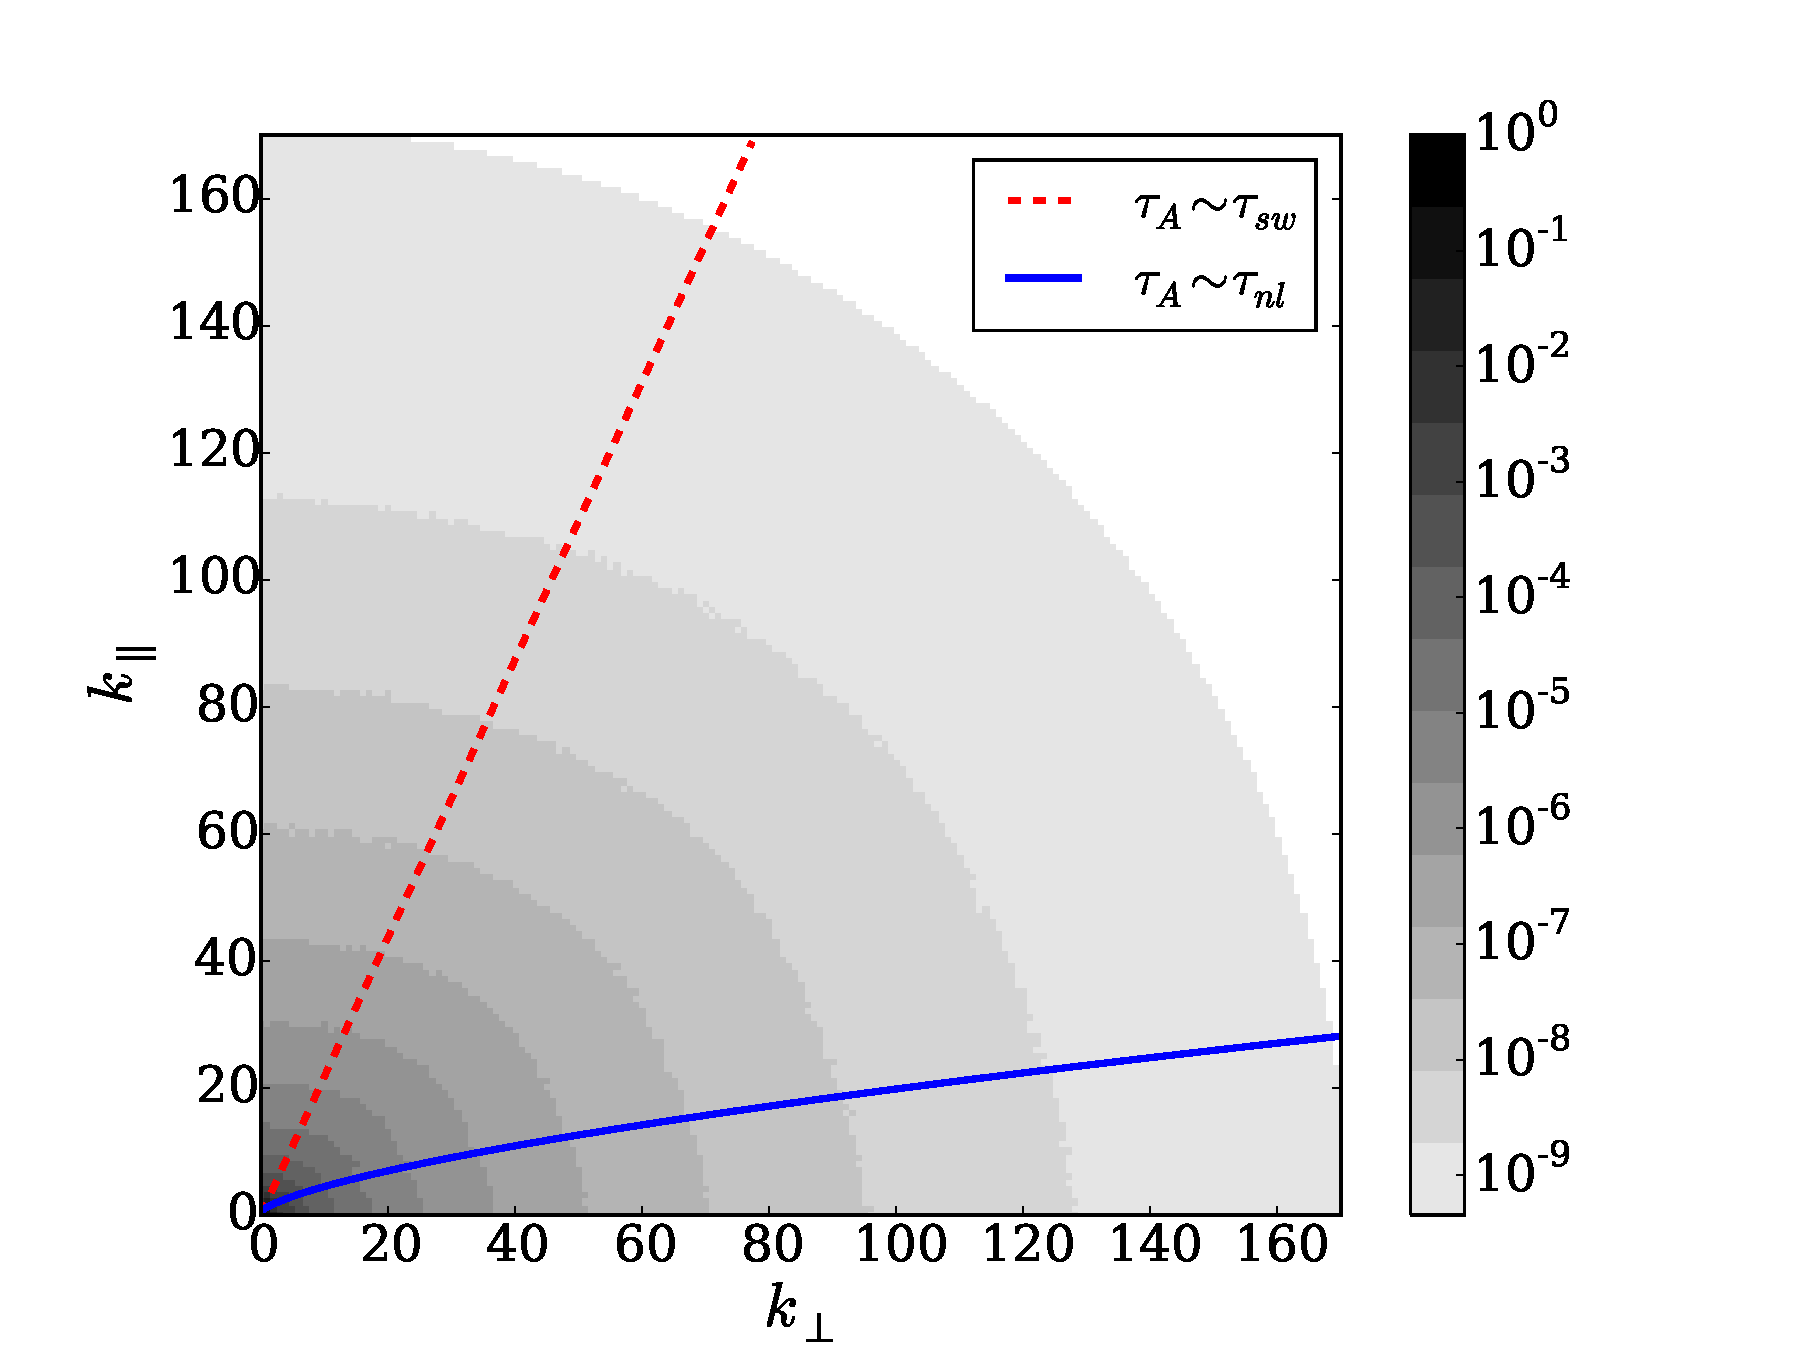
\includegraphics[width=0.45\textwidth]{SpatioTemporalSpectra/fig2_B1-eps-converted-to.pdf}}
%  \subfigure[$B_0=1$ with explanation]{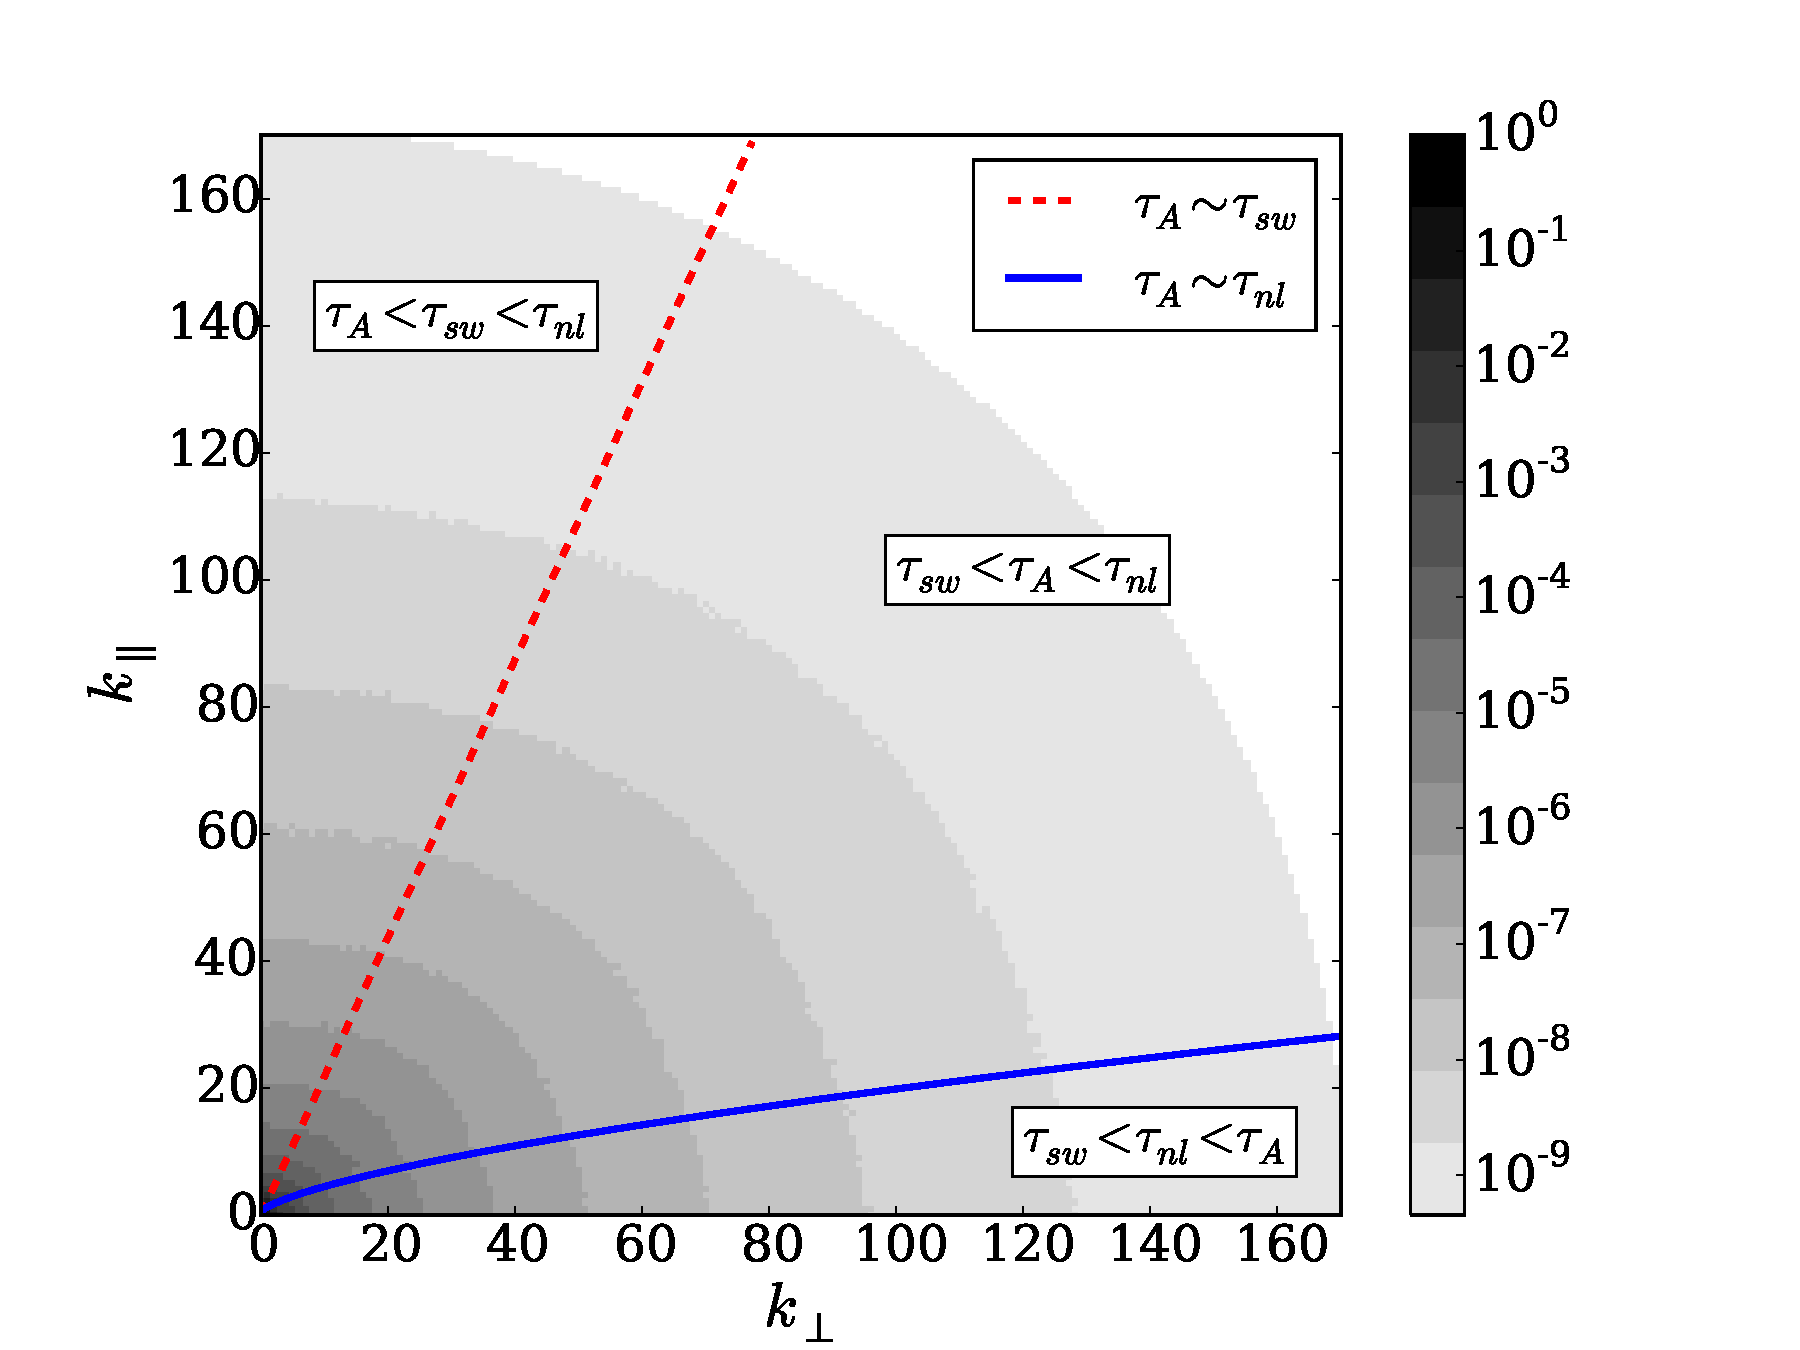
\includegraphics[width=0.45\textwidth]{SpatioTemporalSpectra/fig2_B1_explanation-eps-converted-to.pdf}}

%  \subfigure[$B_0=4$]{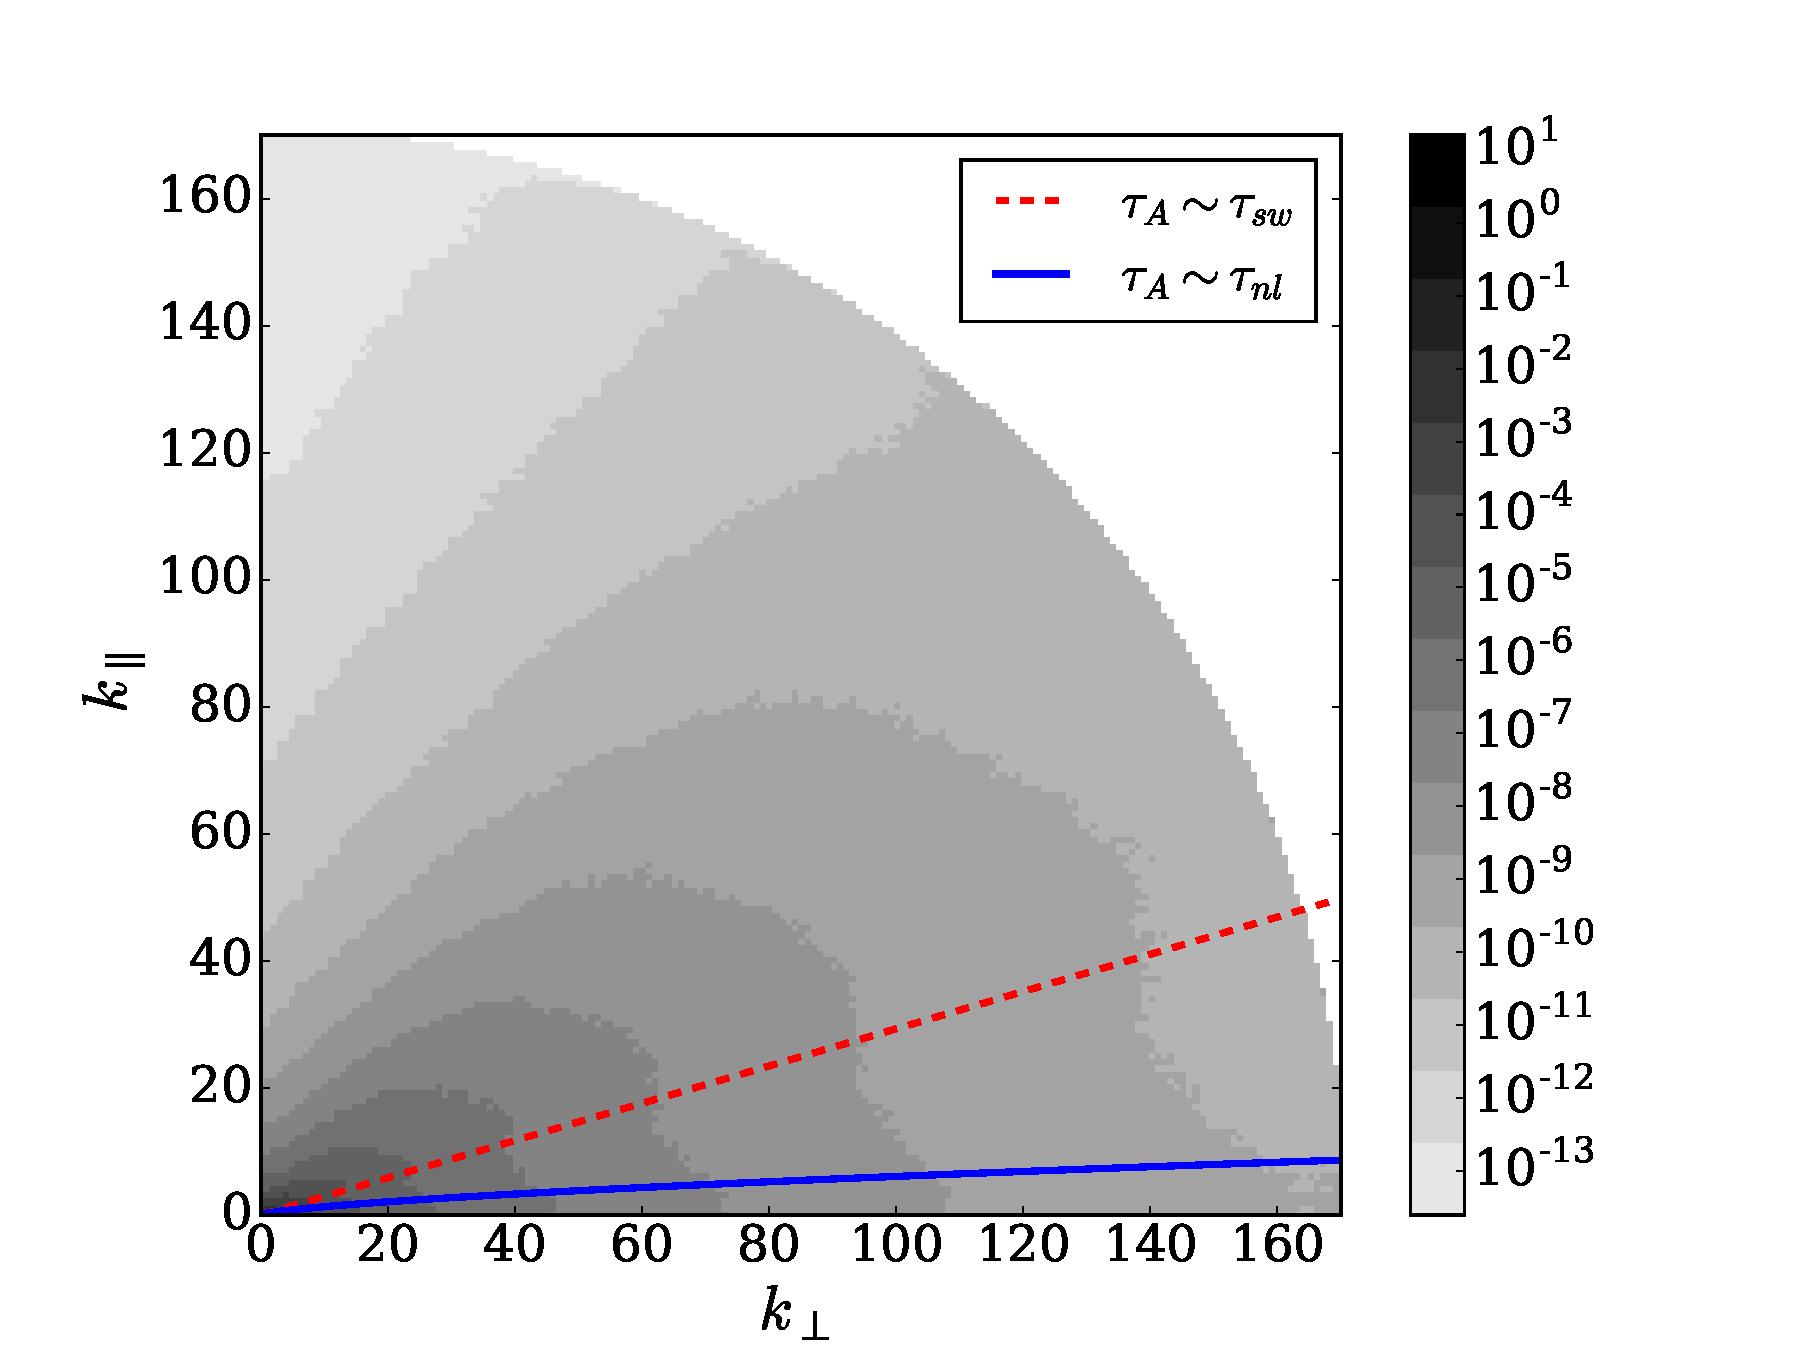
\includegraphics[width=0.45\textwidth]{SpatioTemporalSpectra/fig2_B4-eps-converted-to.pdf}}
%  \subfigure[$B_0=8$]{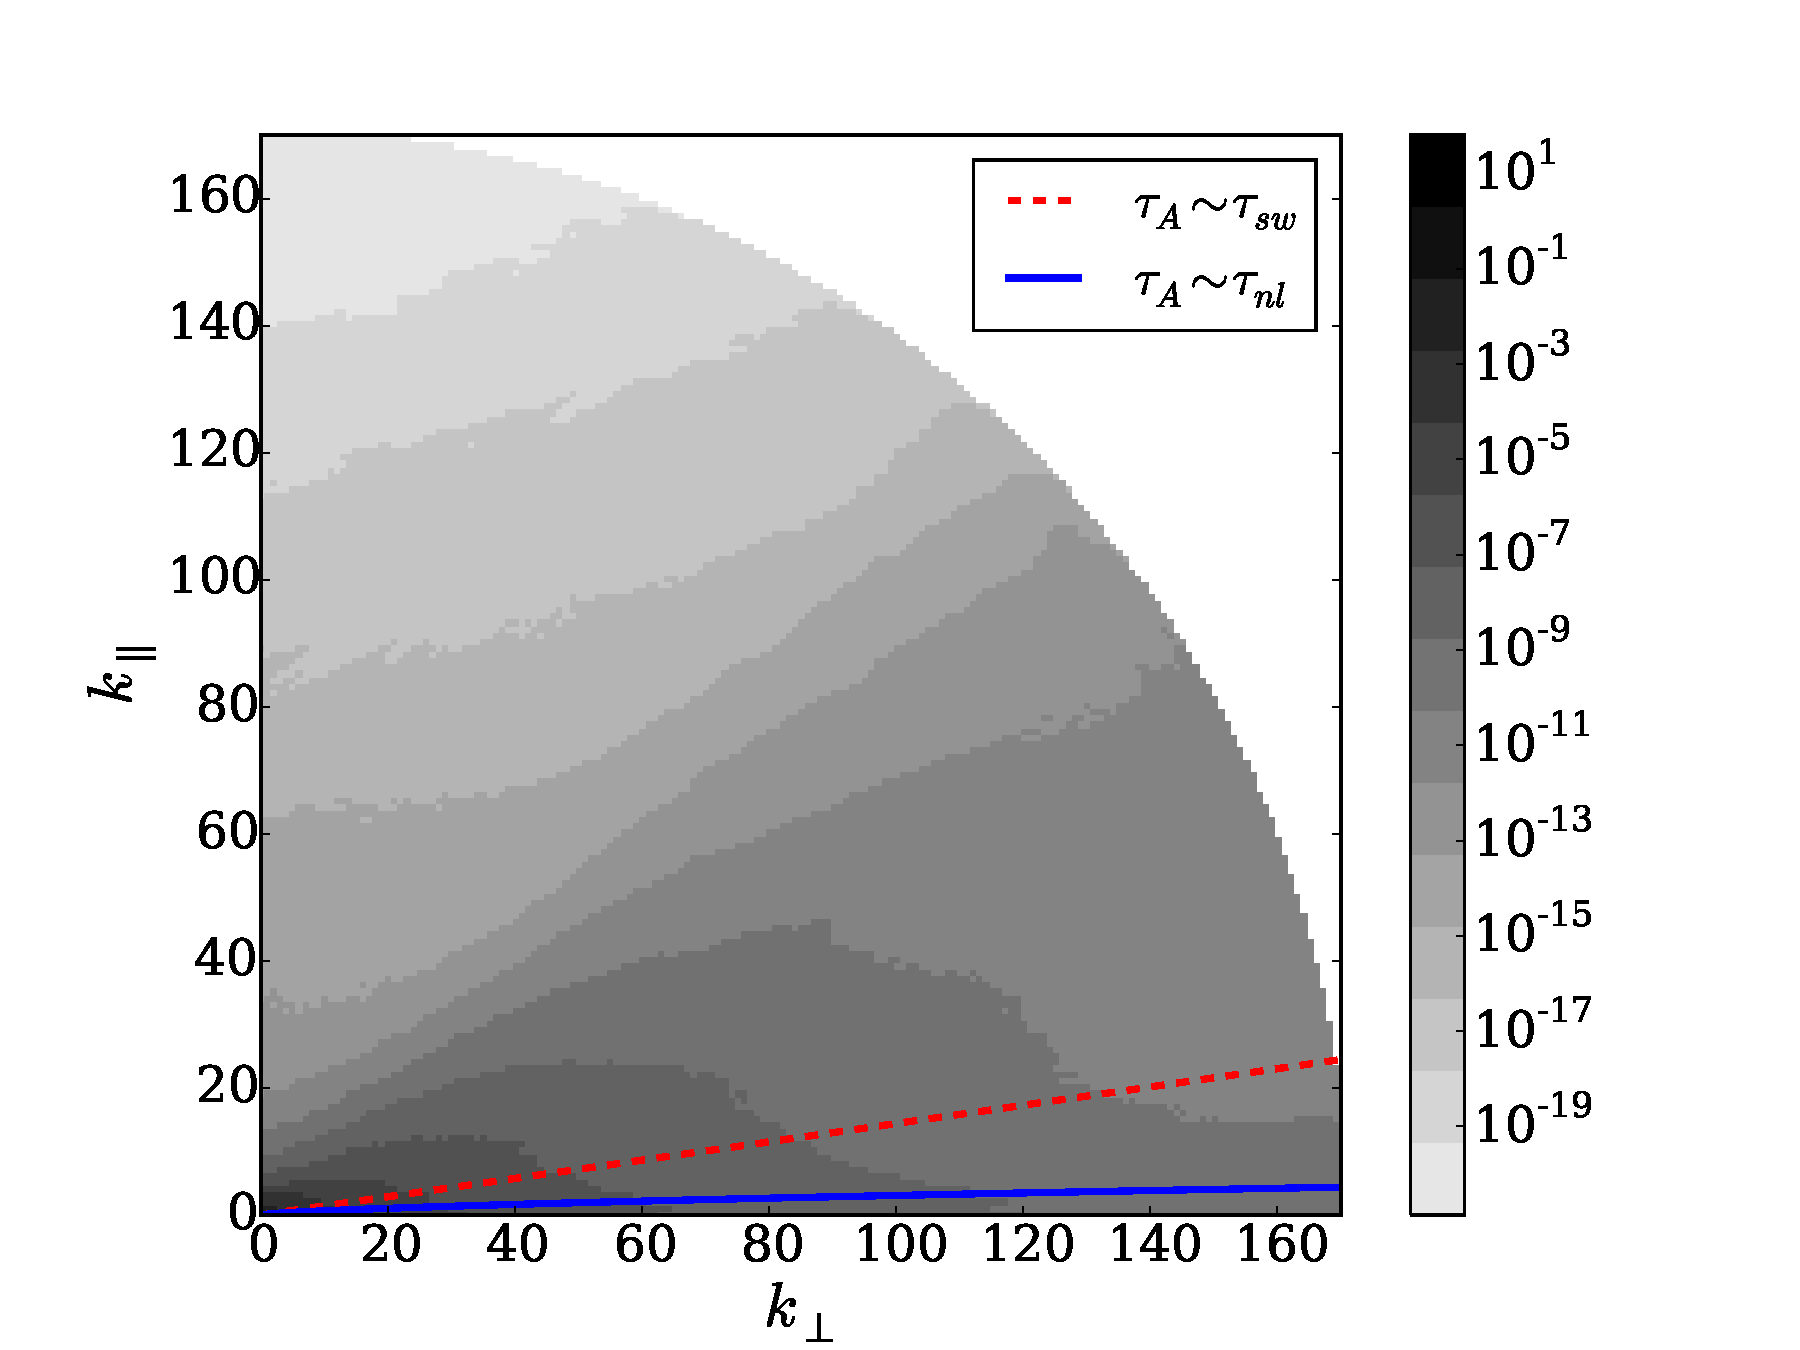
\includegraphics[width=0.45\textwidth]{SpatioTemporalSpectra/fig2_B8-eps-converted-to.pdf}}
  \subfigure[$B_0=0$]{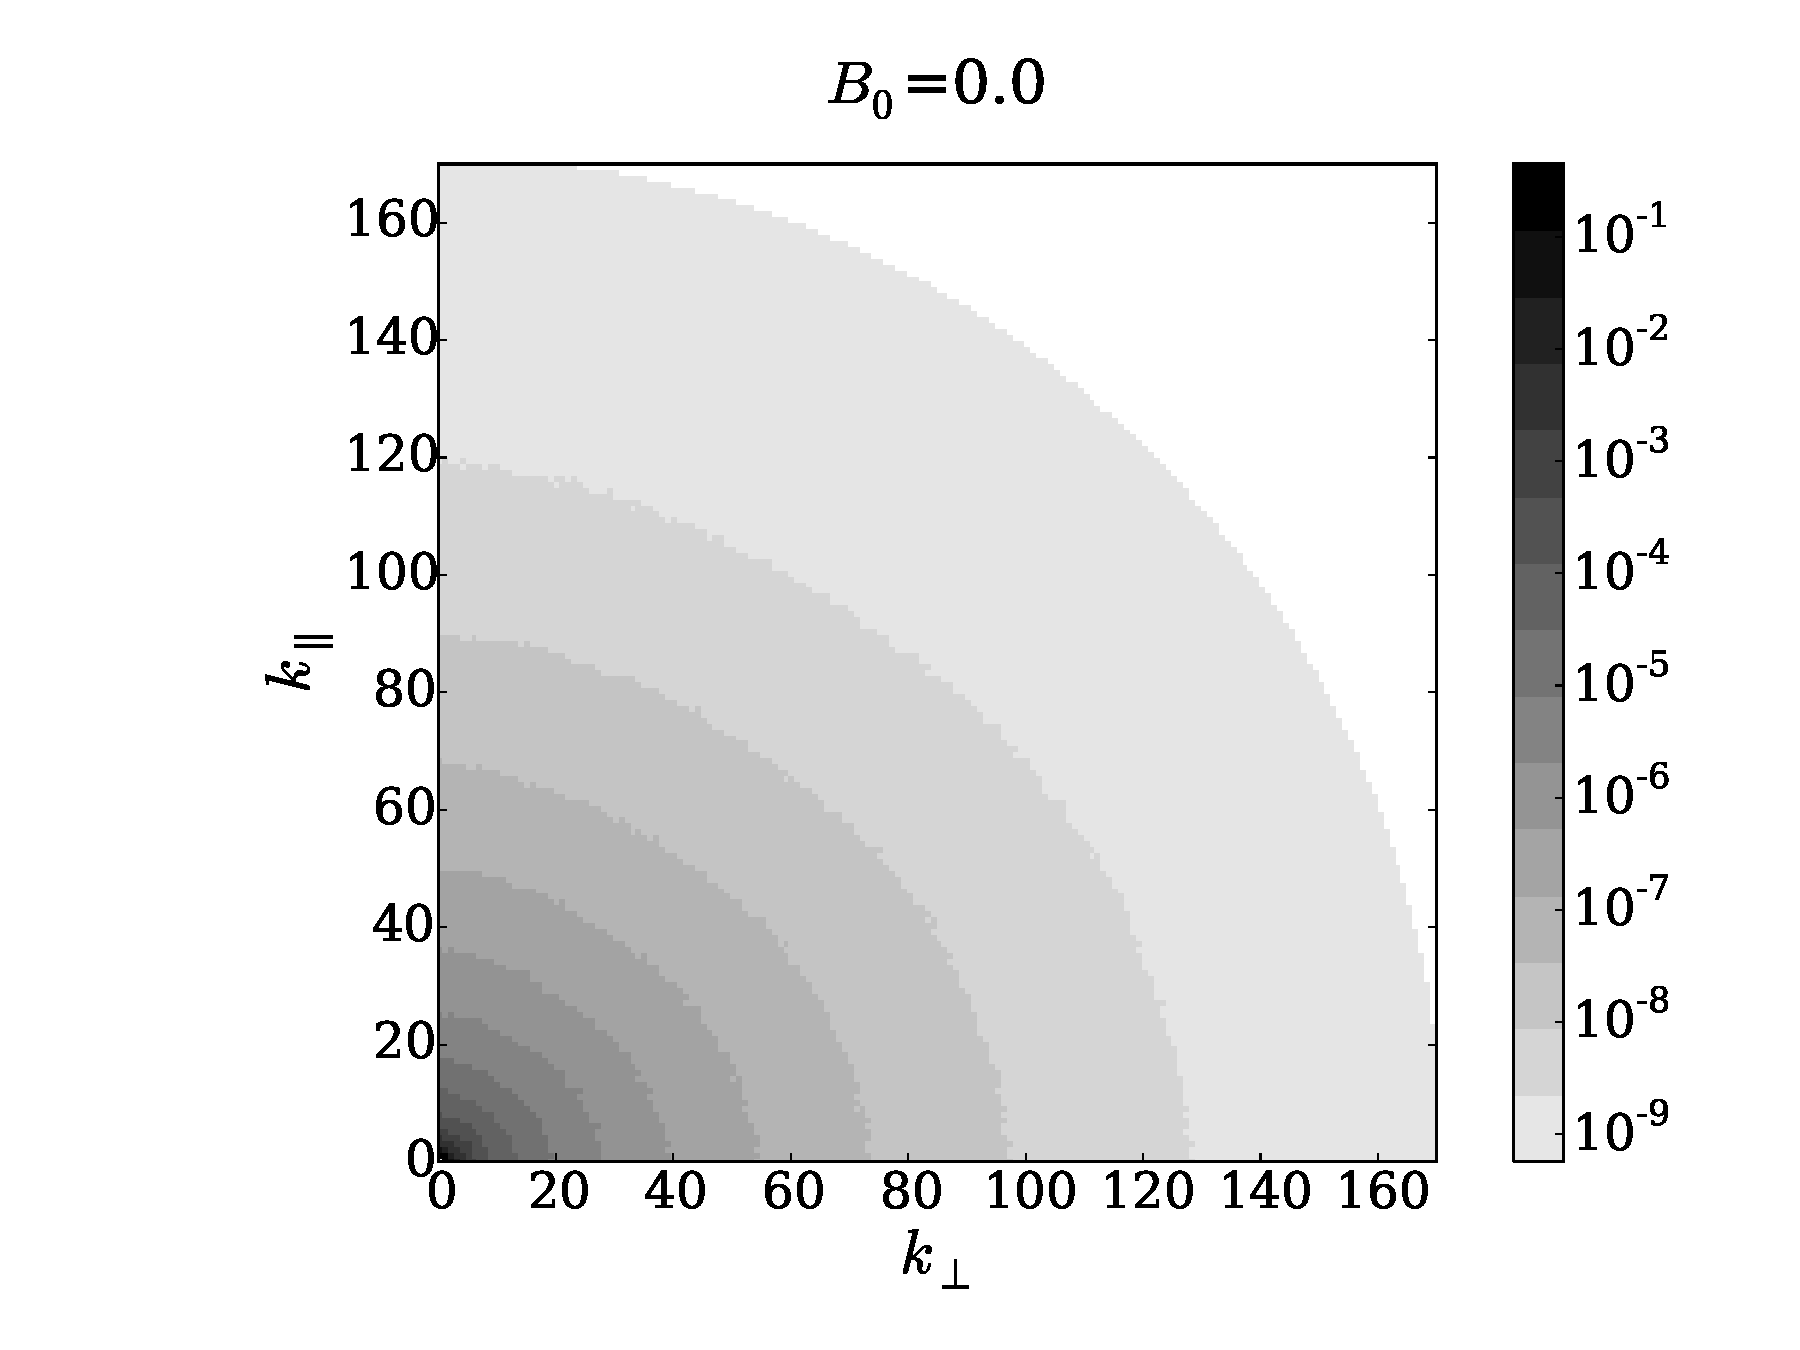
\includegraphics[width=0.48\textwidth]{SpatioTemporalSpectra/fig2_B0.pdf}}\hfill
  \subfigure[$B_0=1$]{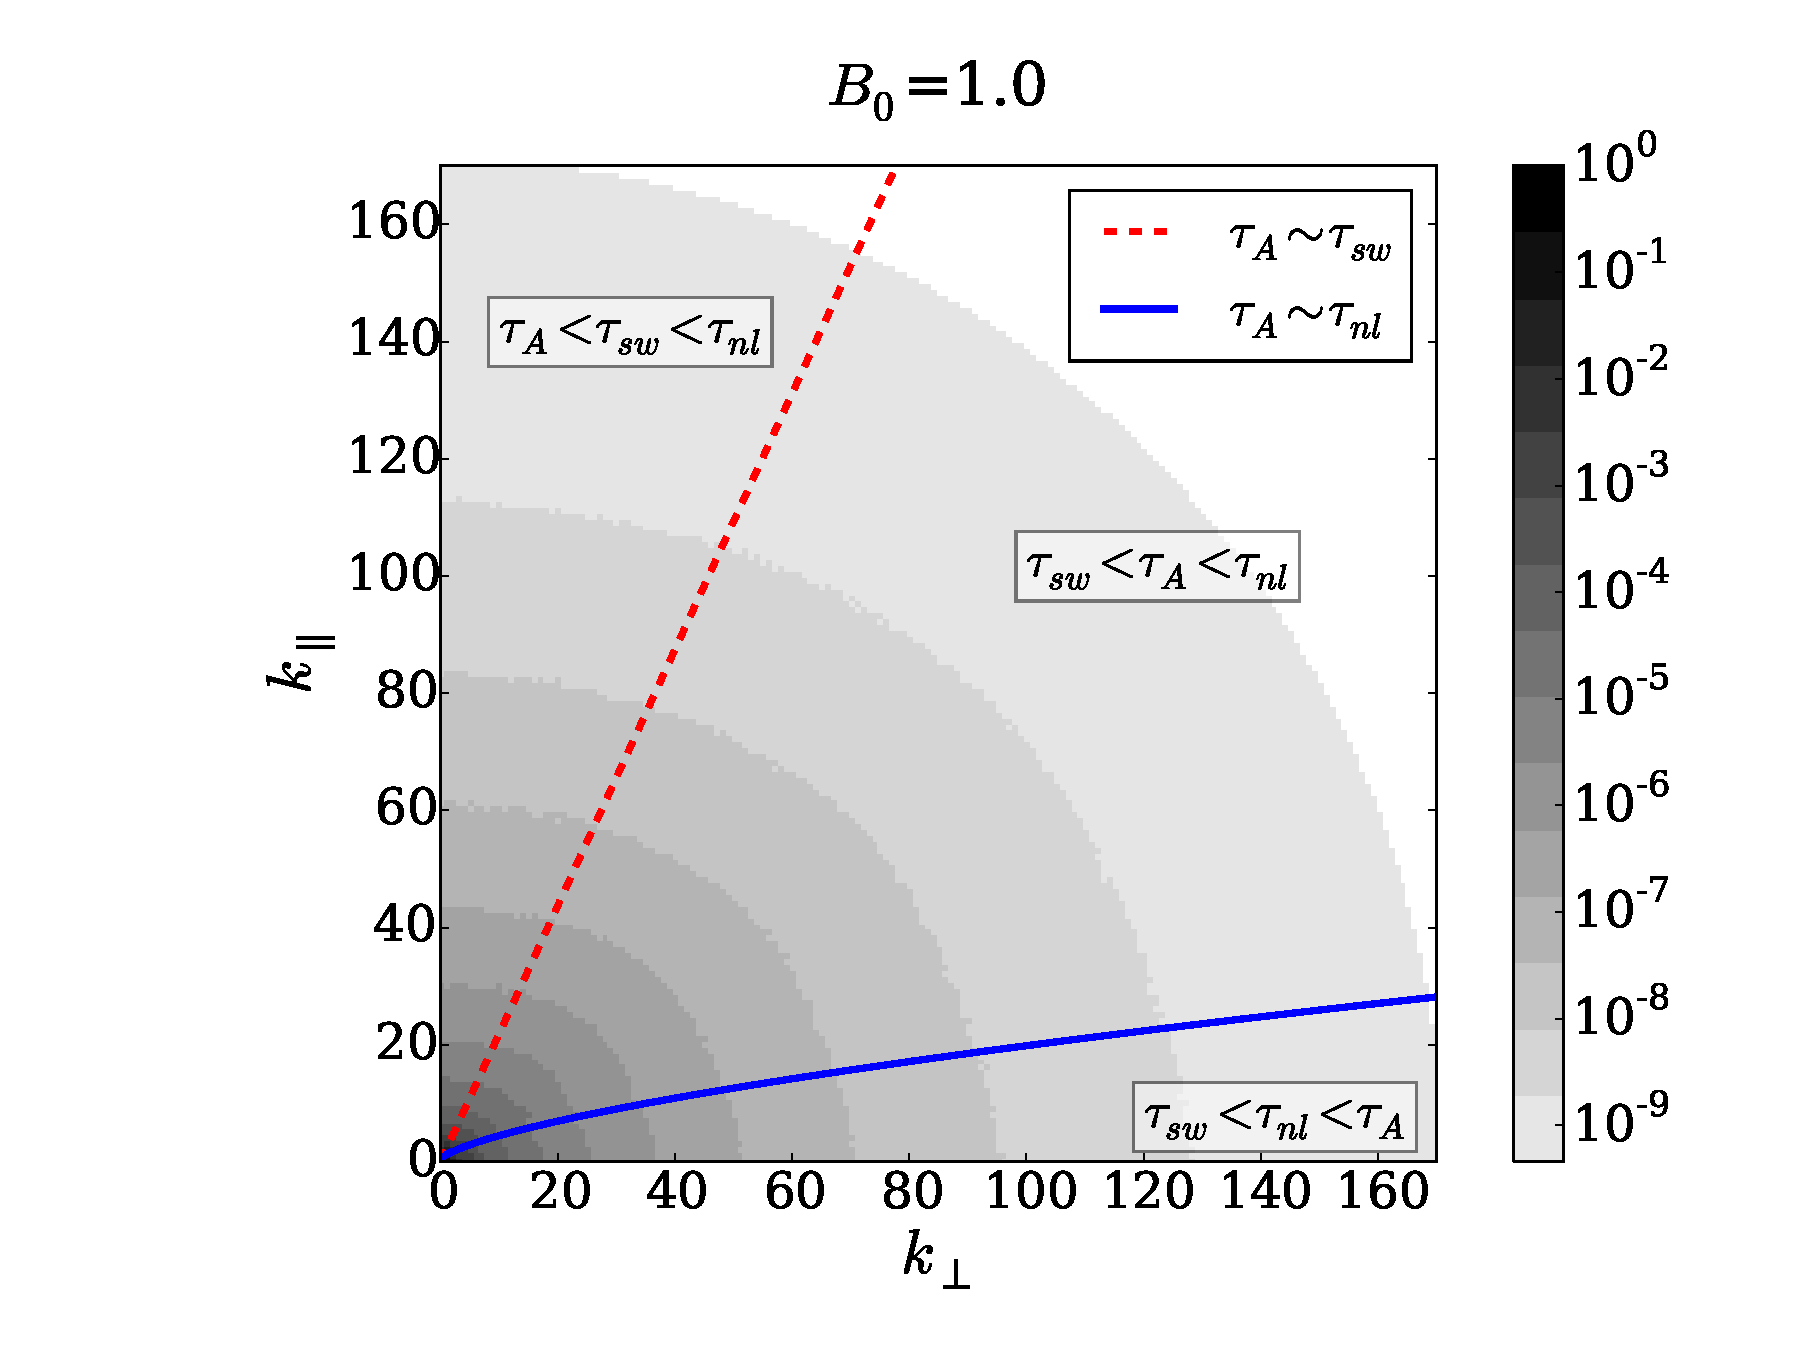
\includegraphics[width=0.48\textwidth]{SpatioTemporalSpectra/fig2_B1.pdf}}

  \subfigure[$B_0=4$]{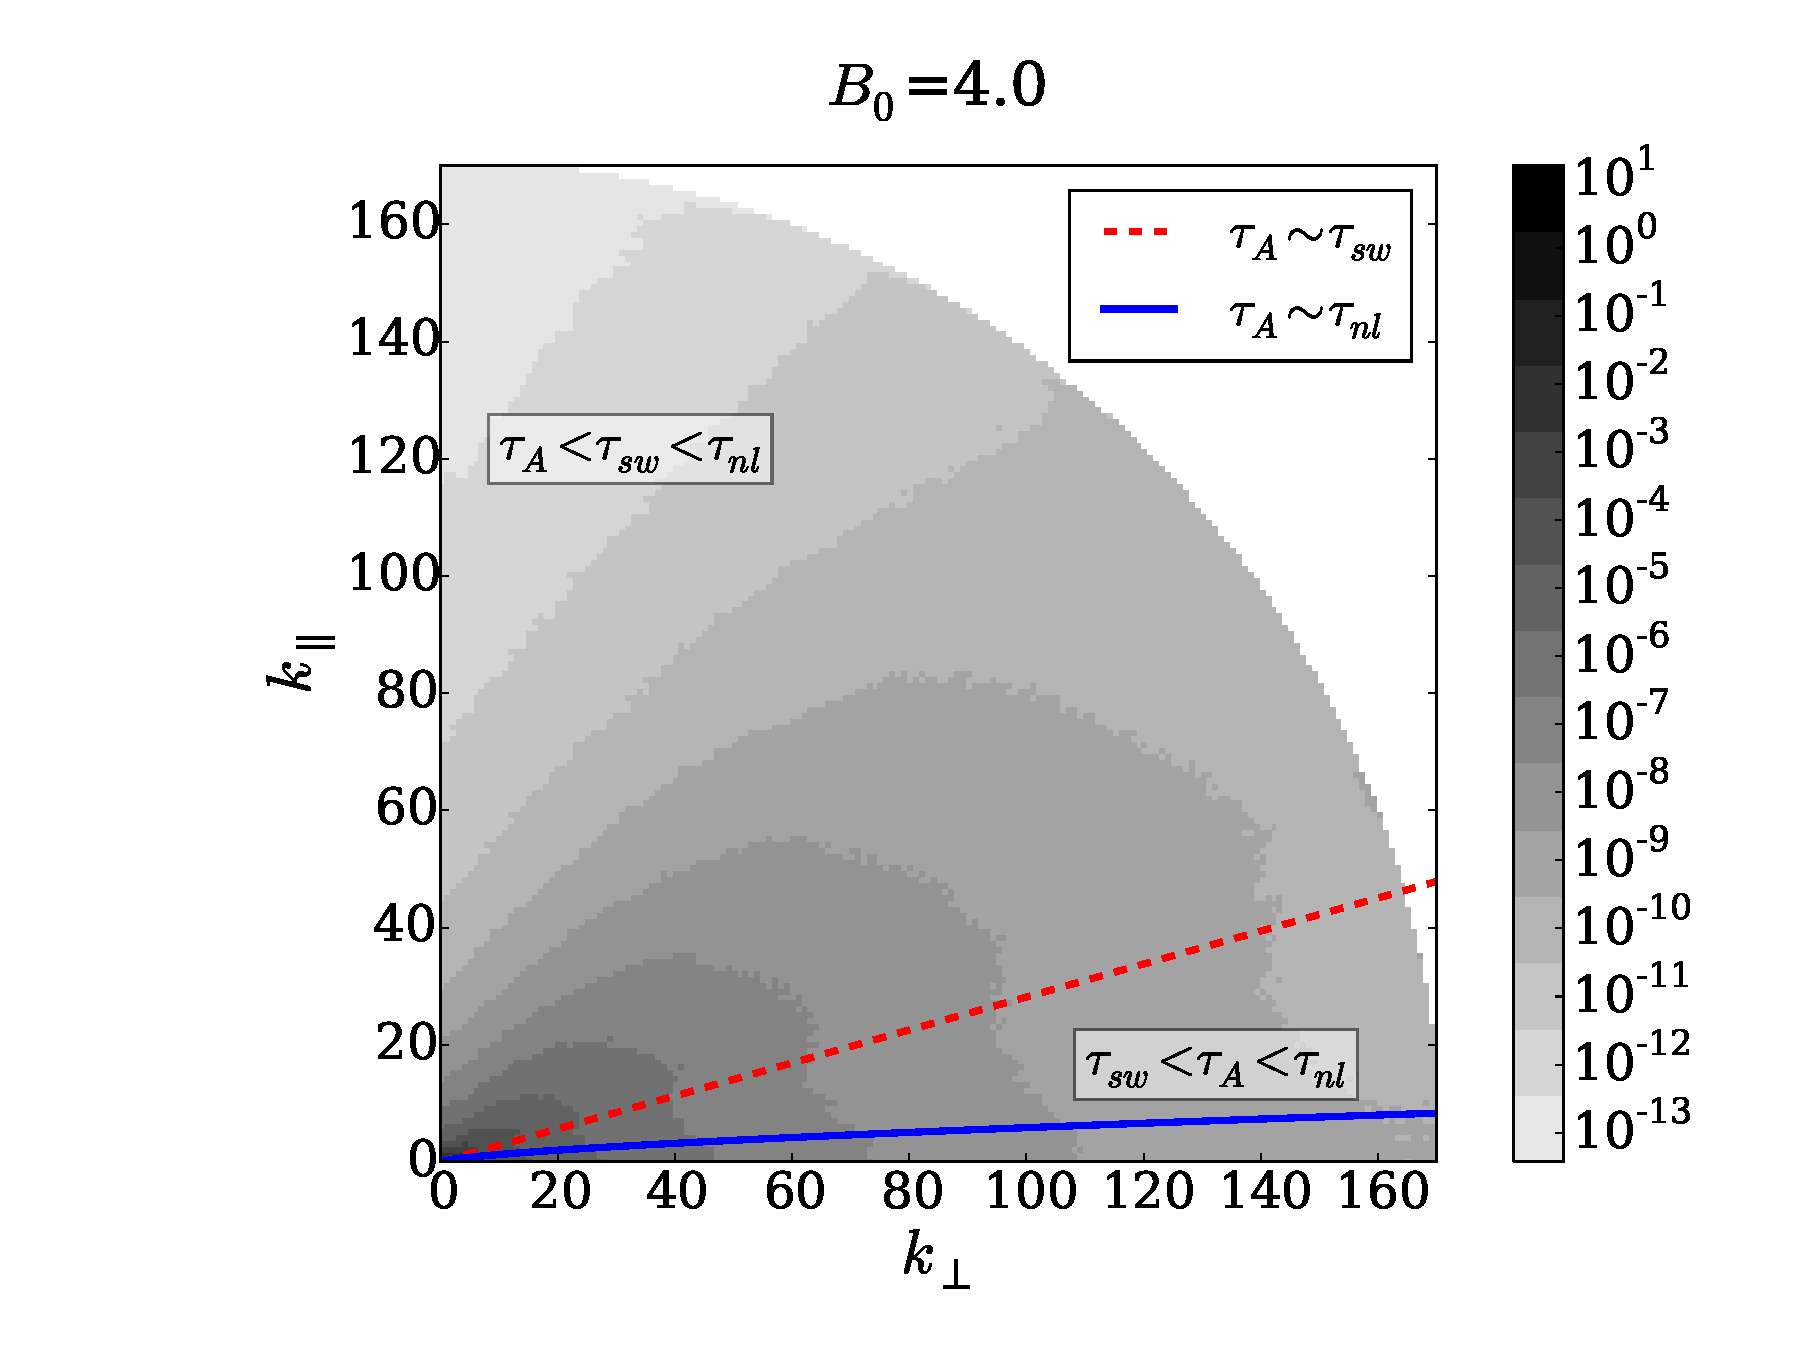
\includegraphics[width=0.48\textwidth]{SpatioTemporalSpectra/fig2_B4.pdf}}\hfill
  \subfigure[$B_0=4$ en escala doble logaritmo]{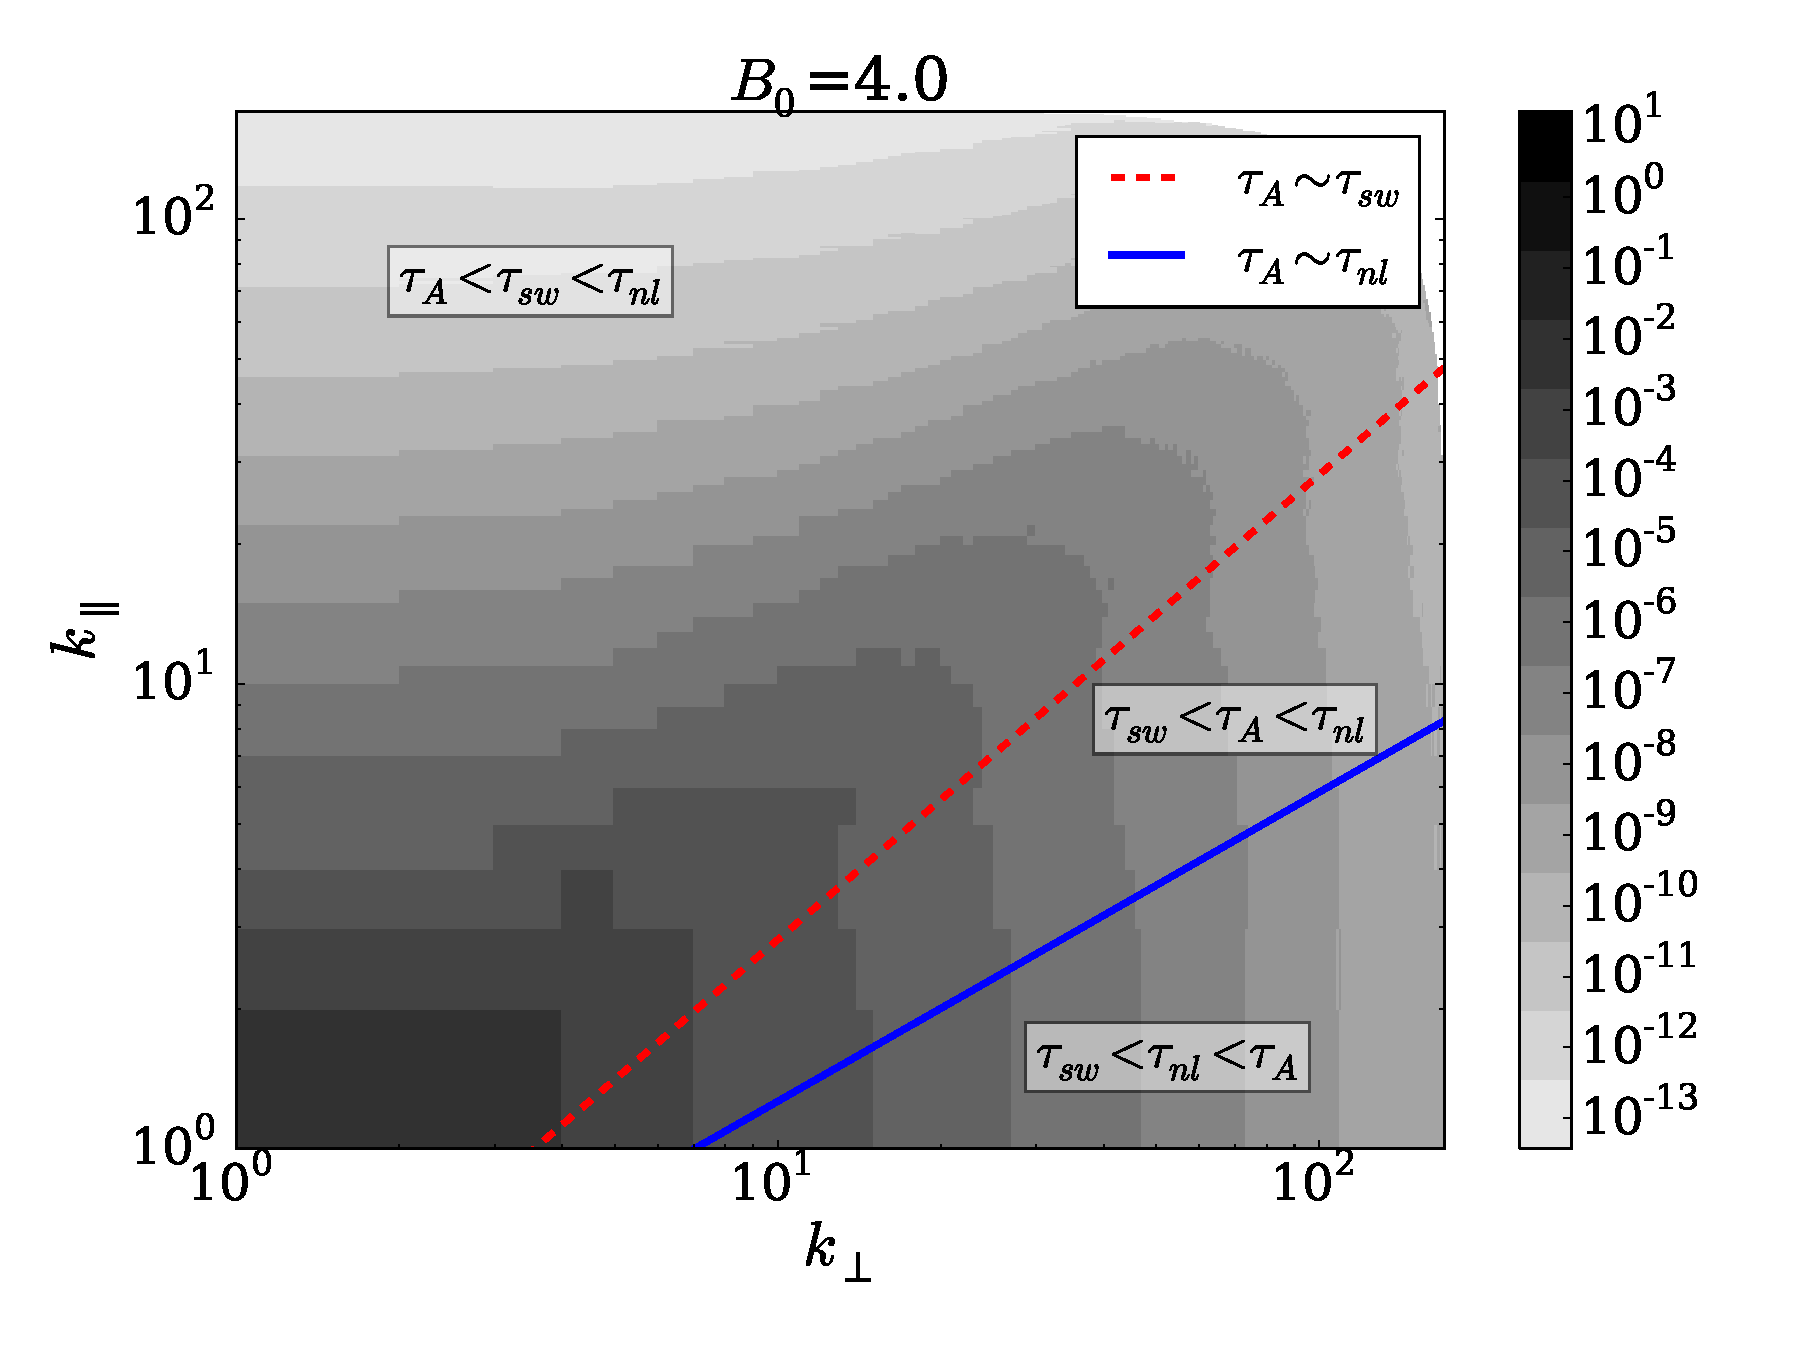
\includegraphics[width=0.48\textwidth]{SpatioTemporalSpectra/fig2_B4_log.pdf}}
%  \subfigure[$B_0=4$ in log-log scale]{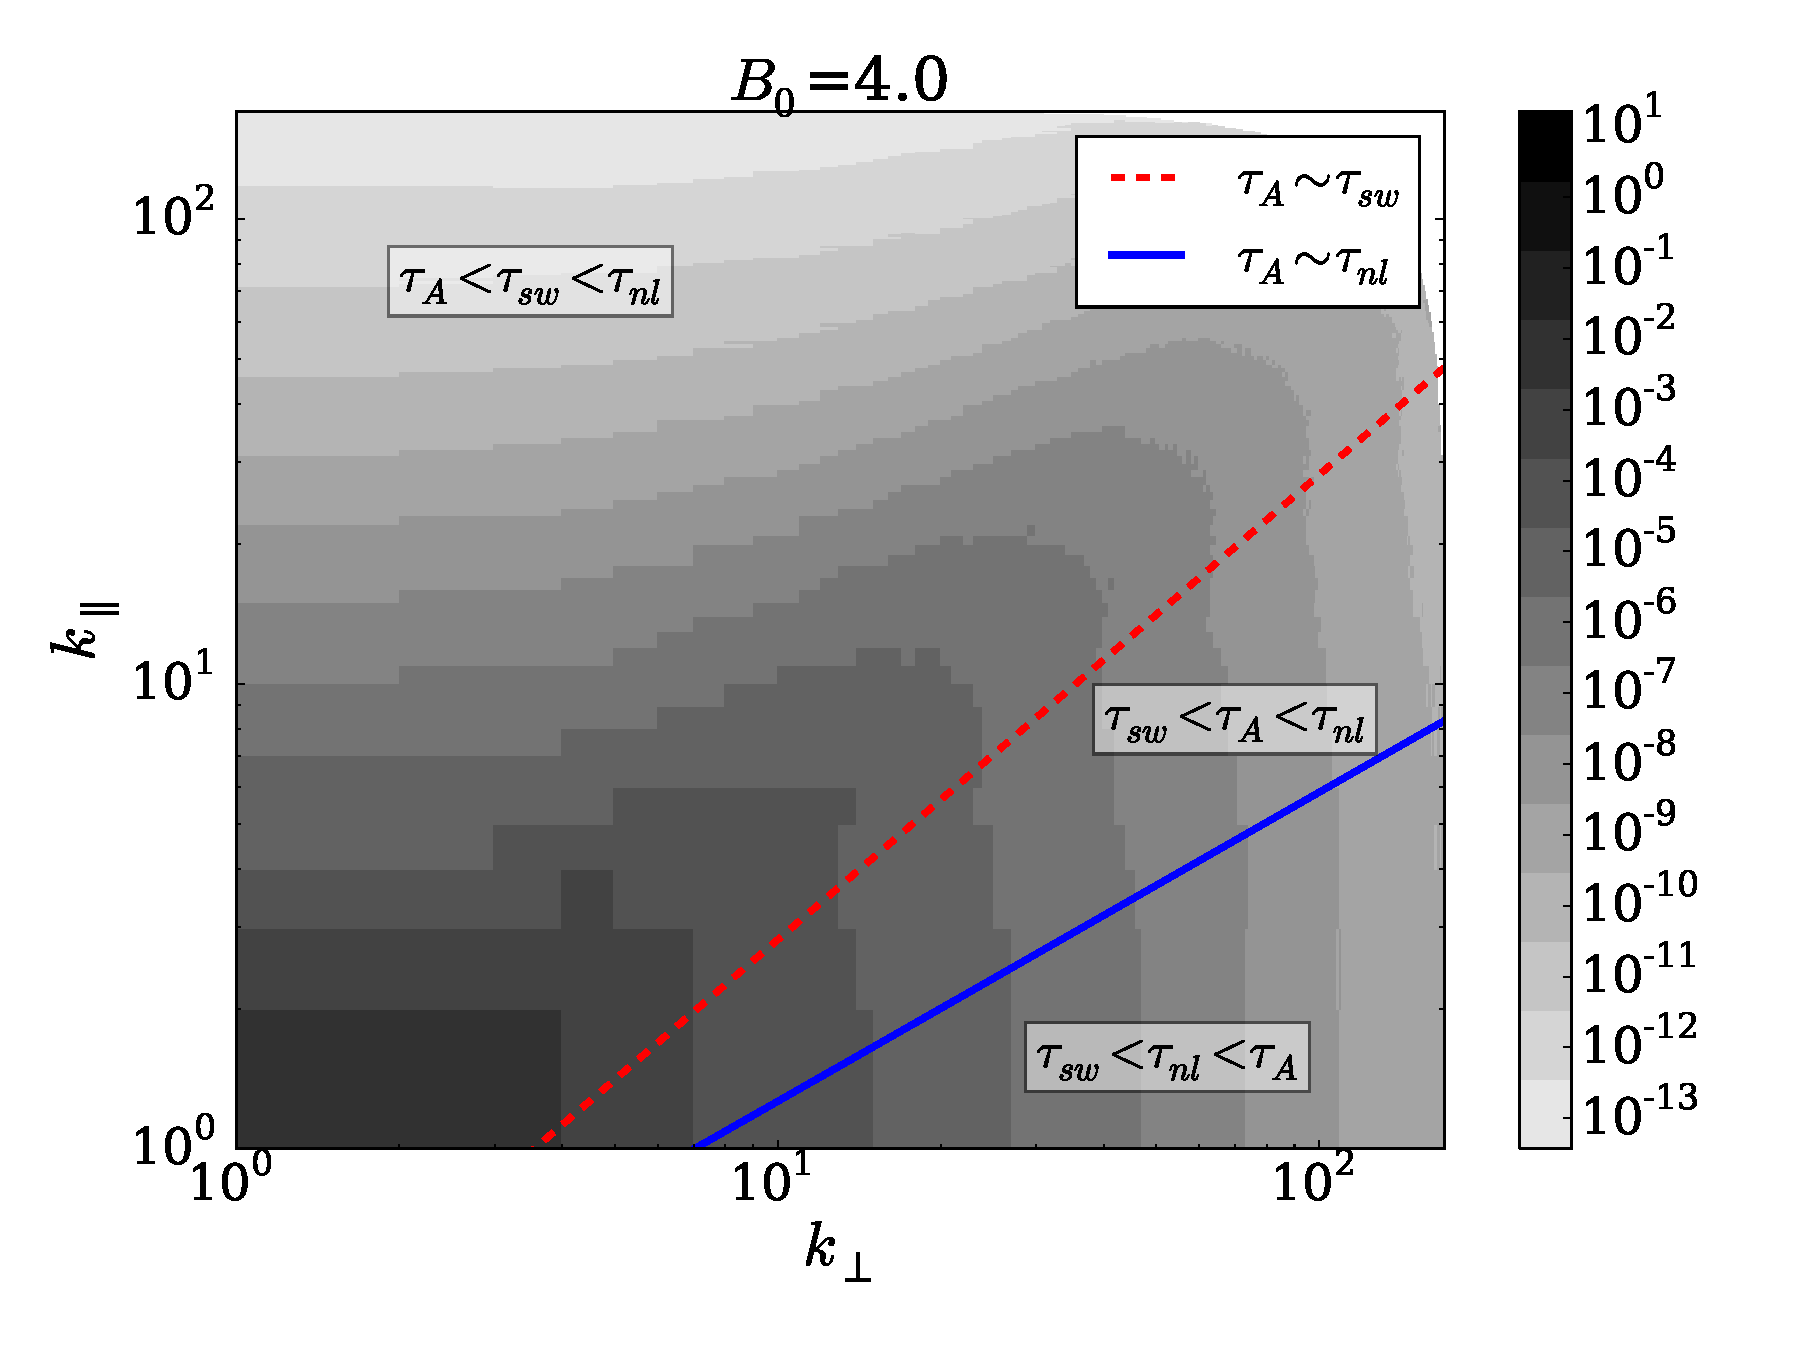
\includegraphics[width=0.45\textwidth]{SpatioTemporalSpectra/fig2_B4_log.eps}}

  \subfigure[$B_0=8$]{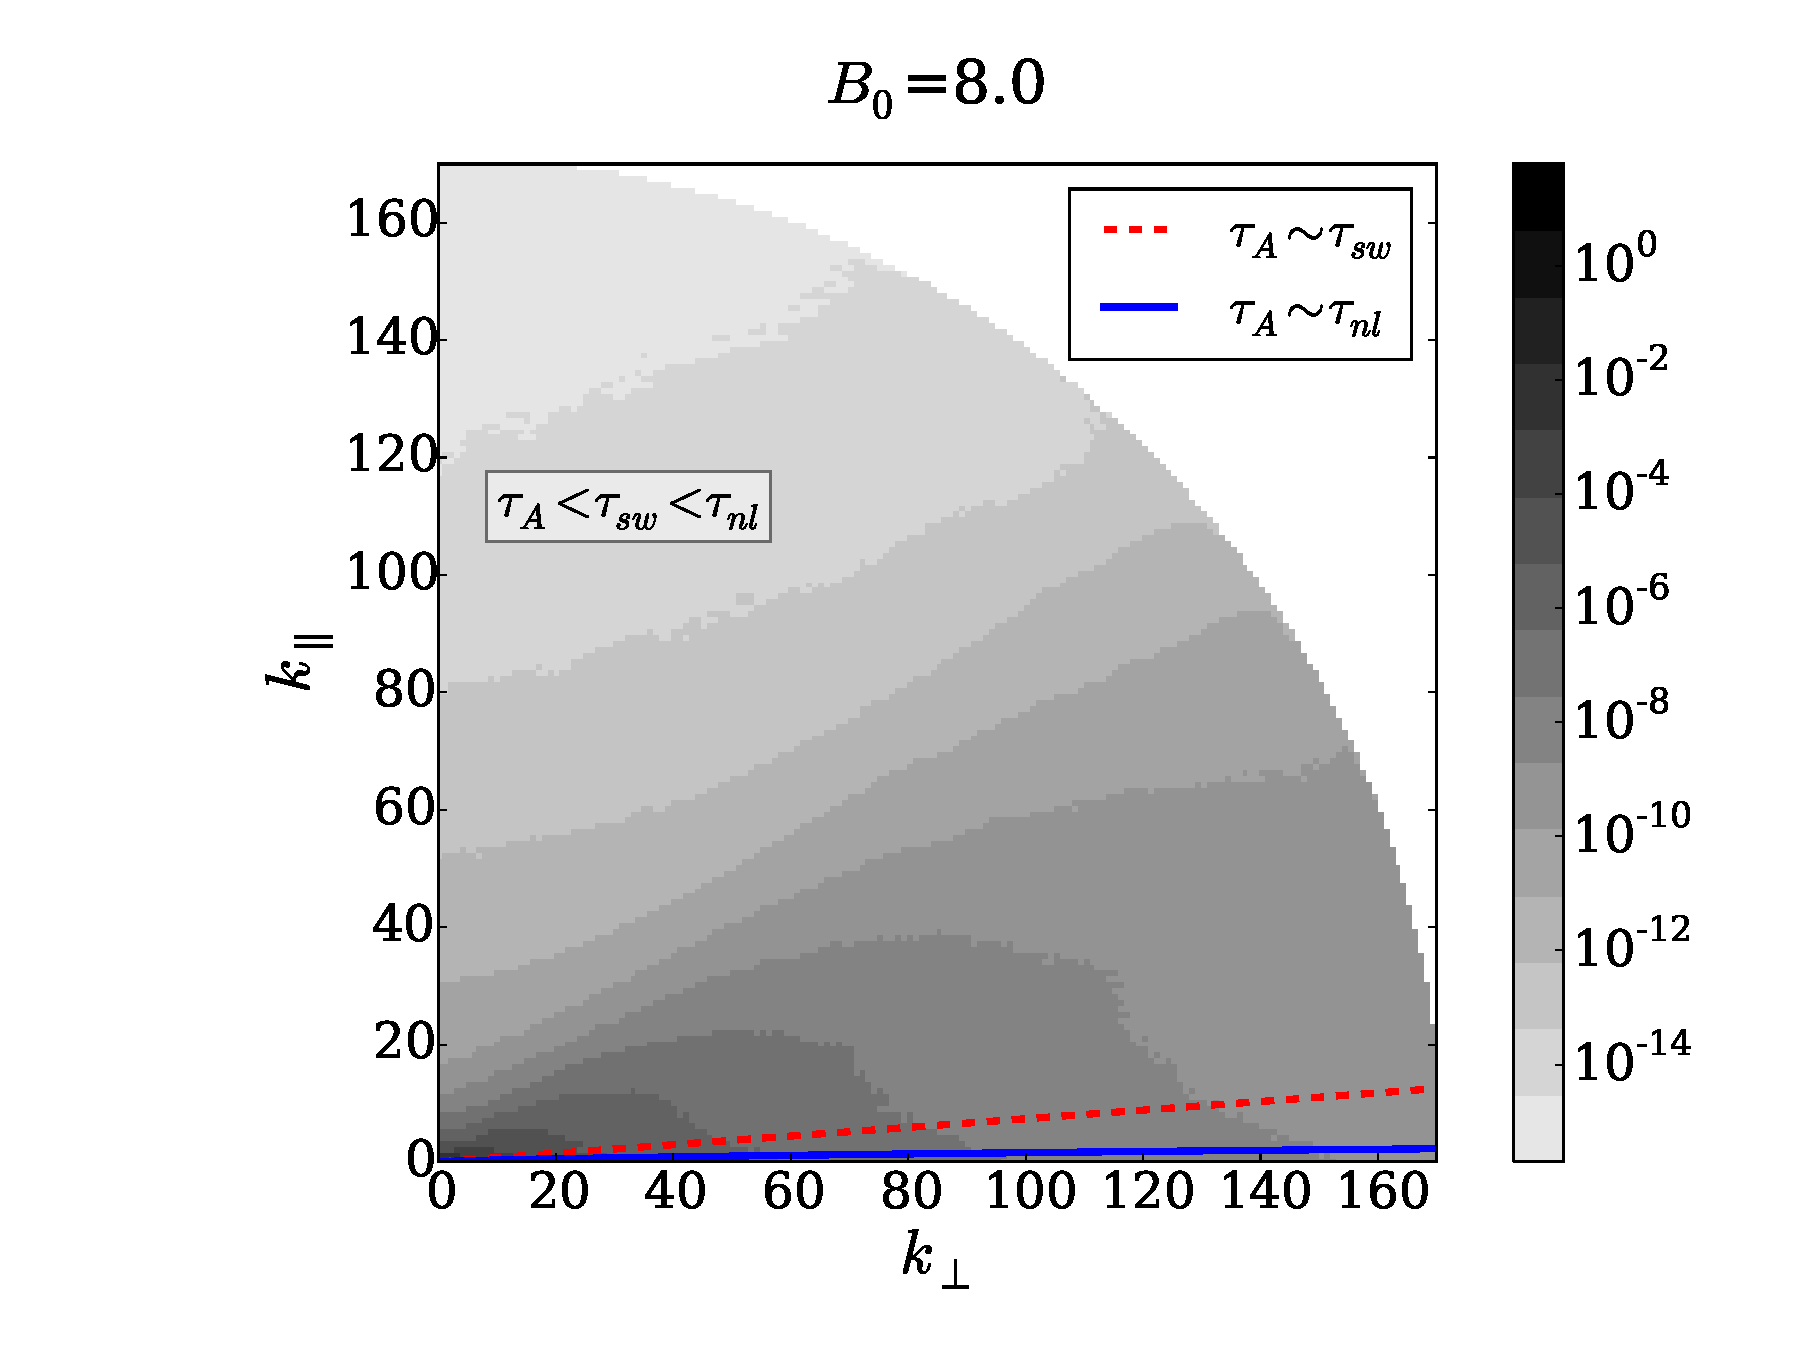
\includegraphics[width=0.48\textwidth]{SpatioTemporalSpectra/fig2_B8.pdf}}\hfill
  \subfigure[$B_0=8$ en escala doble logaritmo]{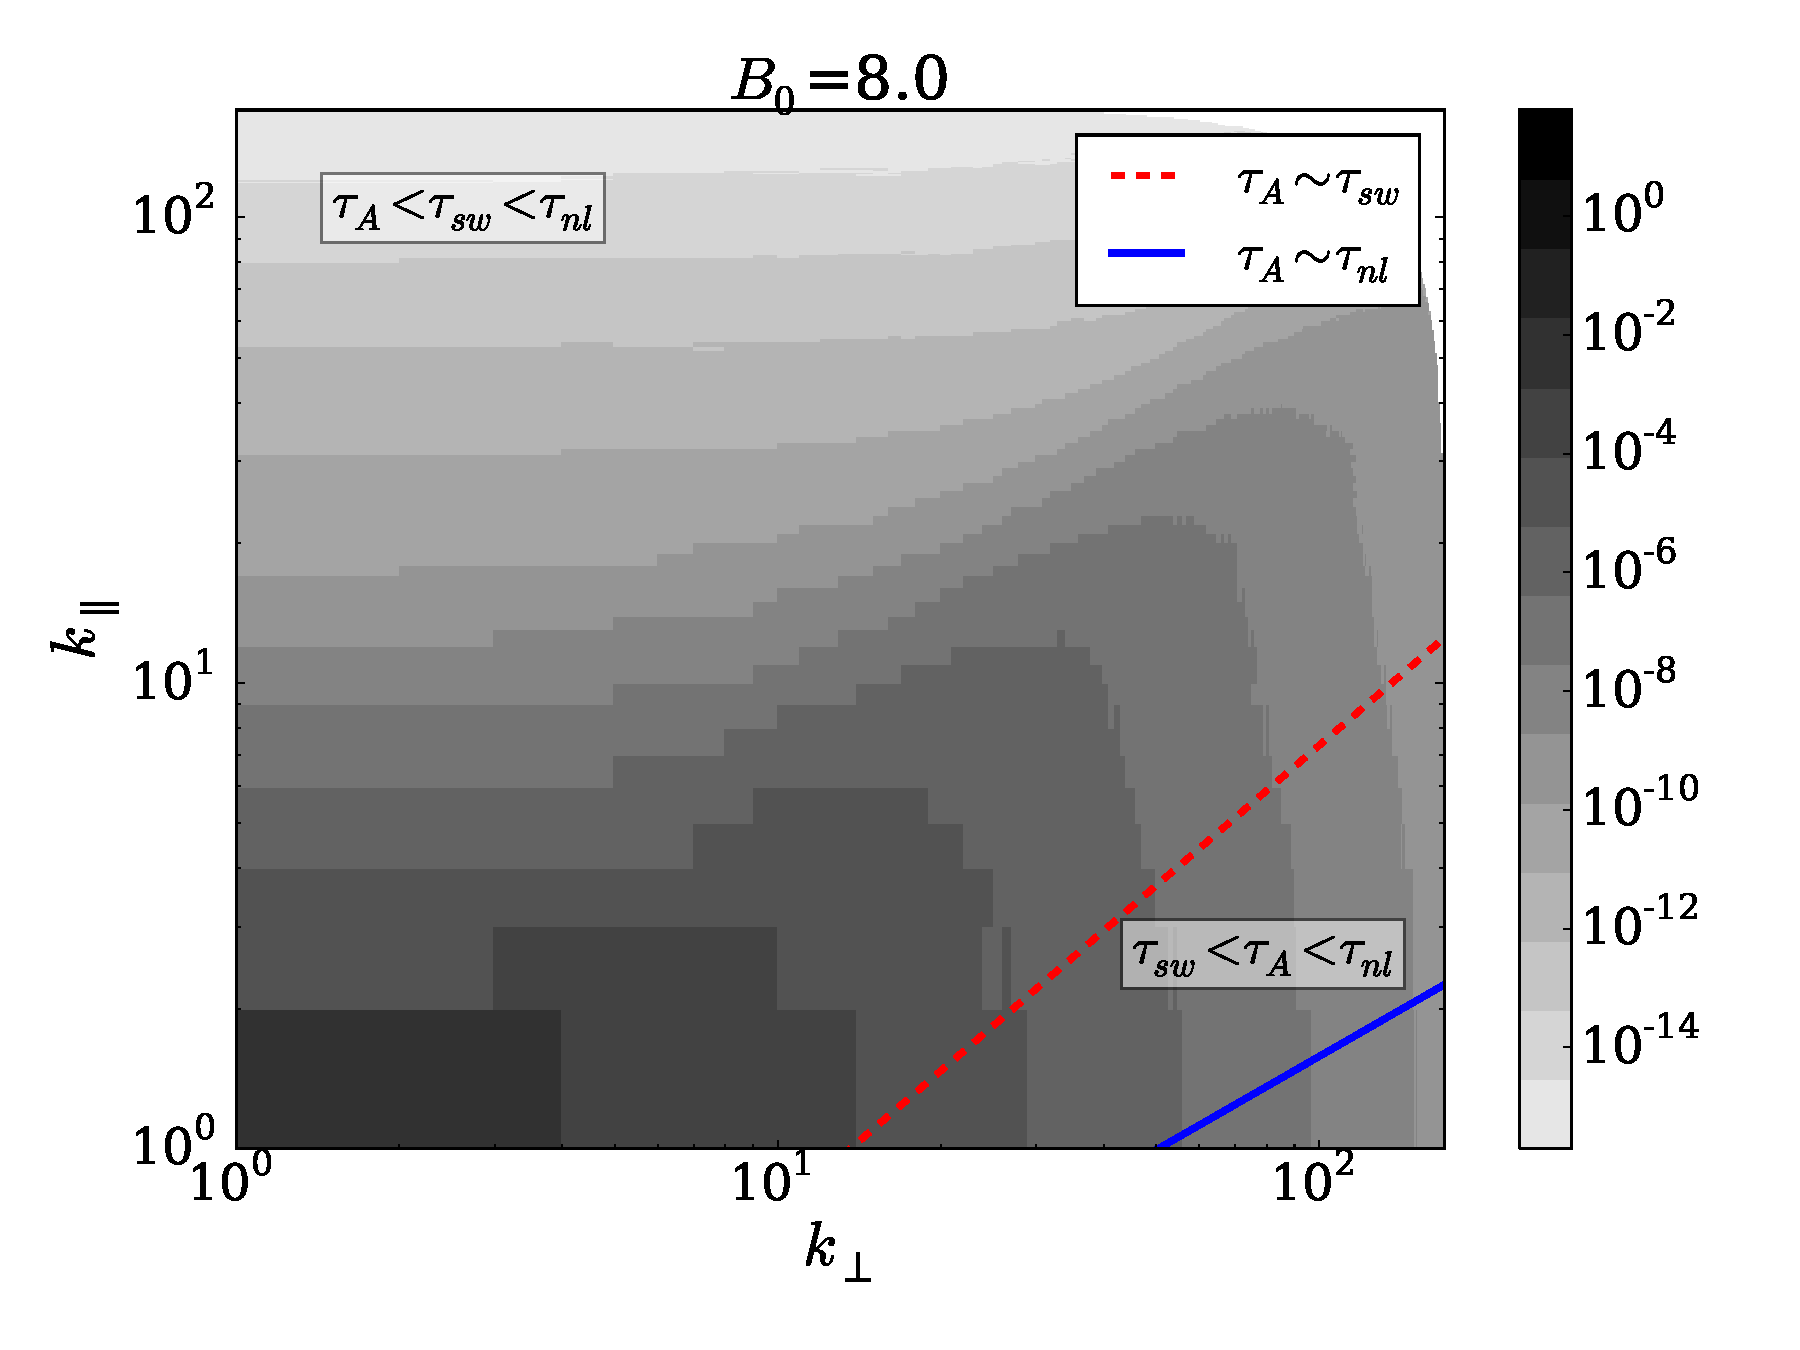
\includegraphics[width=0.48\textwidth]{SpatioTemporalSpectra/fig2_B8_log.pdf}}
%  \subfigure[$B_0=8$ in log-log scale]{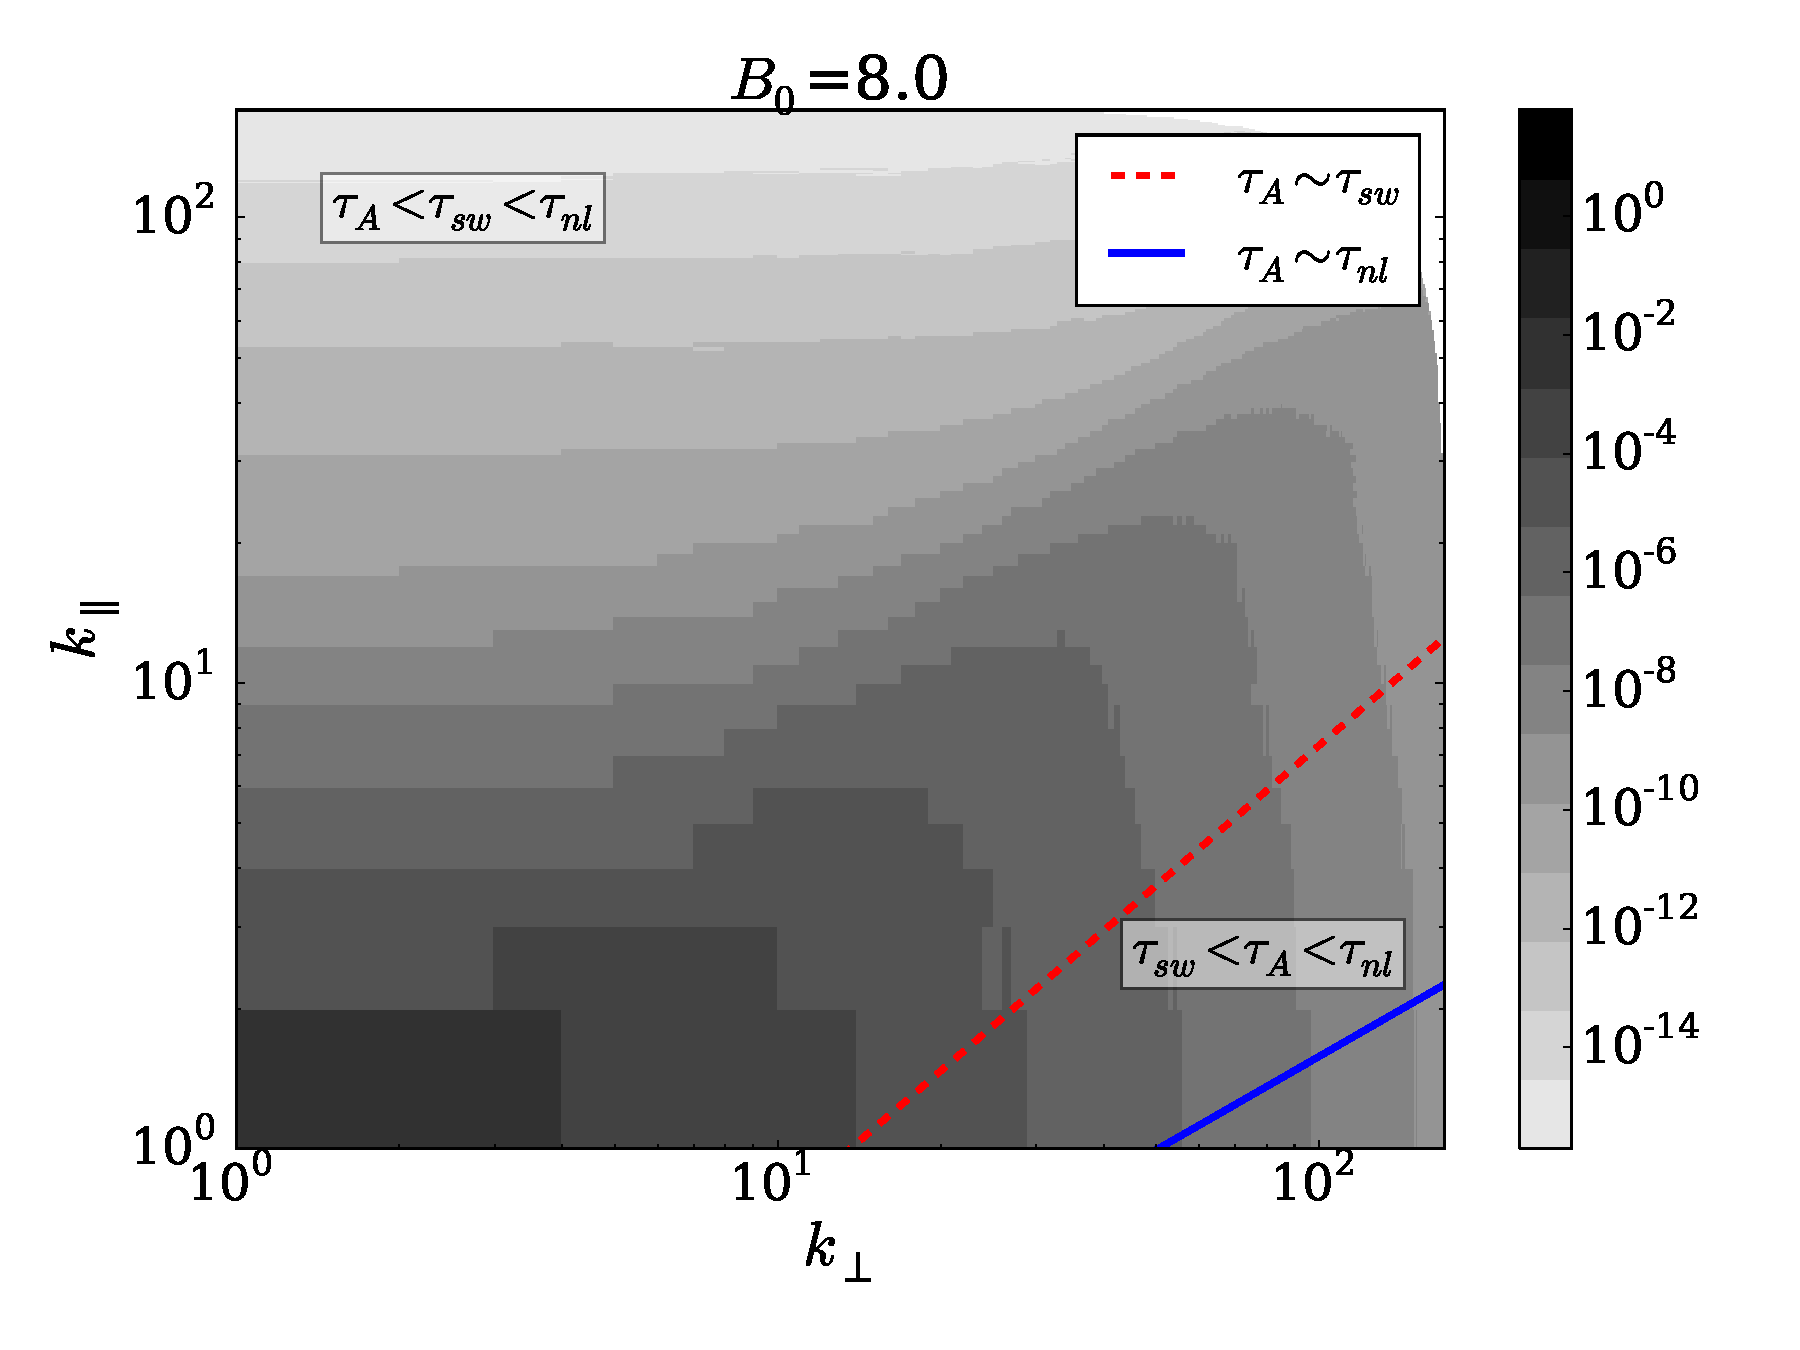
\includegraphics[width=0.45\textwidth]{SpatioTemporalSpectra/fig2_B8_log.eps}}
  \caption{Isocontornos del espectro axisimétrico de energía 
    $e(k_\perp,k_\parallel)$ para $B_0=0$, $1$, $4$ y $8$. Los casos
    con $B_0 = 4$ y $8$ se muestran también en una escala doble logarítmica
    para mostrar con mayor detalle el rango inercial. 
    El color oscuro significa mayor densidad energética (en escala
    logarítmica). Las líneas indican los modos para los que el tiempo de
    \textit{sweeping} o el tiempo no lineal son iguales al tiempo de Alfv\'en.
    Para valores grandes de $B_0$, los isocontornos cambian de forma a
    medida que cruzan cada una de estas líneas. Notar el aumento
    de la anisotropía del espectro a medida que $B_0$ se incrementa, así
    como la mayor superficie cubierta por modos en los que el
    período de Alfv\'en es el tiempo más rápido.}
  \label{fig3-2:isocontourns}
\end{figure*}


\subsection{Espectros espacio-temporales}

Las \cref{fig3-3:B025_bvf_Etot_kperp0,fig3-3:B1_bvf_Etot_kperp0,fig3-3:B8_bvf_Etot_kperp0}
(correspondientes a las simulaciones con $B_0=0.25$, $1$ y $8$,
respectivamente) muestran el espectro en función del vector de onda y
la frecuencia, $E(\vec{k},\omega)/E(\vec{k})$, para modos $\vec{k}$
con $k_\perp = 0$, donde
\begin{equation}
  E(\vec{k})=\int E(\vec{k},\omega)d\omega
\end{equation}
es el espectro de la energía total. Con esta elección para la
normalización, resultan más claramente visibles las frecuencias que
concentran la mayor cantidad de energía para cada $\vec{k}$. Para
$B_0=0.25$ (\cref{fig3-3:B025_bvf_Etot_kperp0}) observamos una clara
dispersión de la energía por debajo de la línea de la relación de
\textit{sweeping} (i.e., vemos excitaciones en todos los modos con frecuencias
iguales o menores que $\omega = v_{rms} k_\parallel$, indicando que
las estructuras de escalas pequeñas están siendo advectadas por todas
las velocidades iguales o menores a $v_{rms}$).  También es observable
para valores pequeños de $k_\parallel$ una acumulación débil cerca de
la relación de dispersión de Alfvén $\omega = B_0 k_\parallel$, aunque
el amplio espectro en el dominio de las frecuencias sugiere que el
\textit{sweeping} es dominante en este caso.

Al incrementar el campo medio a $B_0=1$
(\cref{fig3-3:B1_bvf_Etot_kperp0}), parte de la energía se concentra
por encima de la línea de \textit{sweeping}, y comienza a seguir la
relación de dispersión de Alfvén, aunque el espectro continúa siendo
muy amplio en las frecuencias, con la mayor parte de la energía por
debajo de la relación de \textit{sweeping}.  Este comportamiento
cambia drásticamente para valores más altos de $B_0$.  En
la \cref{fig3-3:B8_bvf_Etot_kperp0} ($B_0=8$), podemos ver que la
energía claramente se concentra alrededor de la relación de dispersión
de las ondas de Alfvén, con un pico de concentración para modos con
hasta $k_\parallel \approx 10$, para posteriormente dispersarse hacia
la relación de \textit{sweeping} para números de onda más grandes.
Notar que este comportamiento indica una competición entre el tiempo
magnetohidrodinámico de \textit{sweeping} y el tiempo de Alfvén, con
este último resultando dominante a grandes escalas para valores de
$B_0$ grandes. Estos resultados respaldan y mejoran los obtenidos por
\cite{dmitruk_waves_2009}, y son compatibles para números de onda
pequeños y $B_0$ grande con los obtenidos recientemente por
\cite{meyrand_direct_2016, meyrand_weak_2015}. En particular, 
\cite{meyrand_direct_2016} también reporta una transición de un
espectro ondular estrecho a un espectro más amplio, aunque la escala y
el mecanismo responsable para esta transición no fue estudiado. Como
confirmaremos en la próxima sección a partir de las funciones de
descorrelación, la competencia entre los tiempos de \textit{sweeping}
y de Alfvén como el tiempo de descorrelación dominante es la
responsable del cambio observado en el comportamiento del espectro.

\begin{figure}
  \centering 
  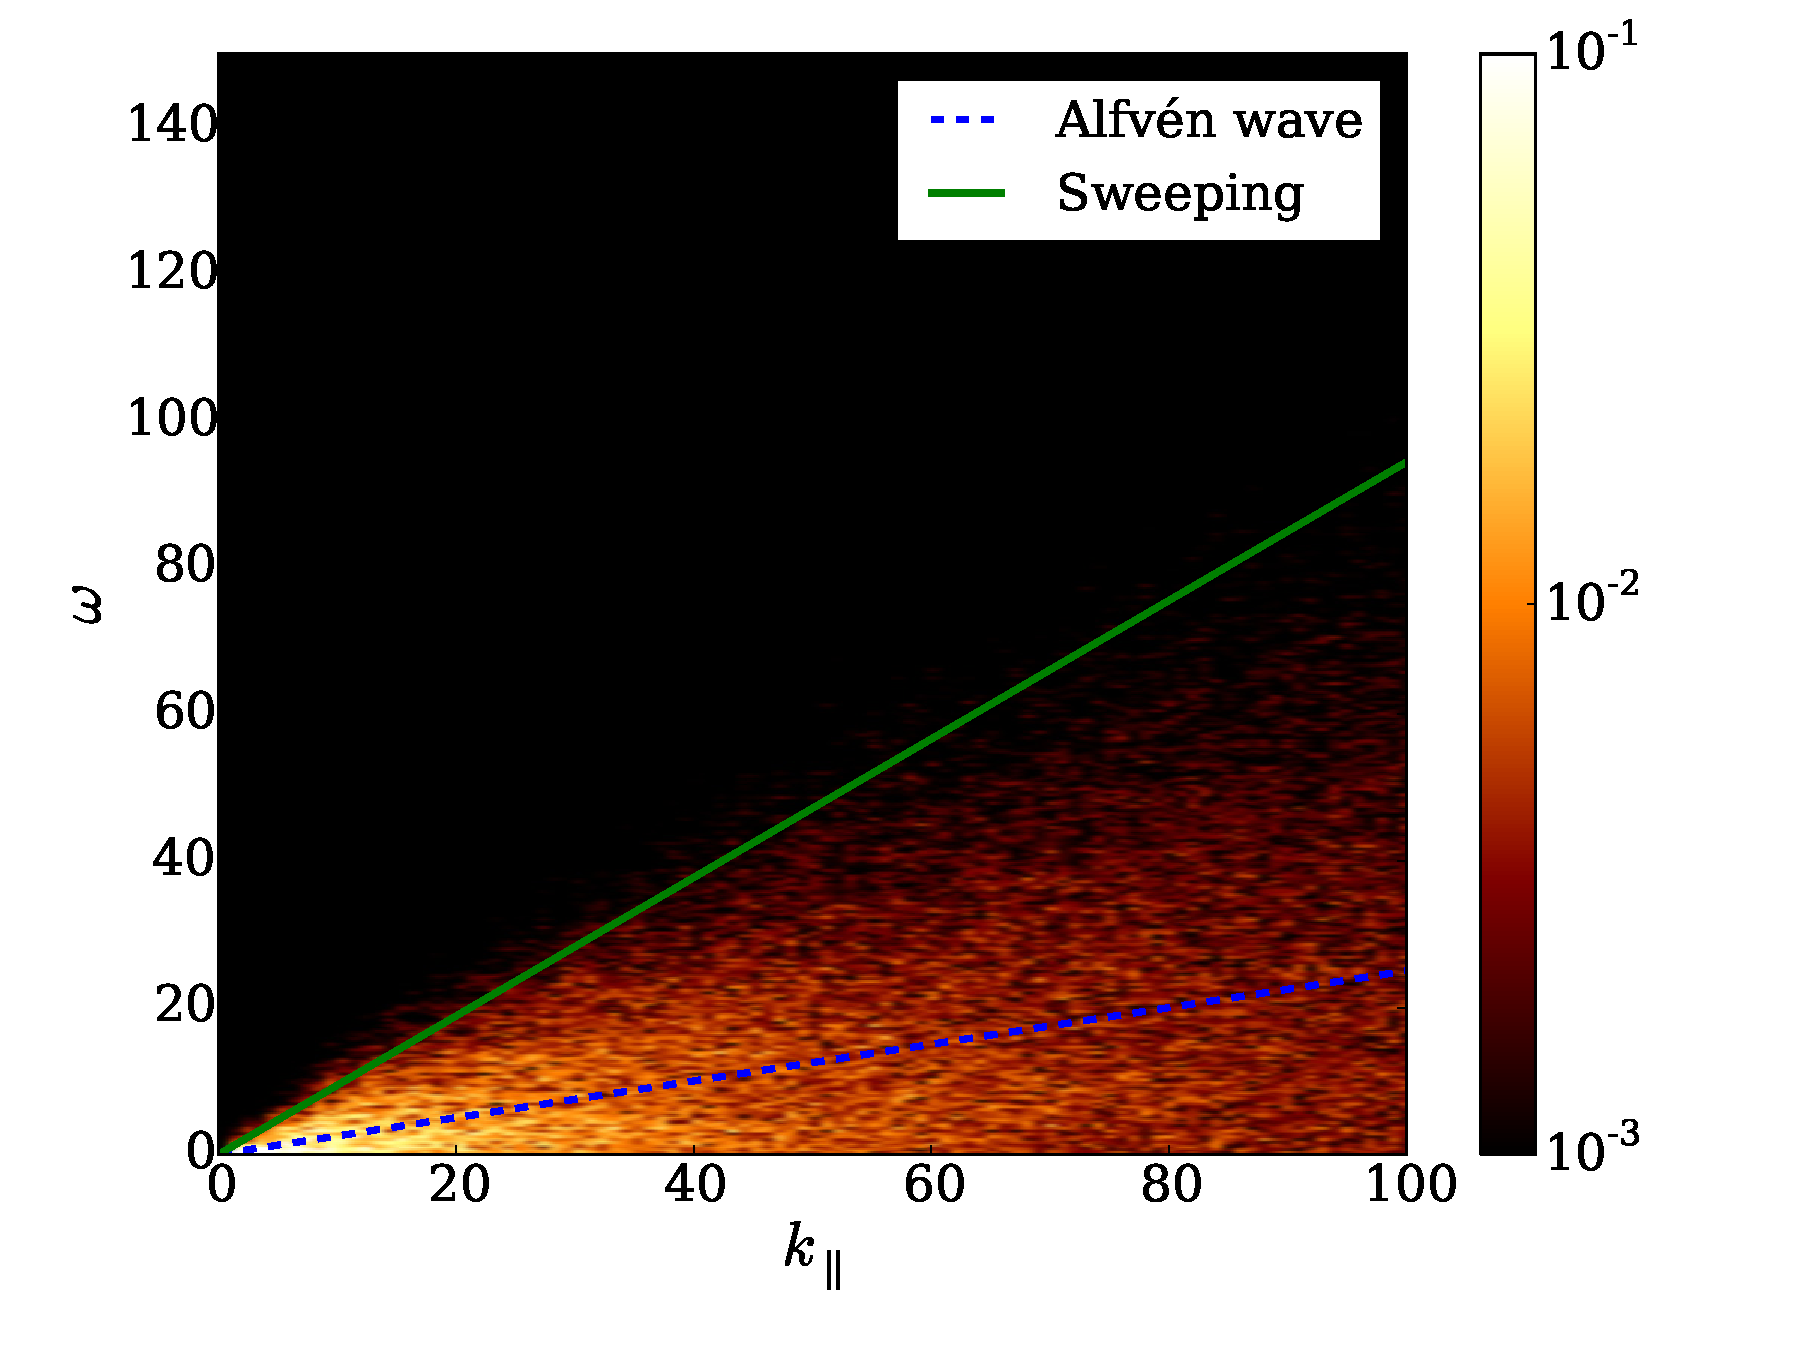
\includegraphics[width=.65\columnwidth]{SpatioTemporalSpectra/fig3_B025_Etot-eps-converted-to.pdf}
  \caption{Espectro normalizado en función del vector de onda y la frecuencia
    $E(\vec{k}, \omega)/E(\vec{k})$ para la simulación con
    $\vec{B_0}=0.25$, para modos con $k_\perp=0$, y en consecuencia en
    función de $k_\parallel$. Las regiones más claras indican mayor
    densidad energética. El espectro corresponde a la transformada de
    Fourier en tiempo y espacio de los campos, por lo que la
    acumulación de energía en modos cercanos a la relación de
    dispersión de Alfv\'en o en los modos debajo de la curva
    de \textit{sweeping} indica el dominio de un efecto físico (i.e.,
    de su frecuencia asociada) en la dinámica del plasma a una dada
    escala $\sim 1/k_\parallel$. La línea discontinua azul indica la
    relación de dispersión de las ondas de Alfv\'en, mientras que la
    línea continua verde marca la relación de \textit{sweeping}. Se
    observa una amplia excitación de modos para los casos con
    $\omega \leq v_{rms} k_\parallel$ (\textit{sweeping}), mientras
    que sobre la relación $\omega=B_0 k_\parallel$ (Alfv\'en) sólo se
    observa una pequeña acumulación de energía para valores pequeños
    de $k_\parallel$.}
  \label{fig3-3:B025_bvf_Etot_kperp0}
\end{figure}

\begin{figure}
  \centering
  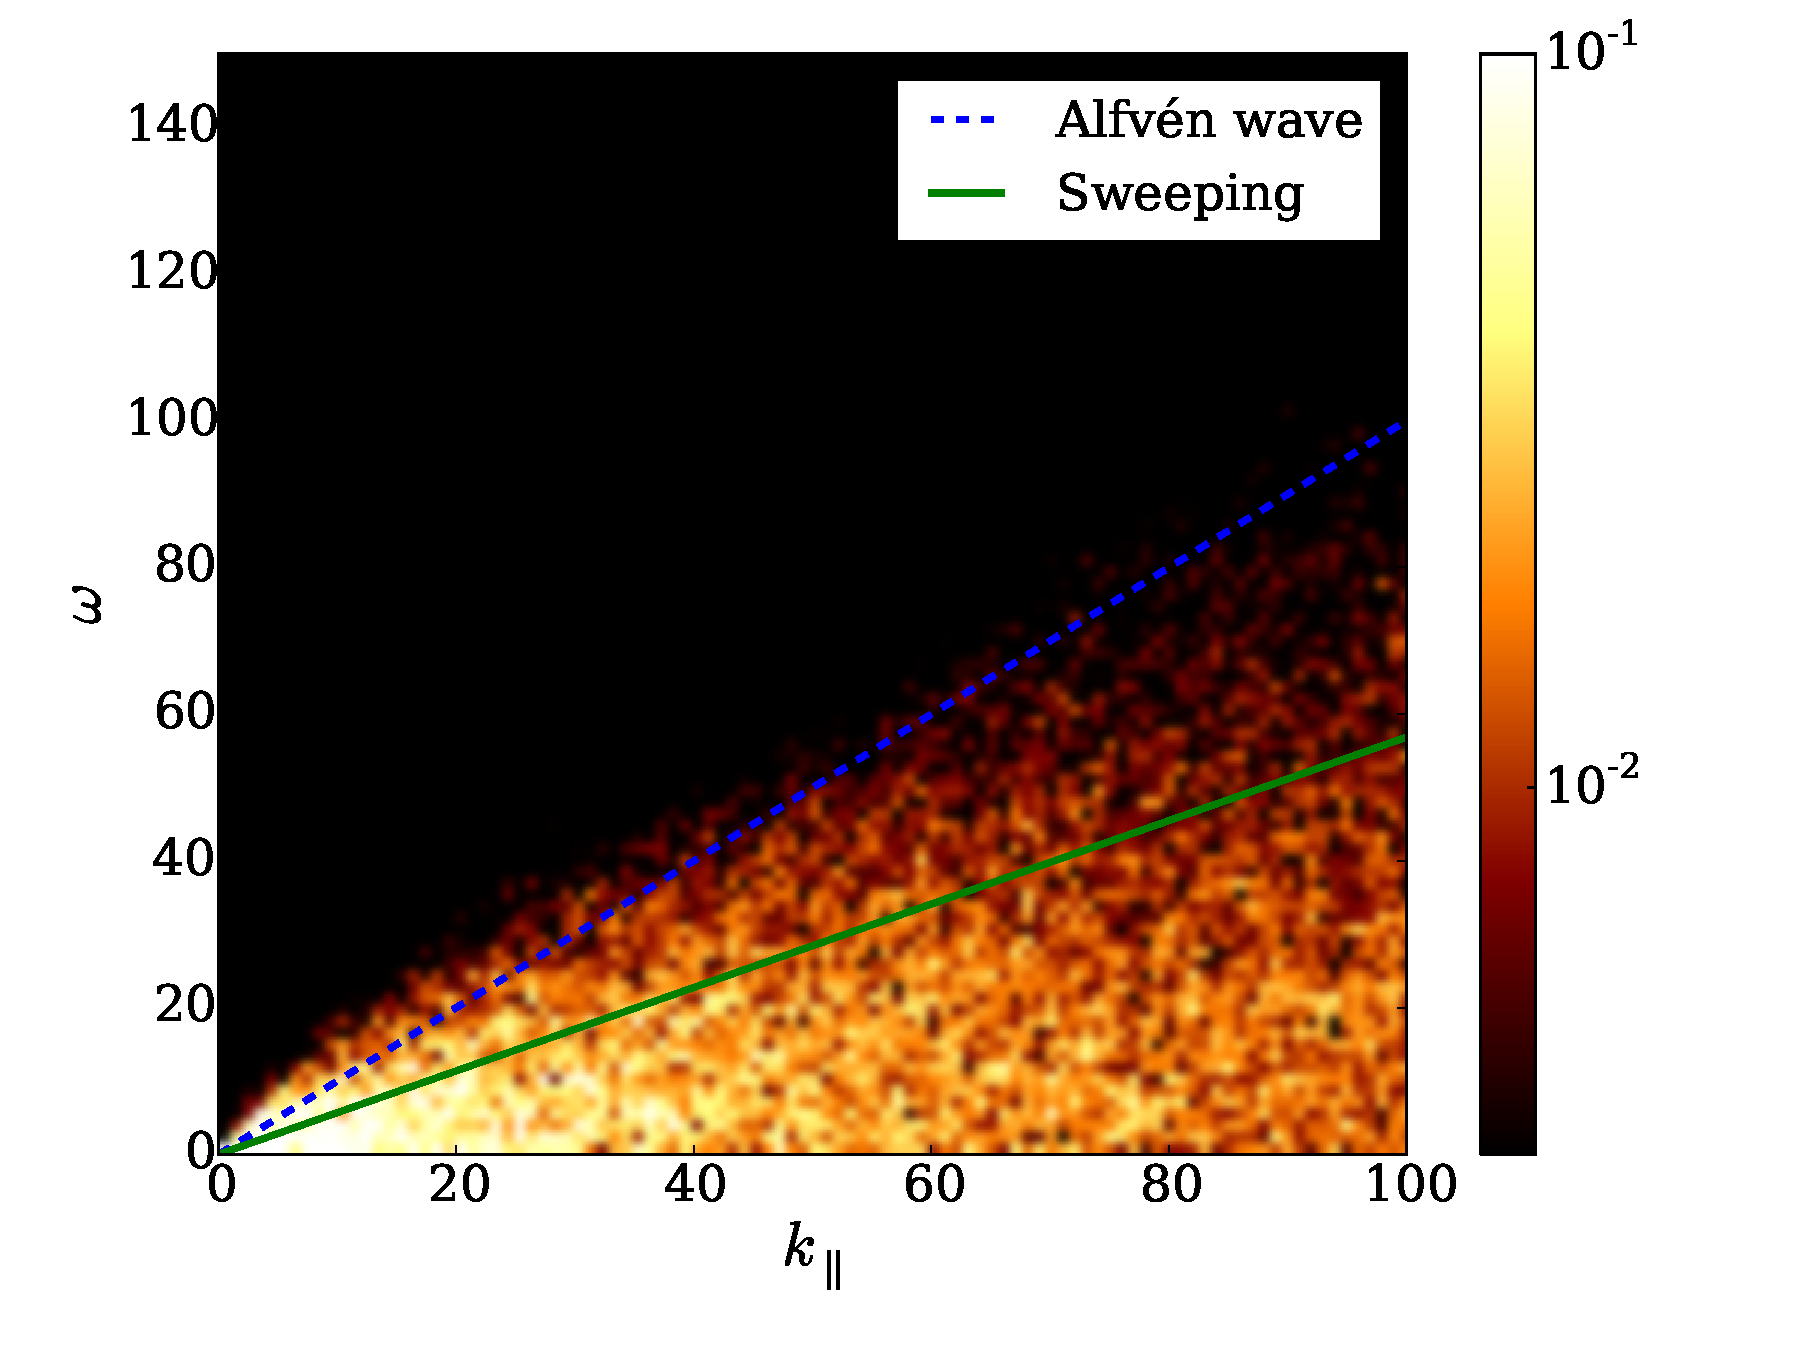
\includegraphics[width=.65\columnwidth]{SpatioTemporalSpectra/fig3_B1_Etot-eps-converted-to.pdf}
  \caption{Espectro normalizado en función del vector de onda y la frecuencia
    $E(\vec{k}, \omega)/E(\vec{k})$ para la simulación con
    $\vec{B_0}=1$, para modos con $k_\perp=0$, y en consecuencia en
    función de $k_\parallel$ y $\omega$. Las regiones más claras indican mayor
    densidad energética. La línea discontinua azul indica la
    relación de dispersión de las ondas de Alfv\'en, mientras que la
    línea continua verde marca la relación de \textit{sweeping}.}
  \label{fig3-3:B1_bvf_Etot_kperp0}
\end{figure}

\begin{figure}
  \centering
  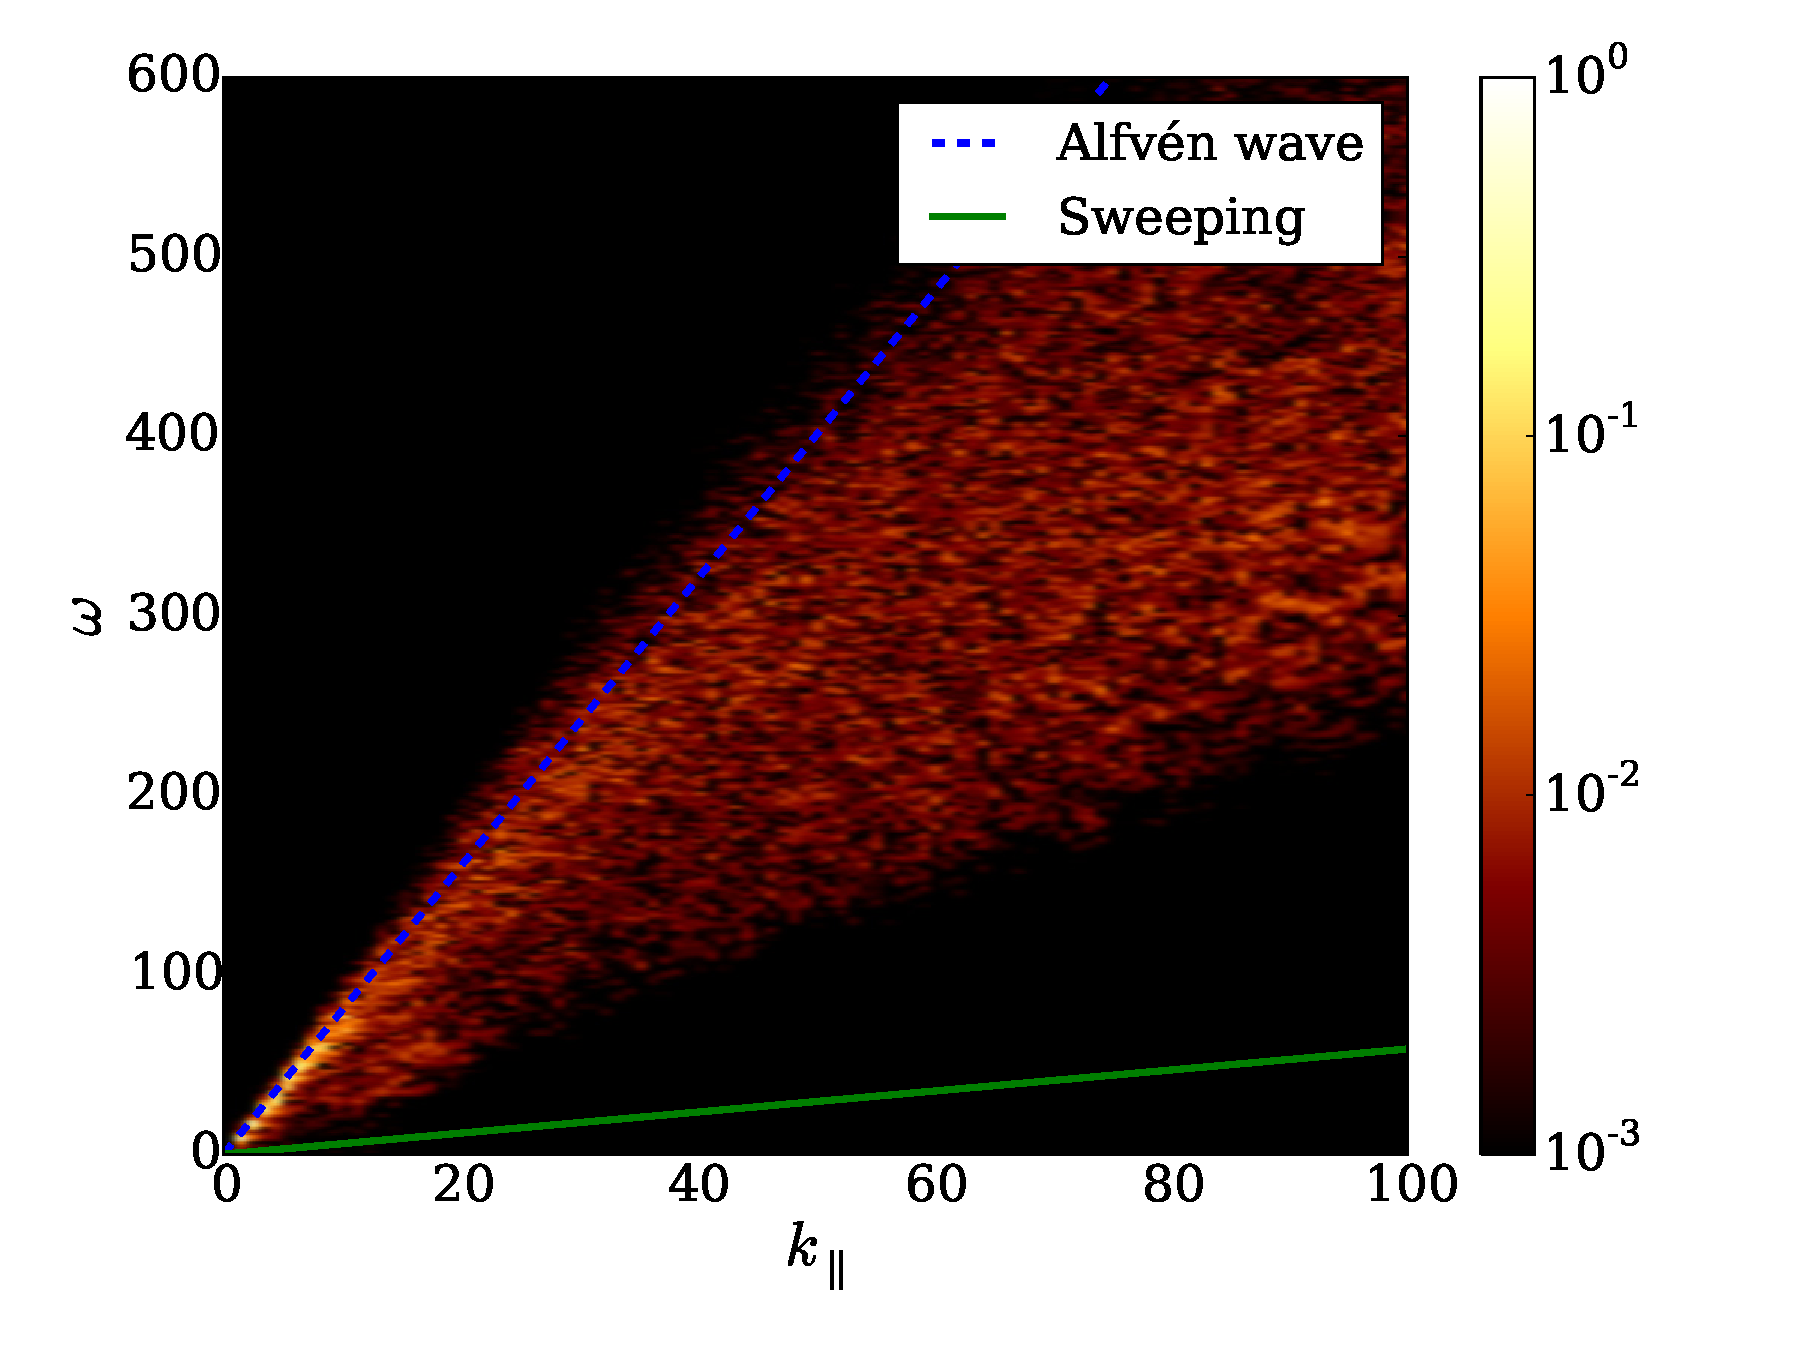
\includegraphics[width=.65\columnwidth]{SpatioTemporalSpectra/fig3_B8_Etot-eps-converted-to.pdf}
  \caption{Espectro normalizado en función del vector de onda y la frecuencia
    $E(\vec{k}, \omega)/E(\vec{k})$ para la simulación con
    $\vec{B_0}=8$, para modos con $k_\perp=0$, y en consecuencia en
    función de $k_\parallel$ y $\omega$. Las regiones más claras indican mayor
    densidad energética. La línea discontinua azul indica la
    relación de dispersión de las ondas de Alfv\'en, mientras que la
    línea continua verde marca la relación de \textit{sweeping}.
    Notar que en este caso, la mayor cantidad de energía se concentra
    en una región angosta cercana a la relación de dispersión de ondas
    hasta $k_\parallel \approx 10$, correspondiente a excitaciones
    Alfv\'enicas.}
  \label{fig3-3:B8_bvf_Etot_kperp0}
\end{figure}


\begin{figure}
  \centering
  \subfigure[$\Gamma(k_\perp=0,k_\parallel=k_0,\tau)$]{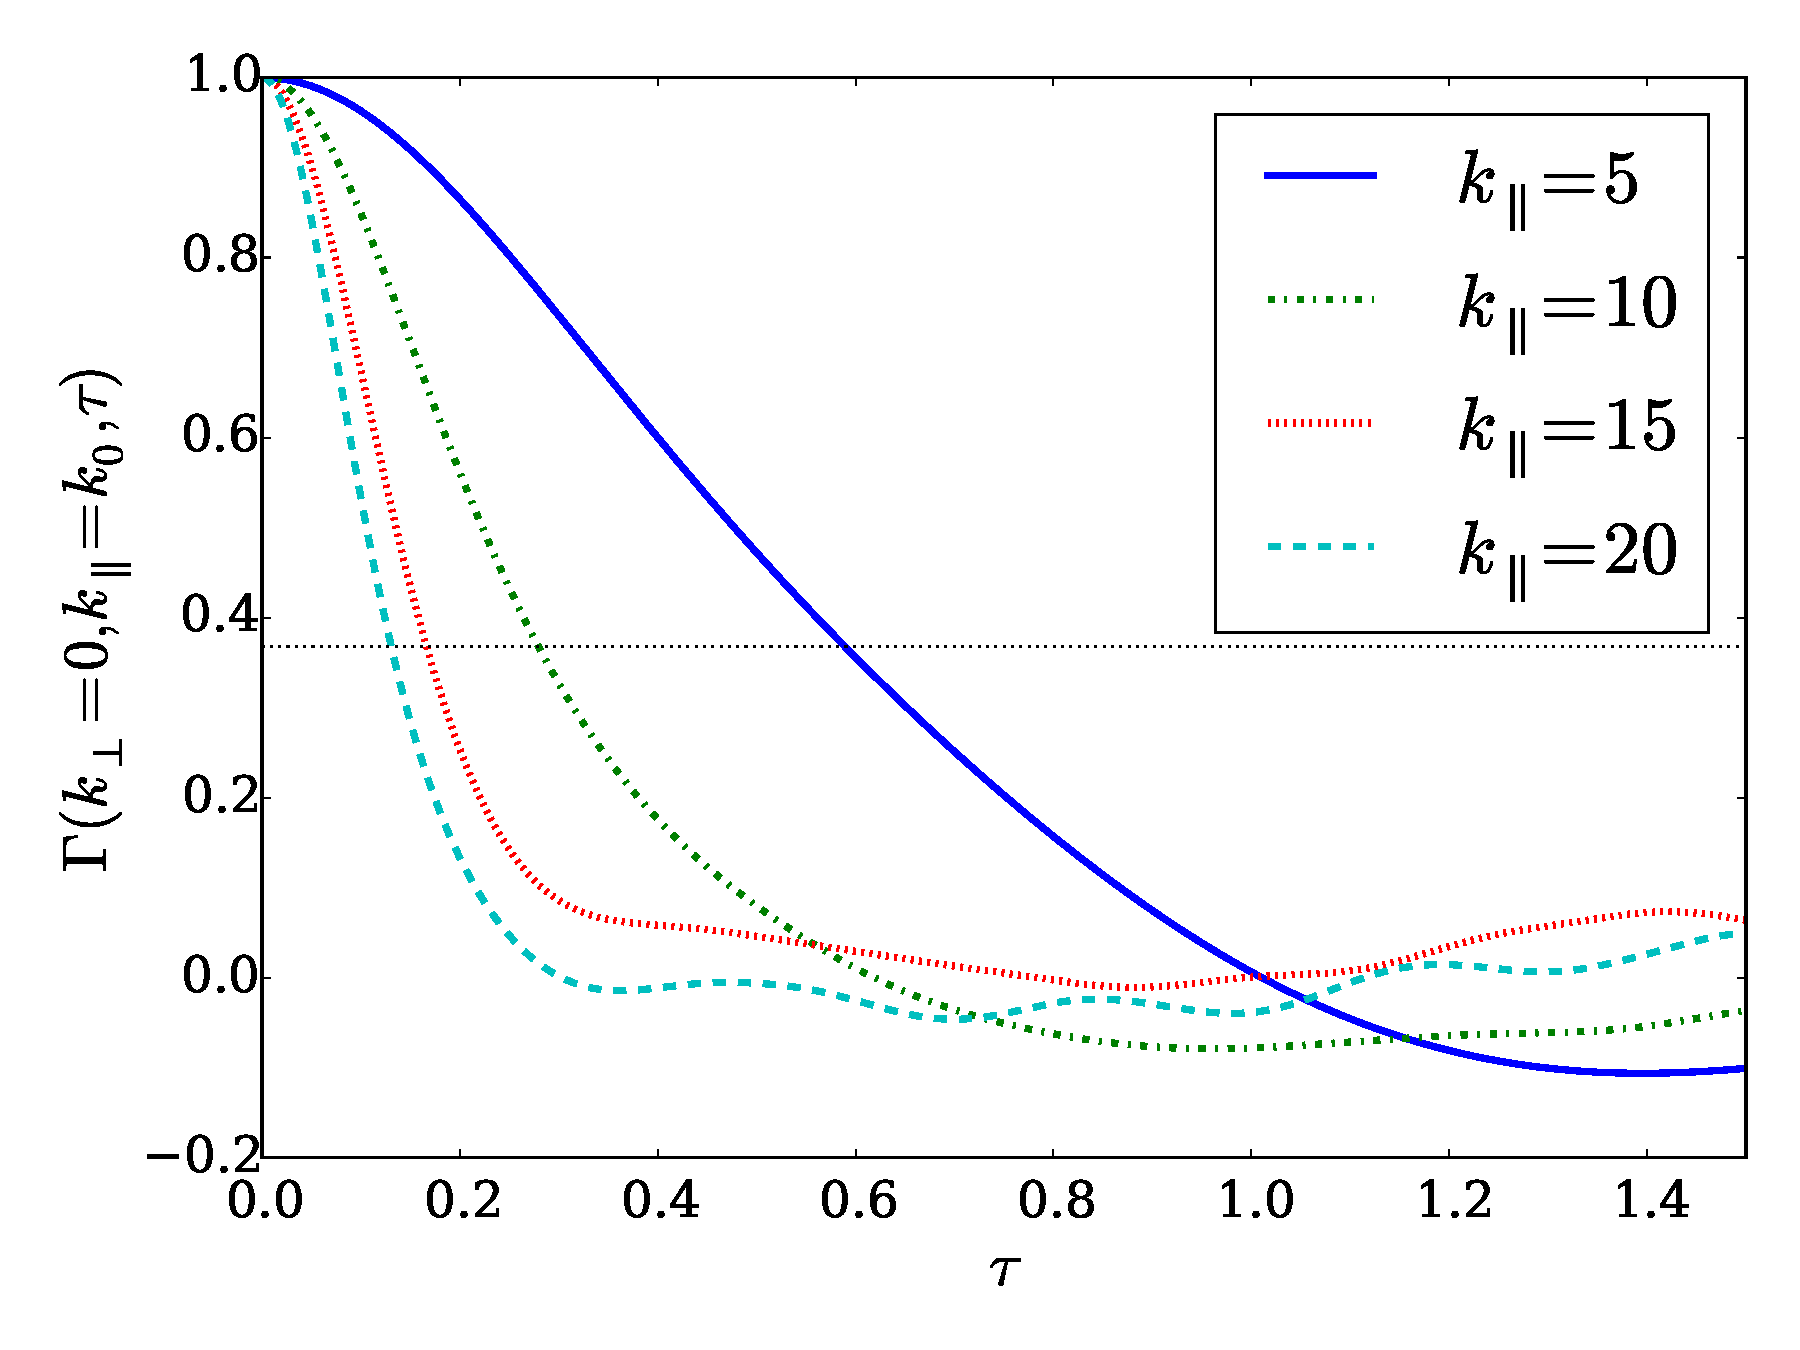
\includegraphics[width=0.7\columnwidth]{SpatioTemporalSpectra/fig4_B1_b_kperp-eps-converted-to.pdf}}

  \subfigure[$\Gamma(k_\perp=k_0,k_\parallel=0,\tau)$]{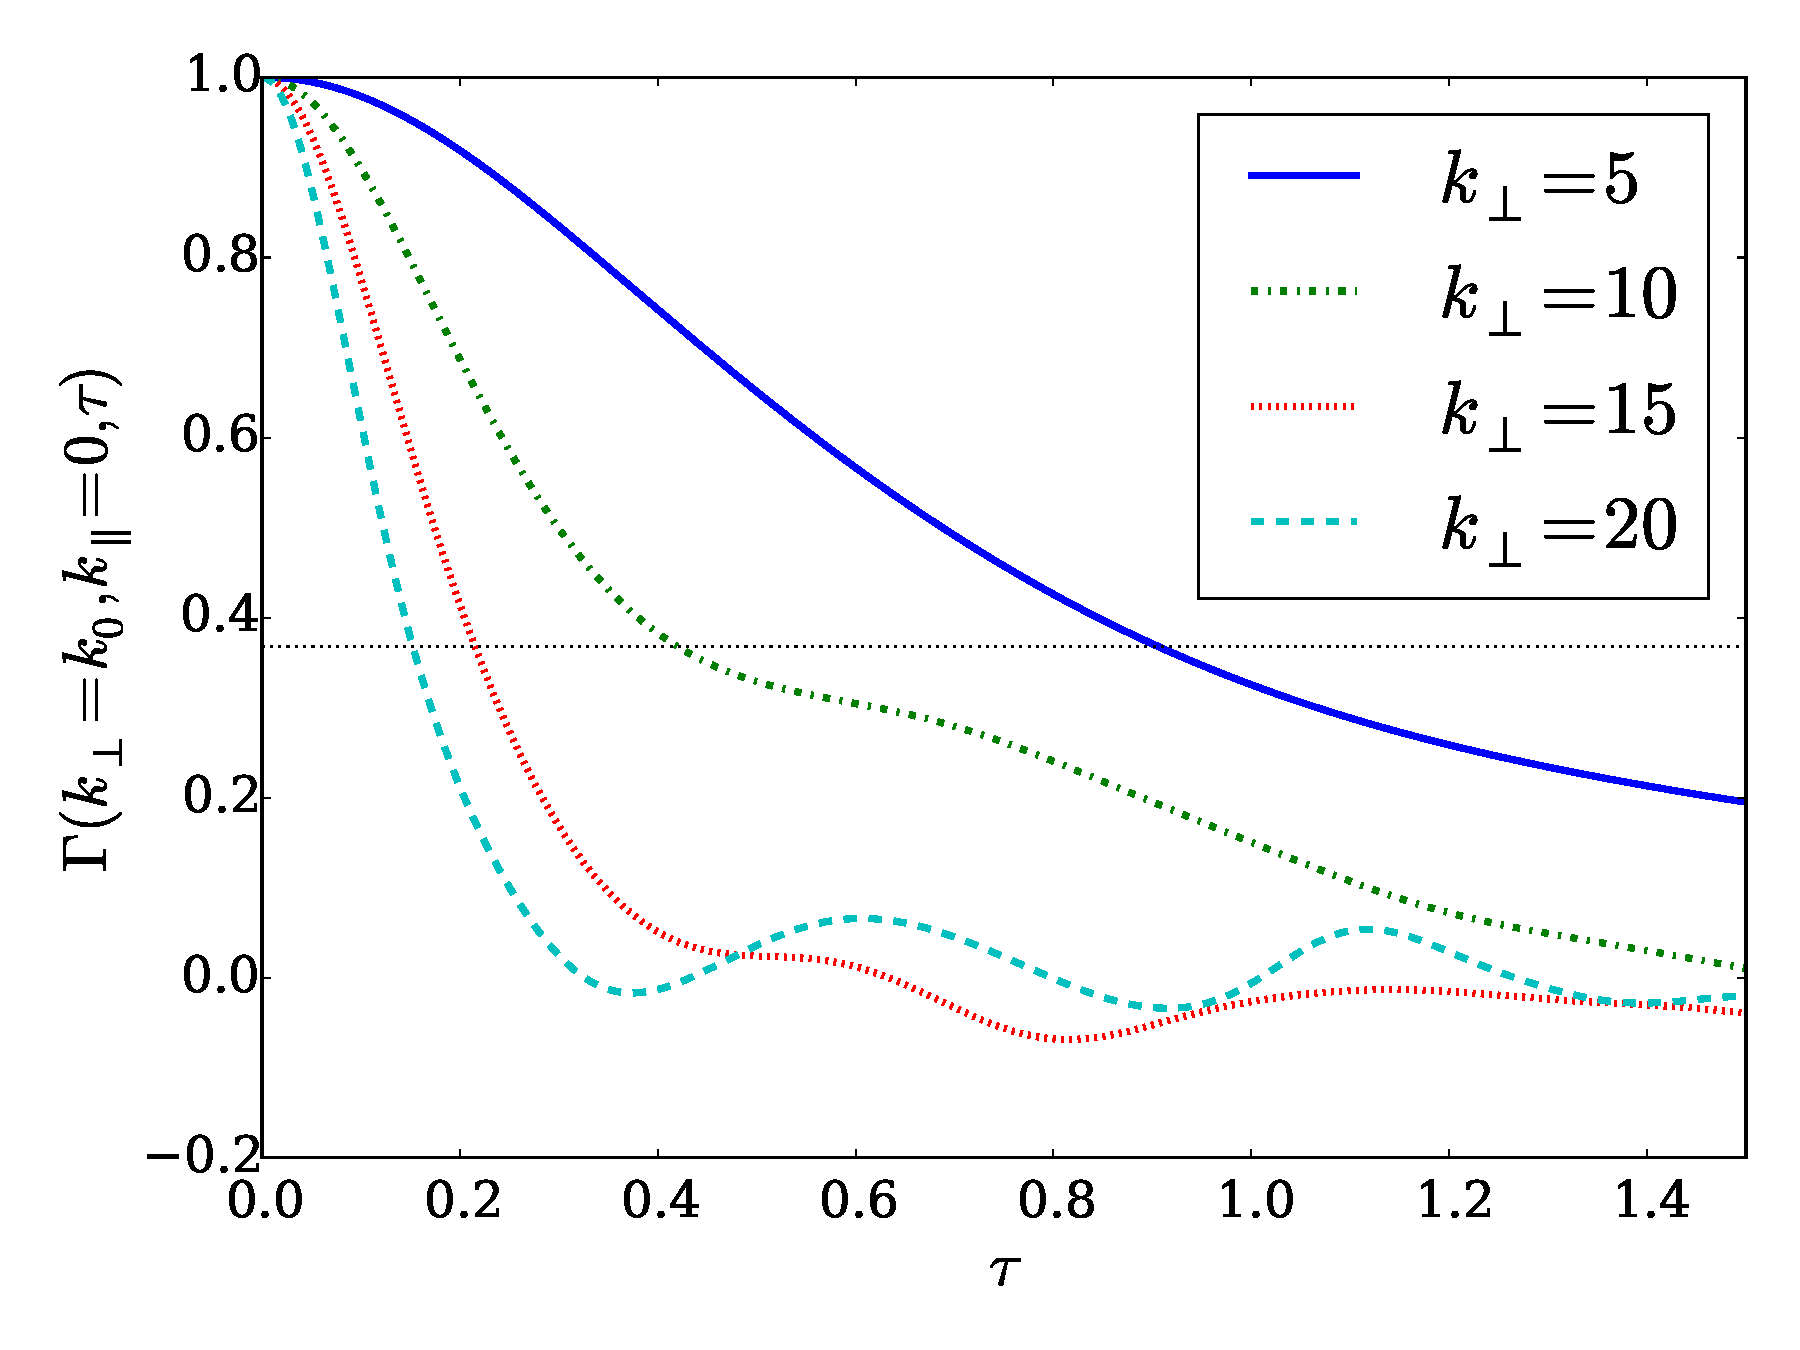
\includegraphics[width=0.7\columnwidth]{SpatioTemporalSpectra/fig4_B1_b_kpara-eps-converted-to.pdf}}
  \caption{Funciones de correlación
    $\Gamma(k_\perp=0,k_\parallel=k_0,\tau)$ y
    $\Gamma(k_\perp=k_0,k_\parallel=0,\tau)$ en función del tiempo de
    retraso $\tau$, para $k_0=5$, $10$, $15$, y $20$, en la simulación con
    $B_0=1$. El valor de $\tau$ para el cual $\Gamma=1/e$ (línea punteada
    horizontal) corresponde al tiempo de descorrelación $\tau_D$ para
    cada valor de $\vec{k}$.}
  \label{fig3-4:B1_bvf_b_kperp/kpara0}
\end{figure}


\subsection{Funciones de correlación y tiempos de descorrelación}

Con el fin de discernir entre los diferentes fenómenos (y escalas de
tiempo relevantes) que actúan en la turbulencia magnetohidrodinámica,
estudiamos las funciones de correlación $\Gamma(\vec{k},\tau)$, como
se explicó en detalle previamente en la sección
\ref{sec3:Wfspectrum_and_Gamma}. Dado que nos enfocamos en la
turbulencia con un campo magnético guía, utilizamos $\Gamma(k_\perp,
k_\parallel, \tau)$ y consideramos varios valores de $(k_\perp,
k_\parallel)$ para estudiar la descorrelación como función del tiempo
de retraso $\tau$ a diferentes escalas.  En la
\cref{fig3-4:B1_bvf_b_kperp/kpara0}, se muestran las funciones de
correlación $\Gamma(k_\perp=0,k_\parallel=k_0,\tau)$ y
$\Gamma(k_\perp=k_0,k_\parallel=0,\tau)$ para diferentes valores de
$k_0$ para el caso del campo magnético externo moderado $B_0=1$. Aquí
podemos ver el comportamiento típico de las funciones de correlación,
con las escalas más grandes ($k$ más pequeños) tomándose un mayor
tiempo para descorrelacionarse. Se encontraron resultados similares
para los otros campos magnéticos externos considerados, $B_0=0$,
$0.25$, $4$ y $8$.

Para entender cuál de los diferentes tiempos (tiempo no lineal,
\textit{sweeping} aleatorio y propagación de Alfvén) está controlando la
descorrelación temporal, necesitamos comparar el tiempo de
descorrelación en las distintas escalas con el comportamiento teórico
esperada para cada proceso físico. Para hacer esto, usamos el hecho de
que el modo con el vector de onda $\vec{k}$ debe estar
descorrelacionada después de un tiempo $\tau_D(\vec{k})$, siguiendo
aproximadamente un decaimiento exponencial
\begin{equation}
\Gamma(\vec{k},\tau) \sim e^{-\tau/\tau_D(\vec{k})}.
\end{equation}
Por simplicidad, evaluamos $\tau_D(\vec{k})$ como el tiempo al cual la
función $\Gamma$ decaía a $1/e$ de su valor inicial.

\begin{figure}
  \centering
  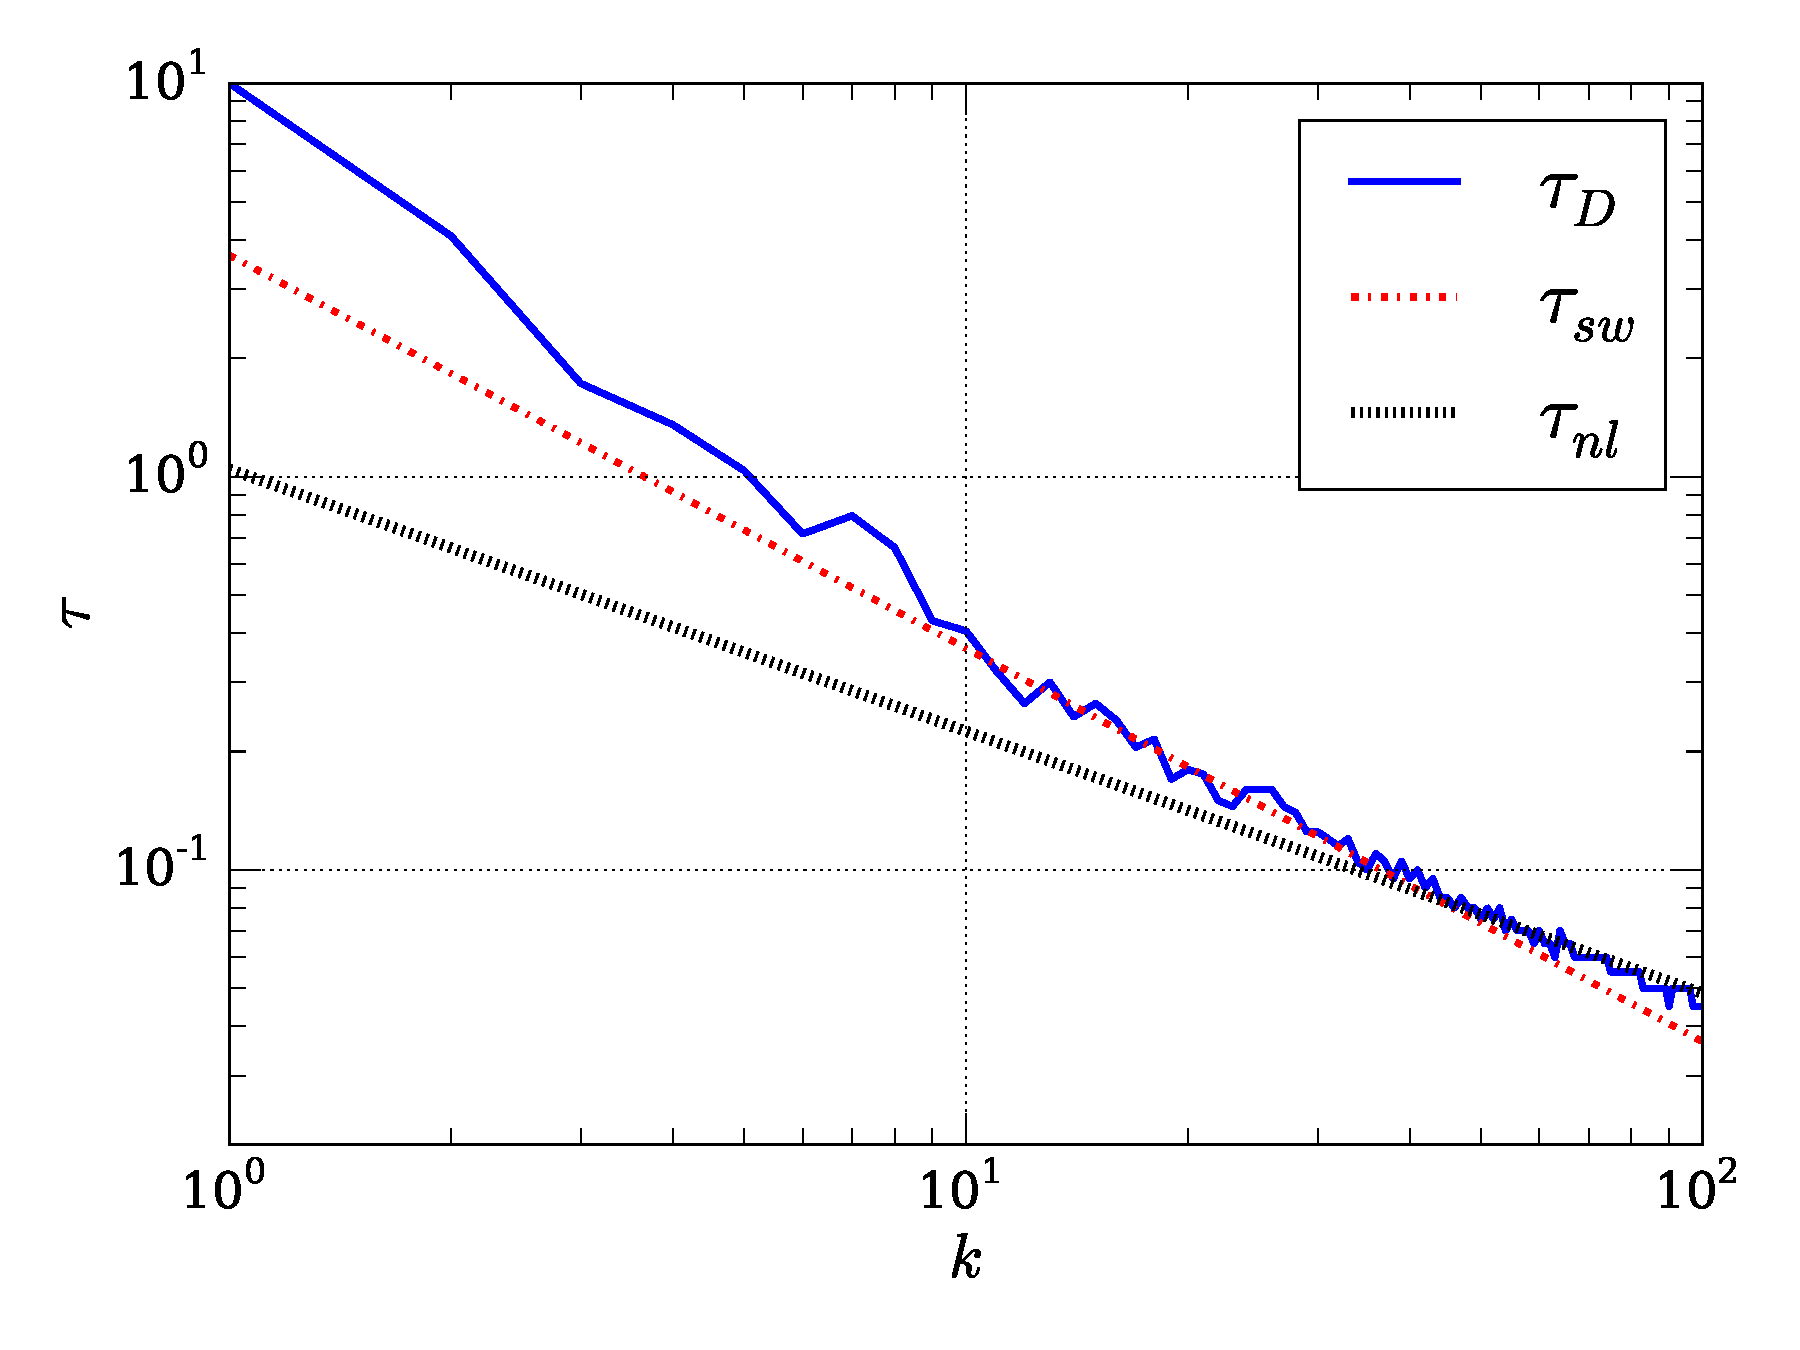
\includegraphics[width=.6\columnwidth]{SpatioTemporalSpectra/fig5_B0_b-eps-converted-to.pdf}
  \caption{Tiempo de descorrelación en función de $k=|\vec{k}|$ para el caso
  isotrópico $B_0=0$. Las líneas rectas indican las predicciones teóricas
  correspondientes al tiempo de \textit{sweeping} y al tiempo no lineal.
  Excepto para los número de onda más grandes, el tiempo de descorrelación
  parece estar dominado por el \textit{sweeping}.}
  \label{fig3-5:B0_bvf_b_kpara_0}
\end{figure}

Como primer ejemplo, la \cref{fig3-5:B0_bvf_b_kpara_0} muestra el tiempo
de descorrelación $\tau_D$ obtenido de $\Gamma(k,\tau)$ en el caso
isotrópico con $B_0=0$.  Podemos ver que la escala del tiempo de
descorrelación se encuentra en buen acuerdo con el tiempo de
\textit{sweeping}, excepto quizás para los números de onda más grandes (menor
escala). Estos resultados son consistentes con los obtenidos
por \cite{servidio_time_2011} en el caso isotrópico.

Como se mencionó anteriormente, en el caso general puede ser difícil
diferenciar entre los efectos de \textit{sweeping} y de la propagación de
Alfvén, pues ambas escalas temporales varían como $k^{-1}$. Sin
embargo, en el caso anisotrópico (i.e., en presencia de un campo
guía), podemos hacer uso del escaleo observado respecto de los números
de onda paralelos y perpendiculares, para así hacer posible la
distinción.  En la \cref{fig3-5:B025_bvf_b_kperp} utilizamos resultados
de la simulación con $B_0=0.25$ para computar los tiempos de
descorrelación para los modos de Fourier en función de $k_\parallel$,
para varios valores fijos de $k_\perp$. Incluso para este caso con un
valor de $B_0$ relativamente pequeño, puede observarse que los tiempos
de descorrelación se encuentran más cerca del valor teórico esperado
del tiempo de \textit{sweeping} que de todos los otros tiempos (tiempo local
no lineal y tiempo Alfvénico). Esto es consistente con el resultado
obtenido a partir del espectro energético respecto del número de onda
y la frecuencia, mostrado previamente en la
\cref{fig3-3:B025_bvf_Etot_kperp0}. En la \cref{fig3-5:B025_bvf_b_kpara}
se muestra una vista complementaria para la misma corrida con
$B_0=0.25$, donde se muestra el tiempo de descorrelación $\tau$ en
función de $k_\perp$ para varios valores fijados de $k_\parallel$. La
conclusión es nuevamente que el tiempo de \textit{sweeping} controla
$\tau_D$ a todas las escalas, salvo las más grandes, ya que sólo para
$k_\perp=0$ y para $k_\parallel$ entre $1$ y $4$ $\tau_D$ se encuentra
más cercano al tiempo de Alfvén.

La tendencia de que el tiempo de descorrelación sea controlado por el
\textit{sweeping} se puede ver nuevamente en la corrida con el campo medio
moderado $B_0=1$. Estos resultados para el tiempo de descorrelación se
muestran en
las \cref{fig3-5:B1_bvf_b_kperp,fig3-5:B1_bvf_b_kpara}. Nuevamente, sólo
para valores pequeños de $k_{\parallel}$ y de $k_{\perp}=0$ el tiempo
de descorrelación se encuentra más cerca del tiempo de Alfvén. Esta
tendencia pudo observarse también en el espectro de la
\cref{fig3-3:B1_bvf_Etot_kperp0}.

\begin{figure}
  \centering
  \subfigure[$k_\perp=0$]{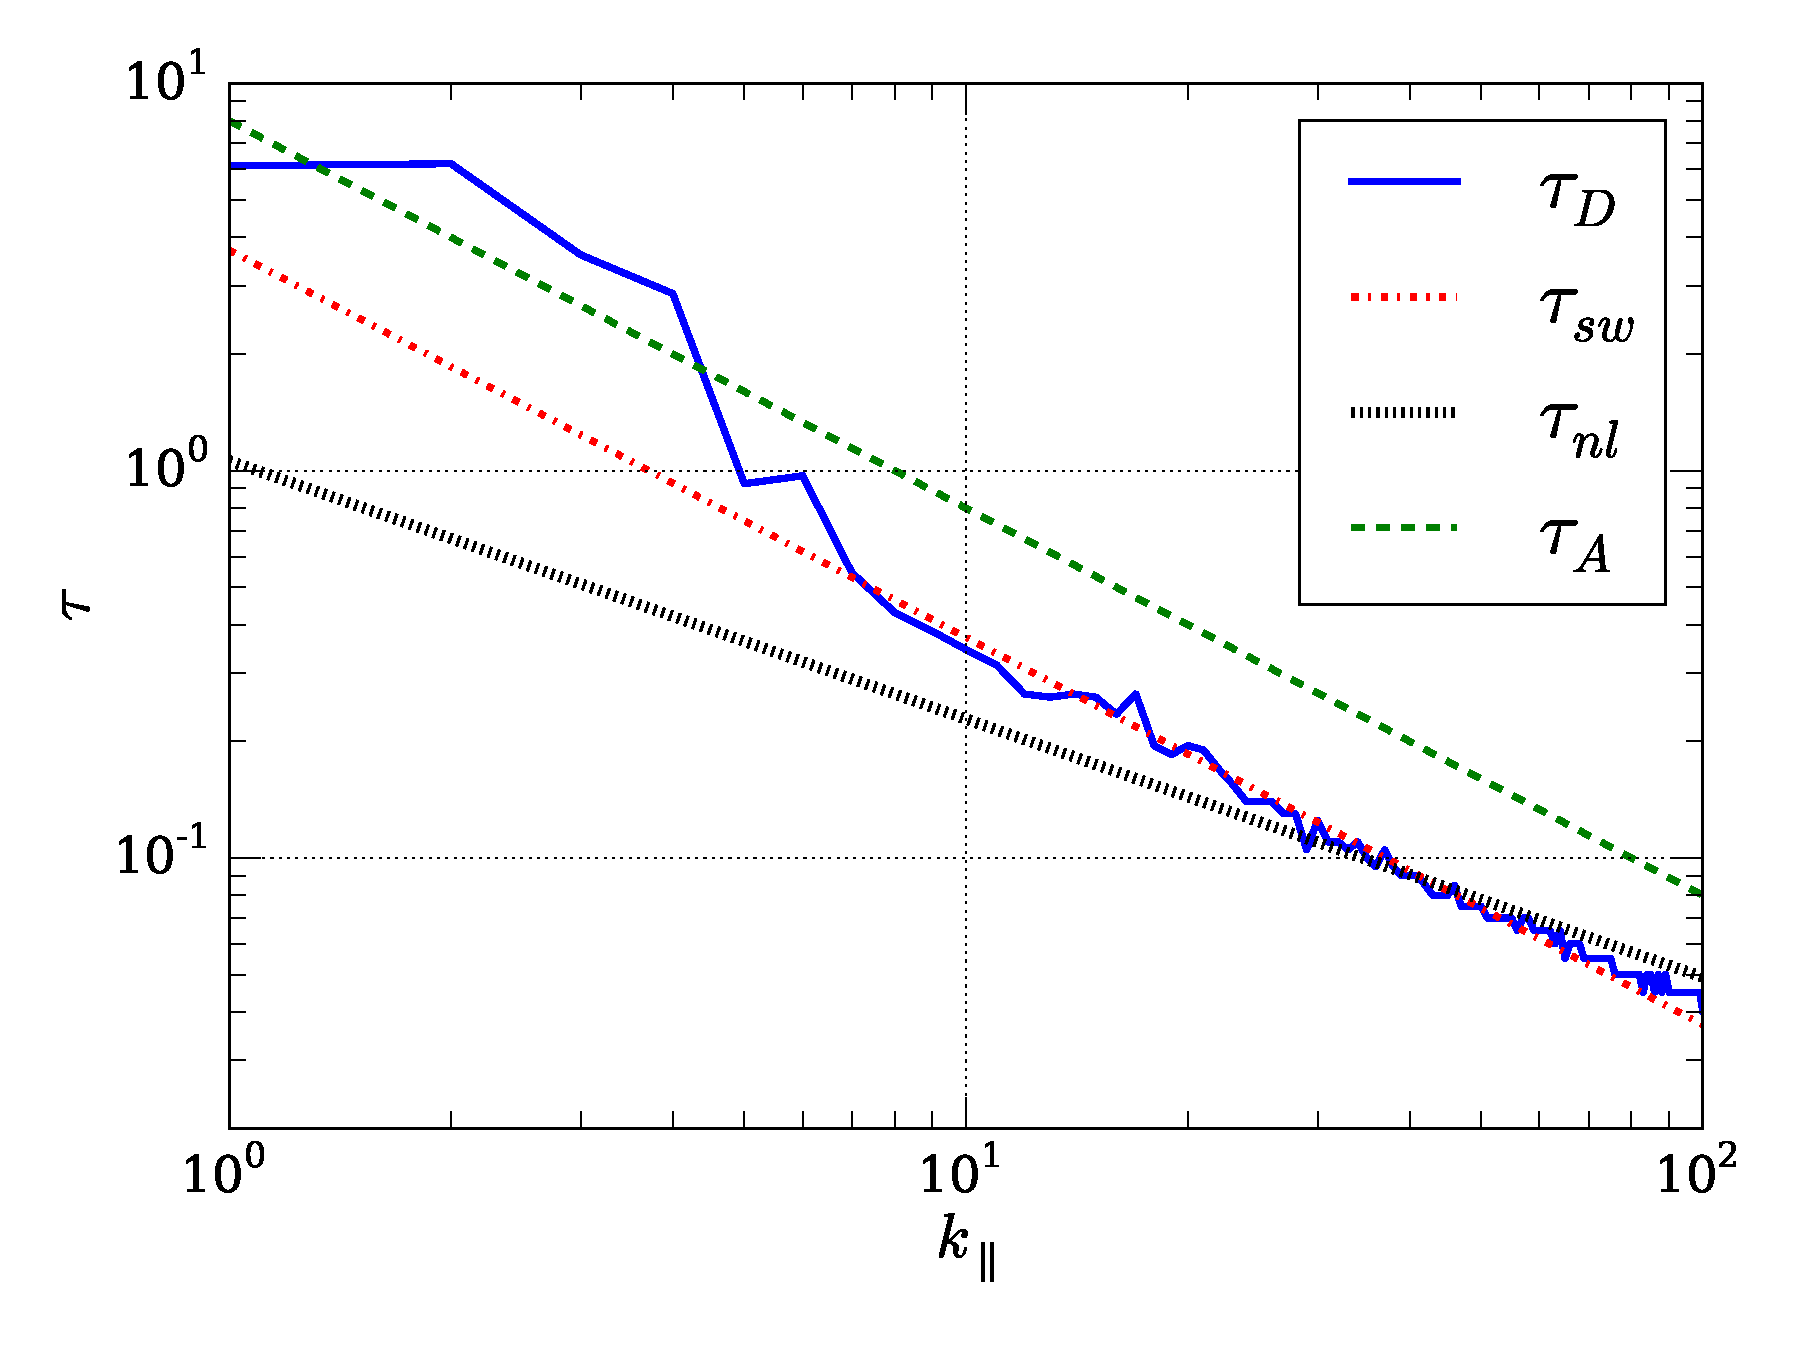
\includegraphics[width=0.49\columnwidth]{SpatioTemporalSpectra/fig5_B025_b_kperp_0-eps-converted-to.pdf}}
  \subfigure[$k_\perp=10$]{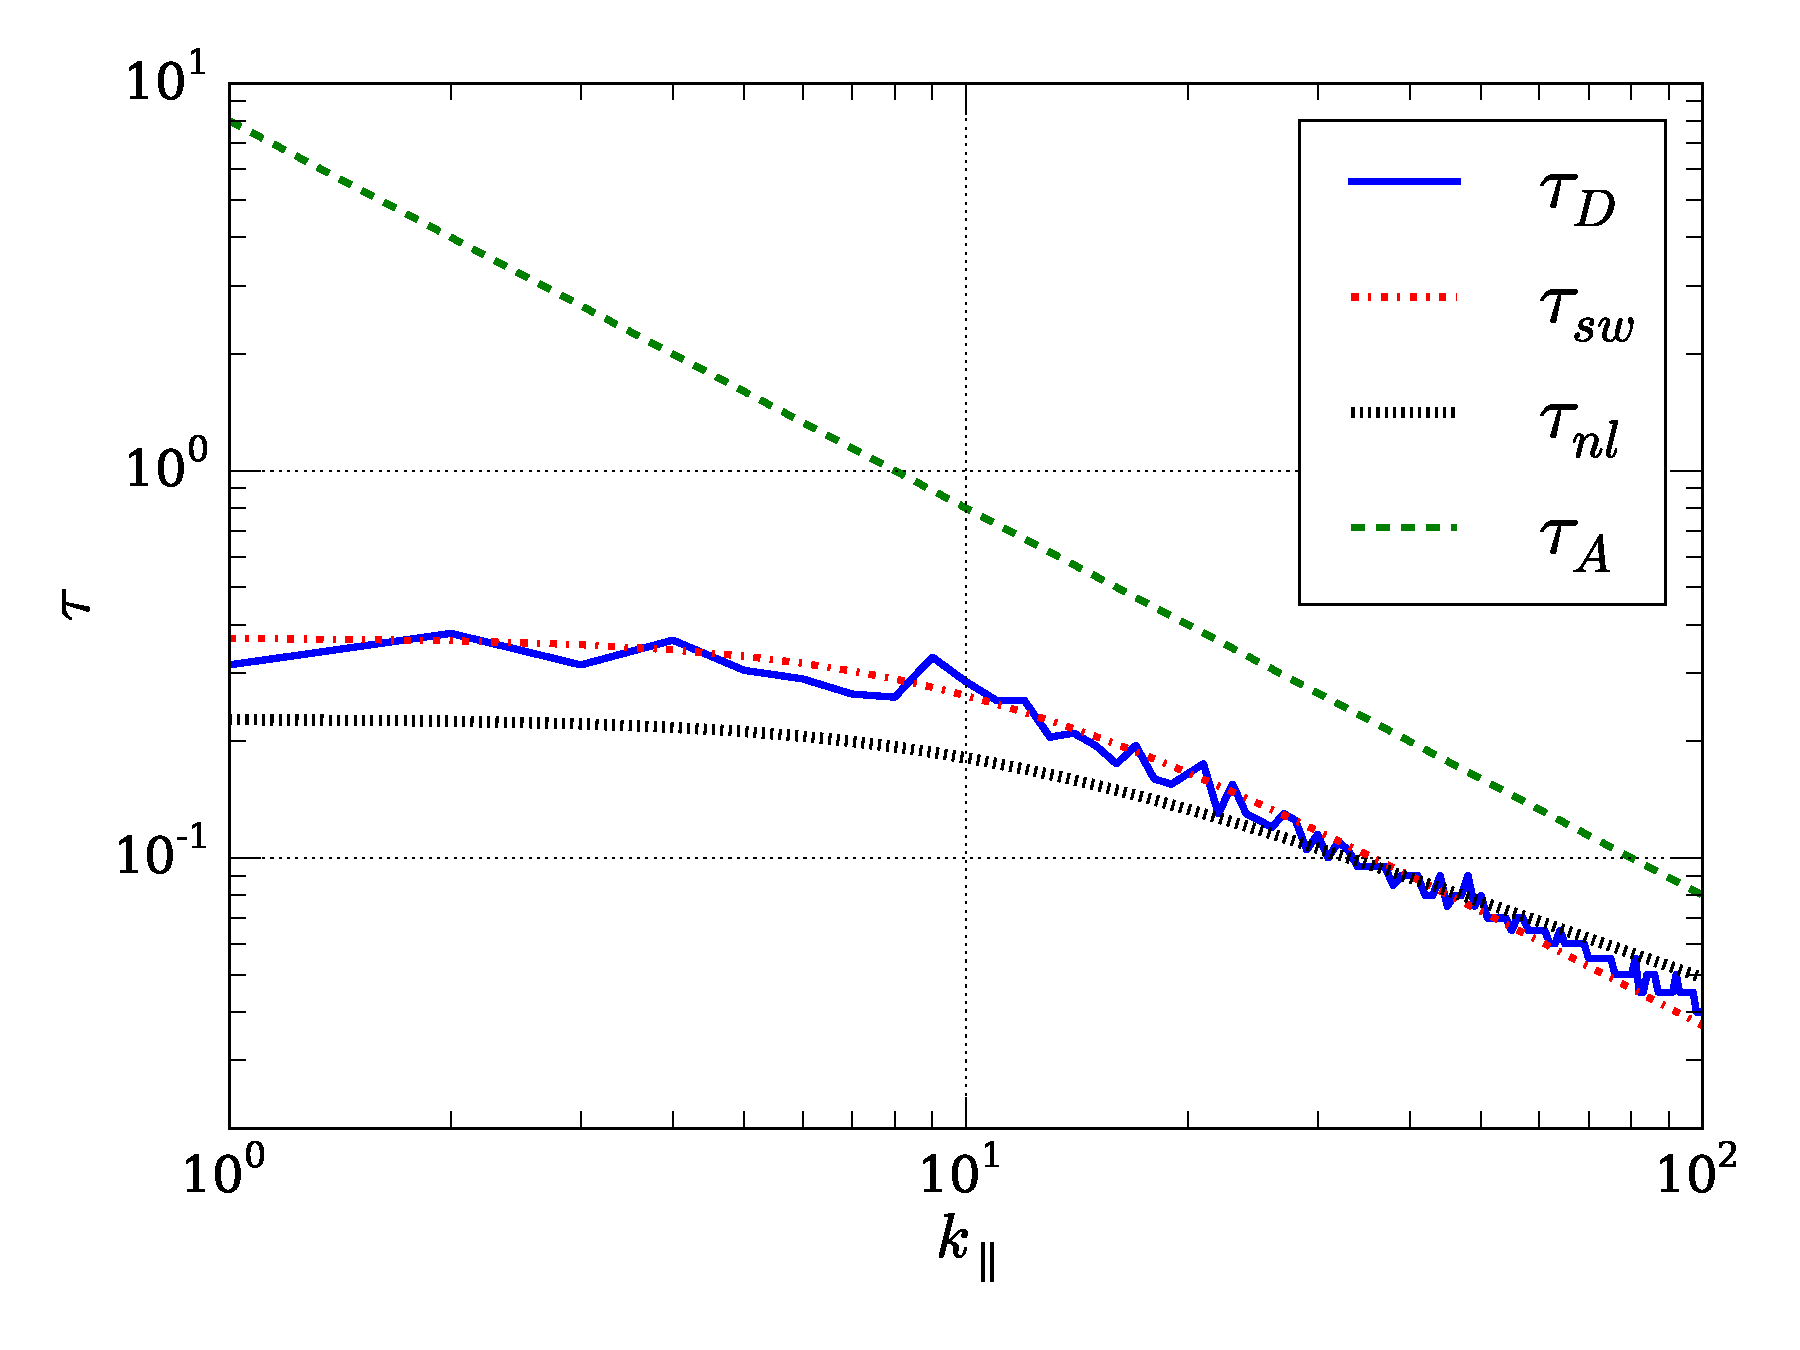
\includegraphics[width=0.49\columnwidth]{SpatioTemporalSpectra/fig5_B025_b_kperp_10-eps-converted-to.pdf}}

  \subfigure[$k_\perp=20$]{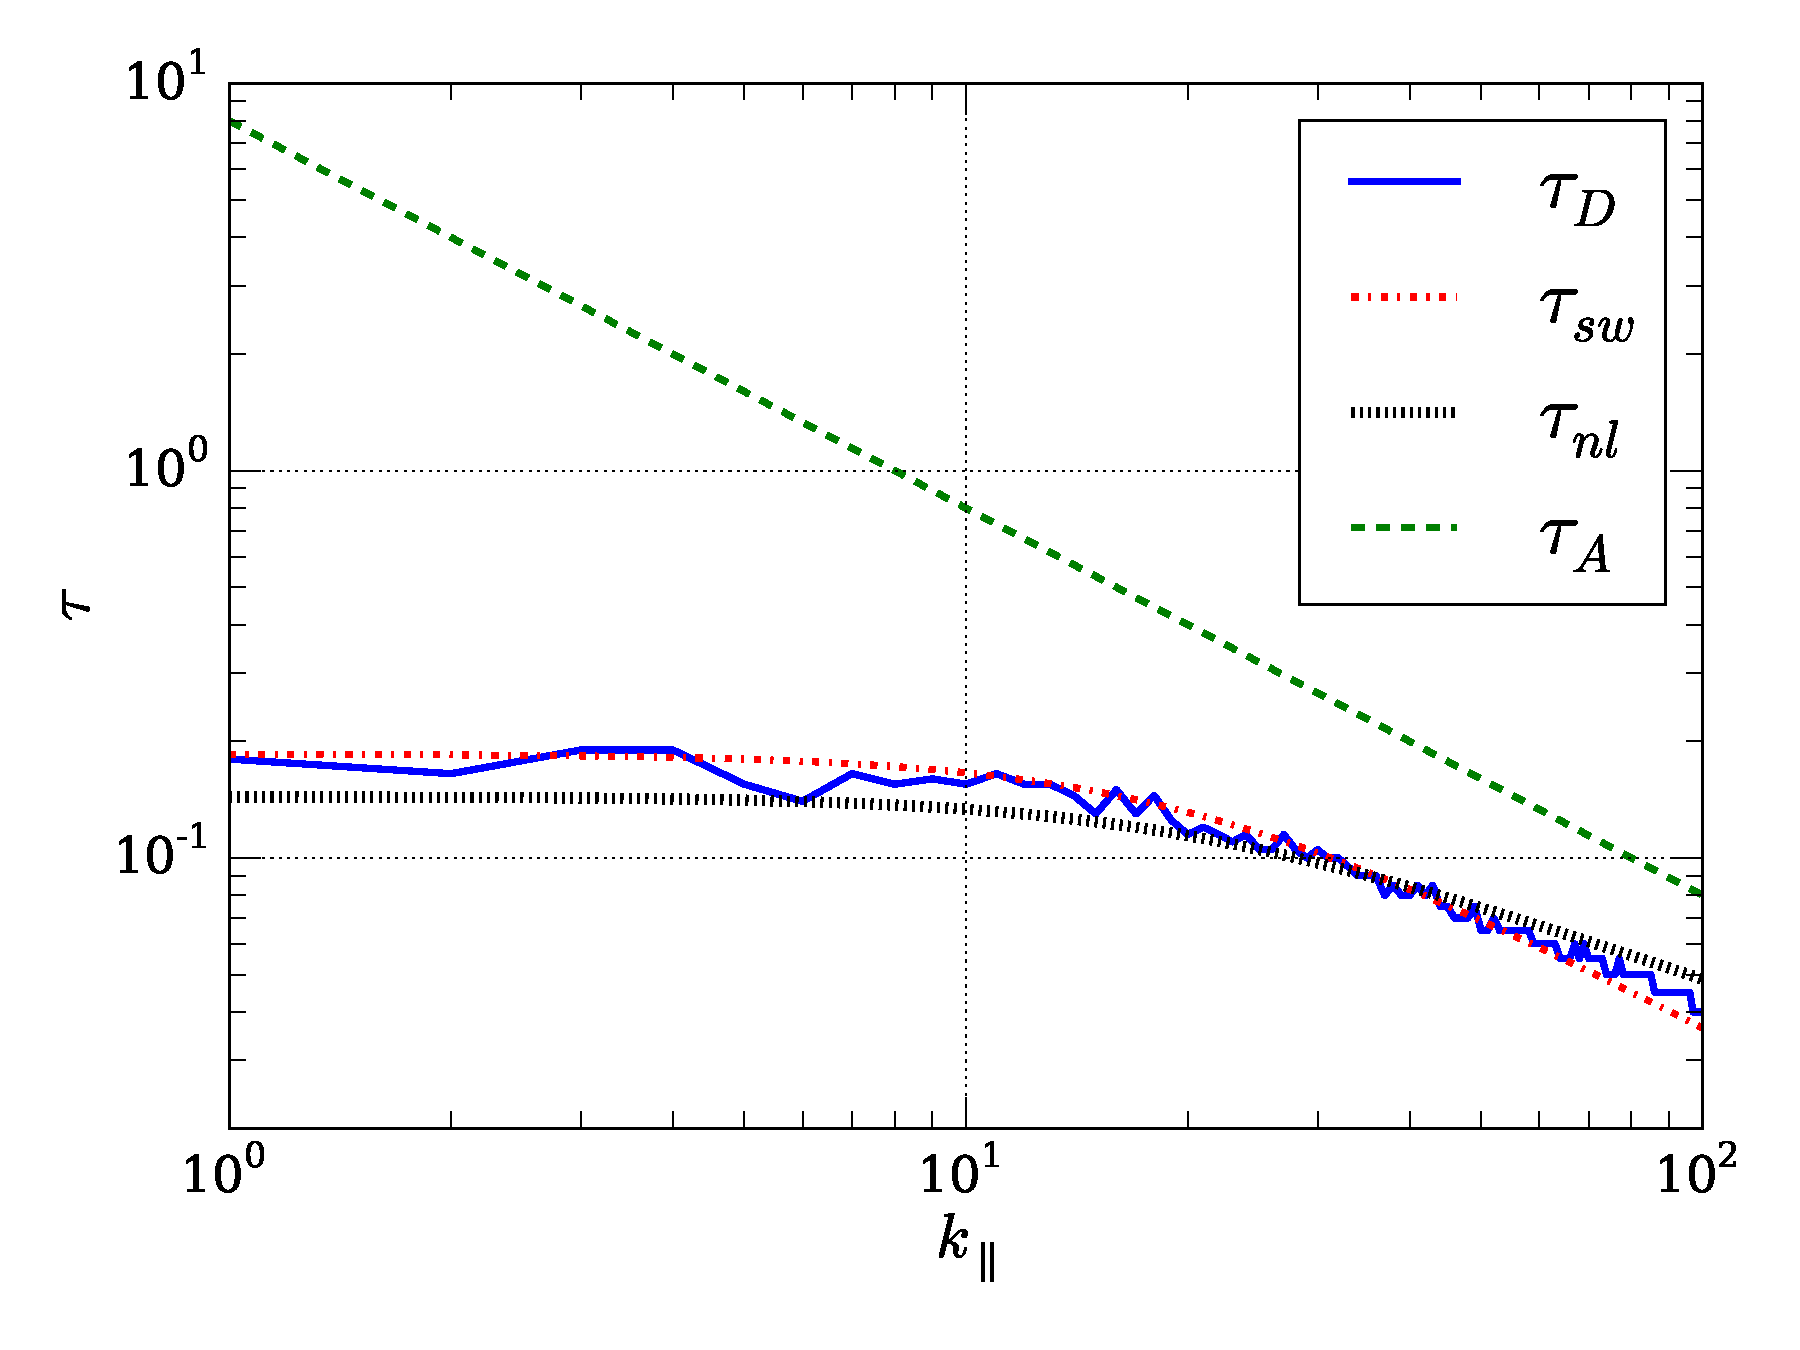
\includegraphics[width=0.49\columnwidth]{SpatioTemporalSpectra/fig5_B025_b_kperp_20-eps-converted-to.pdf}}
  \caption{Tiempo de descorrelación $\tau_D$ para la simulación con
    $B_0=0.25$. En cada panel, $k_\perp$ se mantiene constante y
    $k_\parallel$ se varía: (a) $k_\perp = 0$, (b) $k_\perp = 10$,
    y (c) $k_\perp = 20$. Las curvas indican las predicciones teóricas
    para varias escalas temporales físicas relevantes. El valor medido de $\tau_D$
    se encuentra siempre cerca de $\tau_{sw}$, excepto para $k_\perp = 0$
    y $k_\parallel$ entre $1$ y $5$, en donde la escala temporal
    dominante es el tiempo de Alfv\'en.}
  \label{fig3-5:B025_bvf_b_kperp}
\end{figure}

\begin{figure}
  \centering
  \subfigure[$k_\parallel=0$]{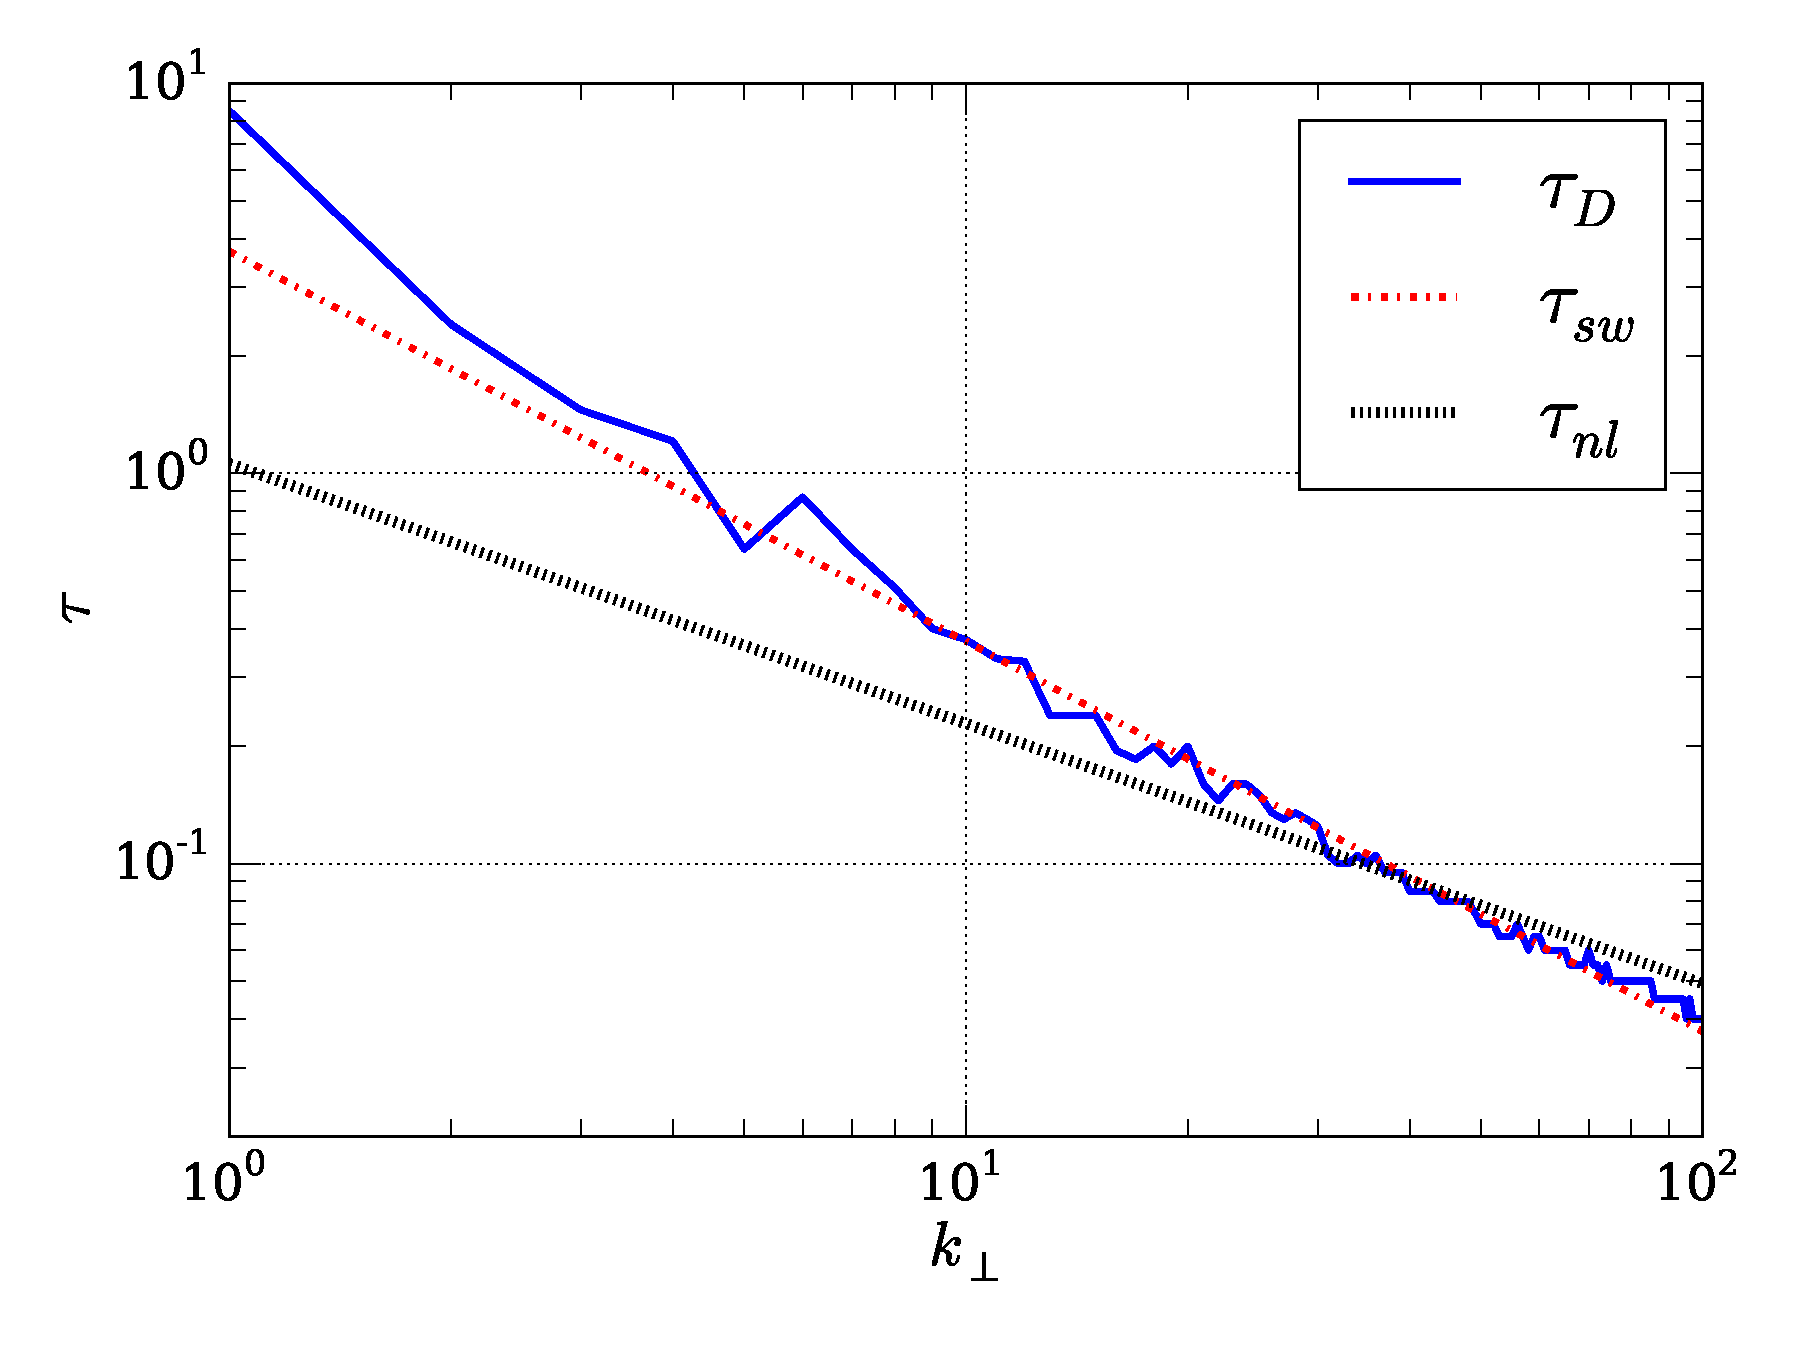
\includegraphics[width=0.49\columnwidth]{SpatioTemporalSpectra/fig5_B025_b_kpara_0-eps-converted-to.pdf}}
  \subfigure[$k_\parallel=10$]{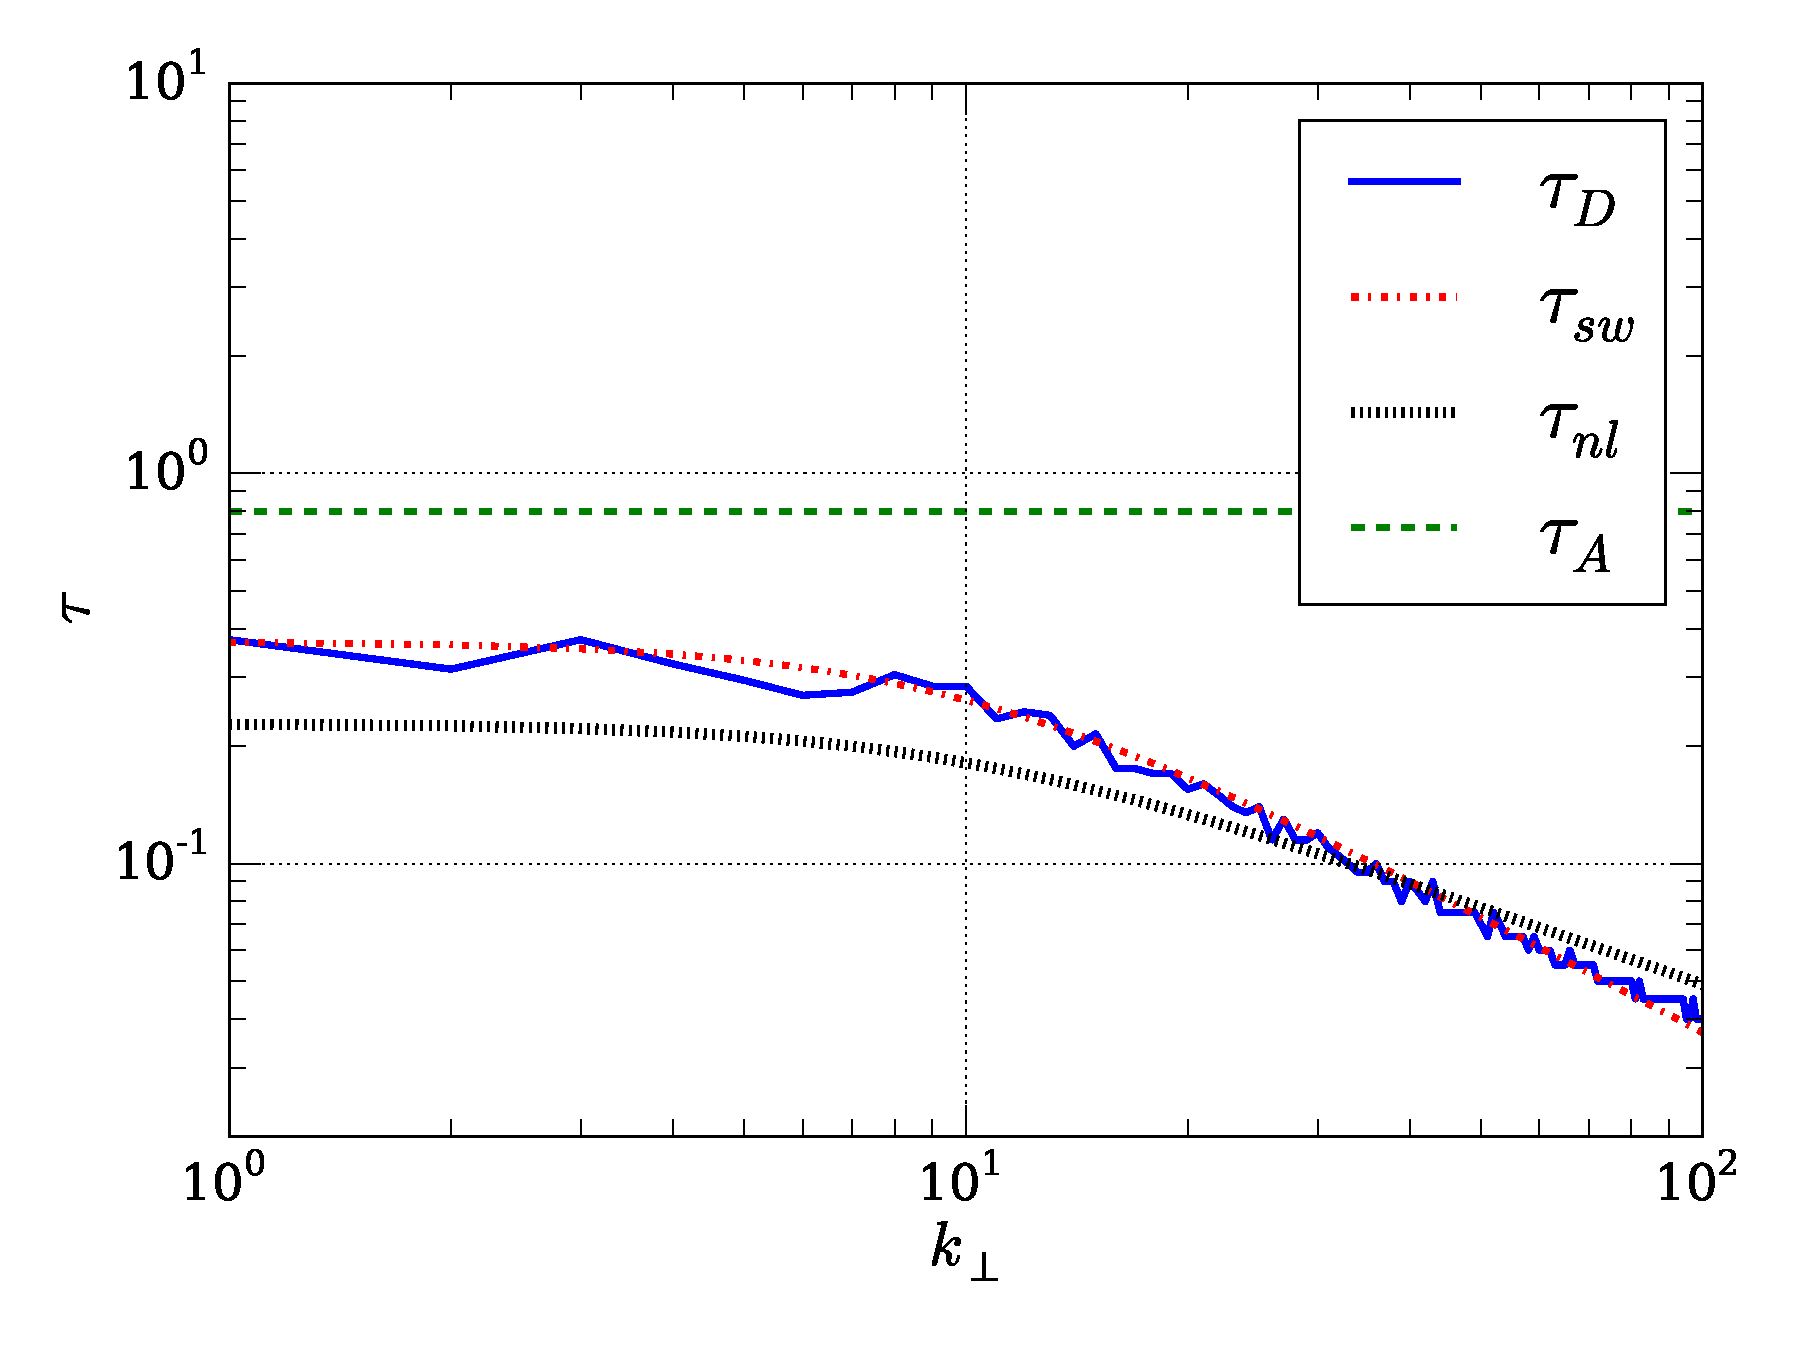
\includegraphics[width=0.49\columnwidth]{SpatioTemporalSpectra/fig5_B025_b_kpara_10-eps-converted-to.pdf}}

  \subfigure[$k_\parallel=20$]{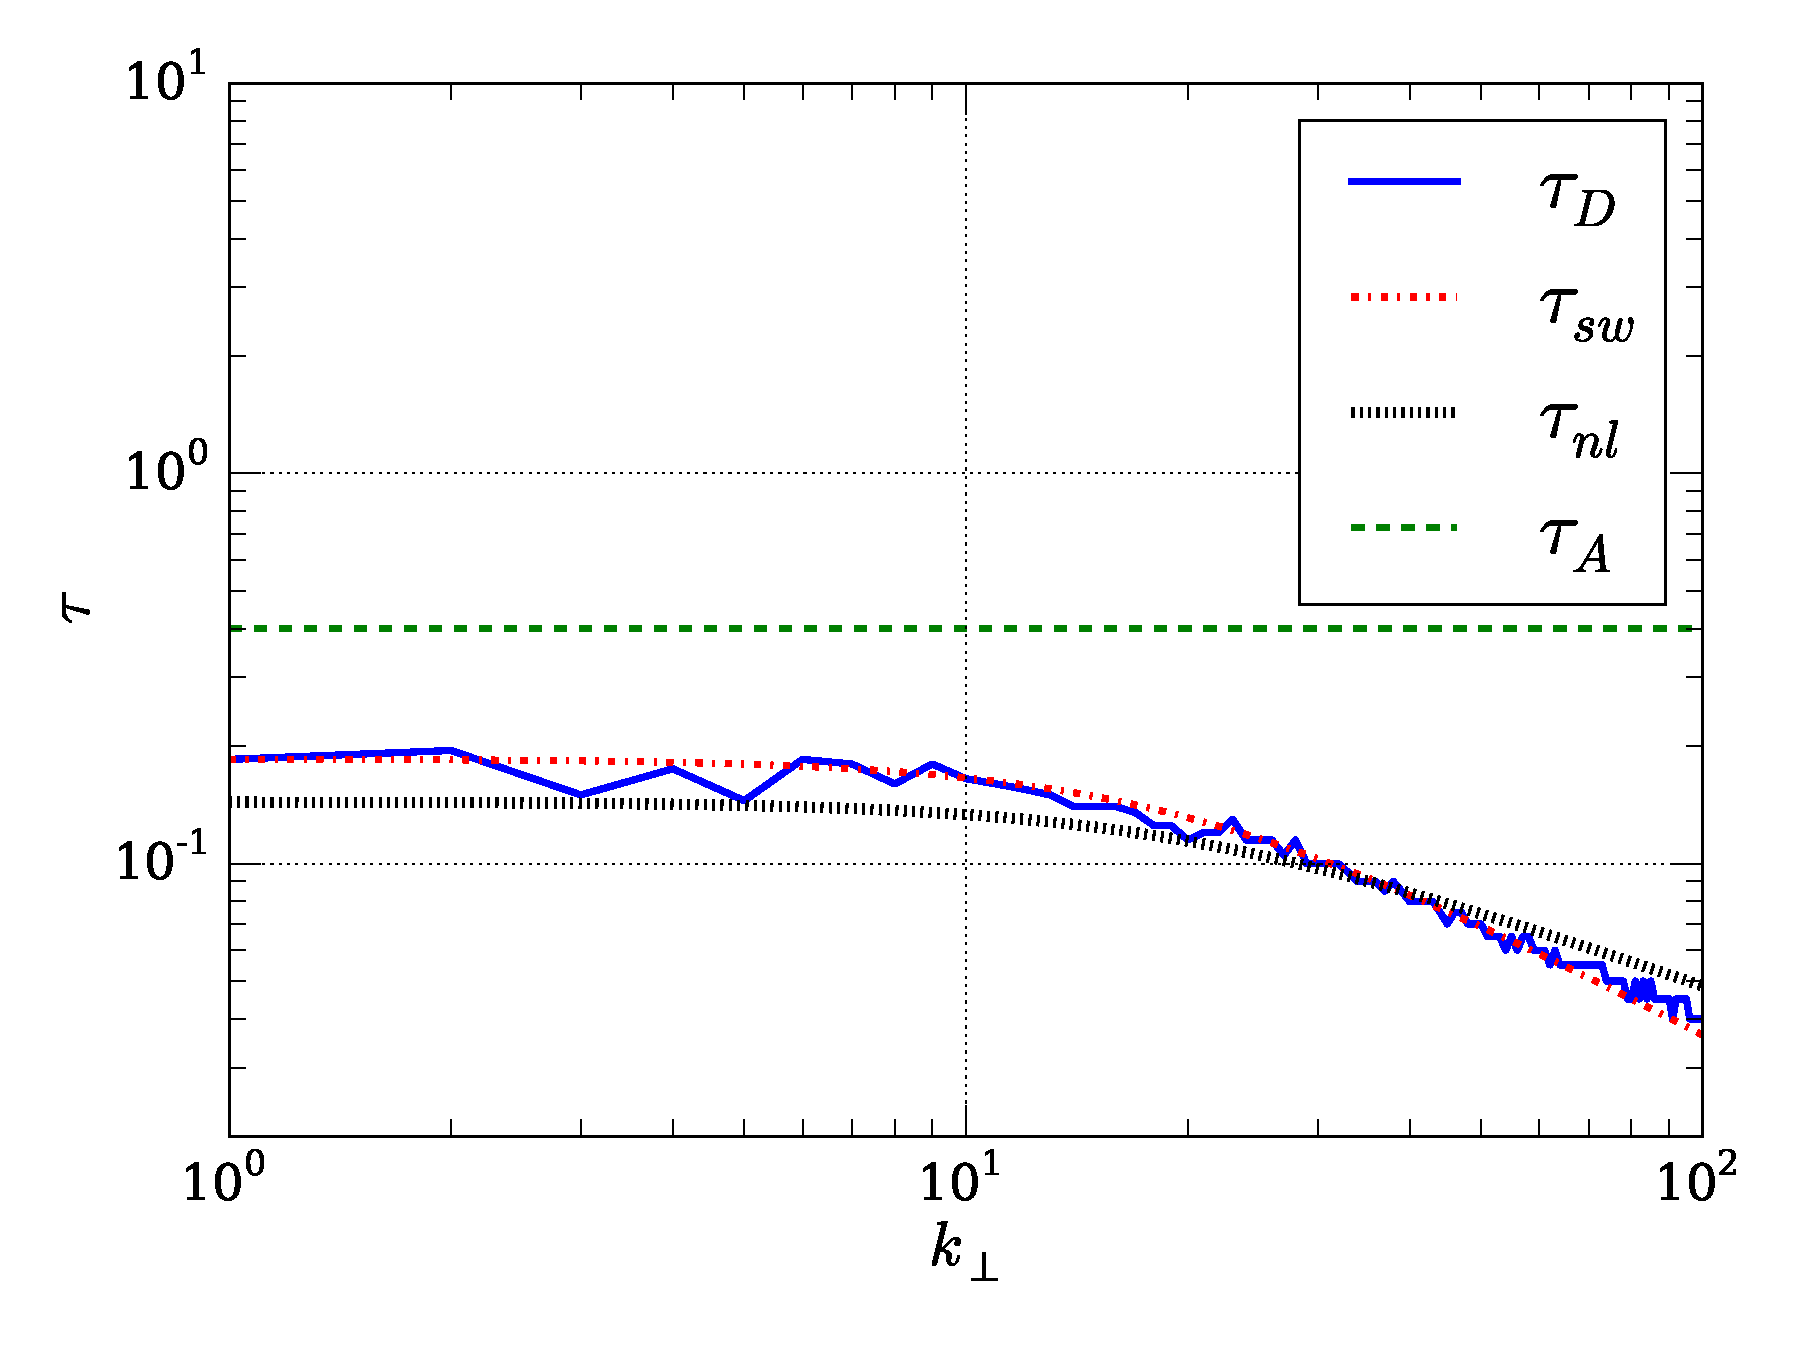
\includegraphics[width=0.49\columnwidth]{SpatioTemporalSpectra/fig5_B025_b_kpara_20-eps-converted-to.pdf}}
  \caption{Tiempo de descorrelación $\tau_D$ para la simulación con
    $B_0=0.25$. En cada panel, $k_\parallel$ se mantiene constante y
    $k_\perp$ se varía: (a) $k_\parallel = 0$, (b) $k_\parallel = 10$,
    y (c) $k_\parallel = 20$. Las curvas indican las predicciones teóricas
    para varias escalas temporales físicas relevantes. El valor medido de $\tau_D$
    se encuentra siempre cerca de $\tau_{sw}$.}
  \label{fig3-5:B025_bvf_b_kpara}
\end{figure}

\begin{figure}
  \centering
  \subfigure[$k_\perp=0$]{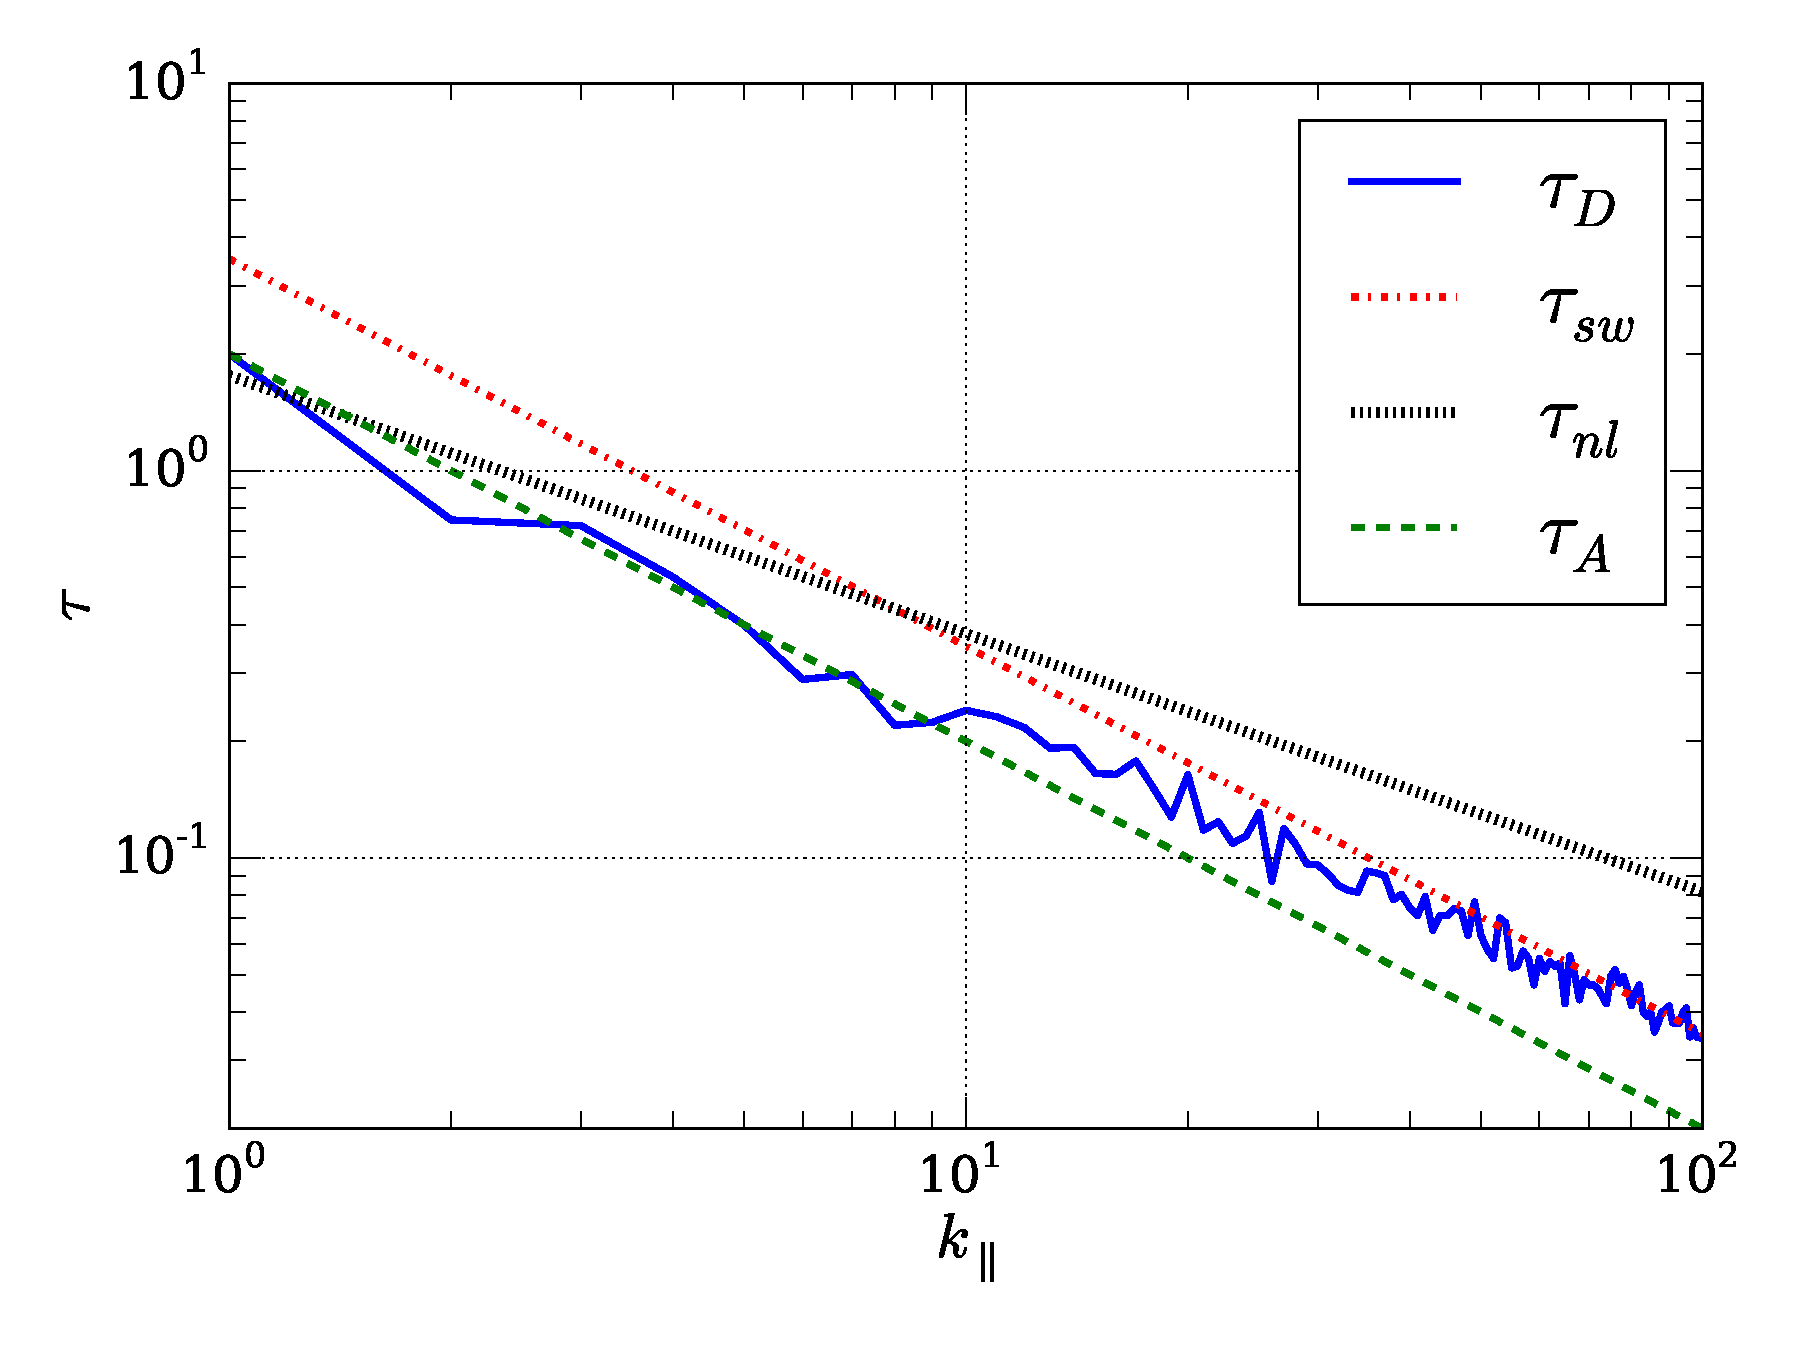
\includegraphics[width=0.49\columnwidth]{SpatioTemporalSpectra/fig5_B1_b_kperp_0-eps-converted-to.pdf}}
  \subfigure[$k_\perp=10$]{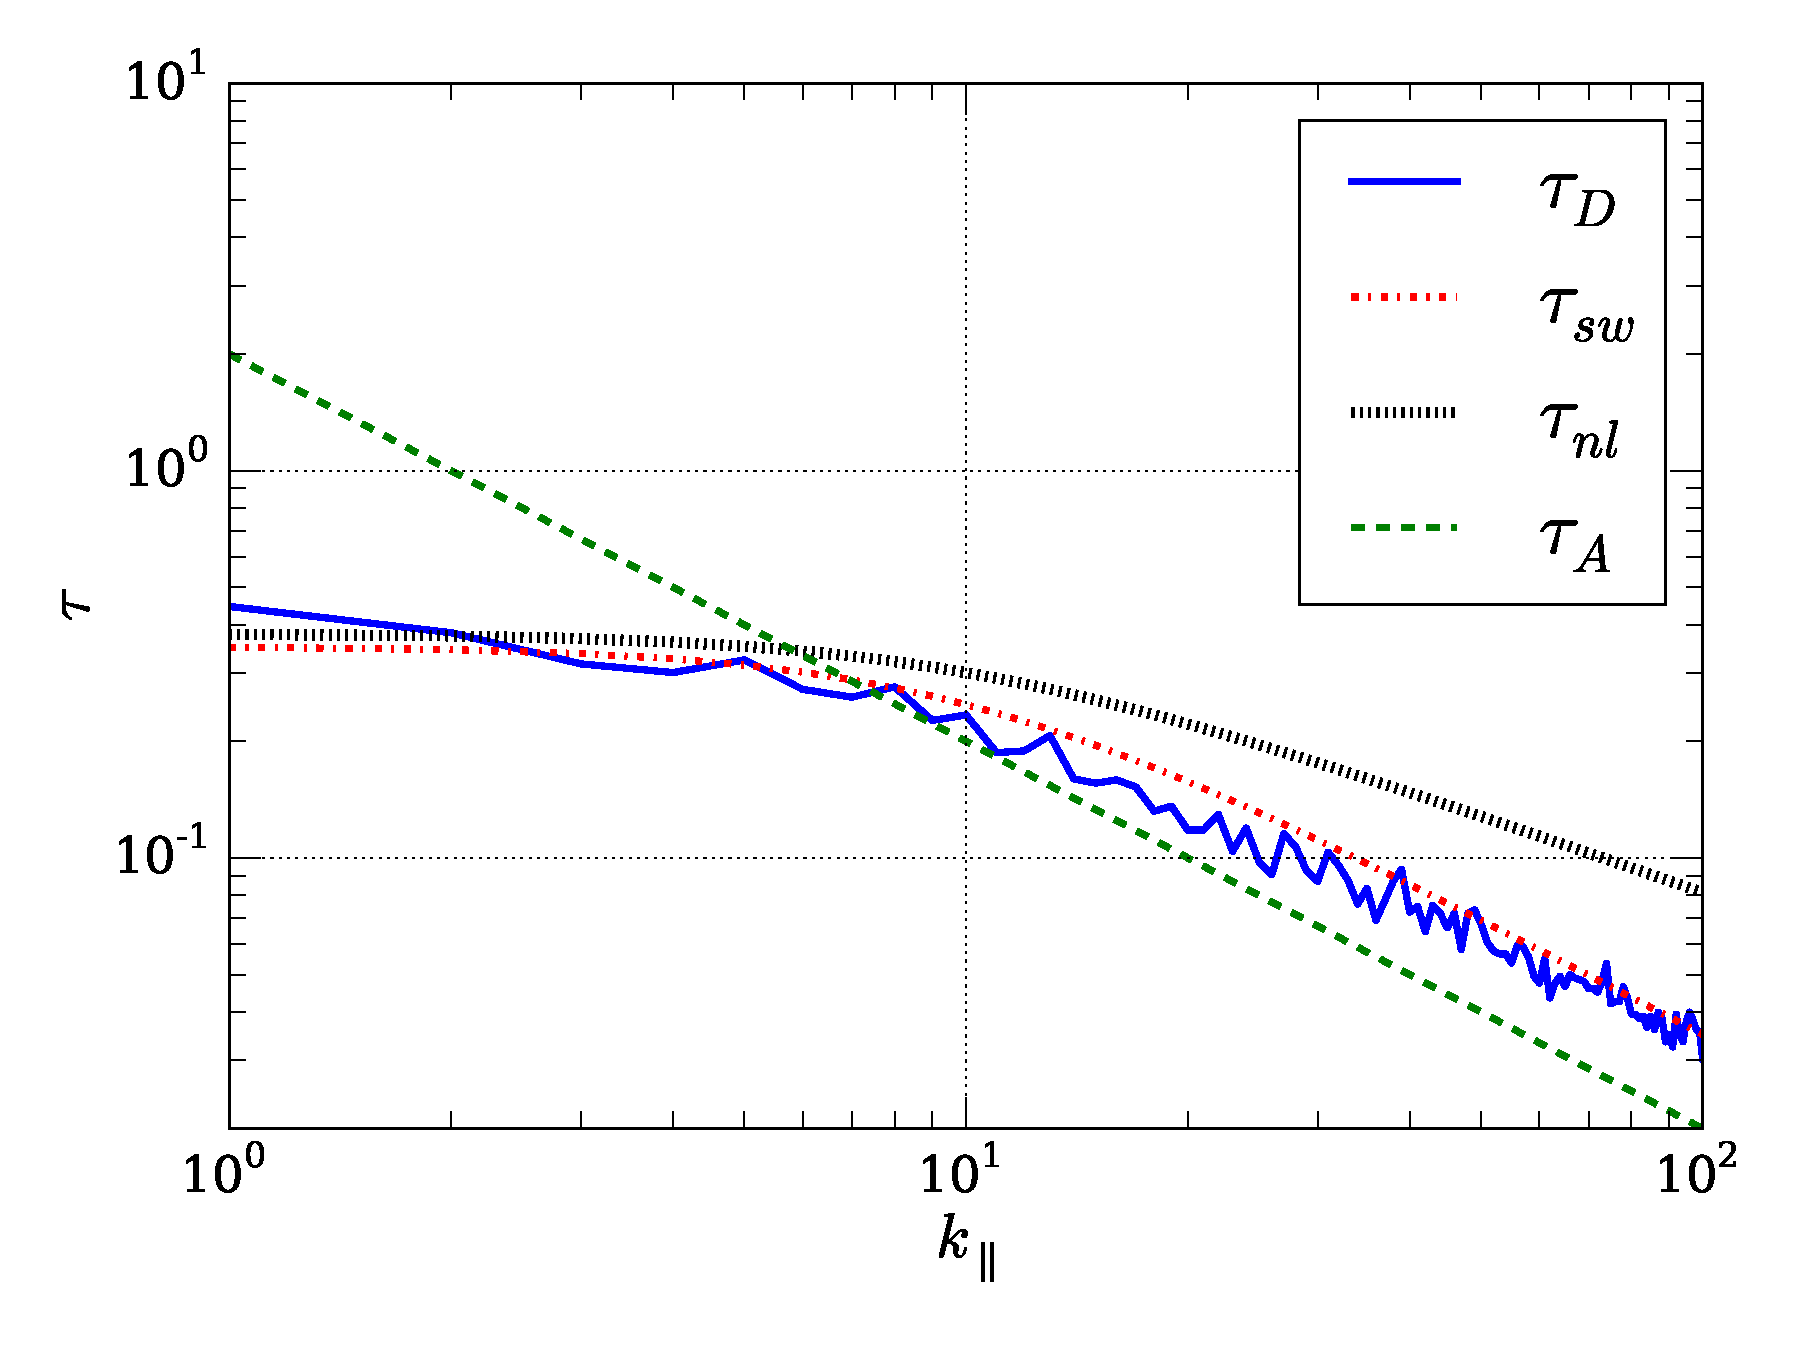
\includegraphics[width=0.49\columnwidth]{SpatioTemporalSpectra/fig5_B1_b_kperp_10-eps-converted-to.pdf}}

  \subfigure[$k_\perp=20$]{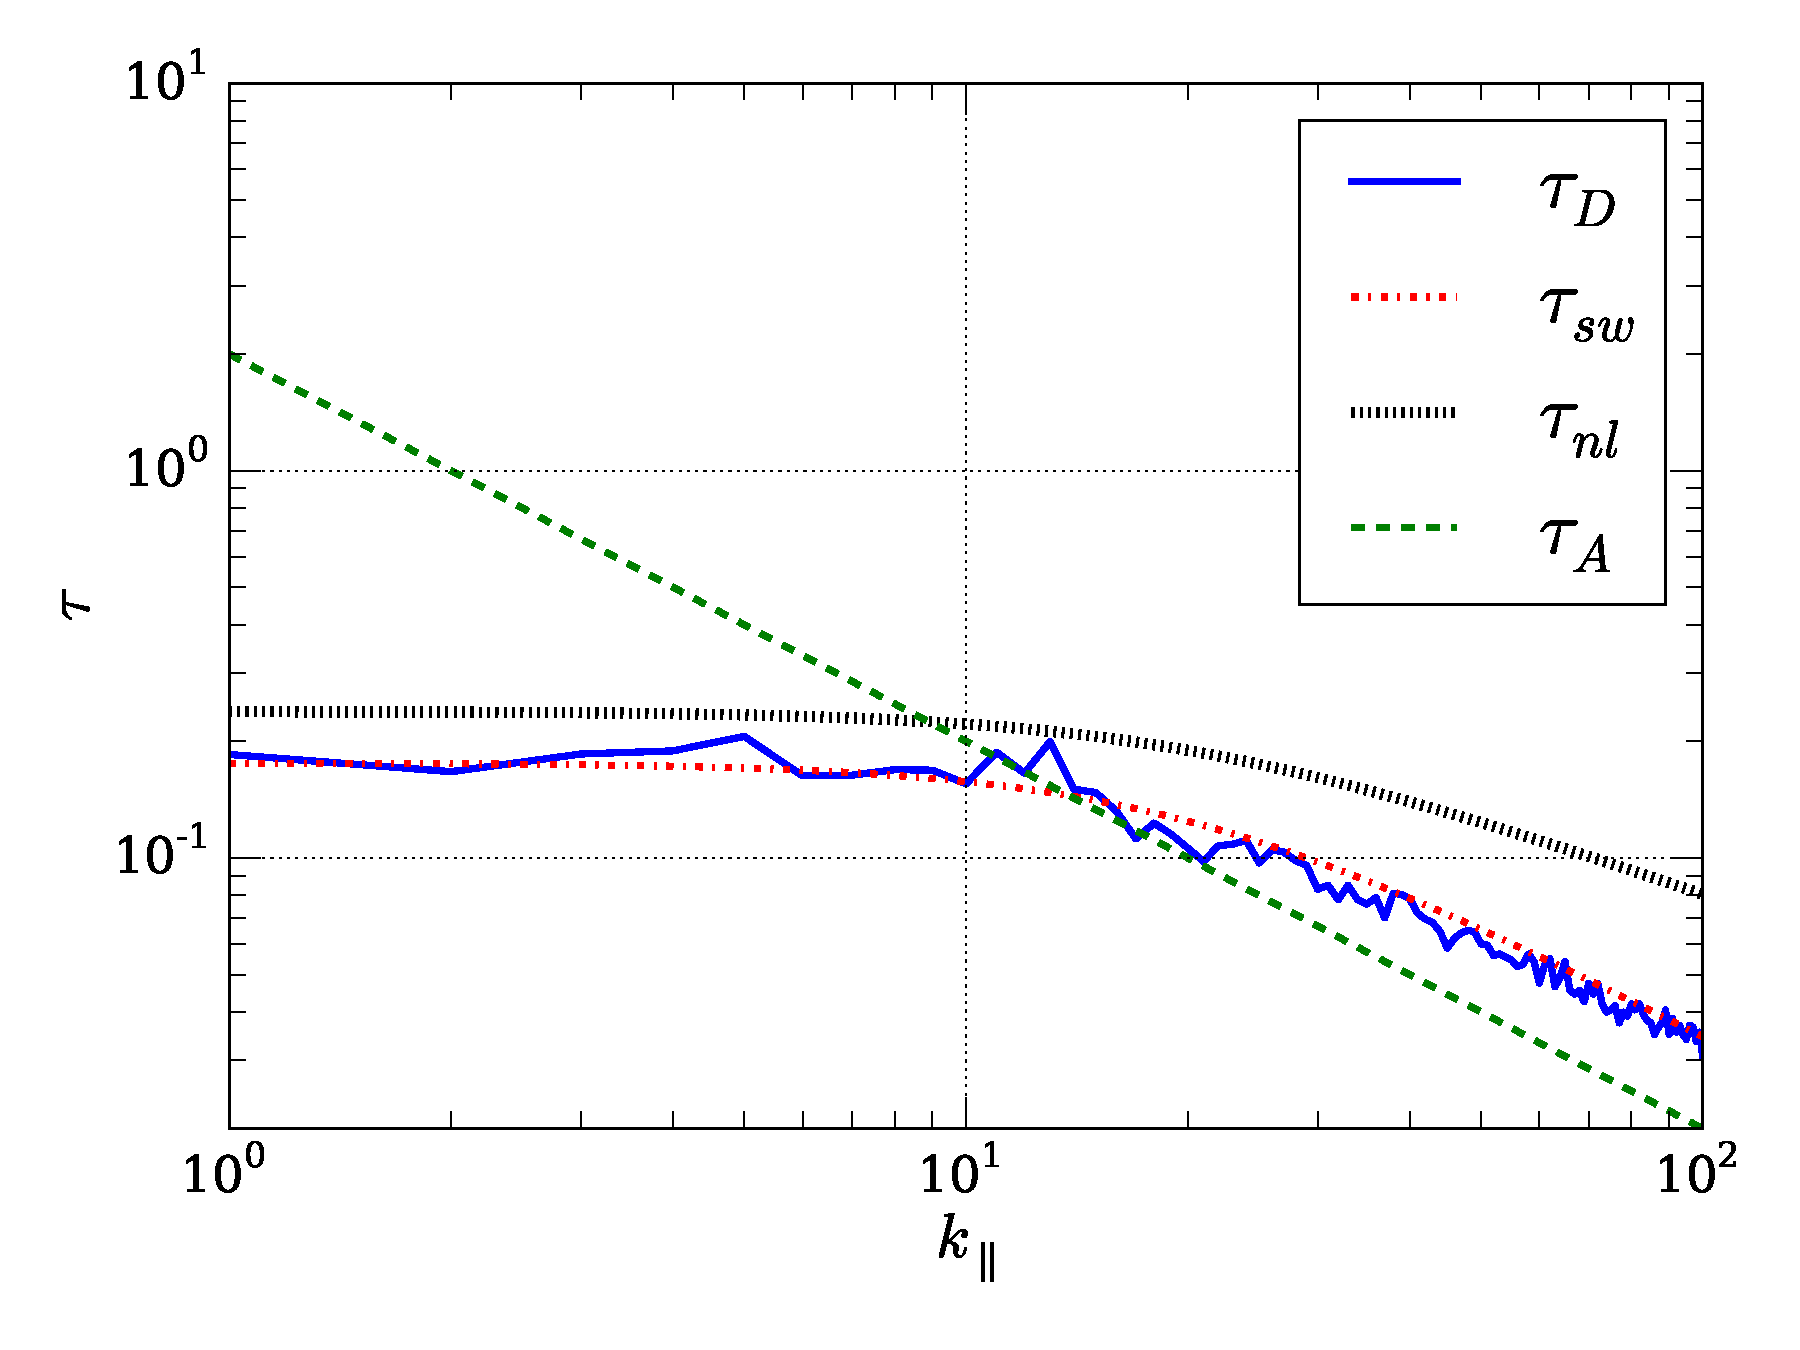
\includegraphics[width=0.49\columnwidth]{SpatioTemporalSpectra/fig5_B1_b_kperp_20-eps-converted-to.pdf}}
  \caption{Tiempo de descorrelación $\tau_D$ para la simulación con
    $B_0=1$. En cada panel, $k_\perp$ se mantiene constante y
    $k_\parallel$ se varía: (a) $k_\perp = 0$, (b) $k_\perp = 10$,
    y (c) $k_\perp = 20$. Las curvas indican las predicciones teóricas
    para varias escalas temporales físicas relevantes.}
  \label{fig3-5:B1_bvf_b_kperp}
\end{figure}

\begin{figure}
  \centering
  \subfigure[$k_\parallel=0$]{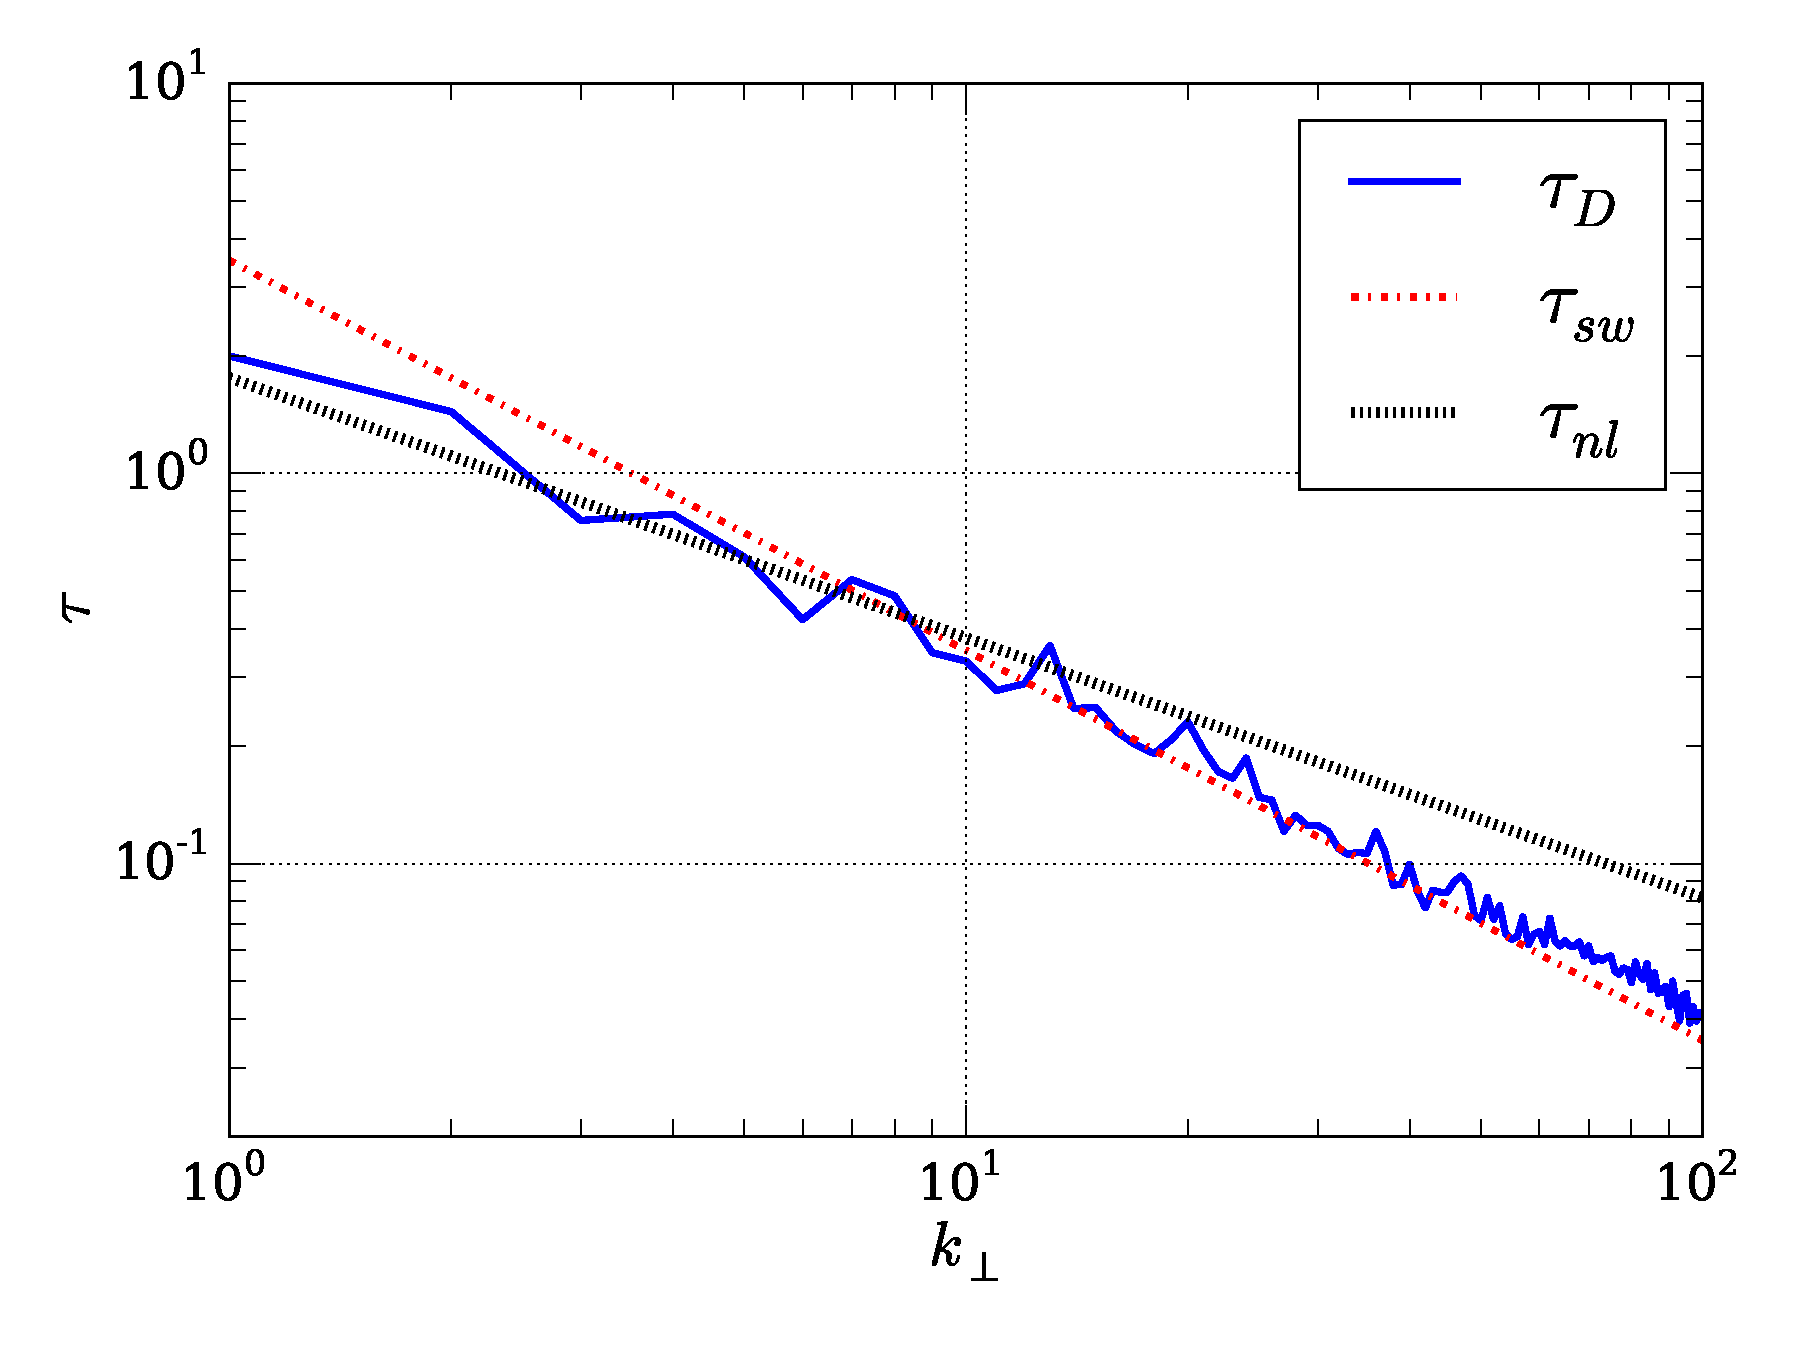
\includegraphics[width=0.49\columnwidth]{SpatioTemporalSpectra/fig5_B1_b_kpara_0-eps-converted-to.pdf}}
  \subfigure[$k_\parallel=10$]{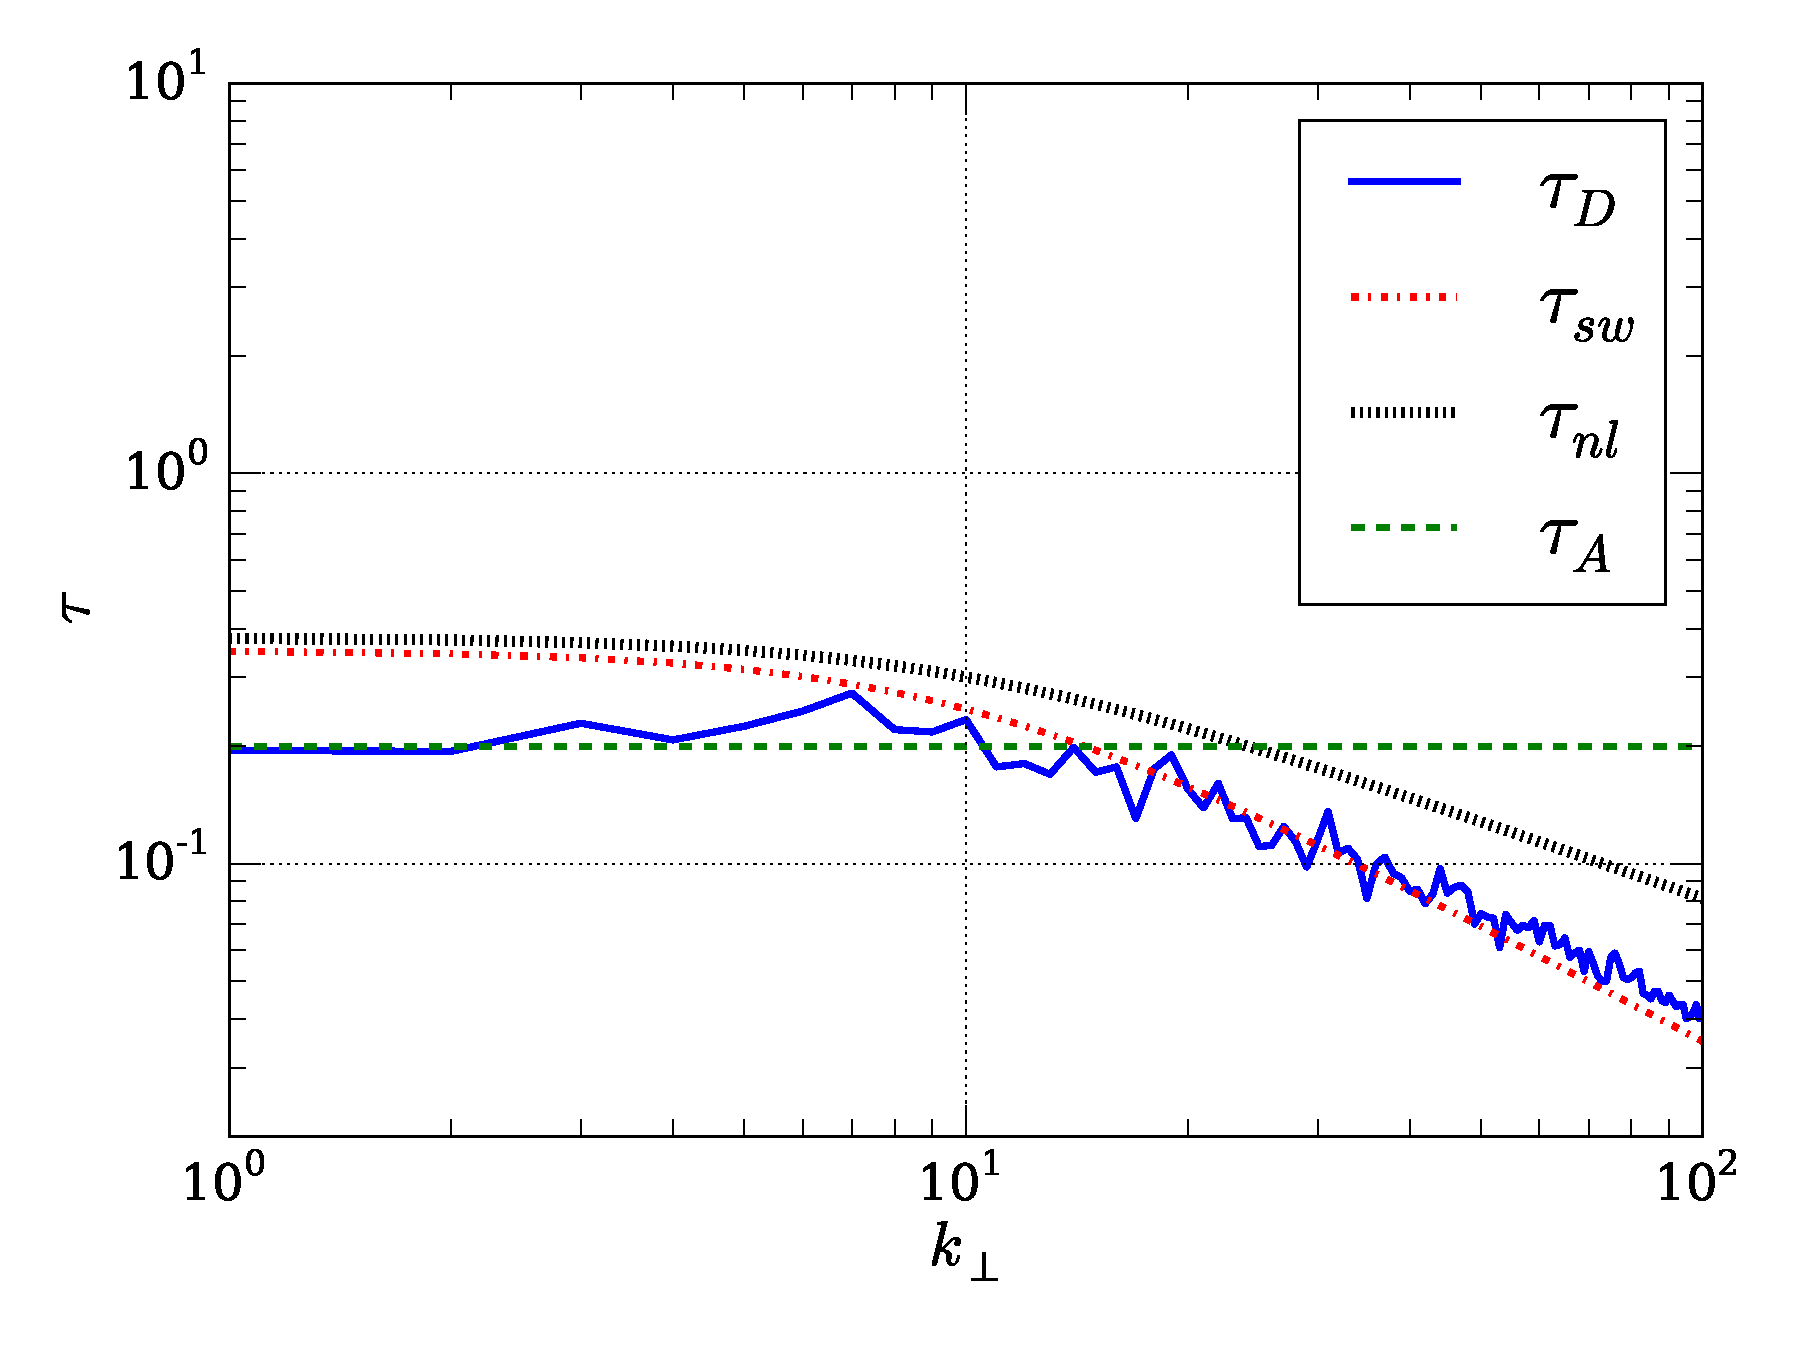
\includegraphics[width=0.49\columnwidth]{SpatioTemporalSpectra/fig5_B1_b_kpara_10-eps-converted-to.pdf}}

  \subfigure[$k_\parallel=20$]{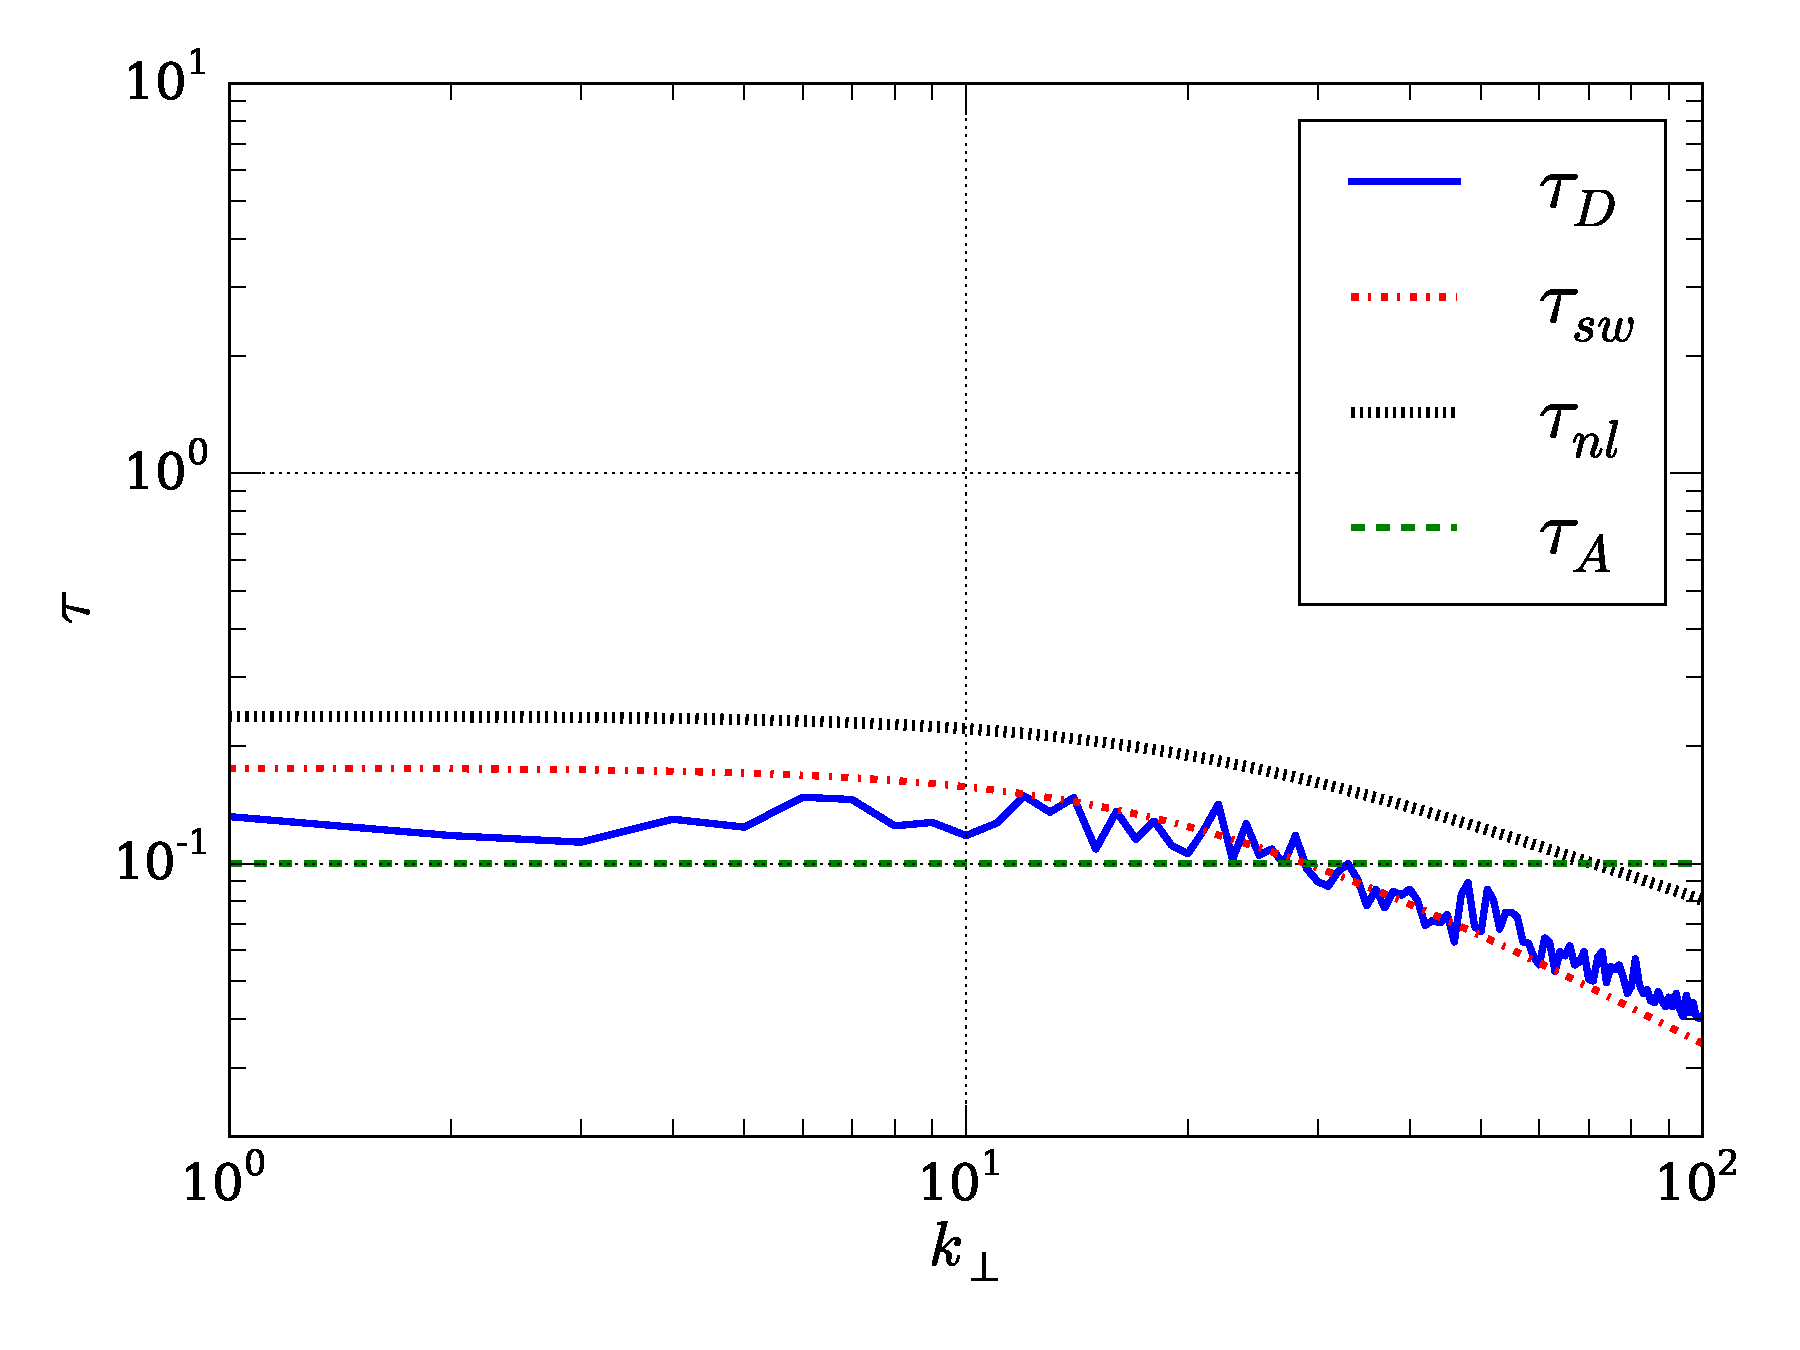
\includegraphics[width=0.49\columnwidth]{SpatioTemporalSpectra/fig5_B1_b_kpara_20-eps-converted-to.pdf}}
  \caption{Tiempo de descorrelación $\tau_D$ para la simulación con
    $B_0=1$. En cada panel, $k_\parallel$ se mantiene constante y
    $k_\perp$ se varía: (a) $k_\parallel = 0$, (b) $k_\parallel = 10$,
    y (c) $k_\parallel = 20$. Las curvas indican las predicciones teóricas
    para varias escalas temporales físicas relevantes.}
  \label{fig3-5:B1_bvf_b_kpara}
\end{figure}

Finalmente, analicemos el comportamiento del tiempo de descorrelación
$\tau$ para las corridas con el mayor campo magnético medio
considerado, $B_0=8$. Los resultados se pueden ver en las
\cref{fig3-5:B8_bvf_b_kperp,fig3-5:B8_bvf_b_kpara}. Para valores pequeños
de $k_\perp$, se encuentra que el tiempo de Alfvén resulta dominante
de las descorrelaciones (hasta, aproximadamente, $k_\parallel = 10$;
ver \cref{fig3-5:B8_bvf_b_kpara}). Sin embargo, para valores mayores
de $k_{\perp}$, el tiempo de descorrelación se aleja del tiempo de
Alfvén y se acerca lentamente a la escala del tiempo
de \textit{sweeping}. Esto es consistente con los espectros
espacio-temporales de la
\cref{fig3-3:B8_bvf_Etot_kperp0}, donde se observa que la energía se
concentra cerca de la relación de dispersión de Alfvén para valores
pequeños del número de onda, pero se difumina hacia las frecuencias de
\textit{sweeping} para valores grandes del número de onda.  Como resultado, es
la competencia entre estas dos escalas temporales la que parece ser
responsable del ensanchamiento del espectro espacio-temporal para
valores grandes de $B_0$. En tanto el tiempo de Alfvén sea mucho más
rápido que las otras escalas temporales del sistema, el flujo excita
ondas de Alfvén, que dominan los modos de descorrelación. Pero cuando
las otras escalas se acercan a la escala temporal de las ondas (o
hasta se vuelven más rápidas, como sucede para valores pequeños de
$B_0$), el sistema cambia la escala temporal dominante en la
descorrelación.

\begin{figure}
  \centering
  \subfigure[$k_\perp=0$]{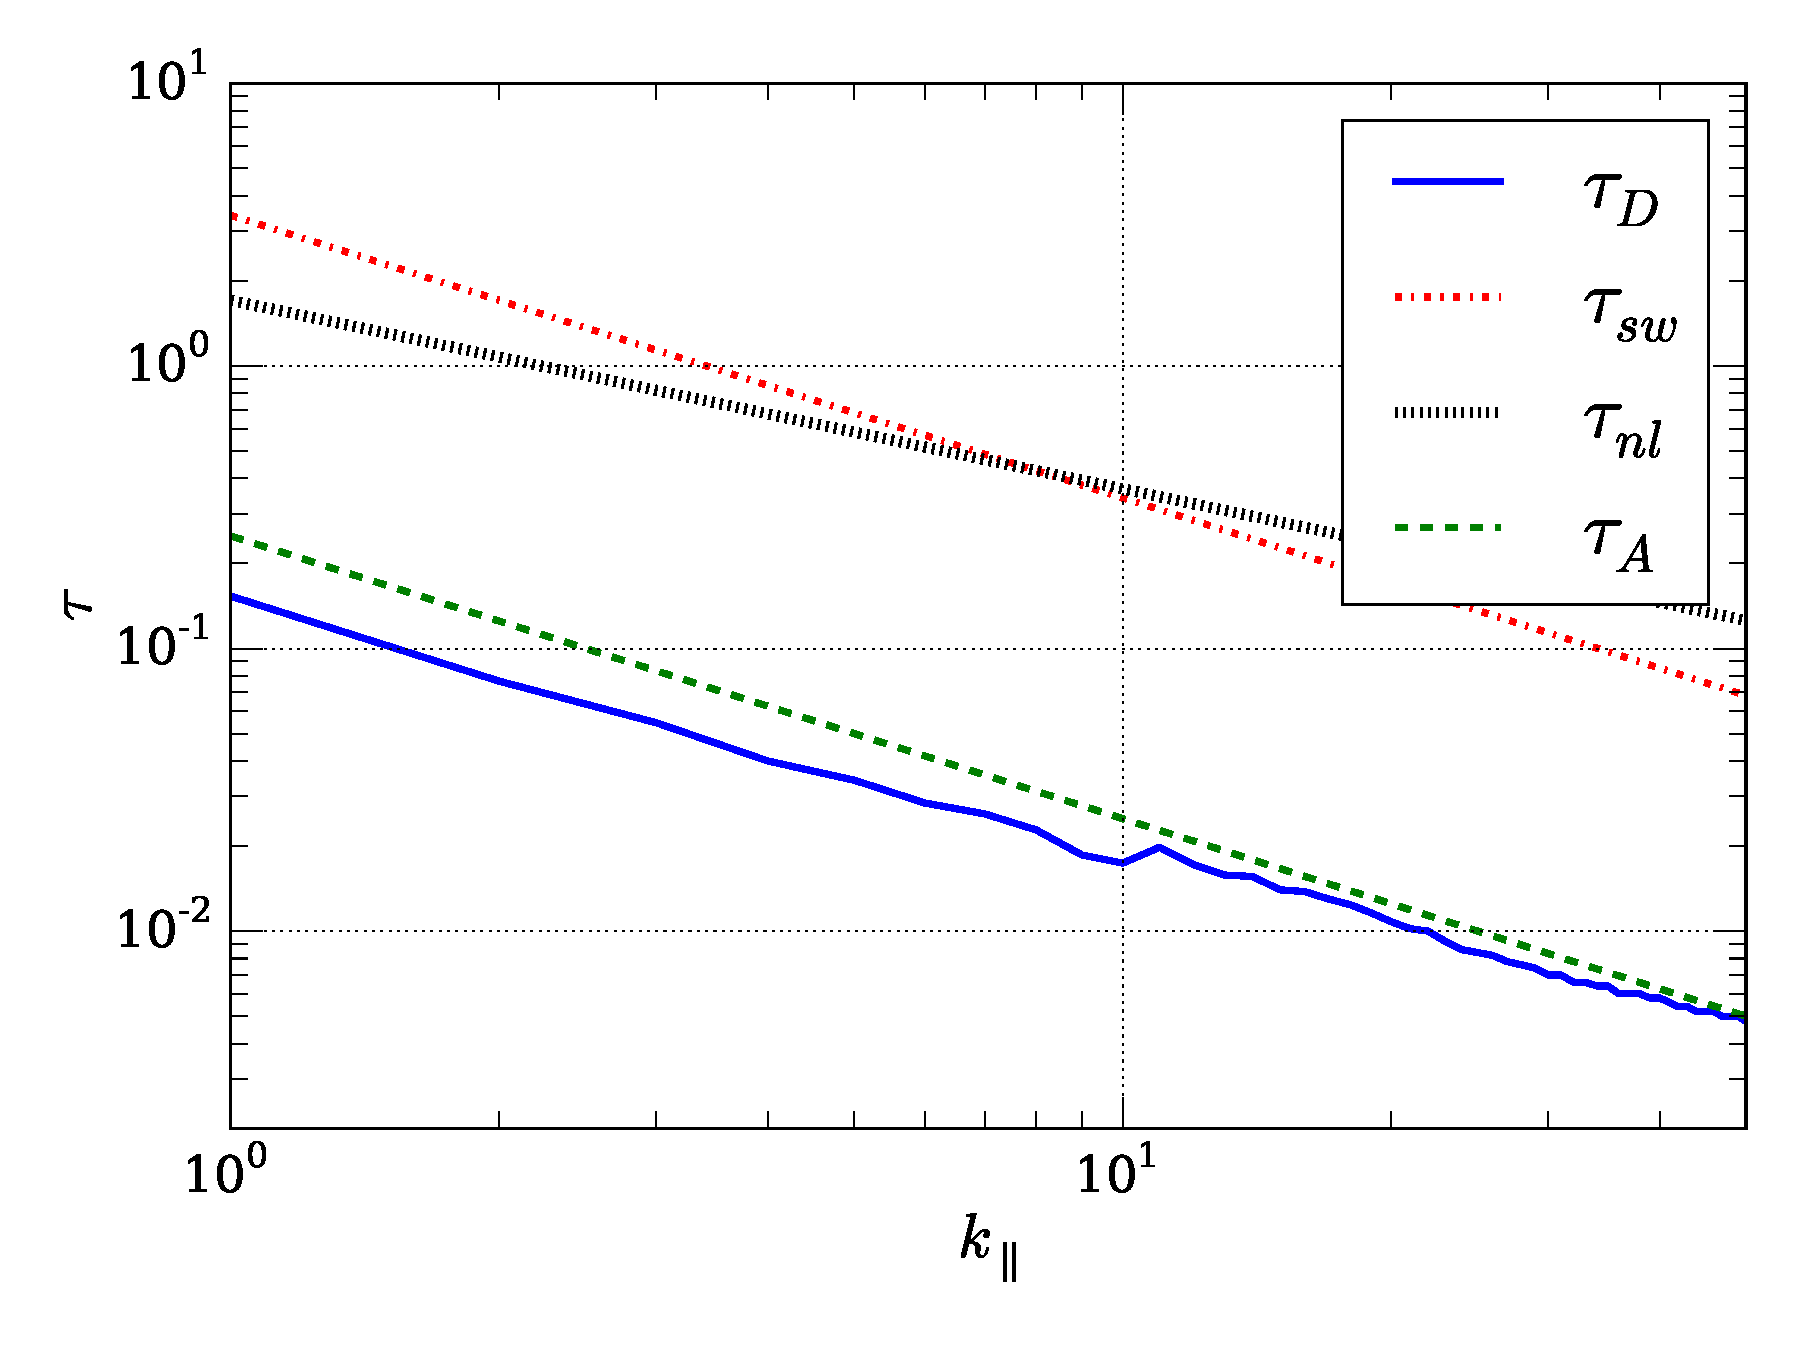
\includegraphics[width=0.49\columnwidth]{SpatioTemporalSpectra/fig5_B8_b_kperp_0-eps-converted-to.pdf}}
  \subfigure[$k_\perp=10$]{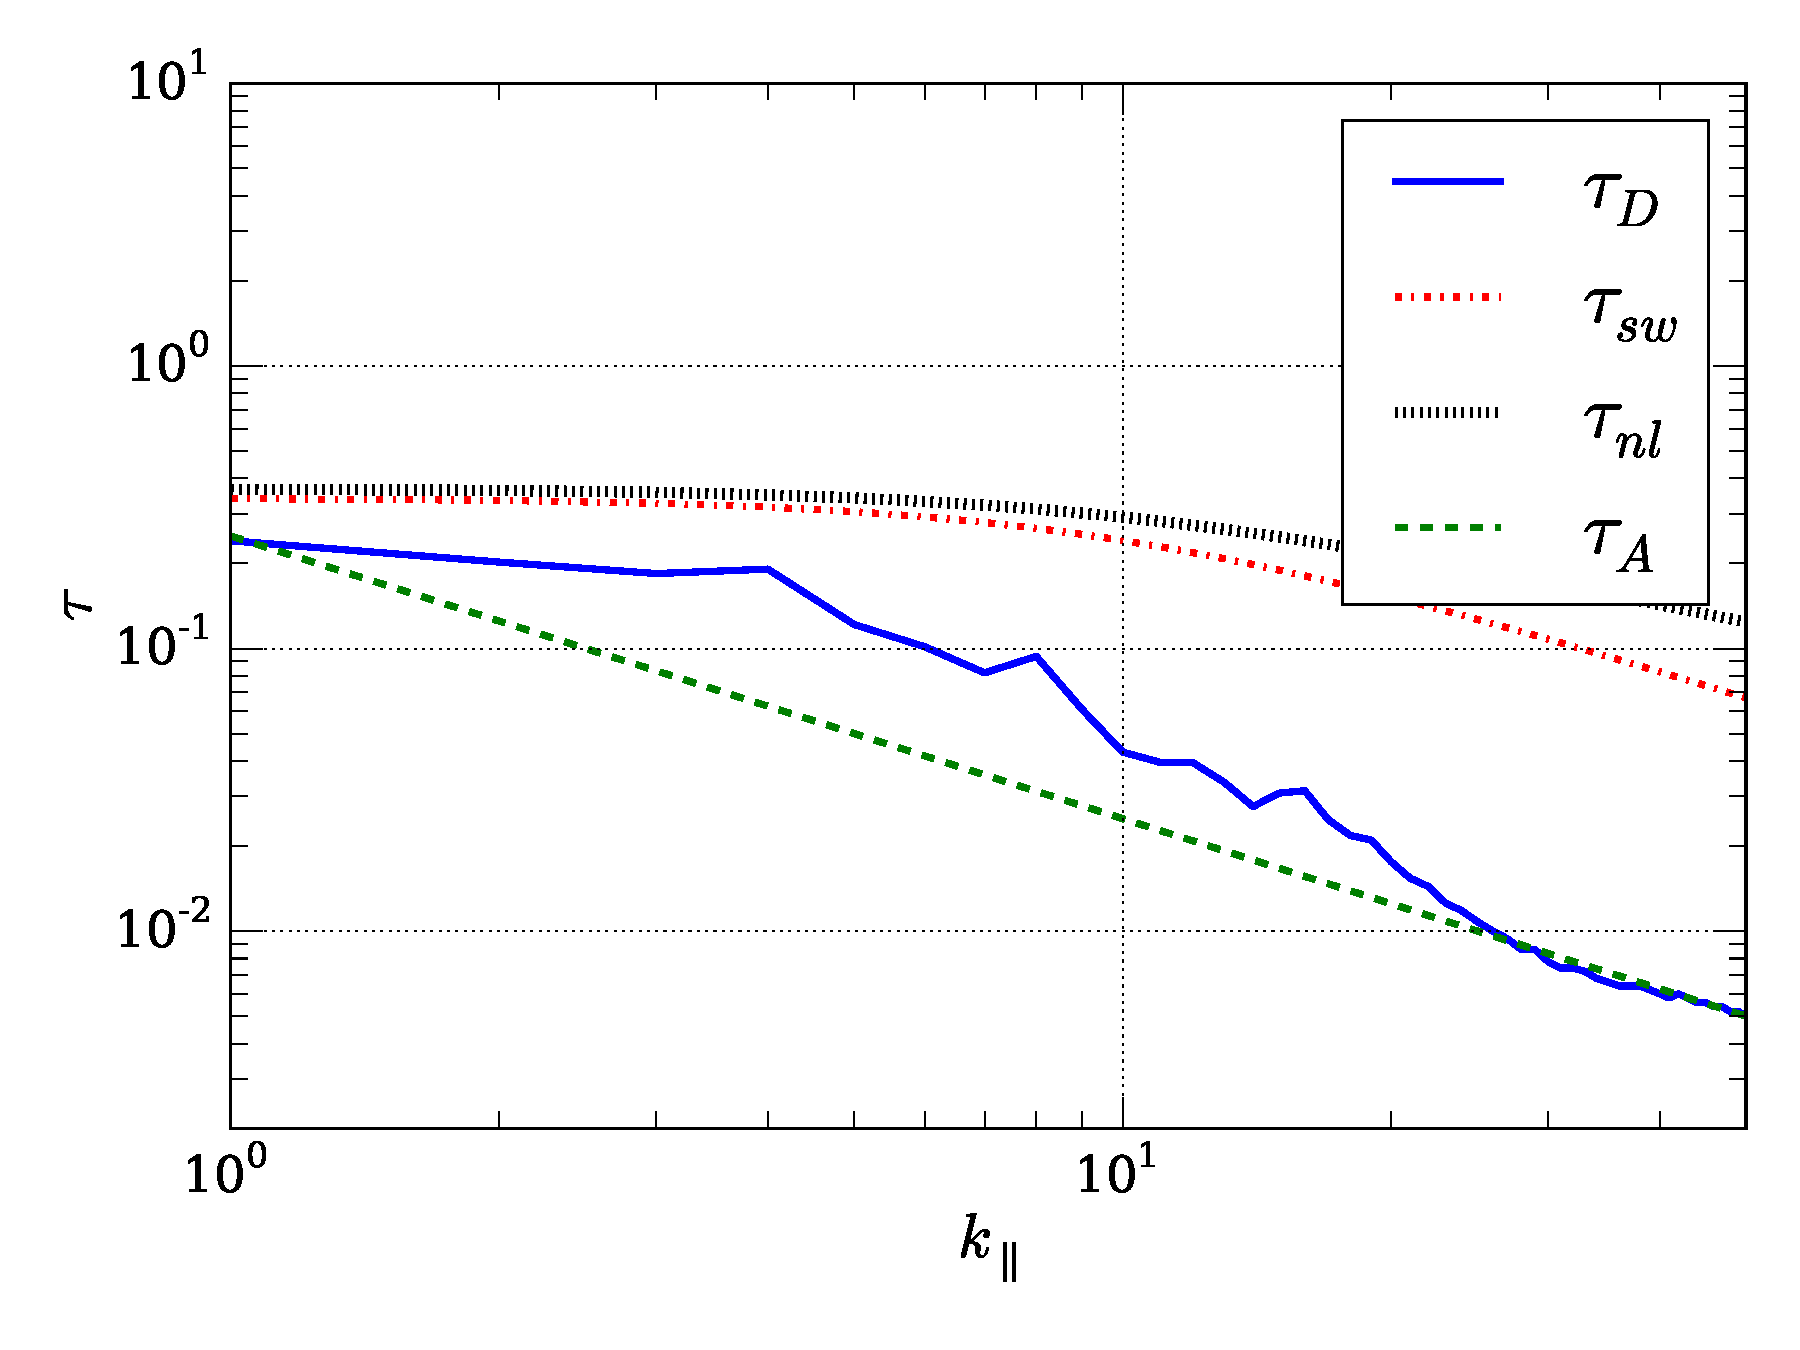
\includegraphics[width=0.49\columnwidth]{SpatioTemporalSpectra/fig5_B8_b_kperp_10-eps-converted-to.pdf}}

  \subfigure[$k_\perp=20$]{\includegraphics[width=0.49\columnwidth]{SpatioTemporalSpectra/fig5_B8_b_kperp_20-eps-converted-to.pdf}}
  \caption{Tiempo de descorrelación $\tau_D$ para la simulación con
    $B_0=8$. En cada panel, $k_\perp$ se mantiene constante y
    $k_\parallel$ se varía: (a) $k_\perp = 0$, (b) $k_\perp = 10$,
    y (c) $k_\perp = 20$. Las curvas indican las predicciones teóricas
    para varias escalas temporales físicas relevantes. En este caso,
    el tiempo de Alfv\'en controla la descorrelación en múltiples
    números de onda.}
  \label{fig3-5:B8_bvf_b_kperp}
\end{figure}

\begin{figure}
  \centering
  \subfigure[$k_\parallel=0$]{\includegraphics[width=0.49\columnwidth]{SpatioTemporalSpectra/fig5_B8_b_kpara_0-eps-converted-to.pdf}}
  \subfigure[$k_\parallel=10$]{\includegraphics[width=0.49\columnwidth]{SpatioTemporalSpectra/fig5_B8_b_kpara_10-eps-converted-to.pdf}}

  \subfigure[$k_\parallel=20$]{\includegraphics[width=0.49\columnwidth]{SpatioTemporalSpectra/fig5_B8_b_kpara_20-eps-converted-to.pdf}}
  \caption{Tiempo de descorrelación $\tau_D$ para la simulación con
    $B_0=1$. En cada panel, $k_\parallel$ se mantiene constante y
    $k_\perp$ se varía: (a) $k_\parallel = 0$, (b) $k_\parallel = 10$,
    y (c) $k_\parallel = 20$. Las curvas indican las predicciones teóricas
    para varias escalas temporales físicas relevantes. En este caso,
    el tiempo de Alfv\'en controla la descorrelación hasta $k_\parallel \approx 10$.}
  \label{fig3-5:B8_bvf_b_kpara}
\end{figure}


%%%%%%%%%%%%%%%%%%%%%%%%%%%%%%%%%%%%%%%%
\section{Conclusiones}\label{sec3:Conclusions}
En este capítulo, hemos estudiado los tiempos de correlación que entran
en juego en magnetohidrodinámica, en la aproximación
incompresible. Aún en el caso (más simple) hidrodinámico, uno espera
que tanto las correlaciones espaciales como las temporales sean
relevantes en la física de la turbulencia, ya que estas propiedades
independientes puede encarnarse en el tensor de correlación de dos
puntos y dos tiempos, $R_{ij}(\vec{r},t)$, una generalización directa
de la \cref{eq3:Rbij}. Correlaciones análogas pueden ser escritas para
las componentes de la velocidad del fluido $\vec{v}$ y para otras
cantidades. La transformada espacial de la correlación (o,
equivalentemente, las funciones de estructura espacial de segundo
orden) a tiempo de retraso $\tau$ nulo, proveen información acerca de
la distribución espacial de la energía a lo largo de las distintas
escalas. Acordemente, la correlación temporal a un punto espacial, variando
el tiempo de retraso y transformándolo en frecuencias, provee
información análoga acerca de la distribución energética a lo largo de
las distintas escalas temporales. Aquí, estudiamos las correlaciones
en tiempo para un dado número de onda o una escala espacial para el
modelo magnetohidrodinámico.

El caso MHD es más complejo que el hidrodinámico porque hay dos campos
involucrados: el magnético y el de velocidades. Además, el campo
magnético no puede ser removido por una transformada de Galileo,
mientras que el de velocidades, sí. En consecuencia, el campo
magnético medio, impone una dirección preferencial. Adicionalmente, el
caso MHD tiene un nuevo y anisotrópico modo de ondas, las ondas de
Alfvén, que introducen la posibilidad de anisotropías en el espectro y
en las correlaciones, así como también una nueva escala temporal, el
tiempo de Alfvén. Debido a estos efectos, el análisis de la
descorrelación temporal se vuelve también más complejo, con al menos
tres escalas temporales para examinar (Alfvén, \textit{sweeping} y no lineal),
así como también la posibilidad de una anisotropía en la tasa de
descorrelación.

Tanto el \textit{sweeping} aleatorio como la correlación Alfvénica son efectos
no locales, en el sentido de que acoplan las grandes escalas con otras
más pequeñas. Los resultados mostrados aquí respaldan la conclusión de
que los efectos no locales (en el espacio espectral) juegan un rol
importante en turbulencia MHD (en acuerdo con los estudios de
transferencia \textit{shell-to-shell} introducidos en el \cref{ch:fundamentos}),
y que las descorrelaciones están principalmente dominadas por el
\textit{sweeping} y las interacciones Alfvénicas, confirmado los estudios
previos de MHD isotrópico [\cite{servidio_time_2011}].

Además, en comparación con los estudios previos, el análisis aquí
presentado permite distinguir entre los efectos de \textit{sweeping} y
Alfvénicos, y los resultados apoyan la conclusión de que la
interacción de \textit{sweeping} domina la descorrelación para valores
moderados de $B_0$, mientras que para grandes valores del campo medio
$B_0$ y a grandes escalas (números de onda perpendiculares pequeños)
las descorrelaciones están más controladas por las interacciones
Alfvénicas.  Las interacciones relevantes son las ondas de Alfvén, y
como tales se puede concluir que las ondas se encuentran todavía
presentes en turbulencia MHD y dominan las descorrelaciones
esencialmente para números de onda paralelos (alineados con el campo
medio; ver también \cite{meyrand_direct_2016,
  meyrand_weak_2015}). Nuestros resultados también indican que el
sistema elige, en efecto, el tiempo de descorrelación más bajo
disponible. Un constructo simple y relevante es que la tasa de
descorrelación es la suman de las tasas asociadas con cada escala de
tiempo relevante (ver, por ejemplo, \cite{pouquet_strong_1976,
  zhou_magnetohydrodynamic_2004}). Como resultado, aún para grandes
valores del campo guía $B_0$, para escalas suficientemente pequeñas en
las que el tiempo de \textit{sweeping} resulte más rápido que el de Alfvén,
luego de un gran rango de escalas en las que dominen las ondas de
Alfvén, el sistema transiciona a un comportamiento donde domina el
\textit{sweeping}.


Una conclusión convincente del presente trabajo es que la influencia
de la descorrelación de \textit{sweeping} se extiende a lo largo de un amplio
rango de los parámetros globales. Aún si el \textit{sweeping} no es el tiempo
dominante de los mecanismos de descorrelación a lo largo de todo el
sistema, su importancia relativa a la descorrelación vía propagación
Alfvénica persiste en ciertas subregiones del espacio de Fourier.
Este es el caso para valores moderados del campo magnético medio
aplicado $B_0$, como puede observarse en las
\cref{fig3-5:B1_bvf_b_kperp,fig3-5:B1_bvf_b_kpara}. Esta influencia del
\textit{sweeping} se encuentra aún en los casos con campo magnético medio
fuerte ($B_0 = 8$), como se ve en
las \cref{fig3-5:B8_bvf_b_kperp,fig3-5:B8_bvf_b_kpara}. Acordemente,
también se podría concluir que los efecto de descorrelación Alfvénica
son muy importantes, por lo menos para valores altos de $B_0$ y en
ciertas regiones del espacio de ondas.  A pesar de que resulta difícil
extrapolar tales conclusiones en una forma precisa para aplicaciones
espaciales y astrofísicas, podemos aplicar los presentes resultados en
una forma cualitativa.  Por ejemplo, el viento solar típicamente
admite $\delta B/B_0 \sim 1$ en la escala más externa.  Aún si el
cociente es menor, por ejemplo a escalas menores en el rango inercial,
el presente resultado sugiere que el efecto de \textit{sweeping} se
mantendría importante en establecer la tasa del tiempo de
descorrelación en el ambiente interplanetario. Esto podría conllevar
diversas implicaciones, por ejemplo en la predicción cuantitativa, en
la dispersión de partículas y en la comprensión del ámbito de
aplicación de la teoría de la turbulencia débil. En este sentido, las
técnicas de observación han comenzado a extraer medidas aproximadas
del viento solar y la descorrelación del tiempo magnetosférico en el
marco del plasma
[\cite{matthaeus_ensemble_2016,weygand_magnetic_2013}], pero aún no han
alcanzado la precisión para distinguir los efectos de barrido y
Alfvénicos como lo ha hecho el presente estudio utilizando la
simulación MHD.

Es interesante recordar que la descorrelación de tiempo relevante
asociada con la transferencia de energía en turbulencia no es la
correlación de tiempo euleriana que hemos considerado (punto espacial
fijo, tiempo variable), sino más bien la descorrelación de tiempo
lagrangiana, calculada siguiendo un elemento fluido material. A este
respecto, es bien sabido que ni el barrido ni la propagación de ondas
Alfvénicas pueden producir directamente la transferencia espectral en
modelos homogéneos idealizados. En parte debido a estas
complicaciones, actualmente no existe una teoría completa que vincule
la correlación espacial y las correlaciones de tiempo en MHD o
turbulencia hidrodinámica. Por otro lado, está claro que en MHD, tanto
la propagación de la onda de Alfvén como el \textit{sweeping} contribuyen a la
variación de tiempo total en un punto (espectro de frecuencia
euleriano) y, por lo tanto, influyen en una predicción
limitante. Estas escalas de tiempo también son características
importantes para comprender la dispersión de partículas de prueba
cargadas, como los rayos cósmicos de baja energía
[\cite{bieber_proton_1994}], así como para tener en cuenta la
distribución de las aceleraciones, que está relacionada con la
intermitencia [\cite{nelkin_time_1990}].

El comportamiento observado del tiempo de descorrelación para MHD,
ejemplificado por los nuevos resultados presentados aquí, tiene
aplicaciones en una serie de temas, incluyendo la teoría de dispersión
de partículas cargadas [\cite{schlickeiser_cosmic-ray_1993,
  nelkin_time_1990}], la dinámica del campo magnético interplanetario y
de la magnetosfera [\cite{miller_critical_1997}], y la interpretación de
datos de naves espaciales de misiones históricas y futuras
[\cite{matthaeus_ensemble_2016}]. Mirando hacia las perspectivas
futuras, notamos que ha habido cierto éxito en el establecimiento de
conexiones empíricas entre la escala de tiempo de \textit{sweeping} y la
descorrelación del tiempo euleriano observado en hidrodinámica
[\cite{chen_sweeping_1989}]. Se podrían aprovechar ideas similares para
MHD (por ejemplo, \cite{matthaeus_dynamical_1999}) para comprender
mejor, o al menos modelar empíricamente, la relación en MHD entre la
estructura espacial y la descorrelación del tiempo, un esfuerzo que se
beneficiaría directamente de los resultados novedosos presentados
aquí.


\chapter[Paper2]{Paper2}
\label{ch:P2}
%% Las fluctuaciones turbulentas están presentes en un amplio rango de
%% escalas, tanto espaciales como temporales. En MHD incompresible, los
%% acoplamientos no lineales se basan en interacciones de tríadas de
%% modos \cite{zhou_non-gaussian_1993, alexakis_turbulent_2007,
%%   teaca_energy_2009, aluie_scale_2010, mininni_scale_2011}, que pueden ser
%% de distintos tipos, tales como distorsiones no lineales de \eddies
%% (locales en el espacio de ondas) o de tipo barrido de escalas pequeñas
%% por escalas grandes (no locales en el espacio de Fourier)
%% \cite{kraichnan_structure_1959, tennekes_eulerian_1975,
%%   chen_sweeping_1989, nelkin_time_1990, matthaeus_eulerian_2010,
%%   servidio_time_2011, carbone_anisotropy_2011}.  Por supuesto, estos
%% acoplamientos no lineales también involucran interacciones con ondas
%% en el flujo, que son ubicuas tanto en los flujos MHD como en plasma
%% turbulento.

%% Las ecuaciones de MHD incompresible sustentan ondas de Alfvén, que en
%% la presencia de un campo magnético de fondo $\vec{B}_0'$ son
%% descriptas por una relación de dispersión lineal de frecuencia
%% $\omega=\vec{k} \cdot \vec{V}_\textrm{A}$ para el vector de onda
%% $\vec{k}$, con velocidad de Alfvén
%% $\vec{V}_\textrm{A}=\vec{B}_0'/\sqrt{4\pi \rho}$ y con densidad de
%% masa $\rho$.

Como ya hemos mencionado, las ondas de Alfv\'en son también soluciones
exactas de las ecuaciones no lineales de MHD ideal, cuando se
consideran aisladamente. Sin embargo, la presencia simultánea de
fluctuaciones contrapropagantes activa interacciones no lineales entre
los modos, produciendo dispersión, y en consecuencia las ondas dejan
de ser soluciones exactas del sistema
[\cite{dobrowolny_fully_1980}]. Como el campo magnético de fondo
controla la velocidad de propagación (es decir, la velocidad de
Alfvén), la interacción no lineal está influenciada por el tiempo de
cruce Alfv\'enico de los paquetes de onda contrapropagantes. Por lo
tanto, existe una competencia entre las interacciones no lineales (es
decir, la turbulencia) y la propagación de ondas
[\cite{dmitruk_waves_2009}].

La fuerza de las fluctuaciones contrapropagantes puede ser medida por
la helicidad cruzada, un invariante cuadrático de las ecuaciones de
MHD ideal (ver Sec.~\ref{sec4:EqNumSim}).  Esta cantidad es, además, de
relevancia para el viento solar y para los plasmas espaciales, dado
que los flujos de gran escala con helicidad cruzada (en presencia de
un campo guía) se encuentran usualmente en el medio
interplanetario. Entonces, se puede realizar un análisis
espacio-temporal del campo de fluctuaciones [\cite{servidio_time_2011,
clark_di_leoni_spatio-temporal_2015}] para estudiar cuantitativamente
la importancia de estos diversos efectos, y poder así distinguir cual
es la escala de tiempo dominante entre las diversas posibilidades,
dependiendo de los distintos parámetros del sistema. Este tipo de
análisis es el que hemos realizado en el \cref{ch:P1}. La
conclusión prevaleciente, para turbulencia fuerte, fue que el tiempo
de descorrelación de los modos de Fourier en el rango inercial es
típicamente dominado por el \textit{sweeping} debido al flujo de gran
escala [\cite{servidio_time_2011, chen_sweeping_1989,
lugones_2016_spatiotemporal}]. No obstante, el efecto de cambiar el
peso relativo de las fluctuaciones contrapropagantes en el
comportamiento espacio-temporal del flujo, y su tiempo de
descorrelación, no fue considerado previamente.

En el presente capítulo, realizaremos un análisis espacio-temporal de la
turbulencia MHD, controlando simultánea y separadamente la intensidad
de campo magnético de fondo y la cantidad de helicidad cruzada en el
flujo, extendiendo así el estudio realizado en el \cref{ch:P1} y en 
\cite{lugones_2016_spatiotemporal} de MHD incompresible con un campo
magnético de fondo y sin helicidad cruzada. Presentaremos varias
soluciones numéricas de las ecuaciones MHD incompresibles en un estado
turbulento estacionario, y analizaremos cada escala temporal en el
sistema usando funciones de correlación dependientes del número de
onda y del tiempo, y espectros espacio-temporales de las variables de
Els\"asser. El estudio espacio-temporal de las variables de
Els\"asser nos permitirá separar las dos posibles polarizaciones de las
ondas de Alfvén, así como también las direcciones de propagación, y
cuantizar cualquier desbalance entre ellas.
Encontramos que los tiempos de descorrelación son dominados por los
efectos de \textit{sweeping} para valores pequeños del campo magnético medio y
para valores bajos de la helicidad cruzada; mientras que para valores
grandes del campo de fondo o de la helicidad cruzada, los tiempos de
descorrelación son controlados por los tiempos de Alfvén.  Más aún,
para valores altos de la helicidad cruzada, también observamos
contrapropagación de las fluctuaciones de Alfvén (i.e., una inversión
en la dirección de propagación de una de las polarizaciones de las
ondas de Alfvén), causado por reflexiones en inhomogeneidades del
campo magnético total producidas por la turbulencia. Bajo ciertas
condiciones, esto puede resultar en la propagación de ambas
polarizaciones de las ondas de Alfvén en la misma dirección. Este
efecto afecta fuertemente las interacciones no lineales.

La estructura del capítulo será la siguiente. En
la sección \ref{sec4:EqNumSim} introduciremos los campos de Elss\"asser en
este contexto, así como también las ecuaciones y los métodos numéricos
empleados, así como también una descripción del espectro
espacio-temporal y de las funciones de correlación. Luego, en
la sección \ref{sec4:results} presentaremos los resultados. Finalmente, la
discusión y las conclusiones serán expuestas en
la sección \ref{sec4:Conclusions}.

%%%%%%%%%%%%%%%%%%%%%%%%%%%%%%%%%%%%%%%%%
\section{Ecuaciones y simulaciones numéricas}\label{sec4:EqNumSim}

\subsection{Los campos de Els\"asser}\label{sec4:eq}
Los campos de Els\"asser vienen definidos como
\begin{equation}\label{eq4:MHD_zdef}
\vec{z}^\pm = \vec{v} \pm \vec{b} .
\end{equation}
Utilizando estos nuevos campos, es posible reescribir
las \cref{eq3:MHD_v,eq3:MHD_b} de MHD incompresibles adimensionales
como
\begin{equation}
\partial_t \vec{z}^\pm  = \pm  \vec{V}_\textrm{A} \cdot \nabla \vec{z}^\pm  - 
\vec{z}^\mp \cdot \nabla \vec{z}^\pm - \nabla{P} + 
\frac{1}{R} \nabla^2 \vec{z}^\pm ,
\label{eq4:Elsasser}
\end{equation}
con $P=p/\rho$, y asumiendo que $R=R_m$. En el miembro derecho de la
\cref{eq4:Elsasser}, escribimos explícitamente separado el término
convectivo en una parte lineal descripta por propagación Alfvénica con
$\vec{V}_\textrm{A} = \vec{B}_0$ la velocidad de Alfvén basada en el
campo magnético de fondo (con $\vec{B}_0$ el campo en unidades de
velocidad), y una parte no lineal describiendo la interacción entre
las fluctuaciones contrapropagantes tipo ondas. Es evidente a partir
de estas ecuaciones que ambos campos de Els\"asser deben estar
presentes para activar las interacciones no lineales.

Los invariantes ideales (i.e., con viscosidad y resistividad nula) de la teoría MHD incompresible pueden ser escritos en términos de los campos de Els\"asser.
La energía total $E$ (cinética más magnética) en términos de estas variables es
\begin{equation}
E = \frac{1}{2}\int{\left(\left|\vec{v}\right|^2 +
    \left|\vec{b}\right|^2 \right)\,dV} =
    \frac{1}{4}\int{\left(\left|\vec{z}^+\right|^2 +
    \left|\vec{z}^-\right|^2 \right)\,dV},
\label{eq4:ener}
\end{equation}
mientras que la helicidad cruzada $H_c$ es
\begin{equation}
H_c = \int{\vec{v}\cdot\vec{b} \, dV} =
    \frac{1}{4}\int{\left(\left|\vec{z}^+\right|^2 
    - \left|\vec{z}^-\right|^2 \right)\,dV} .
\label{eq4:cross}
\end{equation}
El cociente $\sigma_c = H_c/E$ mide la cantidad de fluctuaciones
contrapropagantes en el sistema. Un valor de $\sigma_c = \pm 1$
corresponde al caso con un único tipo de fluctuaciones $\vec{z}^\pm$,
mientras $\sigma_c=0$ representa equipartición entre ambos campos.

Como posteriormente en el análisis nos interesará el efecto de las
inhomogeneidades del flujo en la propagación de las fluctuaciones,
siguiendo los trabajos de \cite{matthaeus_transport_1994}
y \cite{zhou_transport_1990}, las ecuaciones de MHD ideal pueden ser
linealizadas considerando la presencia de un campo magnético
inhomogéneo de fondo y/o un flujo de fondo inhomogéneo. De estos
trabajos, se concluye que las ecuaciones generales de MHD (incluyendo
fluctuaciones de la densidad), pueden ser escritas como
\begin{equation}\label{eq4:MHD_zpzm}
  \partial_t \vec{z}^\pm
  + \left( L^\pm_\vec{x} + L^\pm \right) \vec{z}^\pm
  + M^\pm_{ik} \vec{z}^\mp_k
  = 0,
\end{equation}
Los operadores lineales $L^\pm_\vec{x}$, $L^\pm$, y $M^\pm_{ik}$
involucran gradientes actuando tanto el los campos a grandes escalas
como en pequeñas, y están dados por
\begin{equation}\label{eq4:MHD_Lx}
  L^\pm_\vec{x} = \left( \vec{U} \mp \vec{V}_\textrm{A} \right) \cdot \nabla ,
\end{equation}
\begin{equation}\label{eq4:MHD_L}
  L^\pm = \frac{1}{2} \nabla \cdot \left( \frac{\vec{U}}{2} \pm \vec{V}_\textrm{A} 
  \right) ,
\end{equation}
y
\begin{equation}\label{eq4:MHD_Mik}
  M^\pm_{ik} = \nabla_k U_i \pm \frac{1}{\sqrt{4\pi\rho}} \nabla_k B_i'
  - \frac{1}{2} \delta_{ik} \nabla\cdot \left( \frac{\vec{U}}{2} \pm
  \vec{V}_\textrm{A} \right) ,
\end{equation}
donde $\vec{U}$ es el flujo de fondo. Aquí, tanto $\vec{U}$ como
$\vec{V}_\textrm{A}$ puede incluir inhomogeneidades de gran escala
(incluyendo, para $\vec{V}_\textrm{A}$, inhomogeneidades asociadas a
fluctuaciones de densidad).  Los términos de mezcla (aquéllos que
involucran los operadores $M_{ik}^\pm$) permiten la posibilidad de
crear fluctuaciones contrapropagantes a partir de una fluctuación
propagante de un único signo, por medio de reflexiones debidas a
inhomogeneidades en cualquiera de los campos de fondo
[\cite{velli_1993_propagation}]. En este sentido, aun si el sistema
tiene condiciones iniciales con fluctuaciones propagantes de un único
signo, las reflexiones por las inhomogeneidades de los campos de fondo
crearán una cantidad de fluctuaciones contrapropagantes que generarán
interacciones no lineales, produciendo dispersión y turbulencia
[\cite{matthaeus_1999_coronal, dmitruk_2001_coronal}]. Pero este efecto
también puede resultar, en flujos con ambas polarizaciones de
excitaciones Alfvénicas, en contrapropagaciones de una de las
excitaciones, como mostraremos a partir de datos numéricos en la
sección \ref{sec4:results}.

\subsection{Espectros y funciones de correlación}\label{sec4:Wfspectrum_and_Gamma}

Al igual que en el \cref{ch:P1}, las escalas temporales relevantes son
las dadas en la sección \ref{sec3:Wfspectrum_and_Gamma}; es decir,
$\tau_{nl}$, $\tau_{sw}$ y $\tau_A$. Cabe mencionar que estas no son
todas las escalas temporales que podrían estar presentes en
turbulencia MHD, pero son las más relevantes para las discusiones en
las próximas secciones. Como ejemplo, otra escala temporal que amerita
mención es el tiempo de descorrelación de los momentos triples cuando
no hay equipartición entre las energías cinética y magnética, por
ejemplo en el contexto de dínamo \cite{baerenzung_2008_spectral}.

Para separar estas escalas temporales en el flujo y para identificar
cuál es la escala temporal más relevante a una dada escala espacial,
utilizaremos nuevamente las propiedades estadísticas de
la función de correlación en tiempo y espacio, y el espectro en
números de onda y frecuencias.

Entonces, calculamos la función de autocorrelación espacio-temporal a
dos puntos para los campos de Els\"asser,
\begin{equation}
  R^\pm(\vec{r},\tau) = \left\langle \vec{z}^\pm( \vec{x},t) \cdot
    \vec{z} ^\pm( \vec{x} + \vec{r},t+\tau) \right\rangle \Big/ 
  \left\langle \left|{\vec{z}^\pm}\right|^2 \right\rangle.
  \label{eq4:Rzij}
\end{equation}
Tomando la transformada de Fourier en $\vec{r}$, desembocamos en una densidad
espectral retrasada en el tiempo, que puede ser a su vez factorizada
como $S(\vec{k},\tau) = S(\vec{k})\Gamma(\vec{k},\tau)$, con 
$\Gamma(\vec{k},\tau)$ la función de correlación dependiente de la
escala.

La transformada de Fourier respecto del tiempo de la función de
correlación dependiente de la escala, da como resultado el espectro en
números de onda y frecuencias $E^\pm(\vec{k},\omega)$
[ver \cite{clark_di_leoni_quantification_2014,
  clark_di_leoni_spatio-temporal_2015}, y pp.~35-36 de  
\cite{batchelor_theory_1953} para más detalles], para cada uno de los campos de
Els\"asser. Estos espectros $E^\pm(\vec{k},\omega)$ permiten la
identificación de modos que satisfacen una relación de dispersión
generalizada del sistema, y proveen una medida directa de cuánta
energía hay en dichos modos, y de cuánta energía hay en otros
modos. Para los dos campos de Els\"asser, a partir de
las \cref{eq4:ener,eq4:cross} es fácil de ver que
\begin{equation}
  E = E^+ + E^- , \,\,\,\, H_c = E^+ - E^- ,
\end{equation}
donde $E^\pm = \int |\vec{z}^\pm|^2/4 \, dV$. Entonces, para el
espectro en números de onda y frecuencias de los campos de Els\"asser,
valen las siguientes dos relaciones
\begin{eqnarray}
  E^+(\vec{k},\omega) &=& [E(\vec{k},\omega) + H_c(\vec{k},\omega)]/2, \\
  E^-(\vec{k},\omega) &=& [E(\vec{k},\omega) - H_c(\vec{k},\omega)]/2.
\end{eqnarray}
En consecuencia, computar los espectros en números de onda y
frecuencias de la energía y de la helicidad cruzada, permite la
determinación unívoca de los espectros para los campos de Els\"asser,
y viceversa.


\subsection{Simulaciones numéricas}\label{sec4:NumSim}

Para resolver numéricamente las ecuaciones de MHD incompresible,
empleamos el código pseudoespectral de la sección \ref{sec3:NumSim}, que
resuelve el problema para los campos de velocidades y magnético. Una
vez obtenidos los resultados, calculamos los campos de Els\"asser.

Nuevamente, consideramos una resolución espacial de $N^3 = 512^3$
puntos de grilla, con un esquema de integración temporal de
Runge-Kutta de segundo orden. La resolución espacial es moderada, dado
que necesitamos guardar una gran cantidad de datos en el espacio y el
tiempo para poder calcular las funciones de correlación y los
espectros definidos en la sección
\ref{sec4:Wfspectrum_and_Gamma}. Los valores considerador para la
intensidad del campo magnético externo son $B_0 = 0, 0.25$, $1$, $2$,
$4$ y $8$ (en unidades del valor inicial r.m.s. de las fluctuaciones
magnéticas). Asumimos condiciones periódicas de contorno en un cubo de
lado $2\pi L$ (con $L$ la longitud de correlación inicial de las
fluctuaciones, definida como la unidad de longitud. Se removió el
\textit{aliasing} utilizando el método de truncamiento de la regla de
los dos-tercios. En cuanto al forzado, se utilizó el mismo que en
la sección \ref{sec3:NumSim} (forzando en banda de números de onda, con una
componente aleatoria y otra coherente temporalmente).



Para cambiar el nivel de helicidad cruzada en el flujo, se
introdujeron correlaciones entre los forzados mecánico y magnético,
resultando a tiempos altos (dependiendo del nivel de correlación
cruzada entre los forzados) en una correlación cruzada normalizada de
$\sigma_c=0$, $0.3$, o $0.9$. Estos valores corresponden al promedio
temporal en el estado turbulento estacionario; en la práctica, cada
simulación tiene una helicidad cruzada instantánea que fluctúa en el
tiempo alrededor de los valores medios reportados.

\begin{table}
\centering
\begin{tabular}{|l||c||c||c||c||c||c|}
\hline
        & $B_0=0$ & $B_0 = 0.25$ & $B_0 = 1$ & $B_0 = 2$ & $B_0 = 4$ & $B_0 = 8$ \\ \hline\hline
              & $0$ & $0$ & $0$ & $0$ & $0$ & $0$ \\ \cline{2-7} 
$\sigma_c \approx $ & $0.3$ & $0.3$ & $0.3$ & $0.3$ & $0.3$ & $0.3$ \\ \cline{2-7} 
              & $0.9$ & $0.9$ & $0.9$ & $0.9$ & $0.9$ & $0.9$ \\ \hline
\end{tabular}
\caption{Lista de simulaciones numéricas realizadas, con un campo guía
$\vec{B} = B_0 \hat{x}$ y helicidad cruzada normalizada $\sigma_c$.}
\label{tab:listSim}
\end{table}

Notar los diferentes valores de $B_0$ y de $\sigma_c$ explorados,
resultando en un total de 18 simulaciones
(ver \cref{tab:listSim}). Todas las simulaciones fueron realizadas
hasta que el sistema alcanzase un estado turbulento estacionario, y
luego fueron continuadas para realizar el análisis espacio-temporal de
la evolución de los campos de Els\"asser presentados en la próxima
sección. No obstante, primero caracterizamos el comportamiento
espacial de los flujos (considerando especialmente el grado de
anisotropía a medida que se aumentaba la intensidad del campo de
fondo), para luego estudiar en comportamiento de las fluctuaciones de
Els\"asser utilizando la información espacio-temporal.

\section{Resultados}\label{sec4:results}

\begin{figure}
\centering
\includegraphics[width=0.8\columnwidth]{CrossHelicity/fig1_E.eps}
\caption{Espectros energéticos perpendiculares reducidos $E(k_\perp)$ para las
  simulaciones con $B_0=0.25$, $1$, $4$, y $8$, y espectro energético
  isotrópico $E(k)$ para la simulación con $B_0=0$. Todas las curvas
  corresponden al caso con $\sigma_c = 0.3$, pero los casos con
  $\sigma_c = 0$ y $0.9$ muestran el mismo comportamiento. Se muestra como
  referencia el escaleo de Kolmogorov, $\sim k_\perp^{-5/3}$.}
\label{fig4-1:E}
\end{figure}

\begin{figure*}
  \centering
  \subfigure[$B_0=0$]{\includegraphics[width=0.49\textwidth]{CrossHelicity/fig2_B0_Hc03.eps}}
  \subfigure[$B_0=1$]{\includegraphics[width=0.49\textwidth]{CrossHelicity/fig2_B1_Hc03.eps}}
  \subfigure[$B_0=4$]{\includegraphics[width=0.49\textwidth]{CrossHelicity/fig2_B4_Hc03.eps}}
  \subfigure[$B_0=8$]{\includegraphics[width=0.49\textwidth]{CrossHelicity/fig2_B8_Hc03.eps}}
  \caption{Isocontornos del espectro axisimétrico de energía 
    $e(k_\perp,k_\parallel)$ para $B_0=0$, $1$, $4$ y $8$, y para $\sigma_c = 0.3$.
    En todos los casos,
    el color oscuro significa mayor densidad energética (en escala
    logarítmica). Las líneas indican los modos para los que el tiempo de
    \textit{sweeping} (línea roja discontinua) o el tiempo no lineal
    (línea azul) son iguales al tiempo de Alfv\'en.
    Para valores grandes de $B_0$, los isocontornos cambian de forma a
    medida que cruzan cada una de estas líneas. Notar también el aumento
    de la anisotropía del espectro a medida que $B_0$ se incrementa, así
    como también la mayor superficie cubierta por modos en los que el
    período de Alfv\'en es el tiempo más rápido.}
  \label{fig4-2:isocontourns}
\end{figure*}


\begin{figure*}
  \centering 
  \subfigure[$B_0 = 0$, $\vec{z}^-$, $\sigma_c = 0.3$]{\includegraphics[width=0.49\textwidth]{{CrossHelicity/fig3_B0.0_y_Hc0.3_zm_kperp0}.eps}}\hfill
  \subfigure[$B_0 = 0$, $\vec{z}^+$, $\sigma_c = 0.3$]{\includegraphics[width=0.49\textwidth]{{CrossHelicity/fig3_B0.0_y_Hc0.3_zp_kperp0}.eps}}
  \subfigure[$B_0 = 0$, $\vec{z}^-$, $\sigma_c = 0.9$]{\includegraphics[width=0.49\textwidth]{{CrossHelicity/fig3_B0.0_y_Hc0.9_zm_kperp0}.eps}}\hfill
  \subfigure[$B_0 = 0$, $\vec{z}^+$, $\sigma_c = 0.9$]{\includegraphics[width=0.49\textwidth]{{CrossHelicity/fig3_B0.0_y_Hc0.9_zp_kperp0}.eps}}
  \caption{Espectro normalizado en función del vector de onda y la frecuencia
    $E^\pm(\vec{k}, \omega)/E^+(\vec{k})$ de $\vec{z}^-$ (izquierda) y
    $\vec{z}^+$ (derecha), para la simulación isotrópica ($B_0 = 0$) con
    $\sigma_c = 0.3$ [arriba, paneles (a) y (b)] y $\sigma_c = 0.9$ [abajo, paneles (c) y (d)],
    en función de $k_\parallel$ y para un $k_\perp=0$ fijo.
    Las regiones más claras indican mayor densidad energética.
    El espectro corresponde a la transformada de
    Fourier en tiempo y espacio de los campos, por lo que la
    acumulación de energía en modos cercanos a la relación de
    dispersión de Alfv\'en o en los modos debajo de la curva
    de \textit{sweeping} indica el dominio de un efecto físico (i.e.,
    de su frecuencia asociada) en la dinámica del plasma a una dada
    escala $\sim 1/k_\parallel$. Como referencia, la línea continua
    verde marca la relación de \textit{sweeping}, dada por la \cref{eq3:tausw}.
    Se observa una amplia excitación de modos para los modos con
    $\omega \leq 1/\tau_{sw}$ (\textit{sweeping}) en los paneles (a) y (b),
    y para $\omega \approx 0$ en los paneles (c) y (d).}
  \label{fig4-3:B0_spectrum_Hc}
\end{figure*}

\begin{figure*}
  \centering
  \subfigure[$B_0 = 0.25$, $\vec{z}^-$, $\sigma_c = 0$]{\includegraphics[width=0.42\textwidth]{{CrossHelicity/fig3_B0.25_y_Hc0.0_zm_kperp0}.eps}}
  \subfigure[$B_0 = 0.25$, $\vec{z}^+$, $\sigma_c = 0$]{\includegraphics[width=0.42\textwidth]{{CrossHelicity/fig3_B0.25_y_Hc0.0_zp_kperp0}.eps}}
  \subfigure[$B_0 = 0.25$, $\vec{z}^-$, $\sigma_c = 0.3$]{\includegraphics[width=0.42\textwidth]{{CrossHelicity/fig3_B0.25_y_Hc0.3_zm_kperp0}.eps}}
  \subfigure[$B_0 = 0.25$, $\vec{z}^+$, $\sigma_c = 0.3$]{\includegraphics[width=0.42\textwidth]{{CrossHelicity/fig3_B0.25_y_Hc0.3_zp_kperp0}.eps}}
  \subfigure[$B_0 = 0.25$, $\vec{z}^-$, $\sigma_c = 0.9$]{\includegraphics[width=0.42\textwidth]{{CrossHelicity/fig3_B0.25_y_Hc0.9_zm_kperp0}.eps}}
  \subfigure[$B_0 = 0.25$, $\vec{z}^+$, $\sigma_c = 0.9$]{\includegraphics[width=0.42\textwidth]{{CrossHelicity/fig3_B0.25_y_Hc0.9_zp_kperp0}.eps}}
  \caption{Espectro normalizado en función del vector de onda y la frecuencia
    $E^\pm(\vec{k}, \omega)/E^+(\vec{k})$ de $\vec{z}^-$ (izquierda) y
    $\vec{z}^+$ (derecha), para la simulación con $B_0 = 0.25$, para modos con
    $k_\perp=0$, en función de $k_\parallel$ y $\omega$. Los paneles (a) y (b)
    corresponden a $\sigma_c = 0$; (c) y (d) a $\sigma_c = 0.3$,
    mientras que (e) y (f), a $\sigma_c = 0.9$.
    La relación de \textit{sweeping}, dada por la \cref{eq3:tausw}, está
    indicada por la línea verde sólida, mientras que la línea azul discontinua
    marca la relación de dispersión de las ondas de Alfv\'en.
    Las regiones más claras indican mayor densidad energética, y la acumulación
    de energía en modos cercanos a la relación de dispersión y todos los modos
    debajo de la curva de \textit{sweeping} indican el dominio de un efecto físico
    en la dinámica de una dada escala $\sim 1/k_\parallel$. Para los casos con
    baja helicidad cruzada normalizada $\sigma_c$, el \textit{sweeping} resulta
    ser el efecto dominando; mientras que para valores altos de $\sigma_c$, la
    energía se acumula cerca de la relación de dispersión de las ondas,
    aunque para ambos campos, $\vec{z}^+$ y $\vec{z}^-$, con el mismo signo
    de la frecuencia $\omega$.}
  \label{fig4-3:B025_spectrum_Hc}
\end{figure*}

\begin{figure*}
  \centering
  \subfigure[$B_0 = 1.0$, $\vec{z}^-$, $\sigma_c = 0$]{\includegraphics[width=0.45\textwidth]{{CrossHelicity/fig3_B1.0_y_Hc0.0_zm_kperp0}.eps}}
  \subfigure[$B_0 = 1.0$, $\vec{z}^+$, $\sigma_c = 0$]{\includegraphics[width=0.45\textwidth]{{CrossHelicity/fig3_B1.0_y_Hc0.0_zp_kperp0}.eps}}
  \subfigure[$B_0 = 1.0$, $\vec{z}^-$, $\sigma_c = 0.3$]{\includegraphics[width=0.45\textwidth]{{CrossHelicity/fig3_B1.0_y_Hc0.3_zm_kperp0}.eps}}
  \subfigure[$B_0 = 1.0$, $\vec{z}^+$, $\sigma_c = 0.3$]{\includegraphics[width=0.45\textwidth]{{CrossHelicity/fig3_B1.0_y_Hc0.3_zp_kperp0}.eps}}
  \subfigure[$B_0 = 1.0$, $\vec{z}^-$, $\sigma_c = 0.9$]{\includegraphics[width=0.45\textwidth]{{CrossHelicity/fig3_B1.0_y_Hc0.9_zm_kperp0}.eps}}
  \subfigure[$B_0 = 1.0$, $\vec{z}^+$, $\sigma_c = 0.9$]{\includegraphics[width=0.45\textwidth]{{CrossHelicity/fig3_B1.0_y_Hc0.9_zp_kperp0}.eps}}
  \caption{Espectro normalizado en función del vector de onda y la frecuencia
    $E^\pm(\vec{k}, \omega)/E^+(\vec{k})$ de $\vec{z}^-$ (izquierda) y
    $\vec{z}^+$ (derecha), para la simulación con $B_0 = 1$, para modos con
    $k_\perp=0$, en función de $k_\parallel$ y $\omega$. Los paneles (a) y (b)
    corresponden a $\sigma_c = 0$, el (c) y el (d) a $\sigma_c = 0.3$,
    mientras que el (e) y el (f) $\sigma_c = 0.9$.
    La relación de \textit{sweeping}, dada por la \cref{eq3:tausw}, está
    indicada por la línea verde sólida, mientras que la línea azul discontinua
    marca la relación de dispersión de las ondas de Alfv\'en.
    Las regiones más claras indican mayor densidad energética.
    En el caso con $\sigma_c = 0$, la energía se concentra en la región
    cercana a la relación de dispersión de las ondas,
    $\omega^\pm \approx \pm \vec{V}_\textrm{A}\cdot\vec{k}$,
    hasta $k_\parallel \approx 10$. Para el caso con $\sigma_c = 0.9$,
    ambos campos $\vec{z}^+$ y $\vec{z}^-$ siguen la misma relación
    de dispersión $\omega \approx + \vec{V}_\textrm{A}\cdot\vec{k}$,
    y las excitaciones de Alfv\'en dominan sobre todas las escalas.}
  \label{fig4-3:B1_spectrum_Hc}
\end{figure*}

\begin{figure*}
  \centering
  \subfigure[$B_0 = 8.0$, $\vec{z}^-$, $\sigma_c = 0$]{\includegraphics[width=0.45\textwidth]{{CrossHelicity/fig3_B8.0_y_Hc0.0_zm_kperp0}.eps}}
  \subfigure[$B_0 = 8.0$, $\vec{z}^+$, $\sigma_c = 0$]{\includegraphics[width=0.45\textwidth]{{CrossHelicity/fig3_B8.0_y_Hc0.0_zp_kperp0}.eps}}
  \subfigure[$B_0 = 8.0$, $\vec{z}^-$, $\sigma_c = 0.3$]{\includegraphics[width=0.45\textwidth]{{CrossHelicity/fig3_B8.0_y_Hc0.3_zm_kperp0}.eps}}
  \subfigure[$B_0 = 8.0$, $\vec{z}^+$, $\sigma_c = 0.3$]{\includegraphics[width=0.45\textwidth]{{CrossHelicity/fig3_B8.0_y_Hc0.3_zp_kperp0}.eps}}
  \subfigure[$B_0 = 8.0$, $\vec{z}^-$, $\sigma_c = 0.9$]{\includegraphics[width=0.45\textwidth]{{CrossHelicity/fig3_B8.0_y_Hc0.9_zm_kperp0}.eps}}
  \subfigure[$B_0 = 8.0$, $\vec{z}^+$, $\sigma_c = 0.9$]{\includegraphics[width=0.45\textwidth]{{CrossHelicity/fig3_B8.0_y_Hc0.9_zp_kperp0}.eps}}
  \caption{Espectro normalizado en función del vector de onda y la frecuencia
    $E^\pm(\vec{k}, \omega)/E^+(\vec{k})$ de $\vec{z}^-$ (izquierda) y
    $\vec{z}^+$ (derecha), para la simulación con $B_0 = 8$, para modos con
    $k_\perp=0$, en función de $k_\parallel$ y $\omega$. Los paneles (a) y (b)
    corresponden a $\sigma_c = 0$, el (c) y el (d) a $\sigma_c = 0.3$,
    mientras que el (e) y el (f) $\sigma_c = 0.9$.
    La relación de \textit{sweeping}, dada por la \cref{eq3:tausw}, está
    indicada por la línea verde sólida, mientras que la línea azul discontinua
    marca la relación de dispersión de las ondas de Alfv\'en.
    Las regiones más claras indican mayor densidad energética.
    En todos los casos, la energía se concentra en una región angosta
    cerca de la relación de dispersión de las ondas,
    $\omega^\pm \approx \pm \vec{V}_\textrm{A}\cdot\vec{k}$, o cerca de
    $\omega \approx 0$, para todos los números de onda estudiados. Además,
    no hay evidencia de contrapropagación de ondas.}
  \label{fig4-3:B8_spectrum_Hc}
\end{figure*}

\subsection{Espectros espaciales}

Luego de que el sistema alcanzase un estado turbulento estacionario,
analizamos todos los resultados durante al menos $10$ unidades
temporales de gran escala, luego de verificar que esta cantidad de
tiempo era suficiente para que convergieran los espectros
espacio-temporales y las funciones de correlación.

Comenzamos la discusión con el espectro espacial, para caracterizas la
turbulencia y para cuantificar su anisotropía a medida que se varía la
intensidad del campo guía, para diferentes valores de la helicidad
cruzada.  Los espectros energéticos perpendiculares reducidos
$E(k_\perp)$ se muestran en la \cref{fig4-1:E} para las simulaciones con
$B_0=0$, $0.25$, $1$, $2$, $4$, y $8$ con helicidad cruzada
normalizada $\sigma_c=0.3$. Las simulaciones con $\sigma_c=0$ y
$\sigma_c=0.9$ muestran un comportamiento similar.  También se muestra
una ley de potencias tipo Kolmogorov como referencia. Como se puede
ver, a pesar de la resolución espacial moderada de las corridas, los
espectros espaciales observados son compatibles con el escaleo de
Kolmogorov $\sim k_\perp^{-5/3}$, y las simulaciones está bien
resueltas, mostrando el rango disipativo para los números de onda más
grandes (por ejemplo, las escalas de disipación de Kolmogorov $k_\nu$
son $k_\nu \approx 91$, $152$, y $122$ para las simulaciones con
$B_0 = 1$ y $\sigma_c = 0$, $0.3$, y $0.9$ respectivamente).

Se puede ver una ilustración más detallada del comportamiento
espectral (y de la anisotropía de los flujos) en la
\cref{fig4-2:isocontourns}. Ahí, mostramos los isocontornos del espectro
energético axisimétrico $e(k_\perp, k_\parallel)$ (i.e., la densidad
energética en función de los números de onda perpendicular y paralelo)
para $B_0=0$, $1$, $4$, y $8$, y en todos los casos para flujos con
$\sigma_c = 0.3$. Como referencia, también se indican las curvas (en
el espacio de Fourier) donde el tiempo de Alfvén es igual al tiempo
de \textit{sweeping} (curva roja), o al tiempo no lineal (curva
azul). En otras palabras, estas curvas separan regiones en las que (a
partir de argumentos teóricos) la escala temporal más rápida puede
esperarse que sea o bien $\tau_A$ (sobre la línea rayada roja) o bien
$\tau_{nl}$ (debajo de la línea sólida azul). El tiempo
de \textit{sweeping} puede ser relevante para todos los modos debajo
de la línea rayada roja.

\begin{figure}
  \centering
  \subfigure[$\vec{z}^-$, $B_0=1$, $\sigma_c=0.3$, $k_\parallel=10$]{\includegraphics[width=0.49\columnwidth]{CrossHelicity/fig5_B1_Hc03_zmz_kpara_10.eps}}
  \subfigure[$\vec{z}^+$, $B_0=1$, $\sigma_c=0.3$, $k_\parallel=10$]{\includegraphics[width=0.49\columnwidth]{CrossHelicity/fig5_B1_Hc03_zpz_kpara_10.eps}}
  \caption{Tiempos de descorrelación $\tau_D$ para la simulación con $B_0=1$ y $\sigma_c=0.3$, para $k_\parallel=10$ constante y como función de $k_\perp$. El panel (a) corresponde a $\vec{z}^-$ y el panel (b), a $\vec{z}^+$. Se muestran como referencia la predicción teórica para el tiempo de \textit{sweeping} $\tau_{sw}$, para el tiempo no lineal $\tau_{nl}$, y para el tiempo de Alfv\'en $\tau_A$.}
  \label{fig4-5:z+_vs_z-}
\end{figure}

Notar que para los casos con $B_0 \neq 0$, la energía no está
distribuida isotrópicamente en los espectros axisimétricos en la
\cref{fig4-2:isocontourns}. La energía tiende a acumularse en modos con
valores pequeños de $k_\parallel$ a medida que se incrementa $B_0$, y
para $B_0=4$ y $8$, una fracción sustancial de la energía se acumula
en las vecindades de las curvas que satisfacen
$\tau_A \approx \tau_{sw}$ y $\tau_A \approx \tau_{nl}$.


\subsection{Espectros espacio-temporales}\label{sec4:wk}

Los principales resultados del presente estudio se encuentra resumidos
en
las \cref{fig4-3:B0_spectrum_Hc,fig4-3:B025_spectrum_Hc,fig4-3:B1_spectrum_Hc,fig4-3:B8_spectrum_Hc},
que cuantifican el comportamiento espacio-temporal de los campos de
Els\"asser separadamente. Estas figuras muestran el espectro
normalizado en función de los vectores de onda y la frecuencia, para
las variables $\vec{z}^+$ y $\vec{z}^-$, para simulaciones con
diferentes valores del campo medio de fondo $B_0$ y helicidad cruzada
normalizada $\sigma_c$. Como los espectros son multidimensionales, en
todos los casos mostramos fetas del espectro con $k_\perp=0$ y en
función de $k_\parallel$ y $\omega$.

La \cref{fig4-3:B0_spectrum_Hc} muestra estos espectros
espacio-temporales para las simulaciones con $B_0=0$. En este caso, la
relación de dispersión para las fluctuaciones Alfvénicas pasa a ser
$\omega=0$, y las ondas de Alfvén resultan indistinguibles (en este
espectro) de los modos lentos tales como los \textit{eddies}
turbulentos. La relación de \textit{sweeping}, para \textit{eddies} con
velocidad $v_{rms}$, se convierte en $\omega=\pm v_{rms} k$, y en la
práctica, como todos los \textit{eddies} turbulentos con esta
velocidad (o más baja) pueden barrer aleatoriamente estructuras de
pequeña escala en el flujo, la relación para \textit{sweeping} aleatorio pasa
a ser $|\omega| \leq v_{rms} k$. Ambas relaciones se indican
respectivamente con líneas rayada y sólida en la
\cref{fig4-3:B0_spectrum_Hc}.

La acumulación de la energía en los espectros de la
\cref{fig4-3:B0_spectrum_Hc} pueden verse para todos los modos en la
región encerrada por la relación de \textit{sweeping}, evidenciando la
presencia de turbulencia fuerte en todas las escalas, más que
turbulencia de ondas o propagación lineal de ondas. Para valores
grandes de la helicidad cruzada normalizada ($\sigma_c = 0.9$), la
energía se acumula en modos con $\omega\approx 0$, y se observa más
energía en los modos de $\vec{z}^+$ que en $\vec{z}^-$. De estos
espectros, podemos concluir que para $B_0=0$ y $\sigma_c=0$, la escala
de tiempo dominante es la del \textit{sweeping}, mientras que para grandes
valores de $\sigma_c$, se vuelven dominantes o bien la escala temporal
no lineal o el tiempo de Alfvén.

La \cref{fig4-3:B025_spectrum_Hc} muestra los espectros
espacio-temporales para las simulaciones con $B_0=0.25$. El caso con
$\sigma_c=0$ muestra nuevamente un rango amplio de fluctuaciones en el
rango de frecuencias encerrado por la relación de \textit{sweeping}. A medida
que el valor de $\sigma_c$ aumenta, las fluctuaciones de $\vec{z}^+$
se vuelven dominantes, una situación más evidente aún en el caso con
$\sigma_c=0.9$. Además, a medida que $\sigma_c$ se incrementa, la
energía en las fluctuaciones de $\vec{z}^+$ dejan el embudo definido
por la relación de \textit{sweeping}, y se concentran en la vecindad de la
relación de dispersión de las ondas de Alfvén $\omega^+ =
+\vec{V}_\textrm{A} \cdot \vec{k}$ (ver el caso con $\sigma_c=0.9$ en
la \cref{fig4-3:B025_spectrum_Hc}). Notar que la elección de signos para
ondas descriptas por $\vec{z}^\pm={\vec z}_0^\pm e^{i(\vec{k} \cdot
  \vec{x}+\omega^\pm t)}$ sigue el hecho de que las transformadas de
Fourier utilizadas en espacio y en tiempo siguen la misma convención
de signos, y donde ${\vec z}_0^\pm$ son las amplitudes de las ondas.
De esta forma, el signo de $\omega^+$ implica que las fluctuaciones
$\vec{z}^+$ se propagan antiparalelamente al campo guía, como es
esperado. Sin embargo, en aparente contradicción, las ondas con
polarización opuesta, es decir, las fluctuaciones $\vec{z}^-$, también
pueblan la misma rama superior de la relación de dispersión de las
ondas de Alfvén, aunque con menos amplitud.

Como las fluctuaciones $\vec{z}^-$ satisfacen otra relación de
dispersión ($\omega^- = -\vec{V}_\textrm{A} \cdot \vec{k}$), en el
régimen lineal estas fluctuaciones deberían poblar, en cambio, la rama
inferior de la relación de dispersión mostrada en la
\cref{fig4-3:B025_spectrum_Hc}. Este comportamiento indica que las
fluctuaciones $\vec{z}^-$ también se propagan en el espacio real en la
dirección antiparalela al campo guía (es decir, con velocidad
negativa), en lugar de paralelamente a este campo (es decir, con
velocidad positiva), como cabría esperar. Dicho comportamiento fue
predicho por \cite{hollweg_1990_wkb} para el viento solar y es
causado, por ejemplo, por reflexiones de ondas debido a fluctuaciones
de la densidad en el medio interplanetario, utilizando la expansión
WKB. En nuestro caso, el flujo es incompresible y la densidad es
uniforme en el espacio y constante en el tiempo.

\begin{figure*}
  \centering
  \subfigure[$\vec{z}^+$, $B_0=0.25$, $\sigma_c=0.3$, $k_\parallel=15$]{\includegraphics[width=0.49\columnwidth]{CrossHelicity/fig5_B025_Hc03_zpz_kpara_15.eps}}
  \subfigure[$\vec{z}^+$, $B_0=1$, $\sigma_c=0.3$, $k_\parallel=15$]{\includegraphics[width=0.49\columnwidth]{CrossHelicity/fig5_B1_Hc03_zpz_kpara_15.eps}}
  \subfigure[$\vec{z}^+$, $B_0=4$, $\sigma_c=0.3$, $k_\parallel=15$]{\includegraphics[width=0.49\columnwidth]{CrossHelicity/fig5_B4_Hc03_zpz_kpara_15.eps}}
  \subfigure[$\vec{z}^+$, $B_0=8$, $\sigma_c=0.3$, $k_\parallel=15$]{\includegraphics[width=0.49\columnwidth]{CrossHelicity/fig5_B8_Hc03_zpz_kpara_15.eps}}
    \caption{Tiempo de descorrelación $\tau_D$ para el campo $\vec{z}^+$ en las simulaciones con $\sigma_c = 0.3$ y (a) $B_0=0.25$, (b) $1$, (c) $4$, y (d) $8$, para $k_\parallel = 15$ y en función de $k_\perp$. Se muestran como referencia la predicción teórica para el tiempo de \textit{sweeping} $\tau_{sw}$, para el tiempo no lineal $\tau_{nl}$, y para el tiempo de Alfv\'en $\tau_A$.}
  \label{fig4-5:tD_vs_B0}
\end{figure*}

\begin{figure*}
  \centering
  \subfigure[$\vec{z}^+$, $B_0=0.25$, $\sigma_c=0.3$, $k_\perp=15$]{\includegraphics[width=0.49\columnwidth]{CrossHelicity/fig5_B025_Hc03_zpz_kperp_15.eps}}
  \subfigure[$\vec{z}^+$, $B_0=1$, $\sigma_c=0.3$, $k_\perp=15$]{\includegraphics[width=0.49\columnwidth]{CrossHelicity/fig5_B1_Hc03_zpz_kperp_15.eps}}
  \subfigure[$\vec{z}^+$, $B_0=4$, $\sigma_c=0.3$, $k_\perp=15$]{\includegraphics[width=0.49\columnwidth]{CrossHelicity/fig5_B4_Hc03_zpz_kperp_15.eps}}
  \subfigure[$\vec{z}^+$, $B_0=8$, $\sigma_c=0.3$, $k_\perp=15$]{\includegraphics[width=0.49\columnwidth]{CrossHelicity/fig5_B8_Hc03_zpz_kperp_15.eps}}
    \caption{Tiempo de descorrelación $\tau_D$ para el campo $\vec{z}^+$ en las simulaciones con $\sigma_c = 0.3$ y (a) $B_0=0.25$, (b) $1$, (c) $4$, y (d) $8$, para $k_\perp = 15$ y en función de $k_\parallel$. Se muestran como referencia la predicción teórica para el tiempo de \textit{sweeping} $\tau_{sw}$, para el tiempo no lineal $\tau_{nl}$, y para el tiempo de Alfv\'en $\tau_A$.}
  \label{fig4-5:tD_vs_B0_2}
\end{figure*}

\begin{figure}
  \centering
  \subfigure[$\sigma_c = 0$]{\includegraphics[width=0.495\columnwidth]{CrossHelicity/fig5_B1_Hc00_zpz_kperp_40.eps}}
  \subfigure[$\sigma_c = 0.3$]{\includegraphics[width=0.495\columnwidth]{CrossHelicity/fig5_B1_Hc03_zpz_kperp_40.eps}}
  \subfigure[$\sigma_c = 0.9$]{\includegraphics[width=0.495\columnwidth]{CrossHelicity/fig5_B1_Hc09_zpz_kperp_40.eps}}
    \caption{Tiempo de descorrelación $\tau_D$ para la simulación con $B_0=1$, para $k_\perp=40$ y en función de $k_\parallel$. Los paneles corresponden a (a) $\sigma_c = 0$, (b) $\sigma_c = 0.3$, y (c) $\sigma_c = 0.9$. Se muestran como referencia la predicción teórica para el tiempo de \textit{sweeping} $\tau_{sw}$, para el tiempo no lineal $\tau_{nl}$, y para el tiempo de Alfv\'en $\tau_A$.}
  \label{fig4-5:tD_vs_Hc}
\end{figure}

A medida que se incrementa el valor de $B_0$, este efecto se vuelve
más evidente. En la \cref{fig4-3:B1_spectrum_Hc} mostramos el espectro
espacio-temporal para las simulaciones con $B_0=1$. En este caso, la
energía tiende a concentrarse cerca de la relación de dispersión de
las ondas de Alfvén para todos los valores de $\sigma_c$; i.e., a
medida que incrementamos el valor de $B_0$, la relevancia del
\textit{sweeping} aleatorio decrece, y las ondas de Alfvén se vuelven más
importantes. Para $\sigma_c=0$ observamos ondas propagándose en ambas
direcciones: las fluctuaciones $\vec{z}^+$ se propagan
antiparalelamente al campo guía, y las fluctuaciones $\vec{z}^-$, en
forma paralela a dicho campo. Además, para valores de $k_\parallel$
más grandes que $\approx 20$, la dispersión en la excitación de los
modos se incrementa, y la energía comienza a poblar el embudo en el
espacio espectral asociado al \textit{sweeping}, indicando que el \textit{sweeping}
aleatorio juega un rol a escalas verticales suficientemente
pequeñas. En cambio, para $\sigma_c =0.3$ y $0.9$ la energía se
acumula sólo cerca de la relación de dispersión de las ondas, y
recuperamos la contrapropagación de una de las ondas: tanto el campo
$\vec{z}^+$ como el $\vec{z}^-$ se propagan en la misma dirección,
antiparalela al campo guía. Al incrementar aún más $B_0$, este efecto
se reduce (ver el caso con $B_0=8$ en la \cref{fig4-3:B8_spectrum_Hc}),
resultando en la propagación esperada para cada excitación, o en muy
poca o ninguna propagación de $\vec{z}^-$ cuando $\sigma_c$ es
suficientemente chico.

?`Cuál es el origen de las fluctuaciones $\vec{z}^-$ observadas que se
propagan con el mismo sentido que las fluctuaciones $\vec{z}^+$?
Basado en los resultados de \cite{hollweg_1990_wkb}, y en la
\cref{eq4:MHD_zpzm}, deben ser causadas por reflexiones en
inhomogeneidades de gran escala del campo magnético medio (notar que
no hay un flujo medio de fondo en nuestras simulaciones, ni
fluctuaciones de densidad). A pesar de que nuestro campo guía de
fondo $B_0$ es uniforme (i.e., constante tanto en el espacio como en
el tiempo), el campo magnético total incluye una componente fluctuante
lentamente variable (por ejemplo, las fluctuaciones a gran escala,
tales como los modos con $k=1$, que evolucionan en una escala temporal
más lenta que las ondas rápidas y las fluctuaciones de pequeñas
escalas).  Como resultado, el flujo tiene una velocidad de Alfvén
efectiva que depende de las coordenadas espaciales. Podemos entonces
escribir para las dos fluctuaciones de Els\"asser la ecuación ideal
linealizada \ref{eq4:MHD_zpzm}, con densidad constante y $\vec{U}=0$
(sin flujo medio de fondo), como
\begin{equation}
\partial_t \vec{z}^\pm = \pm \vec{V}_\textrm{A} \cdot \nabla \vec{z}^\pm 
    \mp \vec{z}^\mp \cdot \frac{\nabla \vec{B}'}{\sqrt{4\pi \rho}} ,
\end{equation}
donde $\vec{V}_\textrm{A}$ puede ahora ser incluido en las
fluctuaciones de gran escala del campo magnético, y $\vec{B}'$
es el campo magnético total en unidades gaussianas. Si la
helicidad cruzada normalizada es cercana a $1$, es decir, si
$|\vec{z}^+| \gg |\vec{z}^-|$, tenemos que para $\vec{z}^+$
\begin{equation}
\partial_t \vec{z}^+  \approx \vec{V}_\textrm{A} \cdot \nabla \vec{z}^+ ,
\end{equation}
y utilizando $\vec{z}^\pm = \vec{z}_0^\pm e^{i(\vec{k}\cdot
  \vec{x}+\omega^\pm t)}$ recuperamos la relación de dispersión usual
para ondas propagándose antiparalelamente al campo medio $\omega^+ =
+\vec{V}_\textrm{A} \cdot \vec{k}$ (donde ahora $\vec{V}_\textrm{A}$
puede fluctuar lentamente en tiempo y espacio). No obstante, para
$\vec{z}^-$ obtenemos
\begin{equation}
\partial_t \vec{z}^- \approx - \vec{V}_\textrm{A} \cdot \nabla \vec{z}^- + \vec{z}^+ 
    \cdot \frac{\nabla \vec{B}'}{\sqrt{4\pi \rho}} .
\label{eq4:zmlinear}
\end{equation}
Esta ecuación indica que la propagación de las perturbaciones
$\vec{z}^-$ (que son más pequeñas en amplitud que $\vec{z}^+$) pueden
ser afectadas fuertemente por el campo $\vec{z}^+$ y por las
variaciones espaciales del campo magnético de gran escala.

De la \cref{eq4:zmlinear}, también podemos extraer ciertas condiciones
fenomenológicas para que suceda el comportamiento observado en las
\cref{fig4-3:B0_spectrum_Hc,fig4-3:B025_spectrum_Hc,fig4-3:B1_spectrum_Hc,fig4-3:B8_spectrum_Hc}
(y, particularmente, para la contrapropagación
de ondas). Utilizando nuevamente $\vec{z}^\pm = \vec{z}_0^\pm
e^{i(\vec{k}\cdot \vec{x}+\omega^\pm t)}$, y asumiendo $\vec{B}' =
\vec{B}_0' + \vec{b}_0'$ donde $\vec{b}_0' =
\vec{\tilde{b}}_0'e^{i\vec{K} \cdot \vec{x}}$ es el campo magnético de
gran escala lentamente variable, con número de onda $K \ll k$, la
\cref{eq4:zmlinear} se reduce a
\begin{equation}
\left( \omega^- +\vec{V}_\textrm{A} \cdot \vec{k} \right) 
    \vec{z}_0^- e^{i \omega^- t} = 
    \frac{\left(\vec{K} \cdot \vec{z}_0^+\right) \vec{b}_0'}{\sqrt{4\pi \rho}} 
    e^{i \omega^+ t} .
\end{equation}
Tomando el producto escalar con $\vec{z}_0^-$, definiendo las
densidades energéticas de Els\"asser $e^\pm = |\vec{z}_0^\pm|^2/4$, y
definiendo las fluctuaciones en la velocidad de Alfvén (asociadas a
las fluctuaciones de gran escala del campo magnético) como
$\vec{v}_\textrm{A} = \vec{b}_0'/\sqrt{4\pi \rho}$, obtenemos
\begin{equation}
\left( \omega^- + \vec{V}_\textrm{A} \cdot \vec{k} \right)
    e^{i \omega^- t} = 
    \frac{\left(\vec{K} \cdot \vec{z}_0^+\right)
    \left(\vec{v}_\textrm{A} \cdot \vec{z}_0^-\right)}
    {4e^-} 
    e^{i \omega^+ t} .
\end{equation}
Esta ecuación admite como soluciones
\begin{eqnarray}
    \omega^- &=& \omega^+ =
    + \vec{V}_\textrm{A} \cdot \vec{k}, 
    \label{eq4:cond1} \\
    2 \vec{V}_\textrm{A} \cdot \vec{k} &=& 
    \left(\vec{K} \cdot \vec{z}_0^+\right)
    \left(\vec{v}_\textrm{A} \cdot \vec{z}_0^-\right) /
    (4e^-), \label{eq4:cond2}
\end{eqnarray}
que corresponde a ambas ondas viajando en la misma dirección mientras
la segunda condición, dada por la \cref{eq4:cond2}, pueda ser
cumplida. A partir de análisis dimensional, esta condición requiere
que
\begin{equation}
    2 \frac{V_\textrm{A}}{v_\textrm{A}} \frac{k}{K}
    \sim \sqrt{\frac{e^+}{e^-}},
\end{equation}
que (como $V_\textrm{A}\gtrsim v_\textrm{A}$ y $k\gg K$) no puede ser
satisfecha cuando $\sigma_c \approx 0$ (como se observa en las
\cref{fig4-3:B0_spectrum_Hc,fig4-3:B025_spectrum_Hc,fig4-3:B1_spectrum_Hc,fig4-3:B8_spectrum_Hc},
o cuando el campo guía se vuelve demasiado
fuerte para un valor fijo de $\sigma_c$ (como también fue observado en
los espectros espacio-temporales). Así, este último argumento
cualitativo indica (en acuerdo con las simulaciones) que las
fluctuaciones $\vec{z}^-$ pueden propagarse con la misma velocidad de
fase y dirección que las fluctuaciones $\vec{z}^+$, siempre que
$\sigma_c \neq 0$ y $B_0$ no sea demasiado fuerte para un valor fijado
de la helicidad cruzada normalizada.

En otras palabras, si $|\vec{z}^+|$ a grandes escalas es comparable
con $|\vec{V}_\textrm{A}|$ y $\sigma_c \approx 1$, podemos ver que las
fluctuaciones $\vec{z}^-$ se propagan en la misma dirección que las
fluctuaciones $\vec{z}^+$ como resultado de reflexiones en
inhomogeneidades del campo magnético de gran escala.  Un
comportamiento similar puede resultar, por ejemplo, a partir de
fluctuaciones en la densidad de masa cuando el fluido es compresible,
como es el caso de algunas regiones del viendo solar y en el medio
interplanetario [\cite{zhou_1989_nonWKBevolution}], y este argumento no
imposibilita a otros efectos (tales como interacciones fuertes no
lineales) de resultar en reflexiones y contrapropagaciones de las
excitaciones. Es más, cuando la intensidad del campo magnético de
fondo se aumenta aún más, los argumentos utilizados dejan de ser
válidos, y la relevancia de las reflexiones se reduce. Esto es
compatible con el comportamiento observado en la
\cref{fig4-3:B8_spectrum_Hc} para la simulación con $B_0=8$, la cual
muestra una potencia similar en ambos tipos de fluctuaciones cuando
$\sigma_c=0$, menos potencia en las fluctuaciones $\vec{z}^-$ cuando
$\sigma_c=0.3$ (y propagándose en dirección opuesta al campo
$\vec{z}^+$), y una cantidad no apreciable de potencia para las
fluctuaciones $\vec{z}^-$ (en comparación con $\vec{z}^+$) en el caso
con $\sigma_c=0.9$.

\subsection{Tiempos de descorrelación}

A partir de las discusiones en la sección
\ref{sec4:Wfspectrum_and_Gamma}, otra forma de identificar la escala
temporal dominante para modos individuales es estudiar el tiempo de
descorrelación $\tau_D$, i.e., el tiempo que le toma a cada modo de
Fourier con vector de onda $\vec{k}$ estar descorrelacionado de su
historia previa, ya sea por interacciones no lineales con
\textit{eddies} (si $\tau_D \sim \tau_{nl}$), por interacción con
ondas de Alfv\'en (si $\tau_D \sim \tau_A$), o por \textit{sweeping} del
flujo de gran escala (cuando $\tau_D \sim \tau_{sw}$). Nuevamente,
como $\tau_D$ depende del vector de onda $\vec{k}$, en lo que sigue
mostraremos los resultados para valores fijos de $k_\parallel$ o
$k_\perp$, y en función del número de onda restante. En todos los
casos, el tiempo de descorrelación $\tau_D$ es obtenido a partir de
datos numéricos computando la función de correlación
$\Gamma(k_{\perp},k_{\parallel},\tau)$, y buscando los valores del
tiempo de retraso $\tau$ para los cuales la función de
correlación decae a un valor $1/e$ de su valor para $\tau=0$, es
decir, el tiempo característico para el decaimiento de la función de
correlación [\cite{lugones_2016_spatiotemporal}].

La \cref{fig4-5:z+_vs_z-} muestra los diferentes tiempos de
descorrelación para un valor fijo de $k_{\parallel}=10$ y en función
de $k_{\perp}$, para la simulación con $B_0=1$ y
$\sigma_c=0.3$. También se indican como referencia las predicciones
teóricas para los diferentes tiempos de descorrelación. Como el tiempo
de Alfvén es independiente de $k_{\perp}$, se ve con un valor
constante en dicha figura. El tiempo de descorrelación $\tau_D$
obtenido de los datos numéricos se encuentra muy cercano al tiempo de
Alfvén para valores pequeños de $k_{\perp}$ (hasta $k_\perp \approx
10$), pero luego se desvía y se acerca al tiempo de \textit{sweeping} para
valores grandes de $k_{\perp}$ (i.e, para pequeñas escalas
perpendiculares). Esto se ve más claro para las fluctuaciones
$\vec{z}^-$ que para las fluctuaciones $\vec{z}^+$, para las cuales el
tiempo de descorrelación $\tau_D$ para $k_\perp > 10$ se encuentra
entre los escaleos de $\tau_{sw}$ y de $\tau_{nl}$.

La \cref{fig4-5:tD_vs_B0} muestra el tiempo de descorrelación $\tau_D$
del campo $\vec{z}^+$ para los casos con $\sigma_c = 0.3$, con campos
guía de $B_0=0.25$, $1$, $4$, y $8$, y para el caso $k_\parallel = 15$
en función de $k_\perp$.  Nuevamente, para valores bajos de $B_0$,
$\tau_D$ está mayoritariamente dominado por el \textit{sweeping}, o bien para
todos los valores de $k_\perp$ para el caso con $B_0=0.25$, o bien por
debajo de $k_\perp \approx 20$ para $B_0=1$. Sin embargo, para valores
más altos de $B_0$ (o para pequeños valores de $k_\perp$ cuando
$B_0=1$) los efectos Alfvénicos se vuelven dominantes, con $\tau_D$
tomando valores cercanos al $\tau_{A}$. En general, la escala temporal
más rápida a todos los valores parece ser la escala dominante. Estos
resultados son consistentes con los obtenidos previamente en
\cite{lugones_2016_spatiotemporal} para el caso de turbulencia MHD
fuerte incompresible con helicidad cruzada nula, aunque la presencia
de helicidad cruzada baja parece favorecer la transición
hacia un flujo más dominado por las ondas de Alfvén, como también
vimos en los espectros espacio-temporales en la sección
\ref{sec4:wk}. Esto puede ser asociado con el hecho de que bajo ciertas
condiciones, el tiempo no lineal de la fluctuación de Els\"asser
dominantes se vuelve muy grande, y la escala temporal de
descorrelación es entonces determinada por las llamadas ``especies
minoritarias'', como se reportó anteriormente en los cálculos de
clausura de \cite{grappin_1983_dependence}.

Este comportamiento puede ser también visto cuando la variable fijada
es $k_\perp$, y $\tau_D$ es estudiada en función de $k_\parallel$ (ver
la \cref{fig4-5:tD_vs_B0_2}). Para las simulaciones con $\sigma_c=0.3$ y
con $B_0$ incrementándose, vemos que $\tau_D$ varía con $k_\parallel$
como $\tau_{sw}$ cuando $B_0$ es pequeño o moderado y cuando
$k_\parallel$ es pequeño, y varía como $\tau_A$ cuando $B_0$ o
$k_\parallel$ son suficientemente grandes. En otras palabras, los
modos con vectores de onda suficientemente alineados con el campo guía
son dominados por el tiempo de Alfvén. Y nuevamente, la escala
temporal más rápida en esta figura es la que domina la dinámica.

No obstante, como mencionamos anteriormente, este panorama cambia
cuando $\sigma_c$ es suficientemente grande. Esto puede verse en la
figura \cref{fig4-5:tD_vs_Hc}, donde se grafica el tiempo de
descorrelación $\tau_D$ para las simulaciones con $B_0=1$, para
$k_\perp=40$ fijo, y en función de $k_\parallel$ para $\sigma_c = 0$,
$0.3$ y $0.9$. Mientras que para valores pequeños de $\sigma_c$ se
observa el mismo comportamiento que lo anterior, para valores grandes
de $\sigma_c$ el tiempo de Alfvén se vuelve dominante, aun cuando es
más lento que las otras escalas temporales, como se ve en las
simulaciones con $\sigma_c=0.9$ y valores pequeños de $k_\parallel$.

Así, mientras que para pequeños valores de $\sigma_c$ el análisis del
tiempo de descorrelación confirma la tendencia observada en nuestro
estudio previo [\cite{lugones_2016_spatiotemporal}], en el que el tiempo
de \textit{sweeping} domina la descorrelación excepto para los casos con
valores medios y largos de $B_0$, donde el tiempo Alfvénico es
dominante para valores pequeños de $k_{\perp}$ o valores grandes de
$k_{\parallel}$ (ver también los estudios de turbulencia MHD débil, o
de la transición de turbulencia MHD débil a fuerte en las referencias
\cite{meyrand_weak_2015, lugones_2016_spatiotemporal,
  meyrand_direct_2016}), incrementando la helicidad cruzada del flujo
tiene consecuencias muy interesantes.  La aparición del tiempo de
Alfvén como el dominante se vuelve más claro para valores altos de
$\sigma_c$, aún cuando no es la escala temporal más rápida, y es
consistente con la imagen en la que la mayoría de las fluctuaciones
tienen una única dirección de propagación.  Sin embargo, como se
evidencia en el análisis espacio-temporal del espectro energético en
cada uno de los campos de Els\"asser en función de $\vec{k}$ y
$\omega$, las inhomogeneidades de las escalas grandes del campo
magnético pueden inducir reflexiones, y pueden activar interacciones
no lineales dominadas por el tiempo de Alfv\'en entre las ondas para
modos con vectores de onda suficientemente alineados con el campo
guía, o por el \textit{sweeping} o el tiempo no lineal para otros
modos.

%%%%%%%%%%%%%%%%%%%%%%%%%%%%%%%%%%%%%%%%5
\section{Conclusiones}\label{sec4:Conclusions}

Analizamos el comportamiento espacio-temporal de las fluctuaciones MHD
considerando sus polarizaciones en términos de las variables de
Els\"asser, utilizando simulaciones numéricas directas
tridimensionales de turbulencia MHD incompresible. Consideramos casos
con valores bajos, intermedios y altos de campo magnético medio de
fondo, y con helicidad cruzada nula, pequeña y alta. Las funciones de
correlación como función de los vectores de onda (descompuestos en las
direcciones perpendicular y paralela del campo magnético medio) y del
tiempo de retraso fue directamente computada para todas las diferentes
simulaciones consideradas, así como también los espectros
espacio-temporales. A partir de las funciones de correlación,
computamos el tiempo de descorrelación para cada modo de Fourier, y lo
comparamos con las diferentes predicciones teóricas para las escalas
temporales relevantes en el sistema: el tiempo no lineal local, el
\textit{sweeping} aleatorio y el tiempo Alfvénico. Se observó que los tiempos
de descorrelación son dominados por los efectos de \textit{sweeping} para
valores bajos del campo magnético medio y de la helicidad cruzada,
mientras que para valores grandes del campo magnético medio o de
helicidad cruzada, los tiempos de descorrelación están controlados por
los efectos Alfvénicos aún cuando el tiempo de Alfvén no sea el más
rápido, una nueva característica cuando lo comparamos con estudios
previos del comportamiento espacio-temporal de turbulencia MHD fuerte
con helicidad cruzada nula. En principio, este comportamiento puede
ser interpretado como una transición hacia un régimen con
no-linealidades más débiles a medida que se incrementa la helicidad
cruzada, como suele ser discutido teóricamente y como aparentemente
indican nuestras simulaciones numéricas.

Sin embargo, debe notarse que los espectros espacio-temporales indican
que aún en este régimen, las interacciones no lineales son
relevantes. El otro resultado principal obtenido de nuestro análisis
es el haber encontrado un régimen en el que se generan fluctuaciones
$\vec{z}^-$ y $\vec{z}^+$ (polarizaciones opuestas), y se propagan en
la misma dirección debido a la reflexión de ondas, causada por
inhomogeneidades del campo magnético de gran escala. Este resultado es más
evidente en los espectros espacio-temporales de los campos de
Els\"asser para valores intermedios del campo magnético de fondo (es
decir, cuando la componente uniforme y constante del campo magnético
de gran escala no es demasiado fuerte). Un análisis fenomenológico
basado en ideas previas en \cite{zhou1990remarks}
confirma las conclusiones de \cite{hollweg_1990_wkb}, que indican que
las fluctuaciones Alfvénicas con polarizaciones opuestas pueden
efectivamente propagarse en la misma dirección y aún con la misma
velocidad.  Si el campo magnético de fondo se vuelve demasiado fuerte
(o si la helicidad cruzada se acerca a cero), este efecto no se
observa más. Así, el análisis espacio-temporal de los flujos
turbulentos provee evidencia directa de un fenómeno predicho
anteriormente con la teoría WKB, y puede jugar un rol relevante
modificando la propagación de ondas y las interacciones no lineales en
el medio interplanetario.

Los resultados analizados en este trabajo muestran en detalle que, al
menos en el régimen de turbulencia fuerte, la representación de ondas
no es suficientemente completa para describir el sistema de MHD
incompresible. En este sistema aparece una amplia banda de
fluctuaciones provenientes de efectos locales y no locales
(\textit{sweeping}), que generan dispersión y efectos no lineales. Es
importante recordar, por supuesto, que gran parte del presente estudio
se ha concentrado en el estudio del tiempo de descorrelación euleriano,
descompuesto en un tiempo de descorrelación dependiente de la escala de
los modos de Fourier individuales. Esta descorrelación generalmente se
interpreta como una competencia entre la descorrelación por \textit{sweeping}
por fluctuaciones a gran escala y la descorrelación que se origina en
la propagación de ondas. Sin embargo, ninguno de estos efectos es en
principio responsable de la transferencia espectral que da lugar a la
cascada de turbulencias. De hecho, el efecto principal de la
propagación de Alfvén, desde la perspectiva de la cascada energética
en turbulenta fuerte, no es causar transferencia espectral sino
suprimirla [\cite{shebalin_1983_anisotropy}]. La comprensión de la
cascada en sí misma requiere examinar la fuerza de las no
linealidades. En este caso, el tiempo característico apropiado se
convierte en el tiempo no lineal, cuyo aislamiento requiere el
análisis de escalas de tiempo en el marco lagrangiano
[\cite{kraichnan_1964_kolmogorov}] (tener en cuenta que sólo en algunos
casos particulares en nuestro análisis, el tiempo no lineal se
identificó positivamente como un candidato para el tiempo de
descorrelación). Sin embargo, hemos demostrado que fenómenos
físicamente relevantes como la reflexión y la ``propagación anómala''
de fluctuaciones reflejadas pueden producir efectos observables en la
energía del flujo, y estos fenómenos se han reconocido en una variedad
de configuraciones de los diferentes parámetros de control del
sistema, con posibles aplicaciones.

Por ejemplo, efectos interesantes asociados con la reflexión se suman
a la complejidad de la dinámica, incluso en el caso más simple de MHD
incompresible considerado aquí. Esto tiene implicaciones importantes
para aplicaciones como el calentamiento coronal, la aceleración del
viento solar y la energización de partículas en el espacio
interplanetario [\cite{velli_1993_propagation, matthaeus_1999_coronal}].
Como otro ejemplo, las fluctuaciones observadas en el viento solar,
que tienden a alinear o antialinear el campo magnético y el campo de
velocidad (es decir, con diferentes polarizaciones Alfvénicas), no
siempre se pueden interpretar trivialmente como viajando
``downstream'' o ``upstream'' respecto del campo magnético medio.
%% Extensiones de este estudio a MHD compresible
%% [\cite{andres_2017_interplay}], considerando la dependencia con la
%% helicidad cruzada en el flujo y su interacción con los efectos
%% compresibles, así como un estudio que considera otras helicidades como
%% la helicidad cinética $H_v$, la helicidad magnética $H_b$ y la
%% helicidad híbrida para Hall-MHD, sería un seguimiento interesante del
%% presente estudio y un primer paso hacia una comprensión más profunda
%% del papel de los efectos no lineales en la propagación de ondas en la
%% turbulencia en plasma.



\chapter[Conclusiones y Perspectiva]{Conclusiones y Perspectiva}
\label{ch:conclusiones}
\input{src/conclusiones.tex}

%% \appendix

%% \chapter{Dinámica Molecular}
%% \label{ap:md}
%% \input{src/md.tex}

%% \chapter{Funcionales de Minkowski}
%% \label{ap:minkowski}
%% \input{src/minkowski.tex}

%% \chapter{Reconocedores de Fragmentos}
%% \label{ap:reconocedores}
%% \input{src/reconocedores.tex}

%% \chapter{Cálculo del factor de estructura}
%% \label{ap:sq}
%% \input{src/sq.tex}

\bibliography{Bibliografia}

\end{document}
